% -*- Mode:TeX -*-

%% IMPORTANT: The official thesis specifications are available at:
%%            http://libraries.mit.edu/archives/thesis-specs/
%%I
%%            Please verify your thesis' formatting and copyright
%%            assignment before submission.  If you notice any
%%            discrepancies between these templates and the 
%%            MIT Libraries' specs, please let us know
%%            by e-mailing thesis@mit.edu

%% The documentclass options along with the pagestyle can be used to generate
%% a technical report, a draft copy, or a regular thesis.  You may need to
%% re-specify the pagestyle after you \include  cover.tex.  For more
%% information, see the first few lines of mitthesis.cls. 

%\documentclass[12pt,vi,twoside]{mitthesis}
%%
%%  If you want your thesis copyright to you instead of MIT, use the
%%  ``vi'' option, as above.
%%
%\documentclass[12pt,twoside,leftblank]{mitthesis}
%%
%% If you want blank pages before new chapters to be labelled ``This
%% Page Intentionally Left Blank'', use the ``leftblank'' option, as
%% above. 

\documentclass[12pt,vi,twoside]{mitthesis}
\usepackage{lgrind}
%% These have been added at the request of the MIT Libraries, because
%% some PDF conversions mess up the ligatures.  -LB, 1/22/2014
\usepackage{amsmath}
\usepackage{cmap}
\usepackage{subfiles}
\usepackage[T1]{fontenc}
\usepackage{dirtytalk}
\usepackage [ table ]{ xcolor }
\usepackage{tabularx}
\usepackage{graphicx}
\usepackage{pdfpages}
\usepackage{textgreek}
\usepackage{textcomp}
\usepackage{mathabx}
\usepackage{adjustbox}
\usepackage{array}
\usepackage{colortbl}
\usepackage{floatrow}
\usepackage{subfig}
%\usepackage[backend=biber, sortcites=true]{biblatex}
\raggedbottom
\pagestyle{plain}

%% This bit allows you to either specify only the files which you wish to
%% process, or `all' to process all files which you \include.
%% Krishna Sethuraman (1990).

\typein [\files]{all}
\def\all{all}
\ifx\files\all \typeout{Including all files.} \else \typeout{Including only \files.} \includeonly{\files} \fi

\begin{document}
% -*-latex-*-
% 
% For questions, comments, concerns or complaints:
% thesis@mit.edu
% 
%
% $Log: cover.tex,v $
% Revision 1.8  2008/05/13 15:02:15  jdreed
% Degree month is June, not May.  Added note about prevdegrees.
% Arthur Smith's title updated
%
% Revision 1.7  2001/02/08 18:53:16  boojum
% changed some \newpages to \cleardoublepages
%
% Revision 1.6  1999/10/21 14:49:31  boojum
% changed comment referring to documentstyle
%
% Revision 1.5  1999/10/21 14:39:04  boojum
% *** empty log message ***
%
% Revision 1.4  1997/04/18  17:54:10  othomas
% added page numbers on abstract and cover, and made 1 abstract
% page the default rather than 2.  (anne hunter tells me this
% is the new institute standard.)
%
% Revision 1.4  1997/04/18  17:54:10  othomas
% added page numbers on abstract and cover, and made 1 abstract
% page the default rather than 2.  (anne hunter tells me this
% is the new institute standard.)
%
% Revision 1.3  93/05/17  17:06:29  starflt
% Added acknowledgements section (suggested by tompalka)
% 
% Revision 1.2  92/04/22  13:13:13  epeisach
% Fixes for 1991 course 6 requirements
% Phrase "and to grant others the right to do so" has been added to 
% permission clause
% Second copy of abstract is not counted as separate pages so numbering works
% out
% 
% Revision 1.1  92/04/22  13:08:20  epeisach

% NOTE:
% These templates make an effort to conform to the MIT Thesis specifications,
% however the specifications can change.  We recommend that you verify the
% layout of your title page with your thesis advisor and/or the MIT 
% Libraries before printing your final copy.
\title{\textit{Virtual microfluidics}: a novel single-cell technology based on diffusion-restricted reaction that makes high-quality low-input genomic research accessible}

\author{Liyi Xu}
% If you wish to list your previous degrees on the cover page, use the 
% previous degrees command:
%       \prevdegrees{A.A., Harvard University (1985)}
% You can use the \\ command to list multiple previous degrees
\prevdegrees{B.S. with honor, University of California, Berkeley (2011)}
%                    S.M., Massachusetts Institute of Technology (1981)}
\department{Department of Biological Engineering}

% If the thesis is for two degrees simultaneously, list them both
% separated by \and like this:
% \degree{Doctor of Philosophy \and Master of Science}
\degree{Doctor of Science}

% As of the 2007-08 academic year, valid degree months are September, 
% February, or June.  The default is June.
\degreemonth{September}
\degreeyear{2017}
\thesisdate{Aug 18, 2017}

%% By default, the thesis will be copyrighted to MIT.  If you need to copyright
%% the thesis to yourself, just specify the `vi' documentclass option.  If for
%% some reason you want to exactly specify the copyright notice text, you can
%% use the \copyrightnoticetext command.  
%\copyrightnoticetext{\copyright IBM, 1990.  Do not open till Xmas.}

% If there is more than one supervisor, use the \supervisor command
% once for each.
\supervisor{Paul C. Blainey}{Assistant Professor}

% This is the department committee chairman, not the thesis committee
% chairman.  You should replace this with your Department's Committee
% Chairman.

\chairman{Forest M. White}{Chairman, Department Committee on Graduate Theses}

% Make the titlepage based on the above information.  If you need
% something special and can't use the standard form, you can specify
% the exact text of the titlepage yourself.  Put it in a titlepage
% environment and leave blank lines where you want vertical space.
% The spaces will be adjusted to fill the entire page.  The dotted
% lines for the signatures are made with the \signature command.
\maketitle

% The abstractpage environment sets up everything on the page except
% the text itself.  The title and other header material are put at the
% top of the page, and the supervisors are listed at the bottom.  A
% new page is begun both before and after.  Of course, an abstract may
% be more than one page itself.  If you need more control over the
% format of the page, you can use the abstract environment, which puts
% the word "Abstract" at the beginning and single spaces its text.

%% You can either \input (*not* \include) your abstract file, or you can put
%% the text of the abstract directly between the \begin{abstractpage} and
%% \end{abstractpage} commands.

% First copy: start a new page, and save the page number.
\cleardoublepage
% Uncomment the next line if you do NOT want a page number on your
% abstract and acknowledgments pages.
\pagestyle{empty}
\setcounter{savepage}{\thepage}
\begin{abstractpage}
% $Log: abstract.tex,v $
% Revision 1.1  93/05/14  14:56:25  starflt
% Initial revision
% 
% Revision 1.1  90/05/04  10:41:01  lwvanels
% Initial revision
% 
%
%% The text of your abstract and nothing else (other than comments) goes here.
%% It will be single-spaced and the rest of the text that is supposed to go on
%% the abstract page will be generated by the abstractpage environment.  This
%% file should be \input (not \include 'd) from cover.tex.
The extensive genomic diversity of complex systems, such as the human gut microbiome and the evolution of human cancer, has been revealed with the help of recent advances in DNA sequencing. But we are still at an early stage in understanding this genomic diversity to expand our knowledge in biology and for biomedical applications. Taking the diverse human gut microbiome as an example, little is known about the rapid exchange of antibiotic resistance genes and virulence factors as part of the mobile gene flow between the microbes in the gut.

Understanding such heterogeneous systems often involves studing the nature and behavior of the individual cells that constitute the system and their interactions. However, it is technically challenging to probe the genomic material of cells, the smallest unit of life and amplify single genomes for sequencing. Current single-cell technologies require complex instrumentation and the data quality is often confounded by biased genome coverage and chimera artifacts. We address these challenges with a new single-cell technology paradigm to make high-quality low-input genomic research accessible to scientists. 

We developed hydrogel-based \textit{virtual microfluidics} as a simple and robust platform for the compartmentalization of nucleic acid amplification reactions. We applied whole genome amplification (WGA) to purified DNA molecules, cultured bacterial cells, human gut microbiome samples, and human cell lines in the \textit{virtual microfluidics} system. We demonstrated whole-genome sequencing of single-cell WGA products with excellent coverage uniformity and markedly reduced chimerism compared with traditional methods. Together with colleagues, we applied single-cell sequencing to identify horizontally transferred genes between the microbes in the gut and revealed human activities' selective pressure in shaping the mobile gene pools. 

Altogether, we expect \textit{virtual microfluidics} will find application as a low-cost digital assay platform and as a high-throughput platform for single-cell sample preparation. This thesis work made a significant improvement in making high-quality low-input genomic research accessible to scientists in microbiology and oncology. 
% put quantified impact, like how much throughput, how low cost 
 %The genetic diversities of single cells in microbial systems and human cancer have been revealed in both basic sencice and increasingly impact and function and mechansims 
%In microbiome, single-cell genome diversity reveals higher frequenting transfer
% Human cell, brain development and tumor revolution treatment 
% Although, it’s well recognized, the technology to study is limiting 
% But we are still at the early stage of leveraging the genomic diversity to 
\end{abstractpage}

% Additional copy: start a new page, and reset the page number.  This way,
% the second copy of the abstract is not counted as separate pages.
% Uncomment the next 6 lines if you need two copies of the abstract
% page.
% \setcounter{page}{\thesavepage}
% \begin{abstractpage}
% % $Log: abstract.tex,v $
% Revision 1.1  93/05/14  14:56:25  starflt
% Initial revision
% 
% Revision 1.1  90/05/04  10:41:01  lwvanels
% Initial revision
% 
%
%% The text of your abstract and nothing else (other than comments) goes here.
%% It will be single-spaced and the rest of the text that is supposed to go on
%% the abstract page will be generated by the abstractpage environment.  This
%% file should be \input (not \include 'd) from cover.tex.
The extensive genomic diversity of complex systems, such as the human gut microbiome and the evolution of human cancer, has been revealed with the help of recent advances in DNA sequencing. But we are still at an early stage in understanding this genomic diversity to expand our knowledge in biology and for biomedical applications. Taking the diverse human gut microbiome as an example, little is known about the rapid exchange of antibiotic resistance genes and virulence factors as part of the mobile gene flow between the microbes in the gut.

Understanding such heterogeneous systems often involves studing the nature and behavior of the individual cells that constitute the system and their interactions. However, it is technically challenging to probe the genomic material of cells, the smallest unit of life and amplify single genomes for sequencing. Current single-cell technologies require complex instrumentation and the data quality is often confounded by biased genome coverage and chimera artifacts. We address these challenges with a new single-cell technology paradigm to make high-quality low-input genomic research accessible to scientists. 

We developed hydrogel-based \textit{virtual microfluidics} as a simple and robust platform for the compartmentalization of nucleic acid amplification reactions. We applied whole genome amplification (WGA) to purified DNA molecules, cultured bacterial cells, human gut microbiome samples, and human cell lines in the \textit{virtual microfluidics} system. We demonstrated whole-genome sequencing of single-cell WGA products with excellent coverage uniformity and markedly reduced chimerism compared with traditional methods. Together with colleagues, we applied single-cell sequencing to identify horizontally transferred genes between the microbes in the gut and revealed human activities' selective pressure in shaping the mobile gene pools. 

Altogether, we expect \textit{virtual microfluidics} will find application as a low-cost digital assay platform and as a high-throughput platform for single-cell sample preparation. This thesis work made a significant improvement in making high-quality low-input genomic research accessible to scientists in microbiology and oncology. 
% put quantified impact, like how much throughput, how low cost 
 %The genetic diversities of single cells in microbial systems and human cancer have been revealed in both basic sencice and increasingly impact and function and mechansims 
%In microbiome, single-cell genome diversity reveals higher frequenting transfer
% Human cell, brain development and tumor revolution treatment 
% Although, it’s well recognized, the technology to study is limiting 
% But we are still at the early stage of leveraging the genomic diversity to 
% \end{abstractpage}

% \cleardoublepage

\section*{Acknowledgments}



%%%%%%%%%%%%%%%%%%%%%%%%%%%%%%%%%%%%%%%%%%%%%%%%%%%%%%%%%%%%%%%%%%%%%%
% -*-latex-*-

% Some departments (e.g. 5) require an additional signature page.  See
% signature.tex for more information and uncomment the following line if
% applicable.
% -*- Mode:TeX -*-
%
% Some departments (e.g Biological Engineering) require an additional cover page
% with signatures of the thesis committee.  Please check with your
% thesis advisor or other appropriate person to determine if such a 
% page is required for your thesis.  
%
% If you choose not to use the "titlepage" environment, a \newpage
% commands, and several \vspace{\fill} commands may be necessary to
% achieve the required spacing.  The \signature command is defined in
% the "mitthesis" class
%
% The following sample appears courtesy of Ben Kaduk <kaduk@mit.edu> and
% was used in his June 2012 doctoral thesis in Biological Engineering. 

\begin{titlepage}
\begin{large}
This doctoral thesis has been examined by a Committee of the Department
of Biological Engineering as follows:

\signature{Professor Angela Koehler}{Chairman, Thesis Committee \\
   Karl Van Tassel (1925) Career Development Professor of Biological Engineering}

\signature{Professor Paul C. Blainey}{Thesis Supervisor \\
   Associate Professor of Biological Engineering}

\signature{Professor Linda G. Griffith}{Member, Thesis Committee \\
   S.E.T.I. Professor of Biological Engineering and Mechanical Engineering}
\end{large}
\end{titlepage}


\pagestyle{plain}
  % -*- Mode:TeX -*-
%% This file simply contains the commands that actually generate the table of
%% contents and lists of figures and tables.  You can omit any or all of
%% these files by simply taking out the appropriate command.  For more
%% information on these files, see appendix C.3.3 of the LaTeX manual. 
\tableofcontents
\newpage
\listoffigures
\newpage
\listoftables


\chapter{Introduction}
%$$\mu$ 
\section{There is an increasing scientific and biomedical need for low-input nucleic acid analyses}

Applications from microbial genome discovery to biomedicine\cite{Blainey:2013hn,Marshall:2012jz,Wang:2012bb,Huggett:2015hp,Evrony:2016du,Evrony:2012dl,Rinke:2013bt,Navin:2011jq} are driving the broader application of high-throughput analyses of nucleic acids at the level of single molecules and single cells. In this introduction, I will describe the specific scientific and biomedical needs for single-molecule and single-cell analyses in the characterization of unculturable microorganisms, human microbiome research, cancer research, and clinical diagnosis. Following that, I will discuss the related technology landscape and ideal technology features for such analyses. Lastly, I will preview my technology, \textit{virtual microfluidics}, which is the focus of this thesis. I will explain how this technology fits in the emerging single-cell field and discuss its potential to provide significant improvement and value in enabling easily accessible, high-quality, and low-input genomic research to a large scientific and biomedical field. 

\subsection{Characterizing unculturable microorganisms needs single-cell sequencing}

Microbial communities (including bacteria and archaea) and their globally distributed networks are an essential part of human life on earth. They are highly diverse, with an estimated $10^{7}$ prokaryotic species \cite{Curtis:2002dj}. These microbes play critical roles in ecosystems that break down environmental toxins, produce beer at an industrial scale, and associated with human health. 

For example, \textit{D. radiodurans} was first discovered in soil as the most radiation-resistant organism known. It was then engineered with toluene dioxygenase to survive in highly radioactive waste sites and decompose hazardous chemicals such as toluene and chlorobenzene \cite{Lange:1998ea}. Also, it has been shown that long-term antibiotic treatment causes prolonged shifts in the gut microbial composition, which decreases amyloid$\beta$ plaque deposition and is associated with the Alzheimer's disease in human \cite{Minter:2016ga}. Despite their importance, 90-99\% of microbes on earth have not been characterized because they are difficult to culture in the lab \cite{Yilmaz:2011bc}. Studying the uncharacterized microorganisms can open the door to the huge reservoir of knowledge on microbial functions and gives us the ability to predict microbial responses to perturbations from human activities.  

%A better understanding of the microbial communities could help improve industry-scale production, bioremediation of industry effluent and oil spill \cite{Maulin:2017wy,Roling:2002vi} and give us the ability to predict response to perturbations \cite{Hamamura:2006iz,Minter:2016ga}. 
% from angela I think you should go one step further and provide 1-2 concrete examples of how a better understanding of microbial behavior will impact the applications you mention. Maybe write 'For example,...' and then include a specific example of how this will impact bioremediation or therapeutics. 
% It is also critical to predict microbial responses to perturbations from human activities.

The highly diverse nature of environmental microbes, however, requires the characterization of the microbe not only as population but also in isolation. Studying microbes in isolation is needed to decode their genome sequences, understand gene functions and microbes' relationship with different components of its community. Traditional methods of isolating a single species in culture are not only labor-intensive and slow, but they also require serial enrichment under culture conditions that are often sub-optimal for microbes' growth\cite{Blainey:2013dp}. Such a prolonged procedure increases the risks of genomic changes in the microbe of interest and may result in diversity loss due to competition or simple unculturability. Meanwhile, optimizing the culture conditions for a large number of diverse species of bacteria is difficult. 
Understanding the metabolic mechanism of an uncharacterized microbe could shed light on an axenic culture in the lab and in many cases, a symbiotic co-culture might be necessary \cite{HuiWang:2014gj}. 
% think you could add 1-2 more sentences that are more detailed about the challenges of uncultured organisms in this section.

To address these issues, the recent development of next-generation sequencing techniques has enabled us to discover a large number of microorganisms \cite{Rinke:2014fu,Stepanauskas:2007ir,Blainey:2011dk}. Specifically, these sequencing techniques have allowed scientists to identify the functional pathways and phylogenies of newly characterized microorganisms \cite{Rinke:2013bt}. Furthermore, the evolutionary history and relationships among prokaryotic species are developed based on marker genes, such as 16S sequences, gene panels and whole genome sequencing, instead of solely relying on qualitative morphology observations. 

Recent studies have discovered new variations of genetic code encoding for amino acids. Across the diversity of microbes, the genetic code for amino acids has been shown to vary in size and codon assignment\cite{Prat:2012ef}. UGA is a common stop codon. A novel coding of glycine UGA was identified in newly discovered Gracilibacteria and SR1 \cite{Rinke:2013bt,Campbell:2016jq}. These discoveries broaden our definition of how to encode life's basic building blocks - amino acids. New phyla are also discovered from microbial samples. One of the first elusive candidate phyla sequenced, TM7, was discovered in human oral cavities \cite{Marcy:2007il} and soil \cite{Podar:2009ks}. The discovery shed light on potential virulence factors in TM7 that may contribute to oral disease \cite{Marcy:2007il}. Sequencing data from hospital sink biofilms was used to reconstruct partial genomes of a new candidate phylum TM6 and the periodontal pathogen \textit{Porphyromonas gingivalis} \cite{McLean:2013ev,McLean:2013kq}. It also enabled the identification of key virulence factors and polysaccharides biosynthesis pathways that are proposed targets for new antibiotics. 

% By periodically surveying the microbial diversity in a clinical setting, it becomes possible to predict the transmission of infectious disease and inform doctors about the accurate administration of antibiotics. Utilizing such knowledge will help us better engineering microbes for food, medicine, and chemical production.
% \textit{Acetohalobium arabaticum} is shown to have carbon source-dependent production of selenocysteine (Sec) encoded by UGA.

Common sequence-based analysis methods, including single-gene studies and metagenomic studies on environmental microbial samples, can only provide a fragmented view of the common species present \cite{Blainey:2013dp}. Metagenomic shotgun sequencing provides the sequencing results in billions of short fragments (commonly 100 bp for short-read sequencing on Illumina machines). The method enables microbiologists to sample genes and detect the abundance of microbes in various environments. However, metagenomics alone is not suitable to assign genes to different phylogenetic groups due to its fragmented nature. With extensive bioinformatic manipulations, it has been shown that metagenomic reads can be assigned into biologically informed bins based on the covariance of the k-mer read depth and thereby enables assembly of \say{individual genomes} \cite{Cleary:2015um}. Sequence reads alignment to reference genomes is another way to achieve binning. But the binned genomes are \say{composite genomes} that could comprise of many different organisms. Even with long read sequencing technologies, such as PacBio and Nanopore that allow sequencing reads of up to 400 kbp, there are still discontinuous assemblies with gaps that need to be bridged in order to link genes and predicted pathways to a microorganism's phylogeny \cite{Clingenpeel:2015bf}. In addition, the current reference genome database is highly biased with culturable bacteria. Sequences from rare species can be easily discarded due to the difficulty in getting a mapping hit to the reference database.

Single-cell sequencing can phylogenetically connect unlinked metagenomic reads by cell of origin \cite{Rinke:2013bt}. Single-cell assemblies have also revealed the microbial family Succinivibrionaceae that is highly abundant in the gut microbiome but is difficult to detect by metagenomic analysis due to its poor representation in reference databases \cite{Xu:2016wt}. Directly, single-cell whole genome sequencing alone can yield a large number of \textit{de novo} assembled genomes. But current single-cell technologies produce assemblies that are often confounded by biases and chimeras generated through the whole genome amplification process, resulting in mis-assemblies and low coverage completeness \cite{Rodrigue:2009gc,VanderAa:2013jz}. A need exists for technologies that improve data quality from single-cell datasets in order to produce confident, finer-scale heterogeneity among microbial samples that are largely uncharacterized. 

% Without coupling the gene catalogs within the context of the same organism, signaling pathway and enzymatic reactions cannot be identified as the single cell is an enclosing unit of biochemical machinery.
\subsection{Pinpointing the human microbiome's therapeutic mechanism requires the help of single-cell sequencing technologies}
The human body is also comprised of many uncharacterized microorganisms, which are of the same order as the number of human cells \cite{Sender:2016ei}. Among the many microbiome niches on and inside the human body, the gut microbiome has been shown to play a critical role in affecting human developmental variations \cite{Yatsunenko:2012gi} and modulating the host immune system \cite{GevaZatorsky:2017fy}. There also has been increasing evidence indicating that bacterial microbiota plays a key role in carcinogenesis \cite{Plottel:2011io} and a wealth of studies in patients and mice have linked the microbiota to colorectal and lung carcinogenesis \cite{Yoshimoto:2013ff,Uronis:2009es}. In short, there are tremendous opportunities to leverage an understanding of the microbiome for diagnostic and therapeutic tools. To date, however, the majority of human microbiome research and clinical efforts have focused on culturing consortia of microbes without knowing the individual microbe's contribution. It is difficult to predict such consortia's therapeutic efficacy or adverse effect if used to treat humans. 

As one example, \textit{Clostridium difficile} infection (CDI) is estimated to have 500,000 incidences in the U.S. per year, with a mortality rate of 3\% $\sim$ 4\%. The cost of managing CDI was estimated to be at least \$ 1 billion per year in the U.S. alone \cite{Ghantoji:2010ku}. Remarkably, though, the basic pathophysiology of recurrent CDI is not completely understood. \textit{C. difficile} is not pathogenic at low levels. Broad-spectrum antibiotics disrupt patients' gut microbial communities that normally keep \textit{C. difficile} population in check. \textit{C. difficile} spores can remain dormant during the antibiotic treatment and take over after treatment ends to proliferate, disrupt and cause inflammation in the gut by secreting toxins that damage the gut endothelial lining \cite{Bakken:2011fs}. As a result, the current treatment uses Fecal Microbiota Transplantation (FMT) to reconstitute normal microbial homeostasis \cite{Kassam:2013dv}, but our biomedical understanding of FMT is limited. For instance, it is challenging to select the donor that guarantees a safe and efficacious FMT \cite{Ratner:2016dm}. Fundamentally, scientists lack a complete understanding of FMT from a basic science perspective, and the key microbial populations that are responsible for beneficial outcomes and adverse effects remain unknown. A metagenomic sequencing study \cite{Lee:2017jw} has shown that the relative abundance of assembled composite genomes from the donor did not predict whether they would colonize the FMT recipient or not. But the study showed a link between taxonomy and the colonization ability of a given assembled strain, while assembled strains from the same taxon have slightly different colonization properties. This highlights the importance of a better resolution in exploring the functional basis of FMT colonization and identifying precisely what microbes need to be transferred to maximally benefit a patient. 

Single-cell whole genome sequencing is precisely the kind of technology that could help answer scientific questions in these situations. Sequencing single cells from the targeted taxon could provide individually assembled genomes with strain-level resolution. These genomes are separate ecological machines that contain genes related to sporulation that correlate with colonization efficiency \cite{Nayfach:2016dm}. Pinpointing the strains of microbes with high colonization efficiencies would likely guide the engineering of FMT with high manufacturing efficiency, high efficacy and low adverse effects. However, current single-cell sequencing technology is difficult to implement on a large number of gut microbes (with a density of $10^{11}$ cells/mL). It is also difficult to select the targeted taxon of interest from the gut microbiome consisting of microbes of different levels of unculturabilities. These challenges explain the current low adoption rate of single-cell technologies in the gut microbiome research. I have taken steps towards making such technology improvements in throughput, ease of implementation, optical screening and retrieval capability of microbes. This would enable a large fraction of the human gut microbiome to be analyzed with single-cell resolution to pinpoint its therapeutic mechanism. 

Another class of problems that single-cell whole genome sequencing could address relates to the horizontal gene transfers (HGT) in the human gut microbiome. HGT is the acquisition of genetic materials (such as plasmids, transposons, prophages) from non-parental lineages. It allows rapid exchange of virulence factors \cite{Chen:2009cr}, antibiotic resistance genes \cite{Smillie:2011jc,Brito:2016cd}, and xenobiotic metabolism genes \cite{Hehemann:2010wk} through the human gut microbiome. A better understanding of the distribution of antibiotic-resistance genes among different microbiomes could inform antibiotics overuse where the resistance of specific antibiotics is the highest \cite{Brito:2016cd}. Studying the mobile gene pool associated with HGT, however, is difficult with current short-read metagenomics sequencing technologies. Previous studies have been constrained to individual species \cite{Coyne:2014ez} and limited mobile elements such as plasmids \cite{Jones:2010js} and phages \cite{Breitbart:2003uf}. A more reliable method for cataloging mobile genes (to include transposons and prophages) depends on assembled genomes that are distantly related (more than 3\% divergent) and share genes with exact sequence matches. This requires individual genomes with their phylogenies and genes coupled. 

Single-cell technology could solve this problem by producing draft genomes that contain enough genome context to link genes to hosts and identify mobile genes with high confidence. Currently, research labs that are interested in applying single microbe sequencing have been relying on services provided by large genomics centers, such as the Biglow Single-cell Genomics Center and the Joint Genomic Institute. The success rate of obtaining pure single amplified genomes is less than 10\% using FACS sorting and traditional whole genome amplification methods. We propose a new single-cell technology that can provide high-quality data with a much higher success rate (28\%) (Chapter 3). 

In summary, utilizing the microbiome for diagnostic and therapeutic tools holds enormous potential. High-resolution spatial, temporal, and functional analyses of the human intestinal microbiota are needed. In order to understand the microbiome's function and develop methods for intervention, it is necessary to implement single-cell whole genome sequencing technologies in academic and clinical settings. Later in this chapter, I will discuss the technology landscape and demand of single-cell sequencing. In chapter 3, I will demonstrate \textit{virtual microfluidics}' application on cultured microbes and human gut microbiome samples and show how it enables high-quality genomic analysis with ease of accessibility. At the end, I will also discuss the technology's potential to be implemented in the field for environmental microbiome studies. 

\subsection{Deciphering oncogenesis and tumor heterogeneity requires single-cell analysis}
Understanding the nature of oncogenesis (how normal cells transform into cancer cells) and tumor genetic heterogeneity (different tumor cells show distinct phenotypic profiles) has been the focus of a continuous research effort for the past several decades \cite{Navin:2011jq,Nowell:1976ul,Tsujimoto:1984ti,Heppner:1984ve,Sebat:2004kp,Carter:2012ux}. 
Most cancers carry 1,000-20,000 somatic point mutations and up to hundreds of insertions, deletions, and rearrangements \cite{VOGELSTEIN:2013en,Martincorena:2015ki}. Cancer mutations' heterogeneous nature across a cell population is a factor of cancer treatment failure and disease recurrence, as the treatment for one tumor cell subpopulation may not work for the other \cite{Saadatpour:2015kn,Bedard:2013ww}. By measuring the mutational heterogeneity of a tumor, researchers and clinicians hope to create targeted treatments and enable better clinical outcome prediction. For example, among patients with non-small-cell lung cancer, elevated copy-number heterogeneity (such as in gene CDK4, FOXA1, and BCL11A) from subsections of a tumor was associated with shorter relapse-free survival (P=4.4$\times$ $10^{-4}$) \cite{JamalHanjani:2017cla}. This finding suggests that patients who have early-stage tumors with high levels of copy-number heterogeneity may represent a high-risk group who may benefit from close monitoring and early therapeutic intervention during follow-up. Tumor heterogeneity, as quantified by the clonal diversity measure from evolution and ecology, has been shown to predict progression to adenocarcinoma from a premalignant condition in Barrett's esophagus \cite{Maley:2006dd}. The Shannon diversity index is calculated as: $H = - \sum_i p_i \ln{(p_i)}$ , where $p_i$ is the frequency of clone $i$ in the sample. A tumor with a high diversity index is expected to become resistant to chemotherapy as it harbors pre-existing resistance mutations \cite{Navin:2014cm}. 

In order to evaluate the clonal diversity, researchers have made qualitative observations on the chromosome aberrations directly in single cancer cells with karyotyping and fluorescence \textit{in situ} hybridization (FISH). Recently, next-generation sequencing has enabled large-scale quantitative analysis \cite{Navin:2014cm}, but the sensitivity of detection is limited to mutations that are present in about 20\% of cells of a bulk sample \cite{Gawad:2016vx}. In addition, in clinical samples, such as fine-needle aspirates and core biopsy samples, the number of cells is often limited. Single-cell sequencing is a great solution to improve measurements of the extent of intratumor genomic heterogeneity even with low-input samples. Current single-cell technologies produce an uncharacterized amount of amplification artifacts that confound the profiling of genome-wide mutations (single nucleotide variations, copy number variations, and structural variations). The technology improvements I describe in this thesis will improve the ability to produce high-quality single-cell data with low-level of genome structural artifacts. 

Single-cell measurements can also inform our understanding of oncogenesis. The process of mutational events in oncogenesis have two main explanations. The first explanation is that cells can acquire hypermutations (the \say{mutator hypothesis}) \cite{Loeb:2003ij}. It argues that normal mutation rates are insufficient to account for the multiple mutations observed in cancer cells \cite{Loeb:1991us}. Therefore, the hypermutation that increases mutation rates (such as the p53 mutation that impairs the detection of and response to DNA damage) would account for a large number of mutations in human tumors. The other explanation -- \say{driver mutation} -- is that selection without increased mutation rates is sufficient, as the early driver mutations trigger clonal expansions and increase the pool of cells at risk for further driver mutations \cite{Tomlinson:1996vw}. Driver mutation denotes mutations under positive selection within a population of cells. Passenger mutations are variants that have no phenotypic consequences. 

In order to test the two (not necessarily mutually exclusive) hypotheses, quantifying the mutation rate in normal tissues and in different tumor types is needed. It has been shown by bulk sequencing that normal tissue has a frequency of spontaneous mutations less than 1 \times $10^{-8}$ per base pair, while tumors from the same individual exhibit an average frequency of 210 \times $10^{-8}$ per base pair \cite{Bielas:2006cj}. However, this bulk-sequencing result does not differentiate between the two hypotheses -- scientists cannot ascertain whether the high mutation frequency per basepair is due to a small collection of cells having high mutation rates with hypermutation or a majority of cells having driver mutations. Over the years, we have learned that the mutational process of cancer cells as population averages does not represent the mutational landscape because heterogeneous information is hidden in bulk samples \cite{Navin:2011jq,Zong:2012bs,Li:2011uq}. By identifying mutations and mutation rates with single-cell resolution, the nature of hypermutations or driver mutations can be identified to better understand the oncogenesis process. Thus, there is a need for high-throughput, high-quality, low-cost single-cell sequencing methods to catalog the mutation rate of a large number of normal and tumor cells for the study of oncogenesis. 
%However, current single-cell sequencing technologies are expensive and error prone. The error rate of single-cell sequencing remains too high and can only reliably detect clonally expanded mutations \cite{Martincorena:2015ki}. 
%As the prevalent short-read sequencing technology requires high coverage (\textgreater 30X) to bridge the coverage gap, long-read sequencing technology's length resolution between 20 kb-400 kb still is well below SV's genome-wide scale (multi-million bp per rearrangement for prostate cancer) \cite{Berger:2011km}. 

Overall, there is a need for an easily accessible, high data quality single-cell technology to enable the robust measurement of tumor heterogeneity and to push the boundary of our knowledge in oncogenesis. With such a technology improvement, it will be possible to pinpoint cancer mutation mechanisms, to inform targeted cancer therapy for patients, and to bring accessible high-resolution genomic research to a wide scientific and biomedical audience. In chapter 4, I will demonstrate \textit{virtual microfluidics} on single human cells for whole genome sequencing and compare its advantages in terms of ease of implementation, high data quality, and low artifact rate with several other recently developed single-cell technologies. 
% Prostate cancer as a leading cause of cancer death for men \cite{Ferlay:2010jp} has been shown to demonstrate a large effect of heritability among the most common tumor types \cite{Lichtenstein:2000kh}. Low-frequency CNVs in chromosome 12 and 15 have been identified as significant risk factors for prostate cancer susceptibility, development and progression \cite{Demichelis:2012jz}.
% Additional study has shown by looking at the mutation timing of SNVs from breast cancer and colorectal cancer, we can identify low-frequency genes that are the new candidate as carcinogenesis drivers \cite{Sakoparnig:2015k}
% --Beyond point mutations, little is known about the rate of rearrangements or large structural variations in normal tissue 
% --Structural variation in noncoding regions can also contribute to cancer development. For example, lymphomas frequently overexpress BCL2 and BCL6 by translocation of the genes adjacent to the immunoglobulin locus. More recently, overexpression of cancer genes by juxtaposing them with active enhancers has been described in medulloblastoma \cite{Northcott:2014kc}
% - Examples of driver mutations affecting regulatory regions, such as mutations in the promoter of the telomerase gene (TERT) in up to 71\% of \cite{Huang:2013gd} and more than half of bladder cancers and glioblastomas \cite{Vinagre:2013hj}. Create a new transcription factor-binding motif leading to over-expression of the TERT gene. 
% -The error rate of single-cell sequencing remains too high for accurate detection of de novo mutations, and only clonally expanded mutations can be reliably detected with current technologies  
% In order to identify the genes that drive oncogenesis from single cells to metastatic tumors, researchers have resorted to single-cell genome sequencing that provides the detection of tumor genomic variations with high resolution \cite{Navin:2011jq,Saadatpour:2015kn,Yang:2013ih}. The hope is that by comprehensively analyzing cancer genome, researchers and doctors can inform prognoses and select targeted cancer treatments \cite{Lohr:2014ew}. 
% On top of tumor's genomic mosaicism, genomic instability frequently persist during the initial cancer gene amplification and metastases \cite{Campbell:2010go}.

\subsection{Clinical application of low-input DNA analysis needs a high-sensitivity single-molecule technology}
Considerable effort has been spent to translate genomic data into personalized prognoses and treatments \cite{Cardoso:2016dt,Papaemmanuil:2016jz,Girirajan:2012ks}. For example, patients with low genomic risks (using a 70-gene signature) during the early stage of breast cancer might not need to undergo chemotherapy (the 5-year survival rate was only 1.5\% lower than the rate from the control group undergone chemotherapy) \cite{Cardoso:2016dt}. This type of informed clinical decision-making has great potential to improve patients' quality of life and avoid unnecessary medical expenses. Repeated sampling of a tumor is ideally required to track patients' genetic profiles before and after therapies to optimally deliver targeted therapy \cite{Gevensleben:2013kg}. A traditional biopsy is invasive and technically challenging depending on the site of sampling, while only sampling a single area of tumor underestimates the array of genetic aberrations in heterogeneous tumors \cite{Ding:2010hu}. Researchers have shown that the plasma provides a noninvasive source of tumor DNA for HER2 breast cancer \cite{Gevensleben:2013kg,Cochran:2014cn}. Other studies have demonstrated the monitoring of chronic myeloid leukemia with BCR-ABL1 fusion quantification in the plasma \cite{Jennings:2014et}. Common cancer mutations in KRAS and p53 have also been identified in plasma from patients with colorectal and pancreatic neoplasms \cite{Anker:1997ub,Mulcahy:1998wa}. 
% Among the DNA biomarkers in a liquid biopsy, detecting changes in DNA methylation could be an indication of tumorigenesis. The silencing of tumor suppressor genes by promoter hypermethylation is a common characteristic in human cancer \cite{Esteller:1999tq}. Promoter hypermethylation of tumor suppressor genes p16 and the DNA repair gene MGMT have been found in serum DNA from lung cancer and liver cancer patients \cite{Johnson:2002wb,Esteller:1999tq,Belinsky:1998it}. Researchers were able to pair serum samples, tumor tissues and normal tissues to detect and validate abnormal promoter hypermethylation by methylation-specific PCR and demonstrate the potential for sensitive and accurate detection of tumor DNA in the management of cancer patients. 

The biggest challenge facing liquid biopsy is the low occurrence of circulating tumor DNA (ctDNA) and circulating tumor cells (CTCs) in the plasma (in the range of 1 cell in 20 mL). 
Current technologies limit the application to ctDNA in late-stage cancers and the detection rate of different gene targets in different cancer patients varies dramatically (33\% $\sim$ 80\% ) \cite{Esteller:1999tq}. There is a need of technology improvement in achieving absolute quantification of single molecules and single cells from a dilute input. The technology should also enable target enrichment, optical screening of rare DNA fragments/cells, and eventually product retrieval for post-detection sequencing validation. In the next section of the introduction, I will summarize the state of the art of current technologies in DNA quantification by amplification, introduce the concept of a hydrogel-based quantification assay, and explain why it has a great potential for the clinical application of low-input DNA analysis. In chapter 2, I will demonstrate and characterize the absolute quantification of nucleic acids by amplification. 
% The scientific evidence mentioned has driven a handful of companies to develop liquid biopsy products, such as FoundationACT from Foundation Medicine and Guardant360 from Guardant Health.
% It has been shown that when both ctDNA and CTCs were detected in the same sample, the number of mutant ctDNA was 50 fold higher than the level in CTCs \cite{Bettegowda:2014jxa}. 
%For earlier cancer stages and post-cancer monitoring, technology improvement is needed to achieve high sensitivity and specificity. 
\section{State of the art of single-molecule and single-cell technologies}
Previously, the need and significant impact of single-molecule and single-cell technologies in a wide range of scientific and biomedical contexts was discussed. In this section, I will discuss the current approaches to single-molecule and single-cell analysis with the goal of introducing the benefits and disadvantages of current methods. I will then close with a discussion on the gap between what current technologies offer and what hurdles need to be crossed to achieve a wide adoption of single-molecule and single-cell technologies. 

\subsection{Single-molecule analysis of nucleic acids}
Accurate quantification of nucleic acids has been an integral part of biological science and has many applications in clinical research. A new class of `digital' (absolute quantification) single-molecule analyses require parallel clonal amplification of individual nucleic acid templates (typically a few fragments in milliliters of blood) to generate a sufficient number of genomic replicates for detection \cite{Zou:2017dq,Jennings:2014et,Lun:2008cp,Cochran:2014cn,Lo:2007hb,Vogelstain:1999ve,Sykes:1992tm}. 

A wide variety of amplification-based approaches have been explored for the microfluidic compartmentalization of single molecules across a large number of small discrete reactors, such as high-density microfluidic arrays \cite{Love:2013hf}, engineered lab-on-chip systems \cite{Thorsen:2002dn,Landry:2013dh,deBourcy:2014ji,Marcy:2007ip}, and multi-phase micro-droplet systems \cite{Fu:2015gl,Thorsen:2001td,Hindson:2011fg,Morinishi:2015jx}. These systems provide platforms for performing assays such as digital PCR. Digital PCR (dPCR) has been demonstrated to have the least quantitative bias for measuring a small fraction of DNA in liquid biopsy and has higher clinical sensitivity compared to traditional PCR-based assays (which relies on relative quantification based on "template standards") \cite{Lun:2008cp,Bengtsson:2005ep,Wills:2013ht}. It works by diluting the target molecules into many partitions in a microfluidic device or across many droplets, such that each partition has one molecule or less. After the dPCR reaction, one can easily read the number of fluorescent partitions, thus estimating the absolute number of molecules in a sample by counting \cite{Vogelstain:1999ve}. 

However, dPCR requires tedious sample preparation and the dynamic range is restricted by the choice of commercial microfluidic chips or the number of droplets generated \cite{Hindson:2011fg} as the number of partitions limits the range of molecule counting. Existing methods to conduct dPCR require complex instrumentation and micro-fabricated consumables that prevent broader deployment of digital assays. It is also difficult to retrieve amplification products from microfluidic chambers or droplets, which are required for follow-up sequencing and minimizing the false-positive rate. Other characteristics desired in single-molecule digital processing systems are resistance to extrinsic contamination, stability under temperature changes and good optical properties for digital readings. In this thesis, I will use a hydrogel-based method to isolate DNA fragments by selective diffusion restriction. It has clear advantages in terms of having a low equipment requirement, a high sample retrieval accessibility, and a low reaction volume with a high throughput. 

% The characteristic volume of a hydrogel-based method also depends on the physical extent of the DNA amplification product rather than the equipment used. Up to 20,000,000 analytes can be resolved microscopically in 1 $\mu$L without super-resolution imaging. 

\subsection{Single-cell analysis for genomic studies}
Single-cell sequence data quality is determined by the purity of cell isolation, DNA denaturation, whole genome amplification, library preparation quality (Fig. \ref{fig:Intro}). In this thesis, I focus on the main factors and their effect on data quality: cell isolation (cross contamination, biases), lysis (efficiency, biases), and whole genome amplification (coverage uniformity, errors, artifacts).

\begin{figure}[ht!]
\centering
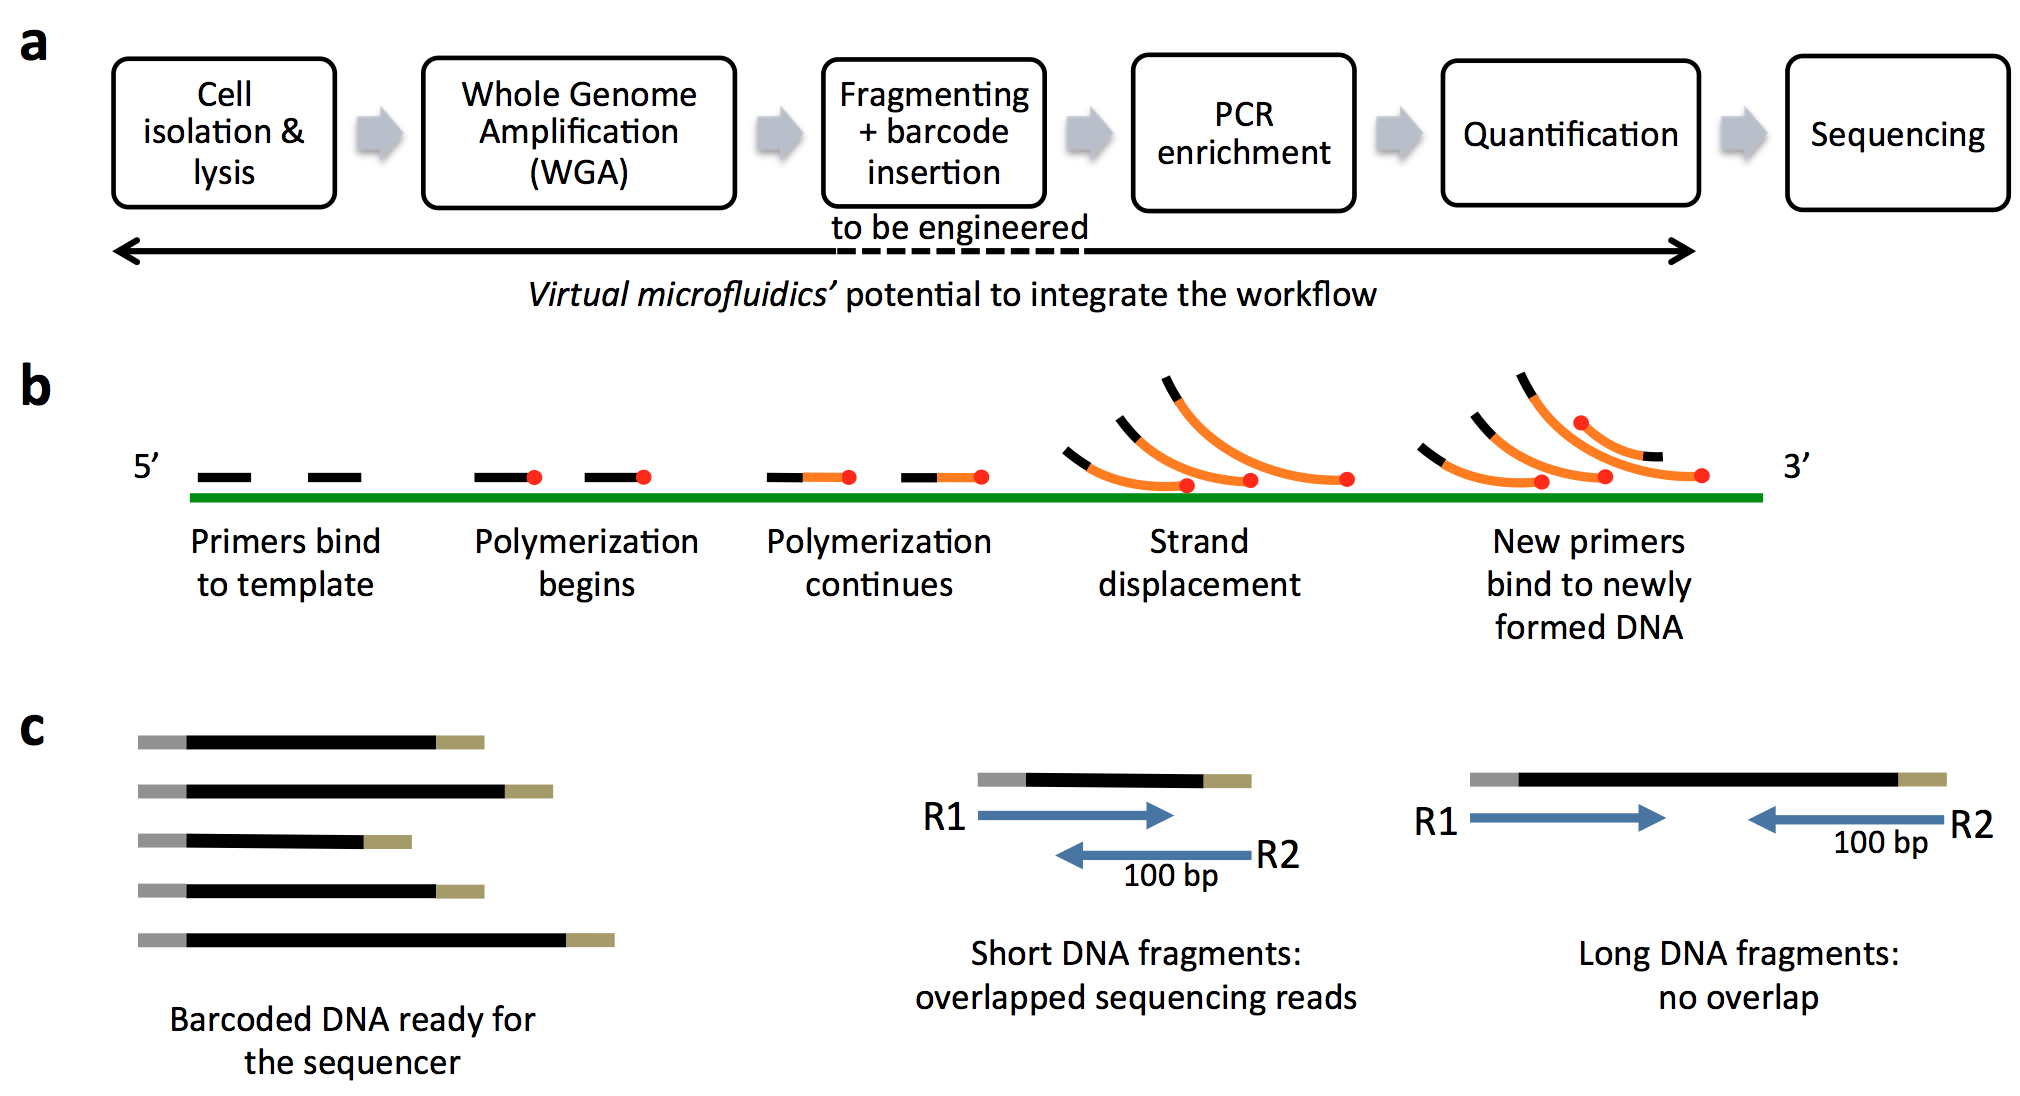
\includegraphics[keepaspectratio,width=\textwidth]{./figures/Introduction_Sequencing}
\caption[An overview of single-cell whole genome sequencing]{An overview of single-cell whole genome sequencing. (a) The single-cell analysis workflow. (b) Multiple displacement amplification (MDA) mechanism. (c) DNA are fragmented, barcoded and sequenced with pair-end sequencing.}
\label{fig:Intro}
\end{figure}

\subsubsection{Cell isolation and lysis} 
Like with single-molecule analysis, the first critical step in single-cell analysis is cell isolation. In order to separate cells of interest, relatively high-throughput technologies were adapted and developed, such as fluorescent-activated cell sorting (FACS) into multi-well plates \cite{Zhang:2006hq}, high-density microfluidic arrays \cite{Love:2013hf}, engineered lab-on-chip systems \cite{Thorsen:2002dn,Landry:2013dh,deBourcy:2014ji, Marcy:2007ip}, and multi-phase micro-droplet systems \cite{Fu:2015gl,Thorsen:2001td,Morinishi:2015jx,Mazutis:2013wn,Hindson:2013hb} (see Table \ref{tab:singlecellisolation}). %In addition to looking at the cells directly with FISH (fluorescent in situ hybridization) \cite{Kwon:2013wq,Raj:2009ds} and microarrays \cite{Neumann:2010il}. 

\begin{table}[ht!]
\caption{A comparison of single-cell isolation technologies}
\label{tab:singlecellisolation}
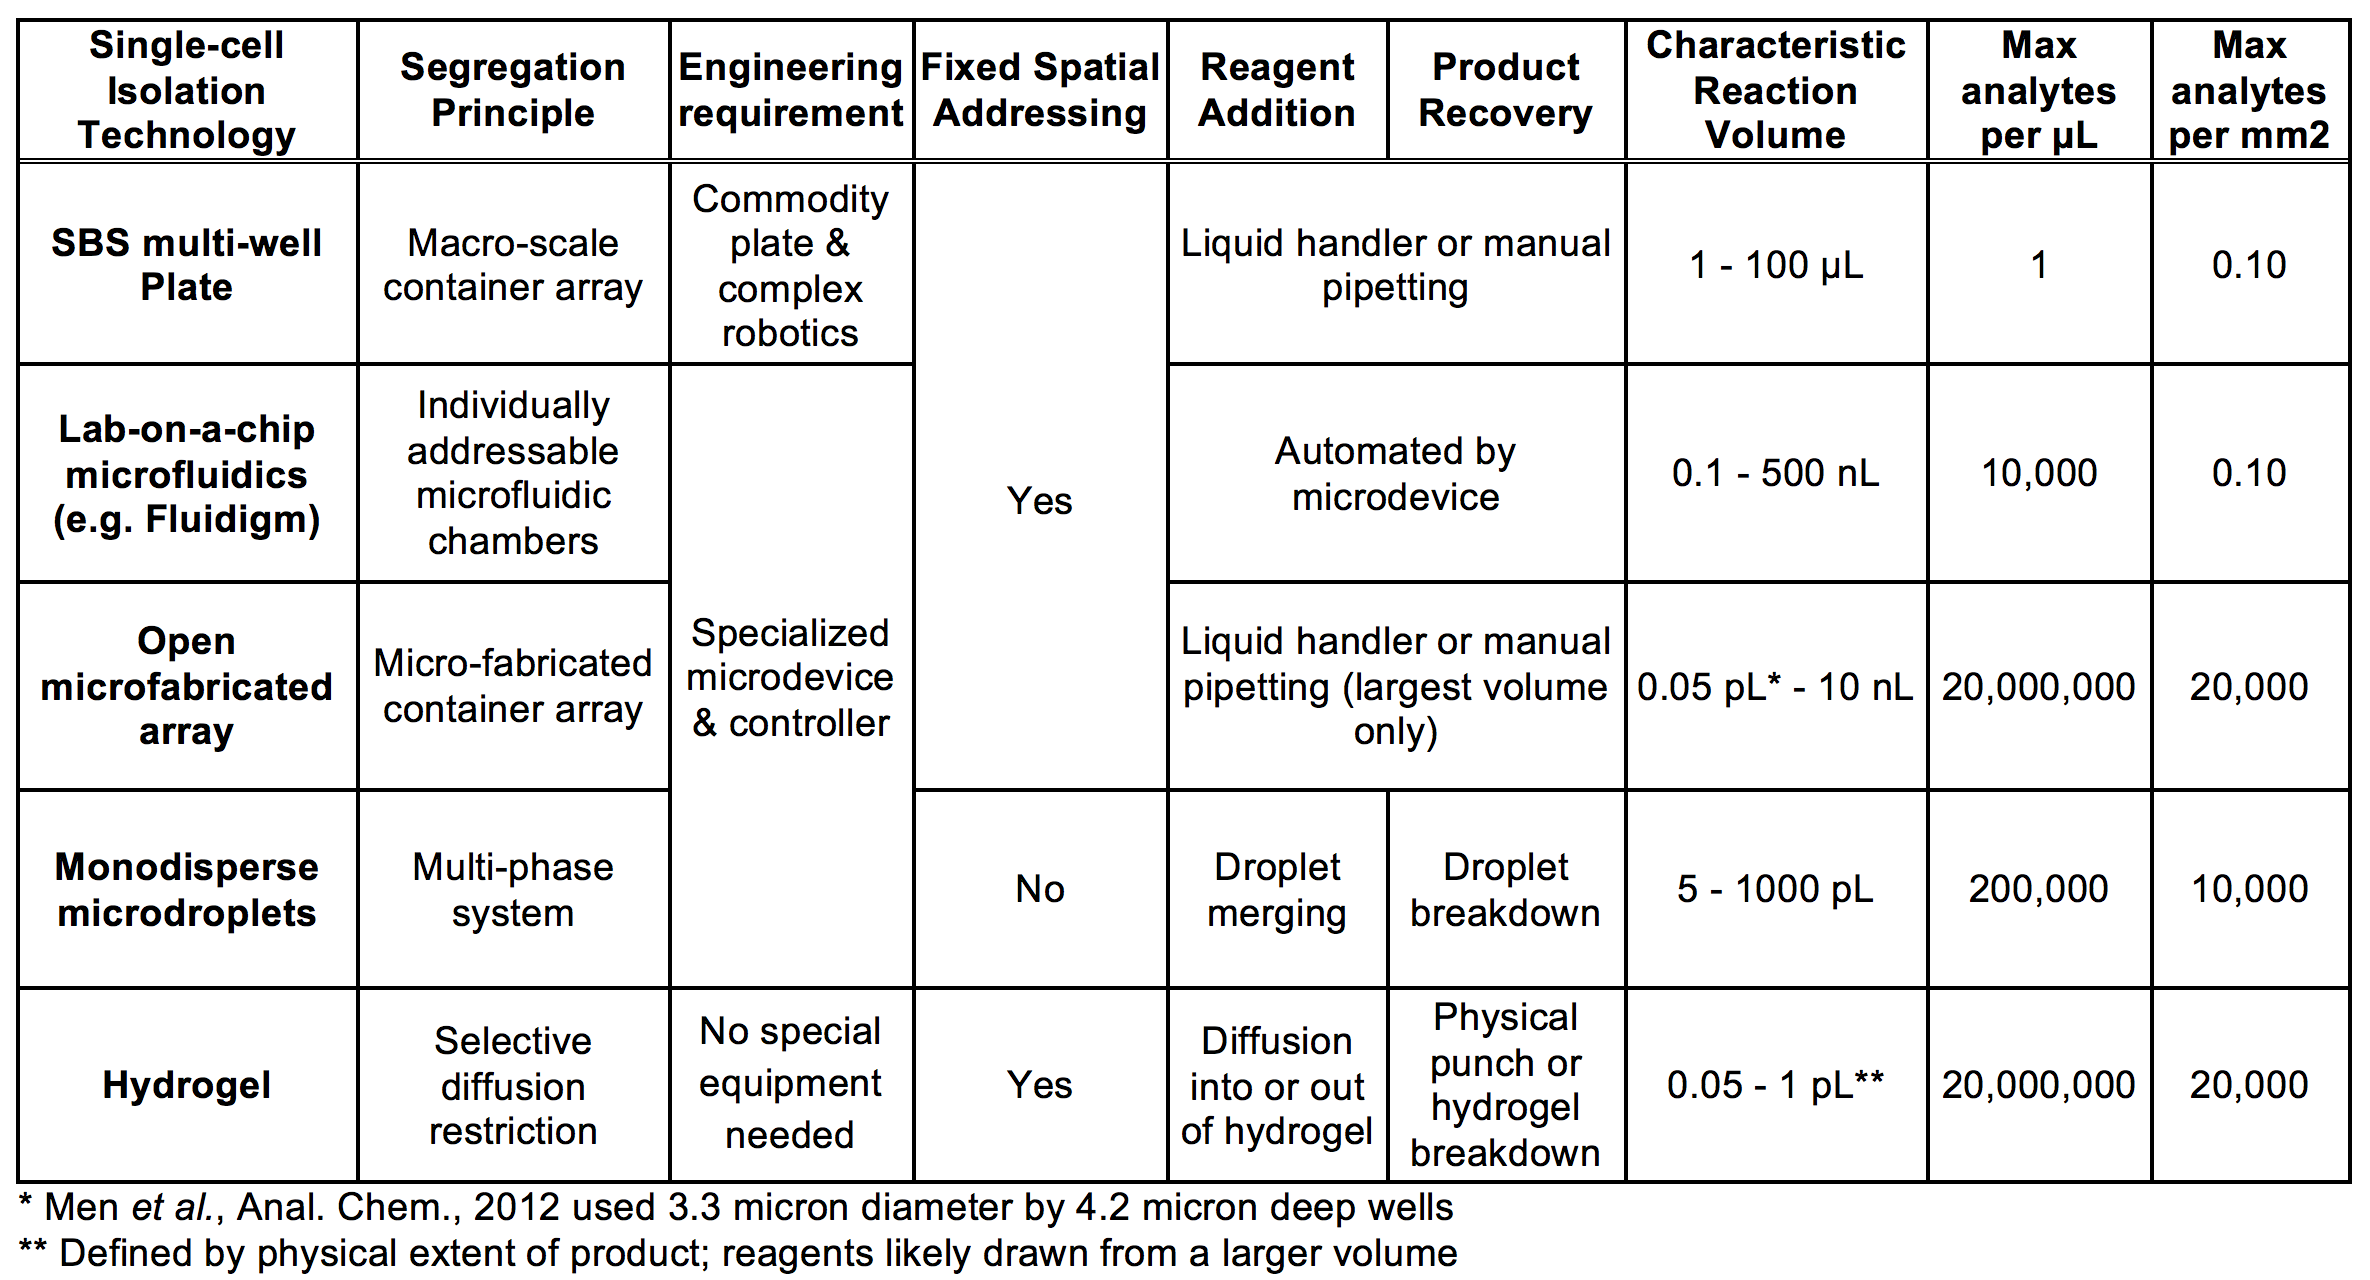
\includegraphics[width=\linewidth]{./figures/TechnologyComparisons.png}
\end{table}

Currently, the most commonly used method for cell isolation is FACS. FACS automates the process of single-cell isolation of identifiable subpopulations. The cells being sorted need to have differentiating light-scattering characteristics, express certain fluorescent markers, or to be stained by fluorescent antibodies or DNA binding dyes. Studies have used FACS with DNA binding dyes to detect and localize genetic abnormalities such as whole chromosomal deletions and aneuploidy on single cells \cite{Trask:2002iy}. The human cell size (10$\mu$m $\sim$ 20$\mu$m in diameter) and surface markers make it a suitable sample for FACS. However, it is difficult to achieve a similar success rate when separating environmental microorganisms ($\sim$ 1$\mu$m). Environmental microbial samples have a range of morphological shapes and this may result in a biased selection by light scattering, which contributes to a possible uneven representation of taxa obtained through single-cell analysis using FACS compared to bulk metagenomic sequencing. Sample preparations involving FACS, plate/well transfer, and dilution greatly increase the possibility of exogenous DNA contaminations from the lab environment \cite{Woyke:2011eg}. In the case of single-cell whole genome amplification, one single molecule of exogenous DNA can be amplified with the random priming mechanism, pose challenges in data analysis and affect the quality of \textit{de novo} assemblies \cite{Blainey:2011dt}.

To remedy the effect of sample handling, a wide variety of approaches have been explored for the microfluidic compartmentalization of single cells across a large number of small discrete reactors \cite{deBourcy:2014ji,Marcy:2007ip}. However, similar to the current methods for single-molecule analysis, existing methods require complex instrumentation and are labor intensive if set up in-house. In addition to the characteristics desired as in single-molecule assays, single-cell studies often require the compartment access for the addition and product removal of reagents and samples. A recent development of a microfluidic system that incorporates DNA purifying capability for processing microbial isolates may solve the reagent addition and retrieval problem but it is not easily accessible and scalable to single-cell resolution \cite{Kim:2017gy}. The operation of open microarray/microwells requires a specialized liquid handler such as Echo\textsuperscript{$\textregistered$} (Labcyte Inc.) and CellCelector\textsuperscript{TM} (Automated Lab Solutions). Emulsion droplet systems pose challenges in reagent addition and sample retrieval after the droplet formation. This approach is positioned well to produce a large number of picoliter partitions easily for digital counting in a single-molecule analysis that doesn't require follow up Sanger or whole genome sequencing (WGS). A recent development utilizing droplets as partitions for a single human genome WGA still requires FACS sorting or mouth pipetting for cell isolation \cite{Fu:2015gl}. 

The challenges in the single-microbe analysis are distinct from its mammalian counterpart. The difficulty in culturing prevents us from obtaining single colonies on an agar plate that provide enough starting material for sequencing (nanograms of DNA for Illumina benchtop procedures). Here is where single microbe Whole Genome Amplification (WGA) comes into play. WGA can amplify the femtograms of genomic DNA from a single microbe to nanograms (See next section on WGA for more detail). However, single microbial WGA faces numerous challenges, including low isolation efficiency and a high chance of contamination. In addition, microbial communities consist of organisms with diverse physiologies, meaning that a universal lysis strategy that works for all types is difficult due to the diverse chemical compositions of cell walls. Most lysis methods are developed for bulk samples, which may not be suitable at the single-cell level if the lysis efficiency is low \cite{Blainey:2013dp}. The undesired consequences of incomplete lysis might result in DNA locus damage and undetected microbial species. 

Alkaline lysis is the most common method for single microbe lysis today and it was first described for single cells by Raghunathan \textit{et al.} \cite{Raghunathan:2005fg}. Other supplementary methods include heat lysis, repeated freeze-thaw \cite{Swan:2011hb,Fleming:2011dv}. But the lysis success rates (obtaining pure single amplified genomes after WGA) vary widely and are often below 40\%  \cite{Stepanauskas:2012ja}. One particular type of microbes that does not lyse well in alkaline is environmental extremes, such as \textit{M. ruber} that was found in hot springs with alkaline pH \cite{NOBRE:1996ke}. On the other hand, Fleming \textit{et al.} discussed that the best strategy might be using a cocktail of enzymes that provide efficient but gentle lysis on the entire microbe types present \cite{Fleming:2011dv}. But enzymatic cocktail unavoidably contains small fragments of DNA lodged in the enzymes themselves, which become contaminants through the WGA step. The enzymatic cocktail for one single cell in isolation is often excessive as not every enzyme present will be effective in lysing and the enzyme collections might not be compatible with downstream WGA method. And it is difficult to purify such a low quantity of unamplified genomic DNA. Consequently, an effective, adaptable and clean method to enable high-throughput single-microbe isolation and lysis is needed. % Linda says fix grammer 

Cell isolation and lysis for mammalian cells is less technically challenging due to their relatively large cell size and the absence of the cell wall. The lipid bilayer cell membrane can be easily dissolved in a dilute solution of detergent, such as Triton-100X and NP-40. The enzymatic digestion and DNA deproteination methods have been widely implemented and optimized \cite{Zong:2012bs,Fu:2015gl,Leung:2016vx,Chen:2017hq,Dean:2002us}. However, it was recently discovered that many single-cell studies could be confounded by the poor data quality caused by the DNA damage after cell lysis when biological \say{variations} are in fact extensive technical biases and errors \cite{Chen:2017hq,Chen:2017dq}. For sensitive applications such as measuring the single-nucleotide variations (SNVs) in cancer cells, treating the genomic DNA with uracil-DNA glycosylase to eliminate cytosine-deaminated uracil bases can reduce a significant amount of false-positive C-to-T SNVs \cite{Chen:2017hq,Rohland:2015uk}. 

\subsubsection{Whole Genome Amplification (WGA)}
One of the most critical steps to analyze genomes of single cells is the whole genome amplification. Currently, the prevalent short-read library preparation and sequencing technologies require nanograms ($10^{-9}$ g) of input DNA for on bench procedures, while the genome of a single cell ranges from femtograms ($1.7 \times 10^{-15}$ g, \textit{Prochlorococcus} MED4) to picograms ($6 \times 10^{-12}$ g, human diploid). Thus, WGA is needed to replicate the genomic DNA from a single-cell to approximately $10^3 \sim 10^6$ fold. During the WGA process, artifacts and technical errors such as low physical genome coverage, non-uniform coverage due to GC\% bias, false-positive (FP) errors and false-negative errors are often introduced. Achieving a high physical coverage of the genome with a low error rate is crucial for calling mutations accurately at the same regions of multiple single cells. There is a need for WGA method improvement that provide high-quality single-cell WGA data in above-mentioned criteria.

Multiple Displacement Amplification (MDA) \cite{Dean:2002us} is a well-characterized WGA method commonly used to enable single-cell genome sequencing \cite{Marcy:2007il,Fu:2015gl,Zhang:2006hq,Raghunathan:2005fg,Pamp:2012cj,Dodsworth:2013ih,Hess:2011gu}. MDA uses $\Phi$29 polymerase with a strong strand displacement property and random exonuclease-resistant 6 bp primers to produce longer than 12 kbp amplification products at $30^{\circ}$C (Fig. \ref{fig:Intro}b). MDA provides greater genome coverage than the PCR-based methods such as degenerate oligonucleotide primed PCR (DOP-PCR) and lower error rate than \textit{Taq} and \textit{Bst} polymerases owing to the high fidelity of $\Phi$29 polymerase \cite{Dean:2002us}. However, the exponentially amplified genome through MDA has regions that are overrepresented and this bias positively correlates with the fold of amplification \cite{deBourcy:2014ji}. In addition, the random priming nature allows DNA amplification on any exogenous DNA contaminants, posing a threat in raising the false-positive rate in new genome discovery. 

Recent technology innovations have been focused on improving MDA performance by varying methods of physical partitions. It has been shown that contaminating DNA was largely eliminated by moving MDA from microliter reaction volumes in tubes to a microfluidic format that used nanoliter volumes \cite{deBourcy:2014ji}. The MDA amplification gain is also limited by the nanoliter volume, thus improving its coverage uniformity. The trend of using sub-microliter partitions lead to the development of emulsion WGA (eWGA) \cite{Fu:2015gl} and Nanodrop MDA \cite{Leung:2016vx}. In eWGA, a single cell is FACS sorted and lysed, then randomly distributes in a large number ($10^5$) of picoliter droplets. Each droplet contains zero to a few fragments of DNA that go through MDA reaction. The results showed improved uniformity and high coverage at the amplification gain of 2 \times $10^6$ for human cells. This improvement is made possible by isolating different parts of the genome during MDA. Thus, this way, the over-amplified fragments would not compete globally with fragments in different droplets that have a late start in MDA. This results in a more uniform amplification depth that improves copy number variations calling accuracy. Nanodrop MDA utilizes commercially available piezoelectric non-contact liquid dispenser to deposit nanoliter-ranged drops sequentially onto a planar substrate and each drop's single-cell occupancy depends on Poisson loading. MDA reagents are added to drops containing single cells in the same way and each 100 nL reaction is covered with mineral oil to prevent evaporation. Both eWGA and Nanodrop methods have shown improvements in terms of data quality in genome coverage percentage and coverage uniformity. But both methods still rely on FACS sorting or liquid dispensing and the rate of artifacts formed in MDA was not characterized. High level of chimeric DNA rearrangements (artifacts) can lead to inaccurate genome structural variation analysis but are rarely analyzed in single-cell technology development. We will discuss in depth on this subject in Chapter 4 and how it can impact microbial \textit{de novo} assembly, investigating mutational mosaicism in neurons, and single-cell cancer research. 

%Quantifying the mutation rate and the mutation heterogeneity in cancer are difficult tasks to tackle. These genomic changes are summarized into 3 main categories: single nucleotide variations (SNVs), Copy Number Variations (CNVs), and structural variations. Among those, genome Structural Variations (SV)(including inversion, translocation, duplication) are an important source of cancer cell heterogeneity and brain developmental diseases but remain technical challenging to detect from bulk sequencing \cite{Norris:2016ec}. There is an unmet need for clinical assays that can cheaply and rapidly profile SVs in solid tumors in a low-input or single-cell resolution \cite{Macintyre:2016hw}. The mutation definition in this context includes a wide range of heritable changes in the nucleotide sequence of DNA, such as single nucleotide point mutation, gene insertion, deletion, rearrangements and large-scale chromosomal abnormalities (trisomy, inversion, translocation, etc). 

In addition to improving the experimental setup for MDA, efforts have been made to develop new WGA chemistry that linearly amplifies the genome to reduce biased coverages the dependence on complex instruments \cite{Zong:2012bs,Chen:2017hq}. The most recent method LIANTI (Linear Amplification via Transposon Insertion) utilizes direct transposon insertion and \textit{in vitro} transcription to linearly amplify RNA copies of the genome. This method eliminates the random non-specific priming used in traditional MDA method and has shown to improve coverage uniformity and reduce the false-positive rate in calling single nucleotide variations. The lower error rate is due to linear amplification's random error position on the same template. By sequencing single cells to a high depth (30$\times$), amplification error would be corrected, which leads to fewer false positive calls. LIANTI has a huge potential for its wide adoption as the next generation of WGA method. According to the analysis in chapter 4, a majority (70\%) of LIANTI's sequencing reads contain barcode information and poor quality reads. A large portion of sequencing effort is wasted as a result (\$2500 $\times$ 70\% = \$1750 wasted per cell in sequencing cost). More work needs to be done to integrate the transposon barcode insertion and its downstream library preparation.

After WGA, purified DNA will go through library preparation - fragmentation and barcode insertion. Accurately purified and quantified libraries, in terms of both size ranges and quantities, will be loaded onto the sequencer (Fig. \ref{fig:Intro}d). 
 
Overall, the single-cell sequencing process from having cells in suspension to obtaining sequencing data is highly fragmented in terms of technology implementation. eWGA and LIANTI have to rely on traditional FACS sorting or mouth pipetting while Nanodrop requires sequential depositions for both cell isolation and reagents addition. Efforts have been made to integrate library preparation in microfluidic chips \cite{Kim:2017gy} and to package cell isolation and WGA in a commercially available droplet system (10X Genomics). Both examples are either cumbersome to implement or expensive to purchase. For 10X Genomics, for instances, it costs \$ 50K per machine. Researchers working in microbial discovery and oncology studies are looking for ways to conduct single-cell sequencing with an economically reasonable and technically manageable method for a large number of single cells. Independent innovations addressing different stages of single-cell sequencing will push the field forward in small steps. Ideally, an integrated approach that provides an accessible platform to streamline the process while produces high-quality data is needed to realize single-cell sequencing's huge potential in scientific discovery and biomedical field. 

\section{\textbf{\textit{Virtual Microfluidics}} for
digital quantification and single-cell sequencing}
In the introduction, we reviewed the increasing scientific and biomedical need for single-molecule and single-cell analysis and their current technology landscape. Much improvement is needed to bridge the gap between the current technology state and the wide adoption of the method. The necessary improvement areas I have discussed include high-throughput, the data quality, the ease of implementation, optical enrichment properties and the process integration. Thus, I developed the method \textit{virtual microfluidics} to make an improvement in above-mentioned areas and to help push the single-molecule and single-cell analysis fields forward (Fig. \ref{fig:VM1}). 

\begin{figure}[ht!]
\centering
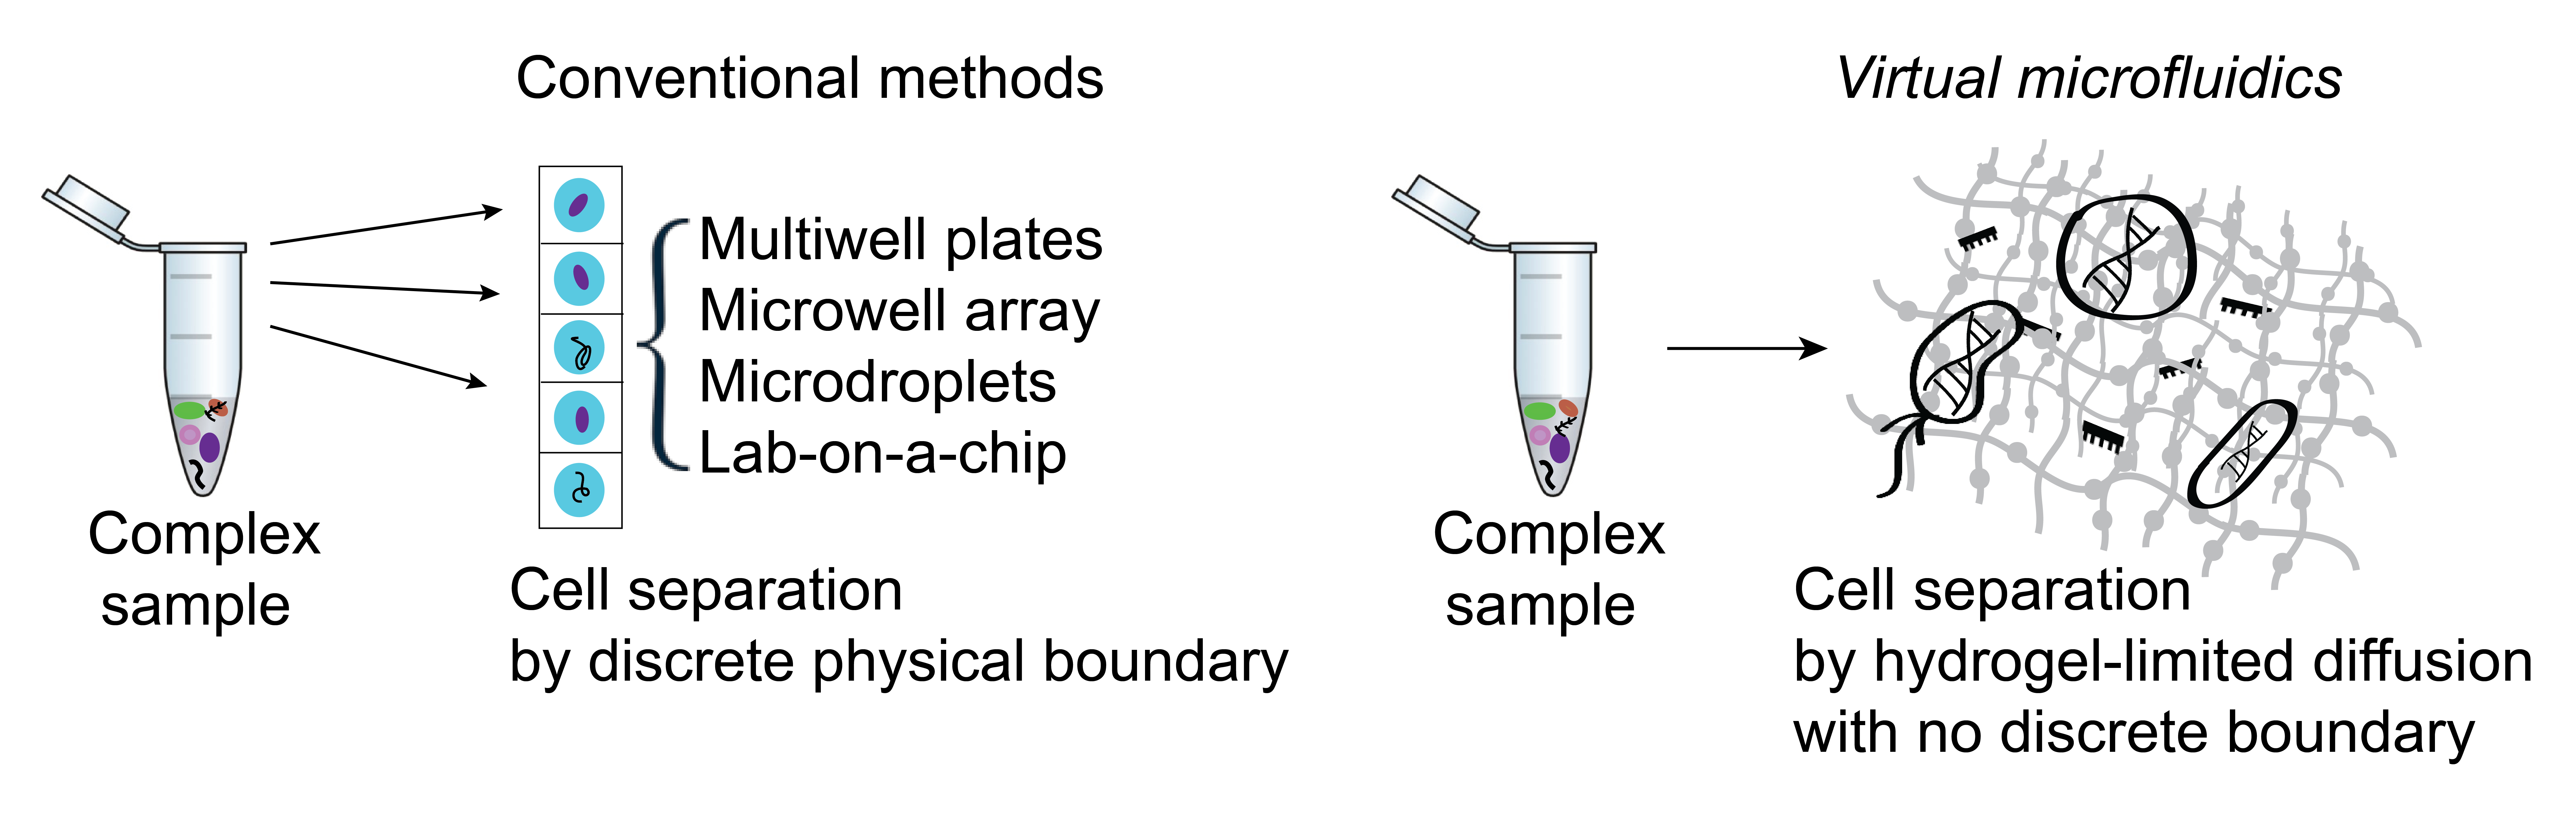
\includegraphics[keepaspectratio,width=1\textwidth]{./figures/Thesis-20.png}
\caption[Conventional methods vs. \textit{virtual microfluidics}]{Conventional methods vs. \textit{virtual microfluidics}. Conventional single-cell analysis methods
require discrete physical boundaries. \textit{Virtual microfluidics} relies on hydrogel-limited diffusion to compartmentalize templates and reaction products.}
\label{fig:VM1}
\end{figure}

Single-molecule and single-cell studies require individual molecules or cells separated in partitions. But instead of creating physical partitions to isolate cells, we decided to build \say{invisible} dividers around them. Passive segregation of single molecules and the product of genome amplification would be able to facilitate the genomic analysis of thousands of nucleic acids in parallel. In order to achieve this, a porous structure that is able to fix many molecules and provide an aqueous environment for DNA amplification was chosen. Thus, the \textit{virtual microfluidics} system was created to enable single-cell WGA \textit{en masse} in poly(ethylene glycol) (PEG) hydrogel. The hydrogel properties allow reagent exchange by diffusion, imaging accessibility, product retrieval easiness and improved WGA performances using MDA compared to instrumentation-based methods. \textit{Virtual microfluidics} is also a versatile and compatible platform to integrate PCR, MDA and in-gel library preparation methods, which holds great promise in integrating single-cell analysis field and pushing the wider adoption of the technology (Fig. \ref{fig:FigAbstract}) . 

\begin{figure}[ht!]
\centering
\includegraphics[keepaspectratio,width=1\textwidth]{./figures/SolidPhaseWGAvsTraditional}
\caption[A graphical abstract of the \textit{virtual microfluidics} technique]{A graphical abstract of the \textit{virtual microfluidics} technique.}
\label{fig:FigAbstract}
\end{figure}

In chapter 2, I will characterize \textit{virtual microfluidics} in quantifying DNA targets for single-molecule analysis and demonstrated its improvement in the ease of implementation and its wide dynamic range in quantifying DNA targets. In chapter 3, \textit{virtual microfluidics} is applied to mixed cultures of bacteria and the human gut microbiome. It produces single amplified genomes with excellent coverage uniformity and markedly reduced chimerism compared with liquid MDA reactions. We demonstrate single-cell sequencing on human gut microbiome samples and obtain 117 pure single draft genomes that enabled the identification of more than 10,000 horizontally transferred genes that have unique population-specific and individual-specific features \cite{Brito:2016cd}. In chapter 4, I will show how \textit{virtual microfluidics} reduces the amount of chimera artifacts from MDA on single amplified human genomes compared to above-mentioned technologies. 
 
The results described in chapter 2 and 3 have been published as Xu \textit{et al.} Nature Methods. 2016.

The single-cell dataset generated from the human gut microbiome contributed to the publication of Brito \textit{et al.} Nature. 2016.


\chapter{\textbf{\textit{Virtual Microfluidics}}: a hydrogel-based system for simple and robust DNA digital quantification using \textit{in situ} amplification}
This thesis chapter is reproduced from a previously published paper, Xu \textit{et al.}, Nature Methods, 2016.\cite{Xu:2016wt}. Experiments and data analysis were performed by Liyi Xu. 

% \section{Abstract}
% We have developed the hydrogel-based \textit{virtual microfluidics} as a simple and robust alternative to complex engineered microfluidic systems for the compartmentalization of nucleic acid amplification reactions. We applied in-gel digital PCR (dPCR) and in-gel digital multiple displacement amplification (dMDA) to purified DNA templates in the system and demonstrated accurate digital counting of nucleic acid targets. We characterized the dynamic range of the digital amplification and investigated factors controlling the amplification cluster size. We expect \textit{virtual microfluidics} to find application as a low-cost digital assay platform that is highly accessible with an extensive dynamic range. 
%\textit{virtual microfluidics} has the potential to be used as an accessible, versatile low-input DNA analysis tool for various research and clinical applications. 

\section{Introduction}

The absolute quantification of DNA sequences and fragments in genomics \cite{Blainey:2011dt} and prenatal diagnostics \cite{Lo:2007hb} requires assays that enable parallel clonal nucleic acid amplification. DNA quantification by amplification also is needed to overcome nonspecific background for the detection of rare sequence targets in microbial communities and blood-plasma-based diagnostics \cite{Huggett:2015hp,Gevensleben:2013kg,Kuypers:2017it,Johnson:2002wb}.

% Assays involving highly parallel clonal nucleic acid amplification are needed for accurate copy-number analysis with absolute quantification of DNA sequences\cite{Sykes:1992tm,Vogelstain:1999ve} and fragments\cite{Blainey:2011dt} in genomics and prenatal diagnostics\cite{Lo:2007hb}. Such assays are also needed to overcome nonspecific background for the detection of rare sequence targets in microbial communities and blood-plasma-based diagnostics \cite{Huggett:2015hp,Kuypers:2017it,Johnson:2002wb,Gevensleben:2013kg}. 

The traditional method of single-molecule studies requires individual molecules separated in partitions. It is commonly done in engineered microfluidic systems and multi-phase micro-droplet systems, which prevent a broader deployment of digital assays in research labs and in the clinic. Instead of creating physical partitions to isolate individual contents, we decided to build \say{invisible} dividers around them. Passive segregation of single molecules and the product of genome amplification will be able to facilitate genomic analysis of thousands of nucleic acids in parallel. In order to achieve this, a porous structure that is able to fix many molecules and provide a liquid environment for DNA amplification is needed. 

Inspired by earlier work on culturing microbes in hydrogels \cite{Podar:2009ks}, polymerase cloning in polyacrylamide gels using PCR \cite{Mitra:1999ty} and in agarose gels using MDA in conjunction with flow cytometry \cite{Allen:2011jn}, we developed and tested bulk poly(ethylene glycol) (PEG) hydrogels as a general and facile platform for compartmentalizing single molecules and single cells without discrete partitions. This approach, which we call `virtual microfluidics' (Fig. \ref{fig:VM1} and \ref{fig:GelStructure}), enables massively parallel single-molecule amplification in virtual sub-divisions without the need for engineered micro-devices, multi-phase liquid systems, or instrumentation for cell sorting or microfluidics control. We selected hydrolytically degradable PEG hydrogels that covalently crosslink under mild conditions \cite{Raeber:2005cq}. The chemically selective crosslinking reaction used in our method does not damage templates or inhibit subsequent reactions and forms gels that are stable to high temperatures. The mesh size of the PEG gel allows diffusion of small molecules, oligonucleotides, and enzymes but immobilizes cells and high-molecular-weight nucleic acids \cite{Wu:2009ez}. If desired, PEG gels can be functionalized to selectively immobilize low molecular weight species by attachment to the gel matrix \cite{Phelps:2011dka}.

\begin{figure} 
\centering
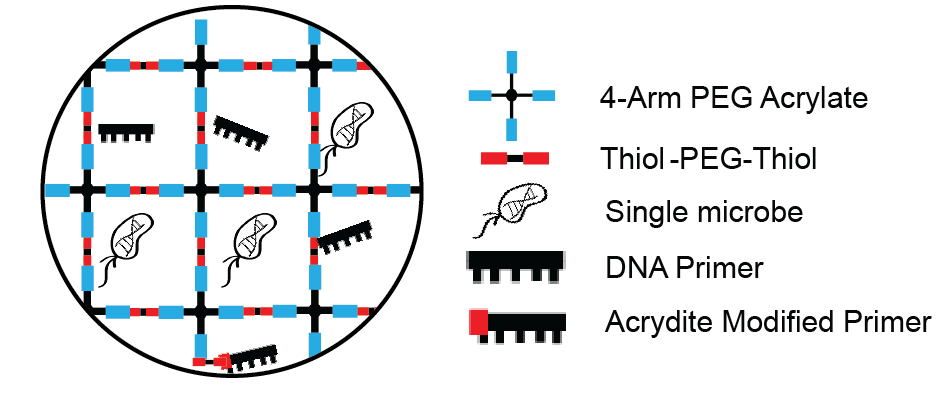
\includegraphics[keepaspectratio,width=0.6\textwidth]{./figures/SolidPhaseWGA-21}
\caption[The \textit{virtual microfluidics} hydrogel structure.]{The \textit{virtual microfluidics} hydrogel structure.}
\label{fig:GelStructure}
\end{figure}

Hydrogels are formed by crosslinking polymer chains through physical, ionic or covalent interactions and are best known for their ability to absorb water \cite{Elisseeff:2008cm}, which makes them a perfect candidate for solid-phase DNA amplification (solid-phase here means in-gel, compared to liquid-phase reactions). Previously, the polyacrylamide hydrogel has been used as a scaffold for solid-phase DNA amplification \cite{Mitra:1999ty}. However, polyacrylamide gel crosslinks with the free radicals initially produced by ammonium persulfate or by photochemical polymerization. The free radicals have been found to inhibit reverse-transcription PCR and inhibit DNA dyes such as SYBR Green and LC Green plus \cite{Atrazhev:2010ex} for real-time monitoring, while photochemical polymerization might introduce DNA damage to the target of interest. Such DNA oxidative stress caused by the addition of free radicals is a pervasive cause of sequencing error and directly confound variant identification \cite{Chen:2017dq}. Luckily, a new generation of PEG-based multi-arm hydrogel has been developed that provide many advantages for our purpose \cite{Tan:2010by}. Specifically, 4-arm PEG hydrogel with various end moieties has been applied for gene delivery and building 3D scaffolds for tissue engineering. The hydrogels are formed via Michael addition chemistry by reacting a 4-arm acrylate terminated PEG with a thiol-functionalized PEG \cite{Li:2012bd}. The use of Michael addition chemistry allows for \textit{in situ} hydrogel formation under physiological conditions, which will cause minimal damage to the DNA and cells of interest in broad applications. In addition, while acrylamide powder is neurotoxic, 4-arm PEG components pose no such harm to researchers. In terms of mesh size, Raeber \textit{et al.} and Kraehenbuehl \textit{et al.} have shown that 4-arm PEG's pore size is between 25nm and 100nm depending on the weight percentage \cite{Raeber:2005cq,Kraehenbuehl:2008do}

% , which has a potential to be applied for optimizing the DNA amplification cluster size for subcellular localization application. 

PCR and MDA amplification, application and tech similarities and differences 


\section{Results and Discussion}
\subsection{Digital PCR in-gel characterization}

\begin{figure} 
\centering
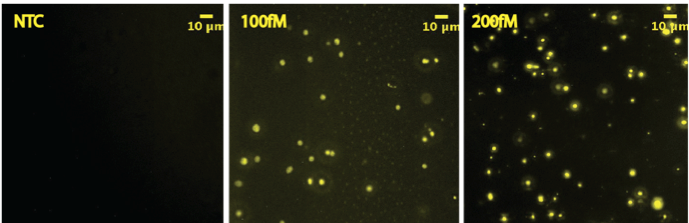
\includegraphics[keepaspectratio,width=1\textwidth]{./figures/dPCR_Capillary.png}
\caption[DNA amplification clusters from PCR in hydrogel in a capillary tube.]{DNA amplification clusters from PCR in hydrogel in a capillary tube. Images are taking using a Nikon wide-field fluorescent microscope. The concentration of DNA template was labeled in units of femtomolar(fM). The capillary tube is 50 $\mu$m tall.}
\label{fig:dPCR_Cap}
\end{figure}

In order to characterize the technology, purified lambda phage DNA is used as the template to conduct DNA amplification in the PEG hydrogel. \textlambda DNA is a common, well-characterized substrate for restriction endonucleases and its sequence and properties have been well-understood \cite{Fu:2011wc, Robertson:2006gi}. The 48502 bp length acts as a useful proxy for genomic DNA from bacteria or mammalian cells. In order to quantify the robustness of solid phase DNA amplification and estimate the dynamic range of the technology, a range of DNA template concentrations from serial dilutions of a stock were used. Reaction components consisting of 4-arm PEG-acrylate, dithiol-PEG, PCR reaction buffer, primers, dNTP, DNA polymerase and template are mixed thoroughly before loaded in a reaction chamber. Various experimental configurations such as PDMS channels, capillary glass tubes (Fig. \ref{fig:dPCR_Cap}), thin PDMS wells (10 $\mu$m to 50 $\mu$m), and frame-seal chambers (Biorad) have been tested, with the frame-seal chamber (Fig. \ref{fig:FigAbstract} in chapter 1 and \ref{fig:dPCR_FS} in methods) proved to be the most efficient and consistent loading method. Several types of DNA polymerase with different levels of fidelity, 3'-5' proofreading, and primer extension capacity, such as Jumpstart \textit{Taq}, Vent (exo-), Vent, have been tested in hydrogel for amplification optimization. Fig. \ref{fig:dPCR_Calibration} showed accurate digital counting was achieved by PCR in gel. 

\subsection{Digital MDA in-gel characterization}
In addition to PCR in hydrogel, Multiple Displacement Amplification (MDA) is conducted for whole genome amplification in hydrogel. MDA \cite{Dean:2002us} is a popular amplification method for single-cell genome sequencing \cite{Marcy:2007il,Fu:2015gl,Zhang:2006hq,Raghunathan:2005fg,Pamp:2012cj,Dodsworth:2013ih,Hess:2011gu}. To evaluate the \textit{virtual microfluidics} concept for WGA, we tested dMDA \cite{Morinishi:2015jx,Blainey:2011dt} of purified, diluted Lambda phage DNA in the hydrogel format (Fig. \ref{fig:dMDA}a-c, Fig. \ref{fig:dMDA_Quant} and Methods). Our estimate of 10 pg MDA product per cluster (Fig. \ref{fig:dMDA_MammalianEcoliCluster}) suggests that we approached endpoint product concentrations typical of conventional liquid MDA reactions (\ensuremath{\sim}800 ng\slash $\mu$L) \cite{Blainey:2013dp}. We varied parameters to test how \textit{in situ} single-molecule MDA reactions can be controlled (Fig. \ref{fig:dMDA} and Fig. \ref{fig:dMDA_Quant}), observing that the smaller pore sizes in higher density gels limit the spread of DNA products.

\begin{figure}
\centering
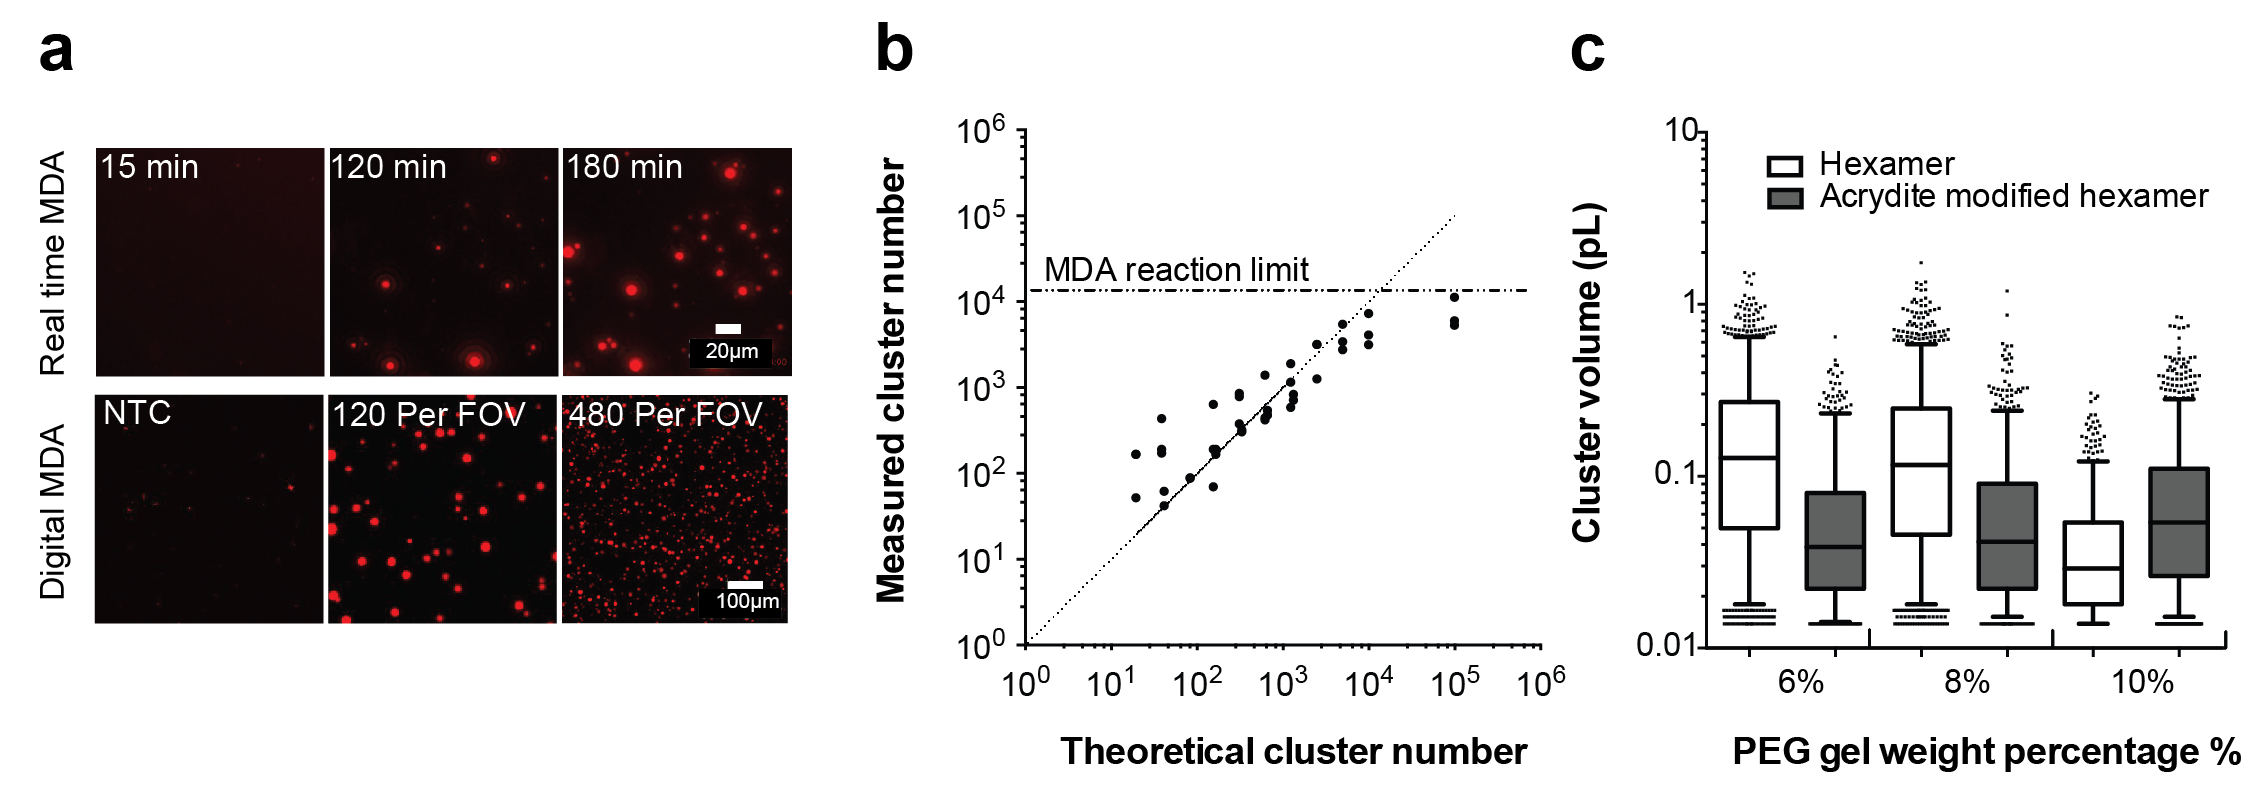
\includegraphics[keepaspectratio,width=1\textwidth]{./figures/Thesis-21.png}
\caption[Digital single-molecule MDA in hydrogel (Lambda phage DNA).]{Digital single-molecule MDA in hydrogel (Lambda phage DNA).(a) Real-time and digital MDA in PEG hydrogel. Top, time-lapse
epi-fluorescence images (SYTOX Orange DNA stain) illustrate MDA cluster growth from individual template molecules. Bottom, DNA cluster number increases with template concentration. FOV, 650 nm $\times$ 650 nm field of view. NTC, no DNA template control. (b) Calibration curve illustrates linear relationship between template concentration and cluster number (n = 2 or 3 FOV at
each concentration). (c) MDA cluster size is correlated with gel weight percentage and affected by acrydite-modified hexamer anchorage. Data are shown as 5 \textendash  95$\%$ box plots with scattered outliers and center line for median. (n = 1334, 1587, 684, 704, 869 and 1301).}
\label{fig:dMDA}
\end{figure}

Similar sample preparation and loading method are used for dMDA compared to dPCR in the hydrogel. The only difference for dMDA in the hydrogel is the UV decontamination step on all reaction components except the polymerase. The study by Woyke \textit{et al.} has shown that the calibrated UV decontamination step can effectively remove contaminant DNA without introducing significant coverage biases or variants \cite{Woyke:2011eg}. 

\begin{figure}
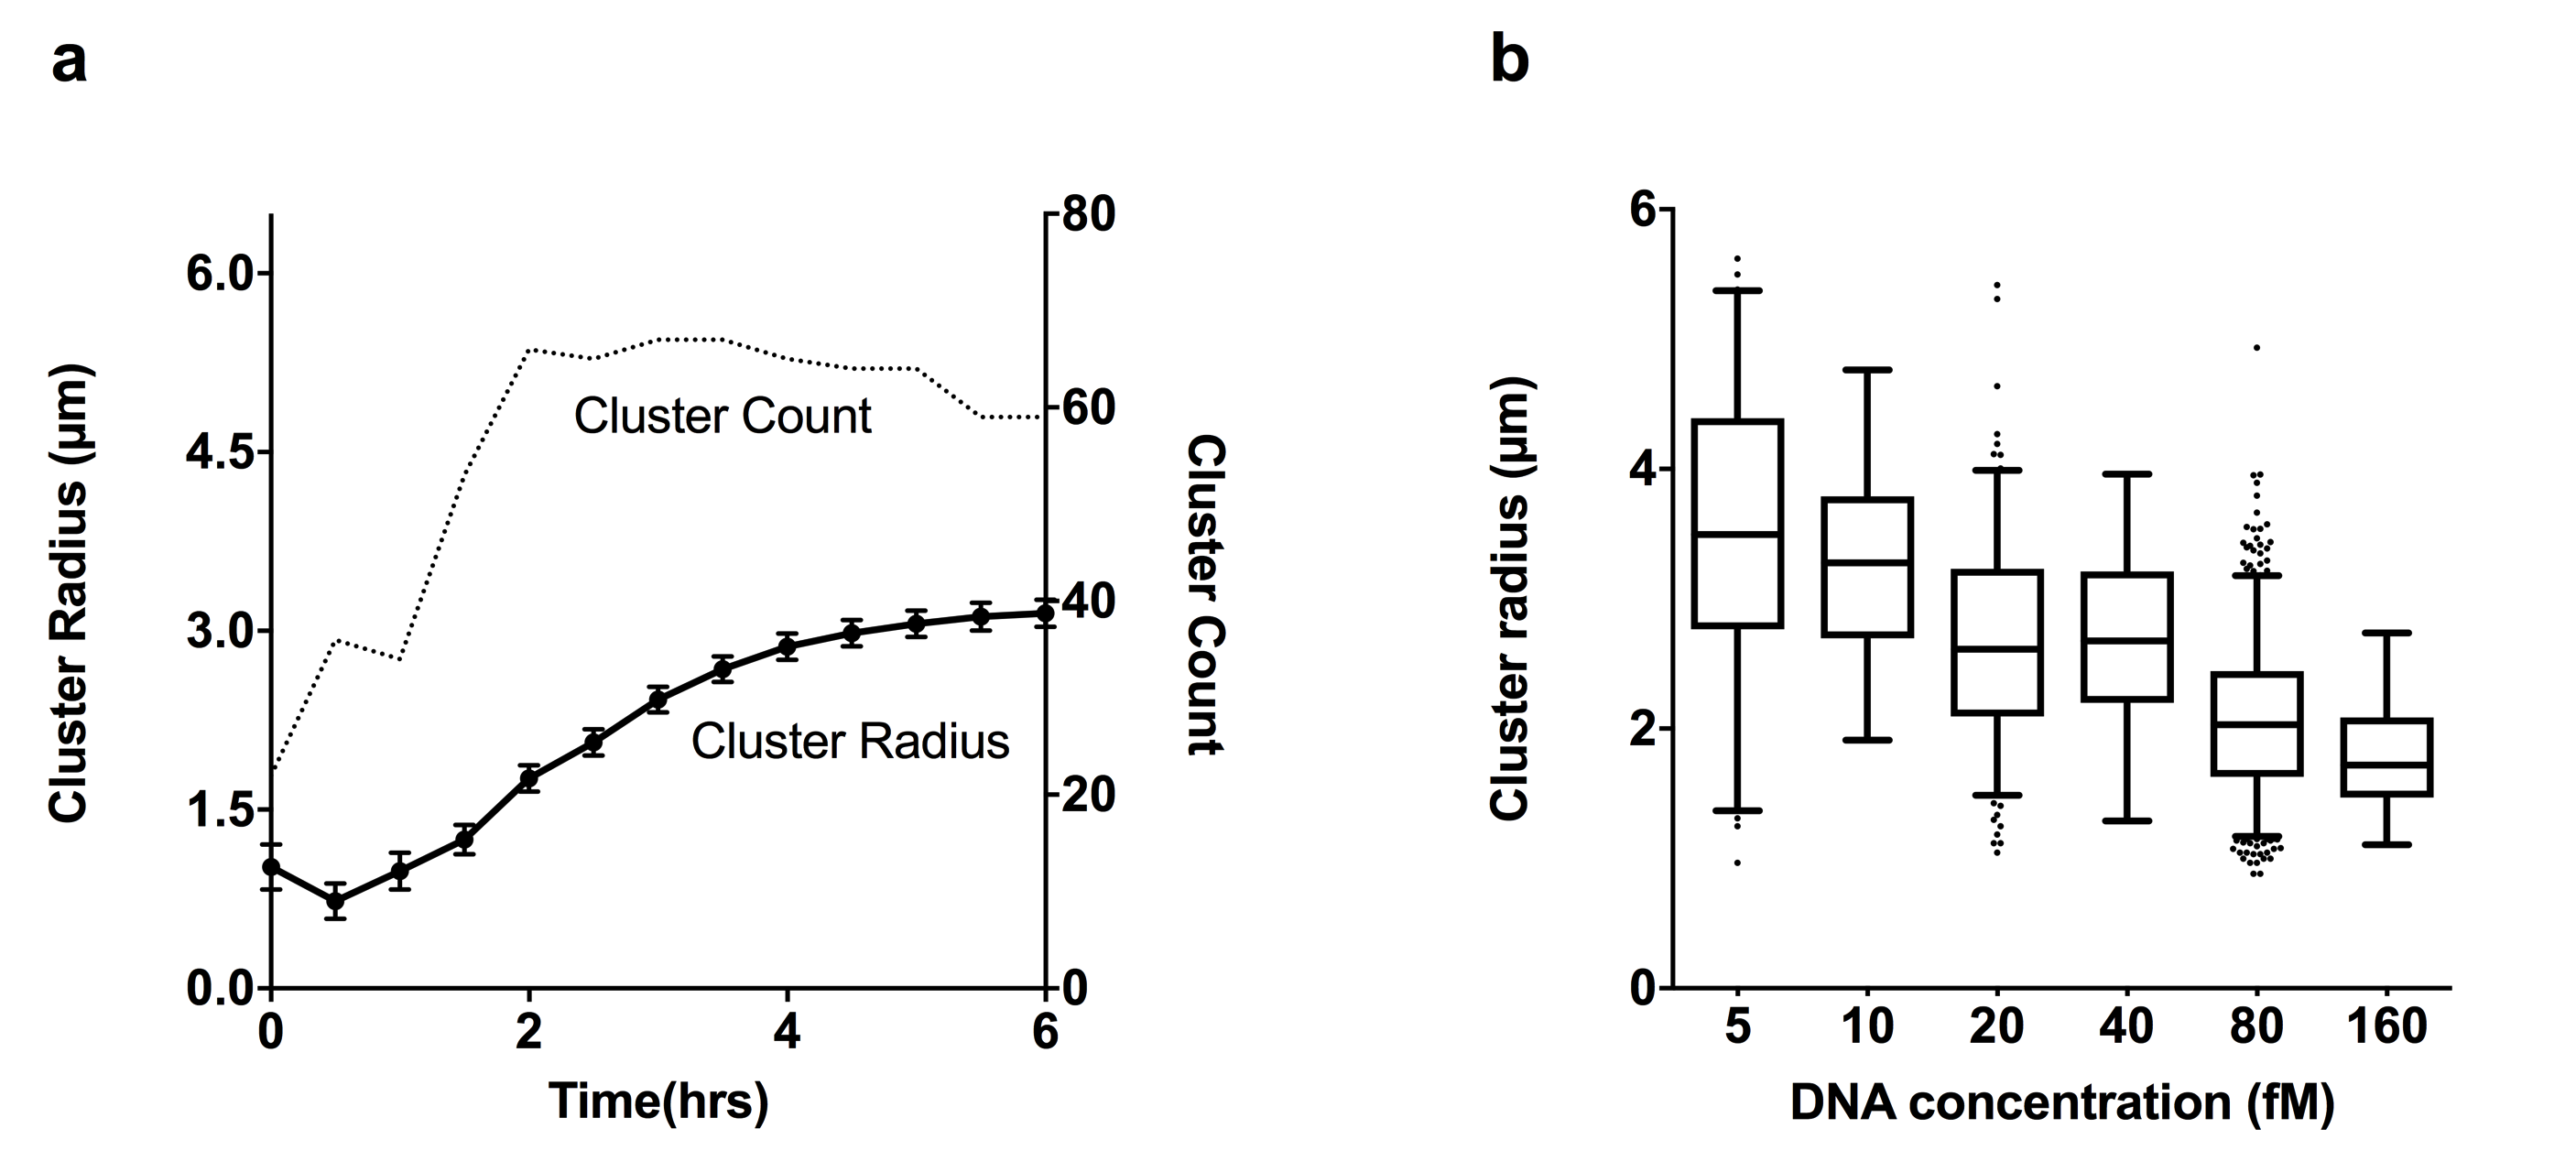
\includegraphics[keepaspectratio,width=1\textwidth]{./figures/Supp1_4.png}
\caption[Real time dMDA and MDA cluster size]{Real time dMDA and MDA cluster size. (a) Real time digital MDA for quantification of cluster growth (mean radius ± SEM) and count with time. The zero time point cluster count and radius data points reflect the properties of fluorescent contaminants. (b) MDA cluster size decreases with increasing DNA template concentration with the same gel condition. Data is shown as 5 \% - 95 \% box plot with outliers scattered and the centerline as the median. (n = 2 fields of view at each concentration, number of clusters for each field of view is: n = 43, 62, 89, 88, 191, 167, 321, 305, 478, 542, 711, 833).}
\label{fig:dMDA_Quant}
\end{figure}

With the success of dPCR and dMDA in the hydrogel, a robust but straightforward image analysis method is needed to obtain the absolute count of DNA molecules and the size of DNA amplification clusters. Currently, image analysis is conducted on the raw confocal stacks using Fiji Image J. Image J particle analyzer plug-in is widely used for counting particles and cells. Confocal stacks were taken with consistent laser power and integrated with a Z intensity gradient to minimize cluster fluorescent saturation. Each gel stack, roughly 300 $\mu$m thick, was first projected in Z direction with the maximum intensity for a faster 2D processing. Then, a thresholding algorithm is chosen manually based on the visual comparison between the original projection and the thresholded image. This image analysis method has been proved effective in measuring the number and the size of DNA amplification clusters. However, a more consistent and robust image analysis routine might be needed for a higher-sensitivity application. 

\subsection{DNA amplification cluster analysis}
Understanding the mechanism of cluster growth and effectively controlling the size of the end product are keys ensuring the broader applicability of this technology. Key parameters include initial DNA concentration, hydrogel weight percentage, primer modification chemistry and amplification time. One hypothesis regarding the size of clusters is that with a higher PEG hydrogel weight percentage, tighter clusters should be generated. Higher PEG weight percentage means more 4-arm PEG acrylate and dithiol-PEG in a fixed volume. Thus, the hydrogel network will provide a smaller mesh size for DNA template and prevent amplification product from moving further due to restricted diffusion. Another possibility is that a tighter mesh size might compromise the robustness of DNA amplification reaction due to the physical impedance. 

Another way to control the DNA amplification cluster size could be to add a chemical moiety to the primers. Acrydite modification on DNA probes has been used frequently to attach primers to various hydrogel platforms \cite{Mitra:1999ty}. In this case, acrydite reacts with the part of the thiol groups on dithiol-PEG and unreacted thiol groups will crosslink with 4-arm PEG acrylate. Varying the modified primers' concentration and its ratio to standard primer concentration gave us new insights on how to control cluster size (Fig. \ref{fig:dMDA}c). 

Meanwhile, real-time monitoring on the DNA clusters' growing helps determine the optimal reaction time and cycle numbers for both MDA and PCR reactions (Fig. \ref{fig:dMDA_Quant}a). It will be also useful to help decide on a cut-off reading time to prevent false-positive readings including the small primer-dimer clusters and clusters from short DNA fragments mixed in a genomic DNA sample (Fig. \ref{fig:dMDA_Quant}a).

\subsection{Dynamic range of in-gel digital MDA}
When the input for digital MDA is very low (fewer than 100 per field of view), molecular counts are significantly inflated by contaminating fluorescence signals (contaminating DNA fragments or particles) that are not differentiated from true counts by our image analysis algorithm. At high target concentrations, the DNA clusters crowd one another, limiting the maximum useful concentration to 10,000 DNA molecules per field of view. For MDA, the smaller cluster sizes observed at higher template concentration (Fig. \ref{fig:dMDA_Quant}b) benefit assay dynamic range by improving cluster identifiability at the highest template concentrations. Based on our estimate of 10 pg DNA per cluster (Fig. \ref{fig:dMDA_MammalianEcoliCluster}), 10,000 - 100,000 clusters per field of view in our setup approximates typical maximum product concentrations of about 800 ng\slash $\mu$L achieved in conventional liquid MDA reactions. The assay dynamic range can be improved by manipulating the DNA cluster size, increasing the volume of gel imaged (eg by combining multiple fields of view), improving image processing methods, and further reducing the number of fluorescent contaminants. 

\begin{figure}
\centering
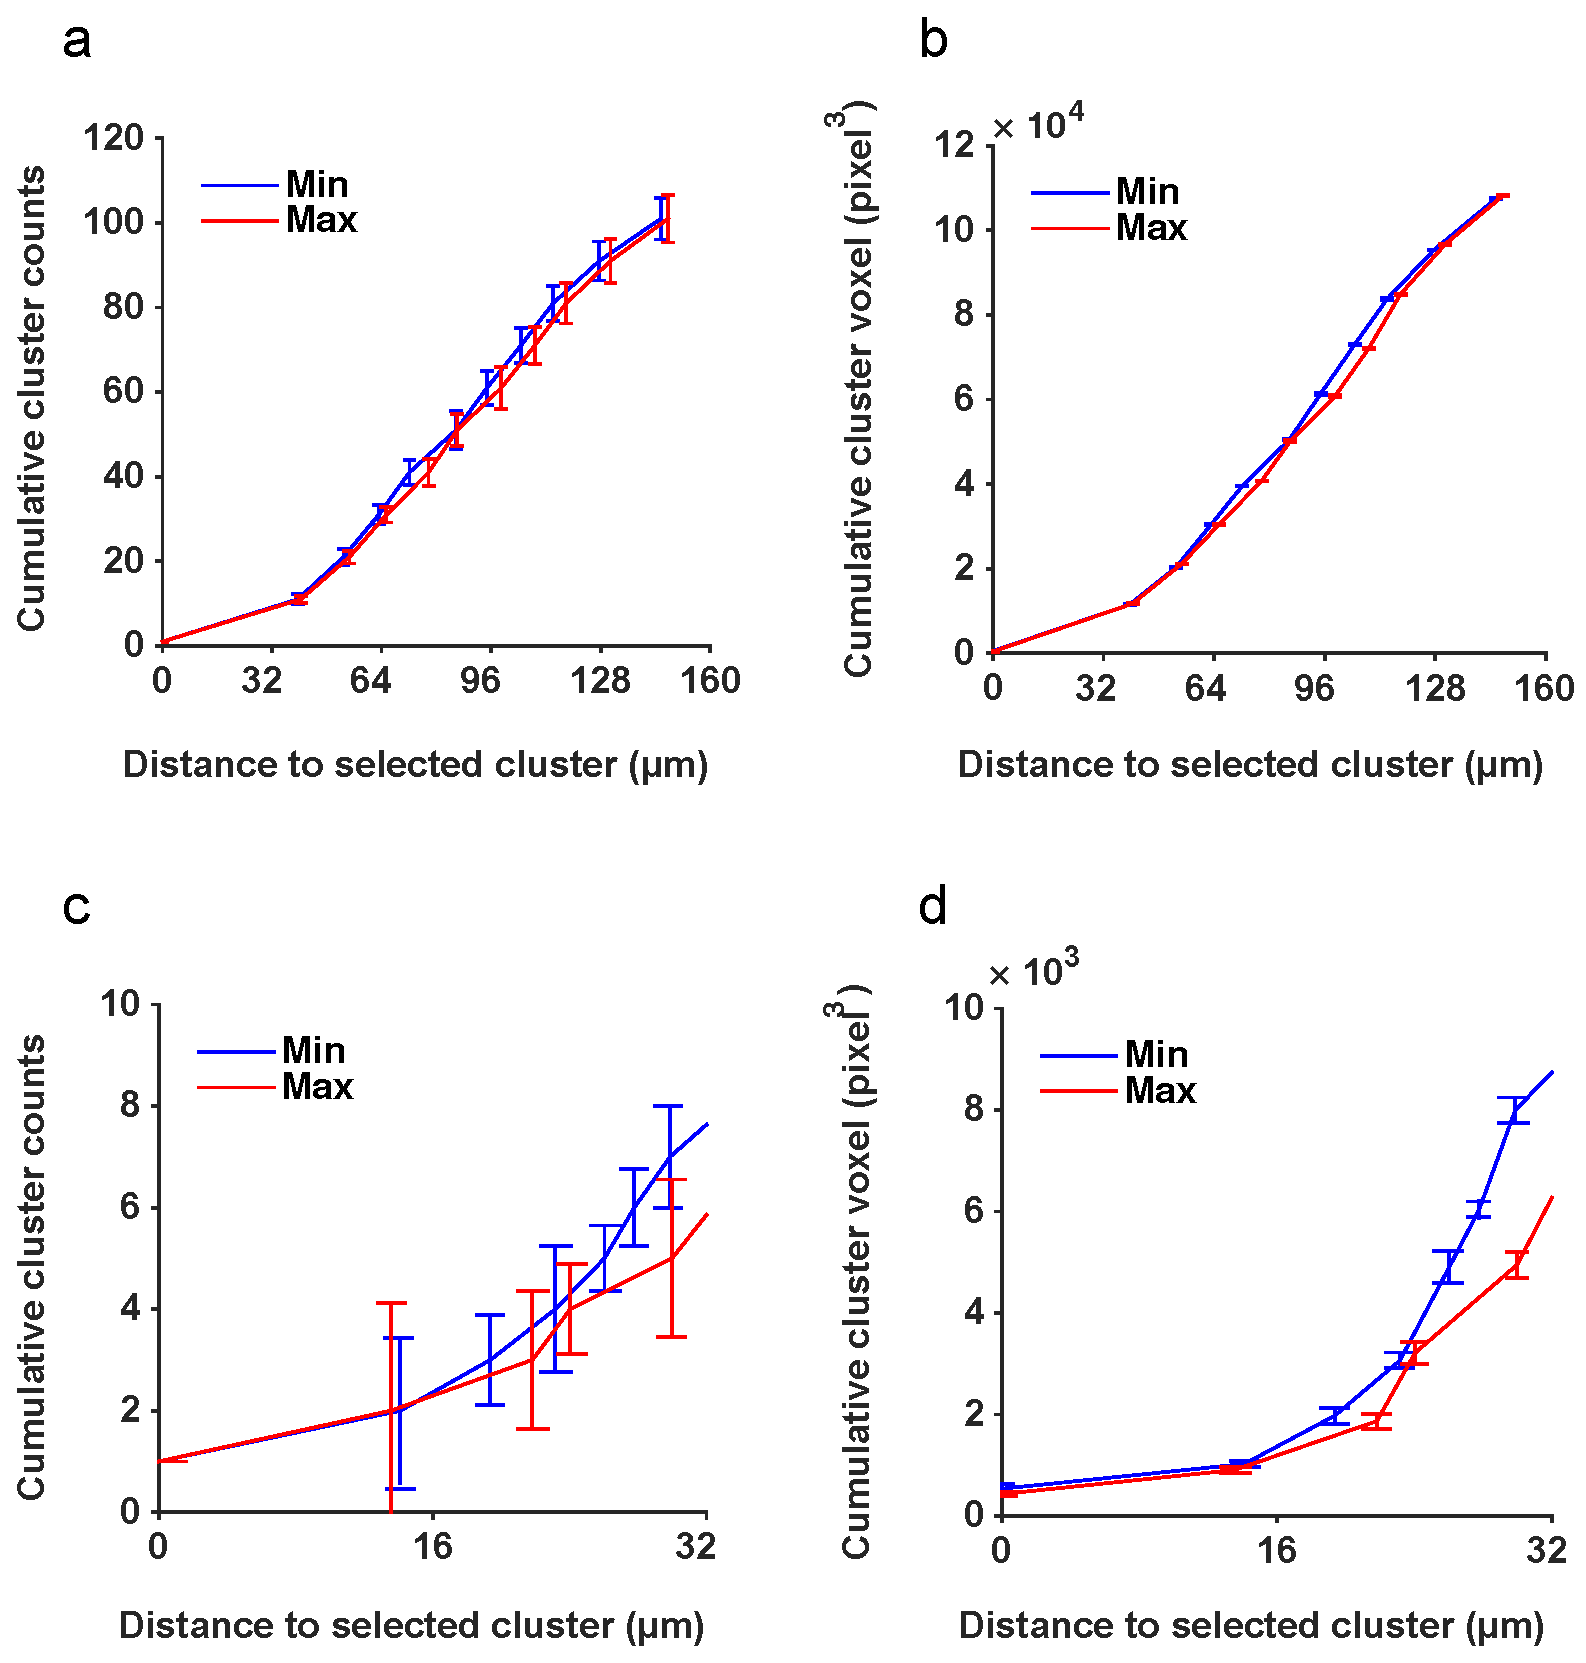
\includegraphics[keepaspectratio,width=0.8\textwidth]{./figures/10fM001_5ClusterZoomOut}
\caption[Cluster size and location correlation analysis]{Cluster size and location correlation analysis. Five reference clusters with the largest radii and five reference clusters with the smallest radii were chosen among clusters in one field of view (100+ clusters) of one MDA hydrogel sample. a) By zooming out from selected clusters, the number of other clusters encountered at successively greater distances was plotted. b) The total volume of other clusters encountered was plotted. c) and d) zoom-in views of a) and b) at 0 to 32 $\mu$m from reference clusters. We hypothesized that large clusters consume local resources and thus, would reduce the number and/or size of surrounding clusters. Although slight enhancements in the number and size of clusters surrounding the set of small reference clusters versus the set of large reference clusters exist, the effect is small. Error bars are SEM.}
\label{fig:ClusterCorrelation}
\end{figure}

\subsection{Analysis of reaction extent limitation and local competition among MDA clusters}
Based on additional studies, we concluded that a global auto-inhibition mechanism limits the growth of MDA clusters (Fig. \ref{fig:ClusterCorrelation}). We analyzed the variability in cluster number and DNA content around large and small reference clusters to test for local reagent competition among WGA reaction centers, finding little evidence for local competition. This observation is consistent with the high diffusion constants for enzymes, primers, and nucleotides measured in PEG hydrogels similar to ours \cite{Wu:2009ez,Weber:2009fe}. No specific limiting reagent was identified when reactants were supplemented individually (data not shown). The final reaction pH in our hydrogel reactions was measured to be 6.5 (initial pH = 7.5), which may limit cluster growth due to a global loss of polymerase activity at lower pH. Altogether, these data are consistent with density-dependent average size variation by global auto-inhibition, possibly by the pH drop. Variability of cluster size in a single experiment may result from variable initial template conformation, the degree of template denaturation, or local inhomogeneities in the hydrogel structure.

\section{Conclusion}
Here we tested the performance of \textit{virtual microfluidics} in-gel digital PCR and digital MDA amplification as an analytical method for molecular counting assays. \textit{Virtual microfluidics} enables high-throughput digital assays and preparative whole-genome amplification without microfabricated consumables or expensive instrumentation. Up to 20,000,000 analytes per $\mu$L could be accommodated due to the nature of the diffusion-restricted reaction and the continuous virtual chambers. Throughput could be increased by using a thinner gel with more surface area. Its excellent optical accessibility allows potential fluorescent labeling of rare sequences, which is a key in identifying rare targets in liquid biopsy applications. We expect \textit{virtual microfluidics} find applications as low-cost, highly accessible digital assay platforms that offer superior sensitivity and dynamic range. 

% The solid phase amplification environment also can contain potential infectious targets to minimize the handling of biohazardous materials for infectious disease diagnosis in the clinic and at the point-of-care diagnostic setting.

\section{Materials and Methods}
\subsection{PEG hydrogel cross-linking}
Hydrogel components, including 4-arm PEG acrylate (MW 10,000) and HS-PEG-SH (MW 3,400), were obtained from Laysan Bio. For every 25 $\mu$L of 10 \% (wt\slash v) cross-linked hydrogel, 1.6 mg of 4-arm PEG acrylate and 1.1 mg of HS-PEG-SH were dissolved in pH 7.4 PBS (Invitrogen). It was briefly vortexed and centrifuged to ensure mixing and it was allowed to sit on the bench for 10 min while the hydrogel components cross-linked through the reaction between the thiol and acrylate groups.
\subsection{In-gel digital PCR}
The primers (Table \ref{tab:ESprimerList}) used for PCR on purified \textlambda DNA (48 kbp, NEB) were ordered through IDT. A 25 $\mu$L hydrogel PCR reaction consisted of 2 U of VentR(exo-) polymerase (NEB), 1$\times$ ThermoPol Reaction Buffer (NEB), 0.4 mM dNTP (NEB), 1 $\mu$m Primers, 5 \% DMSO (Sigma), 0.5 mg\slash mL BSA (NEB), 1.6 mg 4-arm PEG acrylate in PBS, 1.1 mg HS-PEG-SH in PBS, and \textlambda DNA template (NEB) of various concentrations. The 25 $\mu$L above components were loaded in a 9 mm by 9 mm frame-seal chamber (Bio-rad). The following thermal protocol was ran on an MJ Research PTC--100 twin tower thermal cycler: 30 $^{\circ}$C for 30 min (gel polymerization), 98 $^{\circ}$C for 3 min; 98 $^{\circ}$C for 30 sec, 57 $^{\circ}$C for 30 sec, 72 $^{\circ}$C for 1 min for 40 to 60 cycles; 72 $^{\circ}$C for 5 min and hold at 4 $^{\circ}$C. The gel was stained with 500 nM SYTOX Orange nucleic acid dye (Invitrogen) (Fig. \ref{fig:dPCR_FS} and \ref{fig:dPCR_Calibration}).

\begin{figure}
\centering
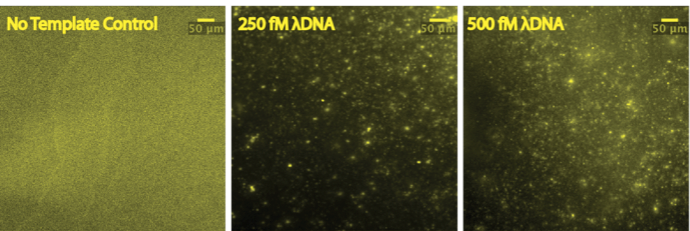
\includegraphics[keepaspectratio,width=1\textwidth]{./figures/dPCR_FrameSeal.png}
\caption[DNA amplification clusters from PCR in hydrogel in a frame-seal chamber.]{DNA amplification clusters from PCR in hydrogel in a frame-seal chamber. Each image is a z-axis max projection from a confocal tiff stack taken by a Zeiss spinning disk confocal microscope.}
\label{fig:dPCR_FS}
\end{figure}

\begin{figure}
\centering
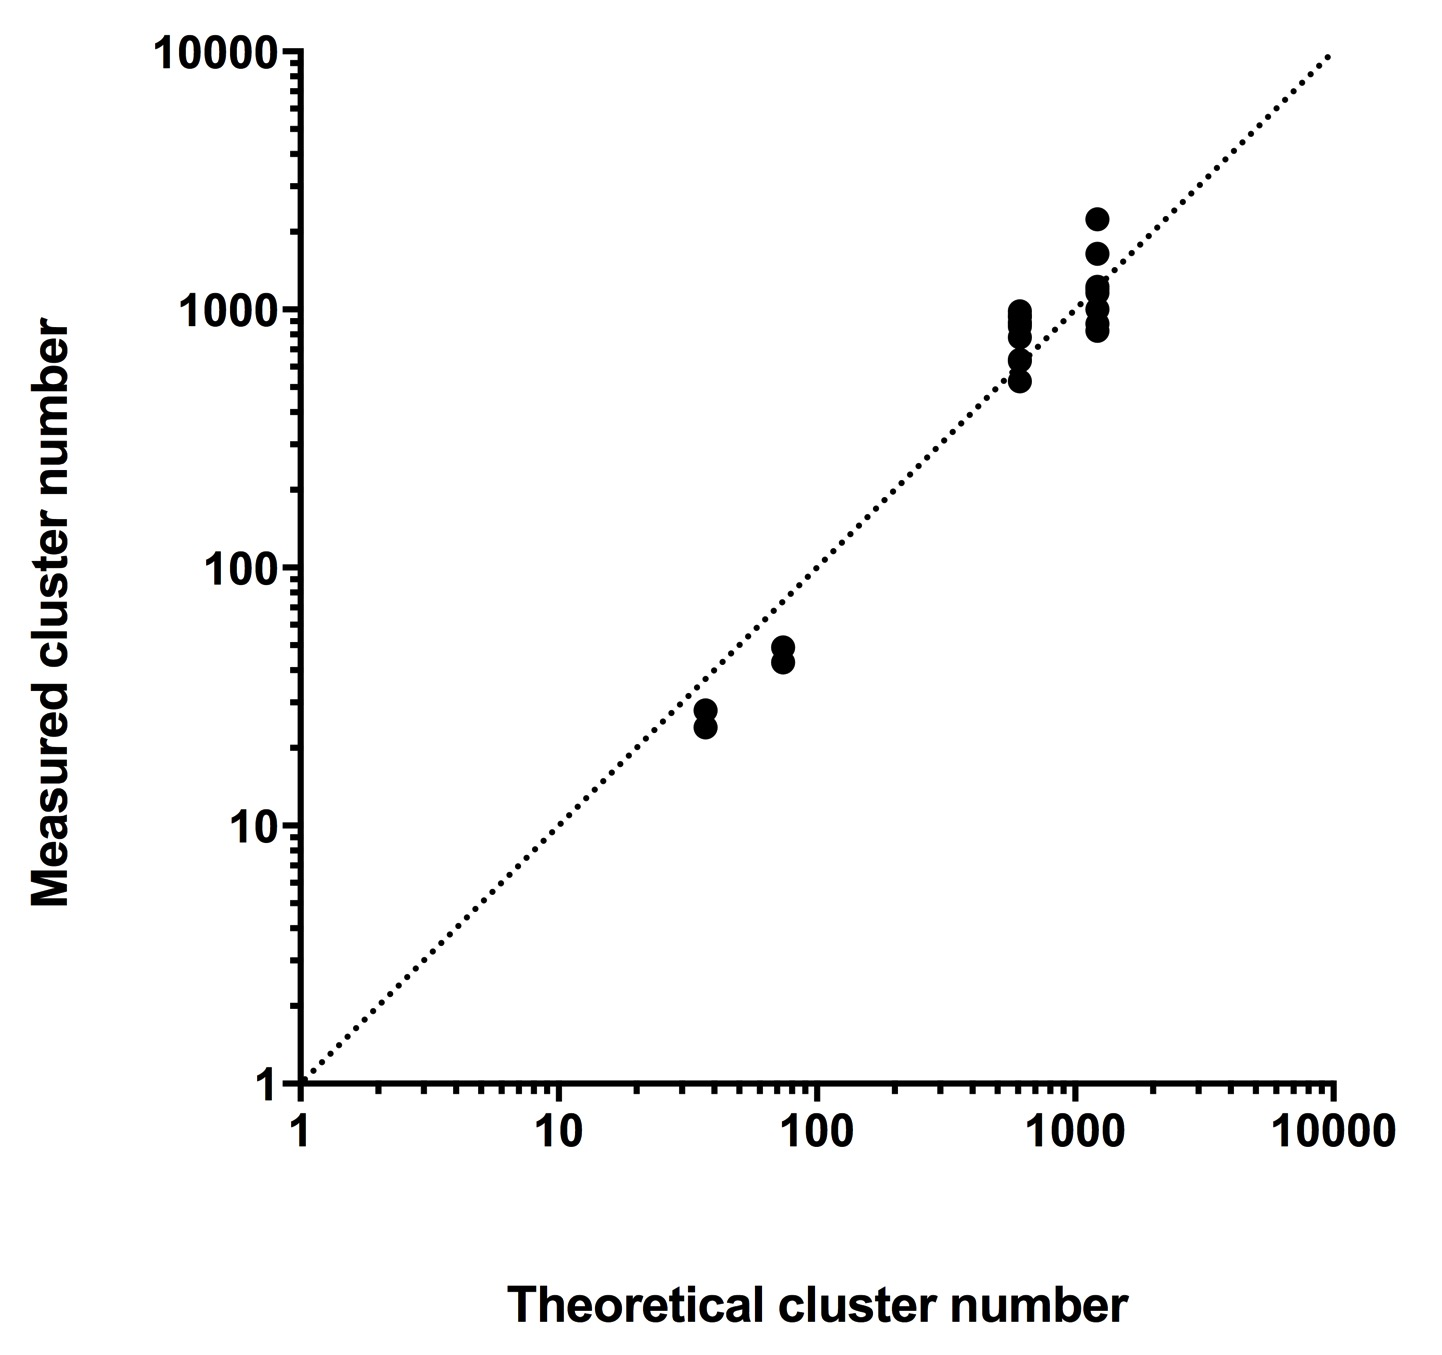
\includegraphics[keepaspectratio,width=0.5\textwidth]{./figures/SuppFig3.jpg}
\caption[Digital single-molecule PCR in hydrogel (Lambda phage DNA).]{Digital single-molecule PCR in hydrogel (Lambda phage DNA). Measured cluster number per field of view versus calculated cluster number based on template concentration. Reaction conditions are described in methods (PCR). The dotted line indicates the ideal situation when measured cluster number equals to the theoretical cluster number.}
\label{fig:dPCR_Calibration}
\end{figure}

\subsection{In-gel digital MDA}
A 25 $\mu$L hydrogel MDA reaction consisted of 0.5 $\mu$L of REPLI-g sc Polymerase (Qiagen), 1$\times$ $\Phi$29 buffer (NEB), 50 $\mu$m random hexamers (IDT; including two phosphorothioate bonds at 3' terminus), 2.5 \% DMSO, 0.4 mM dNTP, 0.5 mg\slash mL BSA, 500 nM SYTOX Orange (Invitrogen) and denatured \textlambda DNA. \textlambda DNA was denatured (using alkaline buffer ``D1'', Qiagen) and neutralized (buffer ``N1'', Qiagen) according to Qiagen REPLI-G sc kit protocol prior to hydrogel encapsulation. All MDA and gel components, except polymerase and SYTOX Orange dye, were UV treated for 30 min using the Stratalinker UV crosslinking instrument (Stratagene) to render contaminating background DNA incompetent for MDA. The 25 $\mu$L reaction mixture was loaded in a 9 mm by 9 mm frame-seal chamber (Bio-rad, about 300 $\mu$m in height). The gel was sealed in the chamber with a plastic cover and maintained at 30 $^{\circ}$C for 8 hours or longer in the MJ Research PTC--100 twin tower thermal cycler. After the reaction, we imaged the gel using Nikon ECLIPSE Ti inverted microscope or Nikon ultra-fast laser scanning confocal microscope (MIT Koch Institute Microscopy Core Facility) (Fig. \ref{fig:dMDA_Quant}a).
\subsection{In-gel real-time dMDA}
MDA hydrogel reactions were set up as described above and conducted at room temperature for 6 hours on a Nikon ECLIPSE Ti Epi-Fluorescence Microscope excited with a Lumencor Spectra X light engine (Lumencor) with fluorescent emissions filtered through a SpGold filter (Semrock) (Fig. \ref{fig:dMDA_Quant}b). MATLAB was used to capture time-lapse image stacks through a Nikon 20$\times$\slash 0.4 NA objective and Hamamatsu C11440 camera with 15 min intervals, 100 ms exposure time, and 10 \% Lumencor excitation power. All samples were stained with 500 nM SYTOX Orange. Each \textit{E. coli.} MDA cluster or mammalian cell image stack was cropped and processed as described below.


% \begin{figure}
% \centering
% 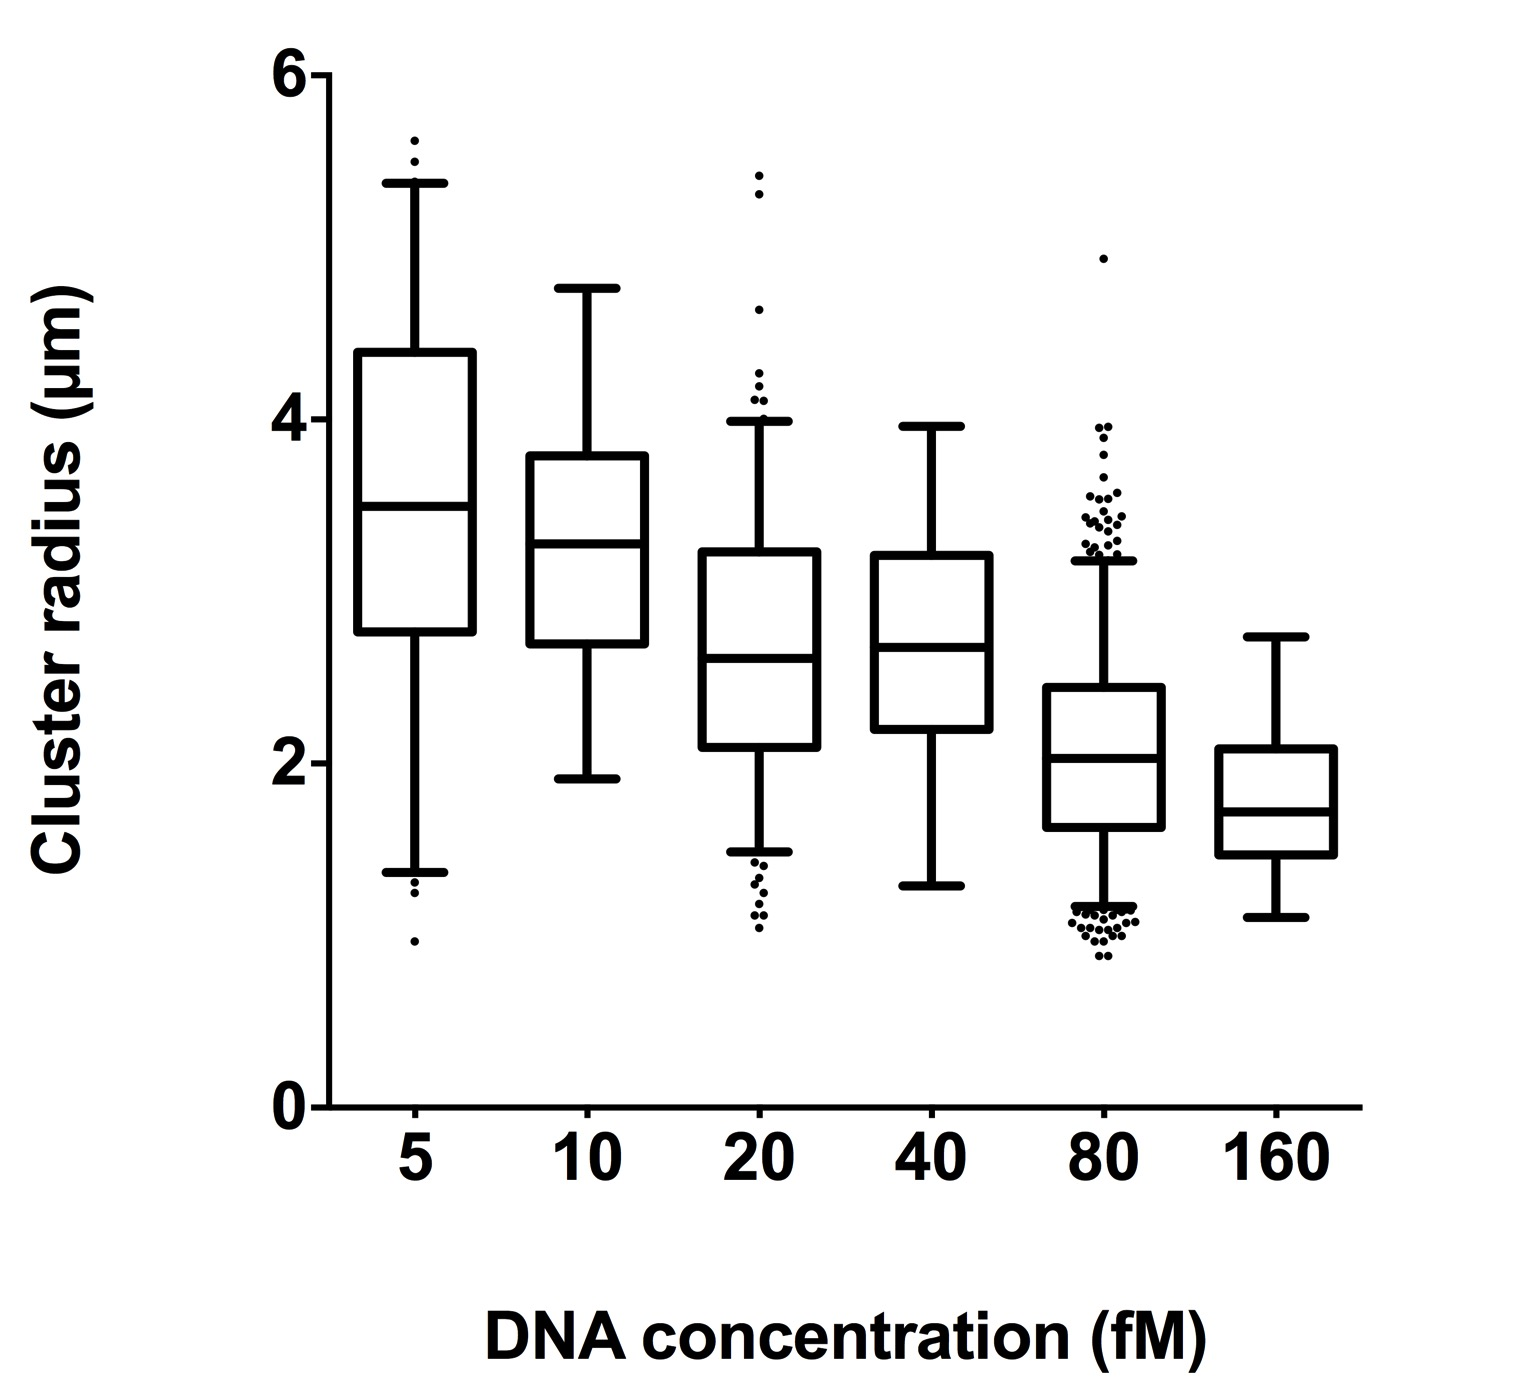
\includegraphics[keepaspectratio,width=0.5\textwidth]{./figures/SuppFig4.jpg}
% \caption[MDA cluster size decreases with increasing DNA template concentration]{MDA cluster size decreases with increasing DNA template concentration with the same gel condition. Data is shown as 5 \% - 95 \% box plot with outliers scattered and the centerline as the median. (n = 2 fields of view at each concentration, number of clusters for each field of view is: n = 43, 62, 89, 88, 191, 167, 321, 305, 478, 542, 711, 833).}
% \label{fig:dMDA_Quant}
% \end{figure}

% \begin{figure}
% \centering
% 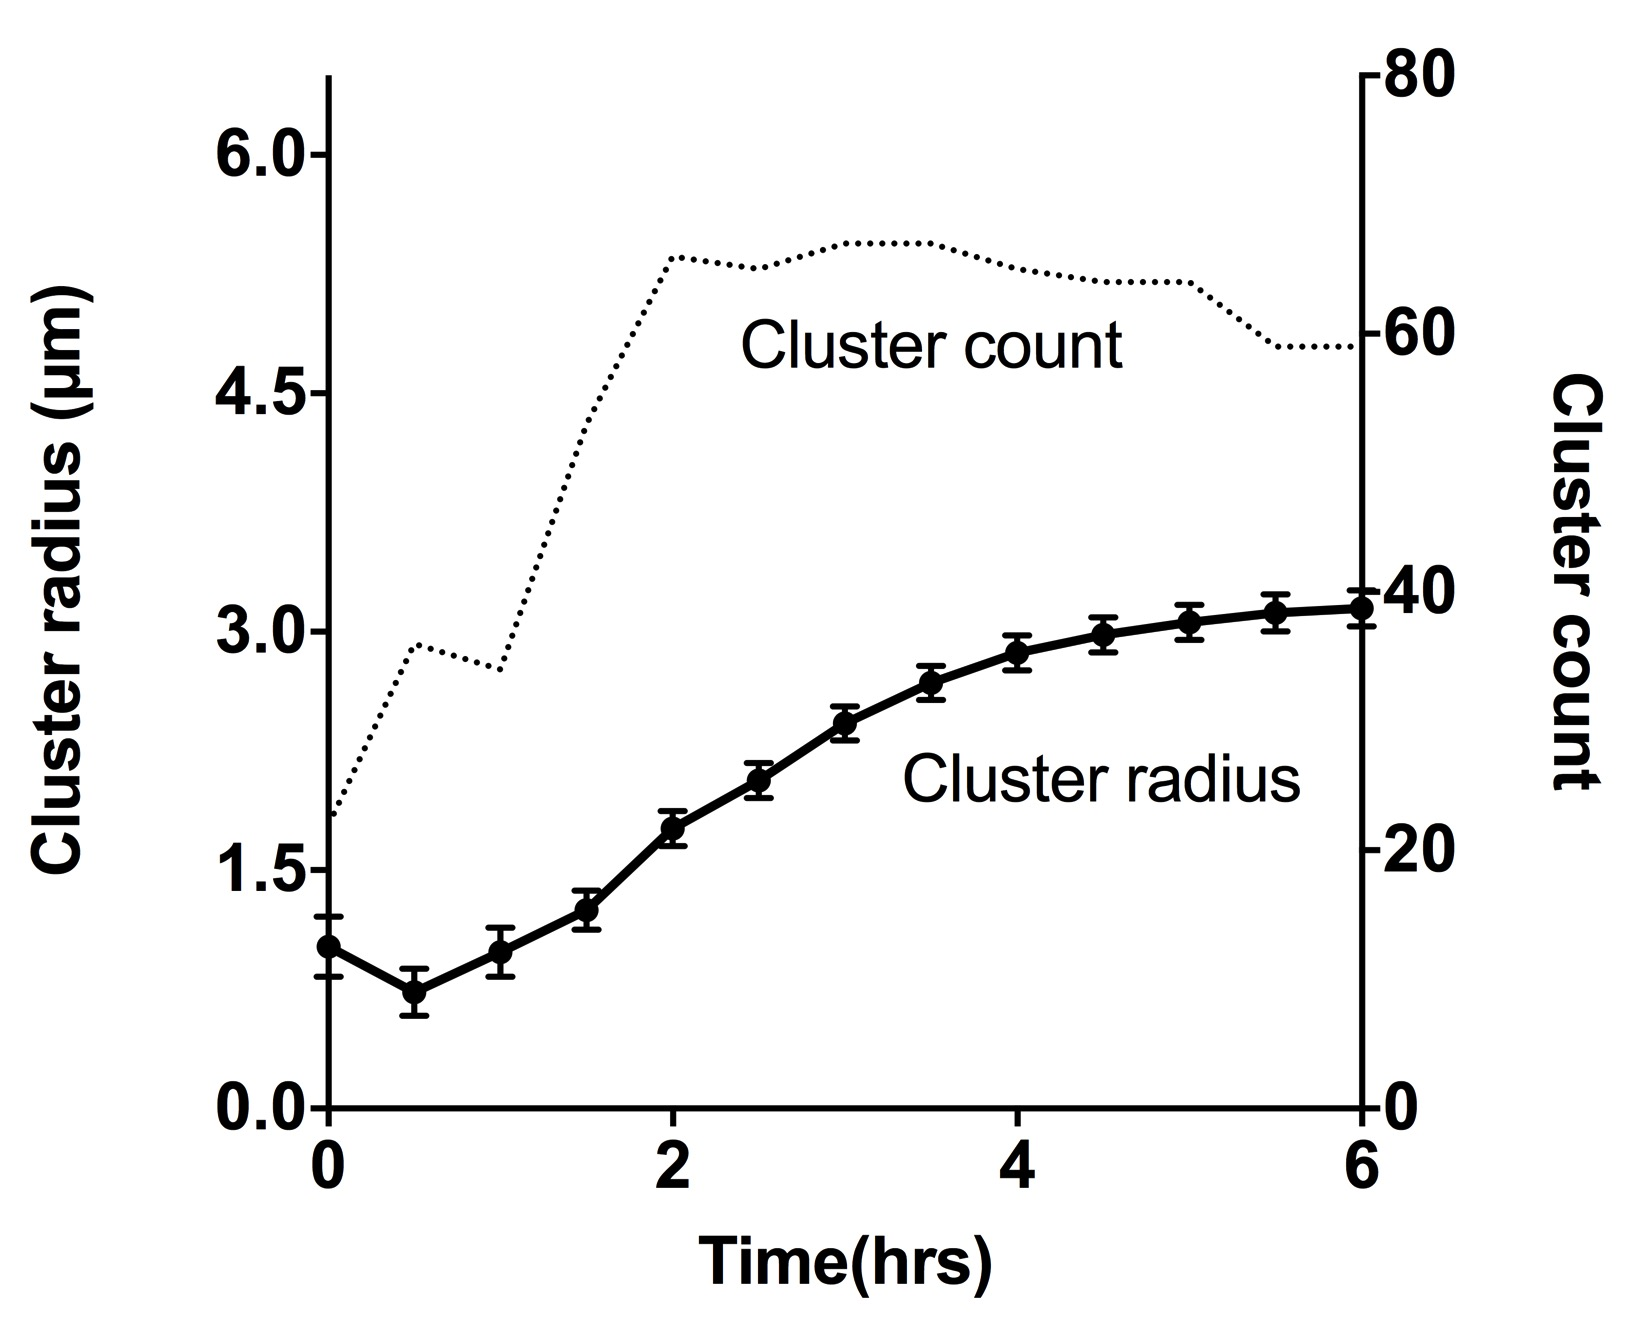
\includegraphics[keepaspectratio,width=0.5\textwidth]{./figures/SuppFig1.jpg}
% \caption[Real time dMDA for quantification of cluster growth and count with time.]{Real time dMDA for quantification of cluster growth and count with time. The cluster radius curve shows mean radius $\pm$ SEM. The zero time point cluster count and radius data points reflect the properties of fluorescent contaminants.}
% \label{fig:dMDA_Quanttime}
% \end{figure}

% \begin{figure}
% \centering
% 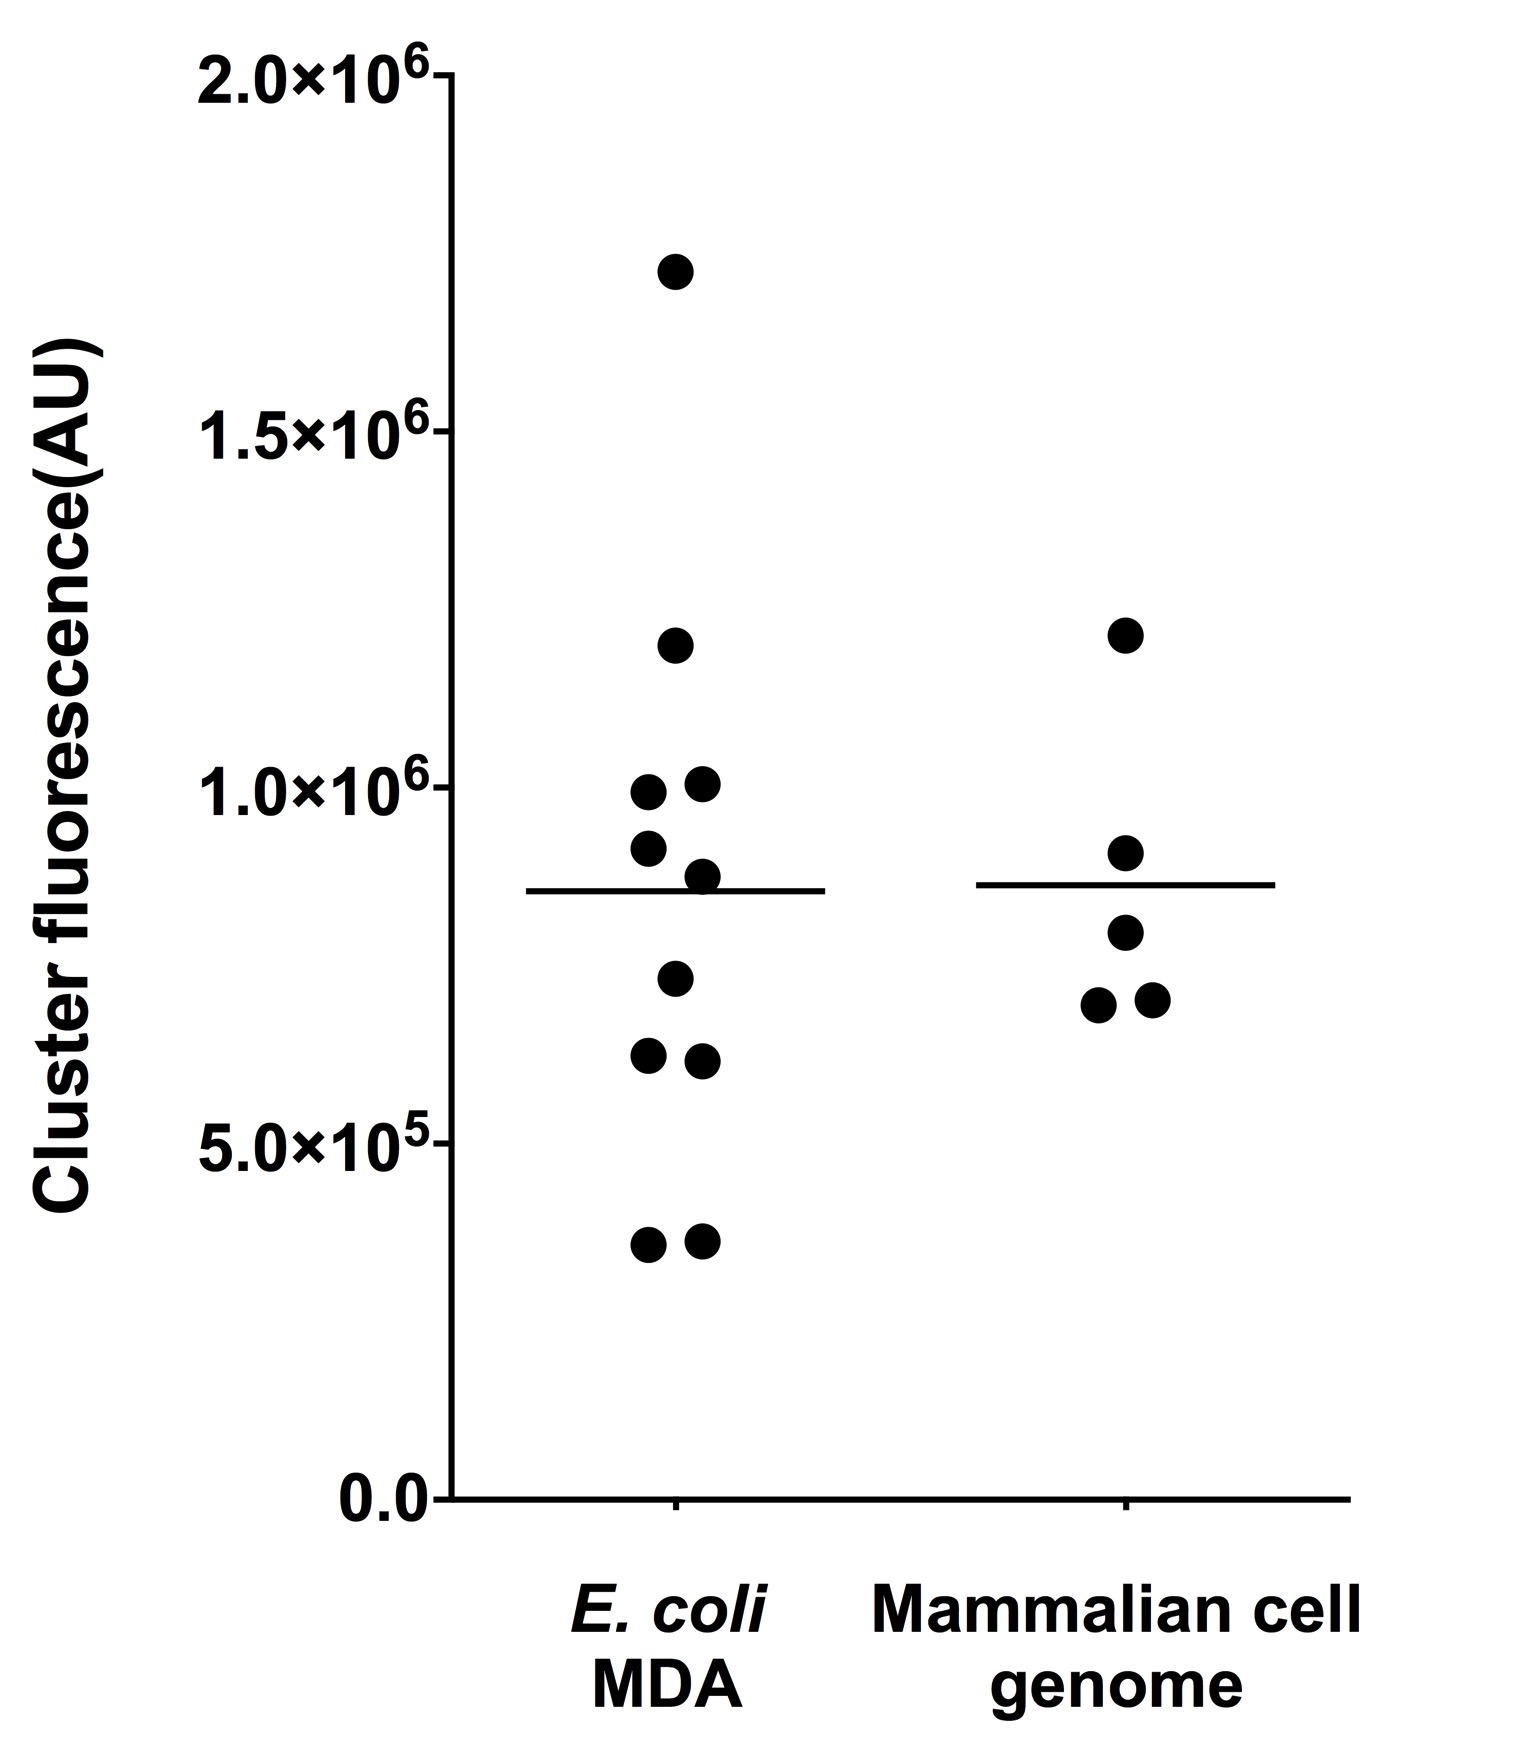
\includegraphics[keepaspectratio,width=0.5\textwidth]{./figures/SuppFig2.jpg}
% \caption[\textit{E. coli} MDA cluster quantification.]{\textit{E. coli} MDA cluster quantification. \textit{E. coli} MDA cluster's DNA content was calibrated against (unamplified) hydrogel-embedded mammalian cells (HEK 293) by comparing SYTOX Orange fluorescence intensities. DNA content in individual product clusters and mammalian cells was approximated by integrating pixel intensities under the same hydrogel and staining conditions. The observed integrated fluorescence was comparable across MDA product clusters and unamplified mammalian cells, leading us to conclude that the average DNA content per MDA product cluster was approximately equal to the average DNA content of an unsynchronized mammalian cell population, or on the order of 10 pg. The centerline represents the mean value.}
% \label{fig:SuppFig2}
% \end{figure}

\subsection{Image acquisition and analysis}
Z-stack images were taken by Nikon ultra-fast laser scanning confocal microscope with pinhole = 1.2, HV = 112, offset = 0, laser wavelength = 561 nm, laser power = 1.3 to 1.5, using a 20$\times$ objective on Galvano mode. Acquisition speed was 1 frame\slash sec and z step size was 0.95 $\mu$m. On the inverted microscope, z-stack images were taken with the exposure time 100 ms, Lumencor excitation power 10 \%, binning size 2 and z step size 10 $\mu$m. Both z Stacks were first processed into max intensity projections in FIJI(FIJI is just image J). Max projection tif files were then loaded into MATLAB. The background was obtained by applying a Gaussian filter of hsize 200 and sigma 50. All max projections were background-subtracted and thresholded at 2$\times$ \textendash 2.5$\times$ standard deviations above the mean intensity. Cluster count, cluster area (radius), and cluster mean intensity were obtained with the bwconncomp and regionprops functions (Fig. \ref{fig:dMDA_MammalianEcoliCluster}).

\begin{figure}
\centering

\includegraphics[keepaspectratio,width=1\textwidth]{./figures/MammalianEcoliCluster}
\caption[Imaging analysis for a \textit{E. coli} MDA cluster and a mammalian genome]{Imaging analysis for a \textit{E. coli} MDA cluster and a mammalian genome. a) The \textit{E. coli} MDA cluster and the mammalian genome were imaged with a Nikon confocal microscope. The cluster radius of each were ploted. b) The mean fluorescence of each stack was plotted for the \textit{E. coli} MDA cluster and the mammalian genome.}
\label{fig:dMDA_MammalianEcoliCluster}
\end{figure}
\chapter{\textbf{\textit{Virtual Microfluidics}} enables high-quality single-cell sequencing from a mixed population of cultured bacteria and the human gut microbiome}

This thesis chapter is reproduced from a previously published paper, Xu \textit{et al.}, Nature Methods, 2016 \cite{Xu:2016wt}. Experiments and data analysis on the cultured bacteria were performed by Liyi Xu. Ilana Brito and Liyi Xu conducted the data analysis of the gut microbiome data.

% \section{Abstract}
% We applied in-gel digital multiple displacement amplification (dMDA) to cultured bacteria and demonstrated whole-genome sequencing of single-cell MDA products with excellent coverage uniformity and markedly reduced chimerism compared with liquid MDA reactions. We demonstrated single-cell sequencing on human gut microbiome samples and obtained 117 pure single draft genomes that enabled the identification of more than 10,000 horizontally transferred genes that have unique population-specific and individual-specific features.

\section{Introduction}
In the burgeoning field of single cell analysis \cite{Blainey:2013hn}, high-throughput and high-fidelity whole-genome \cite{Fu:2015gl,Zhang:2006hq,Raghunathan:2005fg} and whole-transcriptome amplification (WGA and WTA) reactions are needed to produce sufficient material for sequence library construction to support the discovery and validation of new genomes \cite{Marshall:2012jz,Pamp:2012cj,Hess:2011gu}, as well as the analysis of genomic and functional heterogeneity \cite{Wang:2012bb,Fu:2015gl,Pamp:2012cj}.

A variety of approaches have been explored for compartmentalization across a large number of discrete reactors, including SBS plates \cite{Zhang:2006hq}, high-density microfluidic arrays \cite{Love:2013hf}, engineered lab-on-chip systems \cite{Thorsen:2002dn,Landry:2013dh,deBourcy:2014ji,Marcy:2007ip}, and multi-phase micro-droplet systems \cite{Fu:2015gl,Thorsen:2001td,Hindson:2011fg,Morinishi:2015jx}. However, they require complex instrumentation and microfabricated consumables that hinder broad deployment. An ideal platform should resist external contaminants and cross-compartment mixing, exhibit high throughput in small reaction volumes, be stable under temperature change, allow optical access, and allow facile addition and removal of reagents and samples. Finally, it should generate high-quality amplified products and minimize biases and artifacts, such as chimeric fragments commonly formed in PCR, WGA and WTA, that can severely impact single-cell sequencing results. 

Building on my work in Chapter 2 on characterizing \textit{virtual microfluidics} for DNA digital quantification, I further developed the technology for single-cell sequencing. 

\section{Results and Discussion}
\subsection{In-gel single \textit{E. coli} MDA}
We applied digital MDA at the single-cell level using the \textit{virtual microfluidics} system. Individual log-phase \textit{Escherichia coli} could be identified in the hydrogel by fluorescence microscopy (Fig. \ref{fig:EcoliMDA}). We lysed the embedded cells by heat treatment and carried out MDA on the denatured genomic DNA, observing the appearance of MDA clusters at the reaction endpoint.

\begin{figure}
\centering
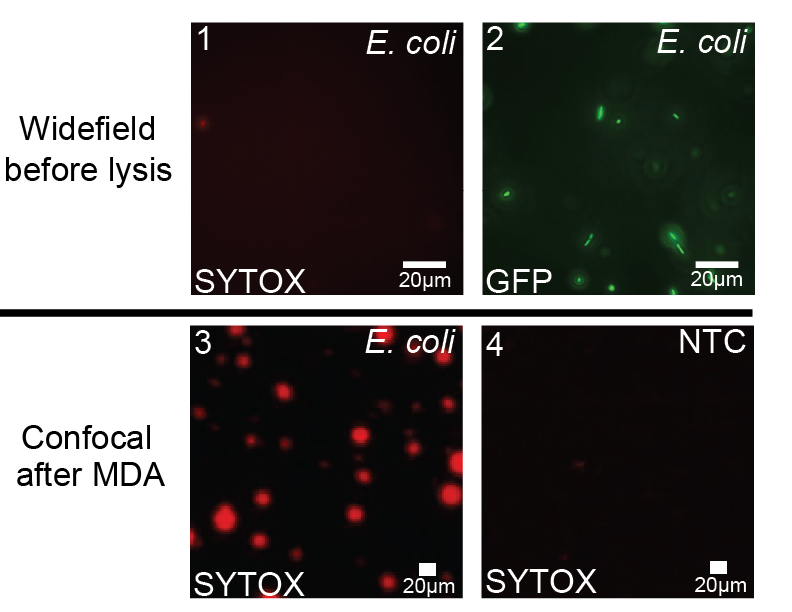
\includegraphics[keepaspectratio,width=0.5\textwidth]{./figures/Thesis-22.png}
\caption[Single-cell MDA on \textit{Escherichia coli}]{Single-cell MDA on \textit{Escherichia coli}. Hydrogel-encapsulated \textit{E. coli}  express GFP and exclude SYTOX Orange before lysis. SYTOX Orange staining reveals product clusters after MDA. Top images are from the same field of view. NTC, MDA control lacking \textit{E. coli}.}
\label{fig:EcoliMDA}
\end{figure}

\subsection{In-gel single-microbe MDA - cultured \textit{E. coli}  and \textit{S. aureus}}
Next, we tested the potential of \textit{virtual microfluidics} to support single-cell shotgun genome sequencing (Fig. \ref{fig:ESMDA}). We mixed log-phase \textit{Escherichia coli} (BL21) and \textit{Staphylococcus aureus subsp. aureus} (RN6390\slash 8325) strains at about 200,000 cells\slash mL and embedded the cells in a 300 micron thick PEG hydrogel. We used a mixed-input approach to ensure sensitive identification of any cross-contamination among single-cell samples and any contamination of single cell samples from other sources (including \textit{E. coli}  DNA contamination). The embedded cells were lysed by enzymatic and heat treatment, and MDA reagents were introduced by diffusion into the gel. Eighty sub-samples from the gel (of 60 nL each) were recovered manually in a grid pattern as indicated in Fig. \ref{fig:ESMDA}a Each punch sample was re-amplified to $10^{9}$ - $10^{10}$ overall fold-amplification in a second-round 20 $\mu$L liquid MDA reaction. Real-time PCR (QPCR) assays for \textit{E. coli}  and \textit{S. aureus}  genome sequences were applied to diluted aliquots from each sample (Table \ref{tab:QpcrHydrogel} and \ref{tab:ESprimerList}). The QPCR results were well-approximated by a random cell dispersion model.

\begin{table}
\centering 
\caption{QPCR characterization of hydrogel punches}
\label{tab:QpcrHydrogel}
\begin{adjustbox}{max width=0.7\textwidth}
\begin{tabular}{c||c} 

\hline 
Total hydrogel punches & 80 \\ 
\hline
\textit{E. coli} positive punches & 7  \\
\hline
\textit{S. aureus} positive punches & 36 \\
\hline
Double positive & 7 \\
\hline
Double negative & 30 \\
\hline
\end{tabular}
\end{adjustbox}
\end{table}

\begin{figure}
\centering
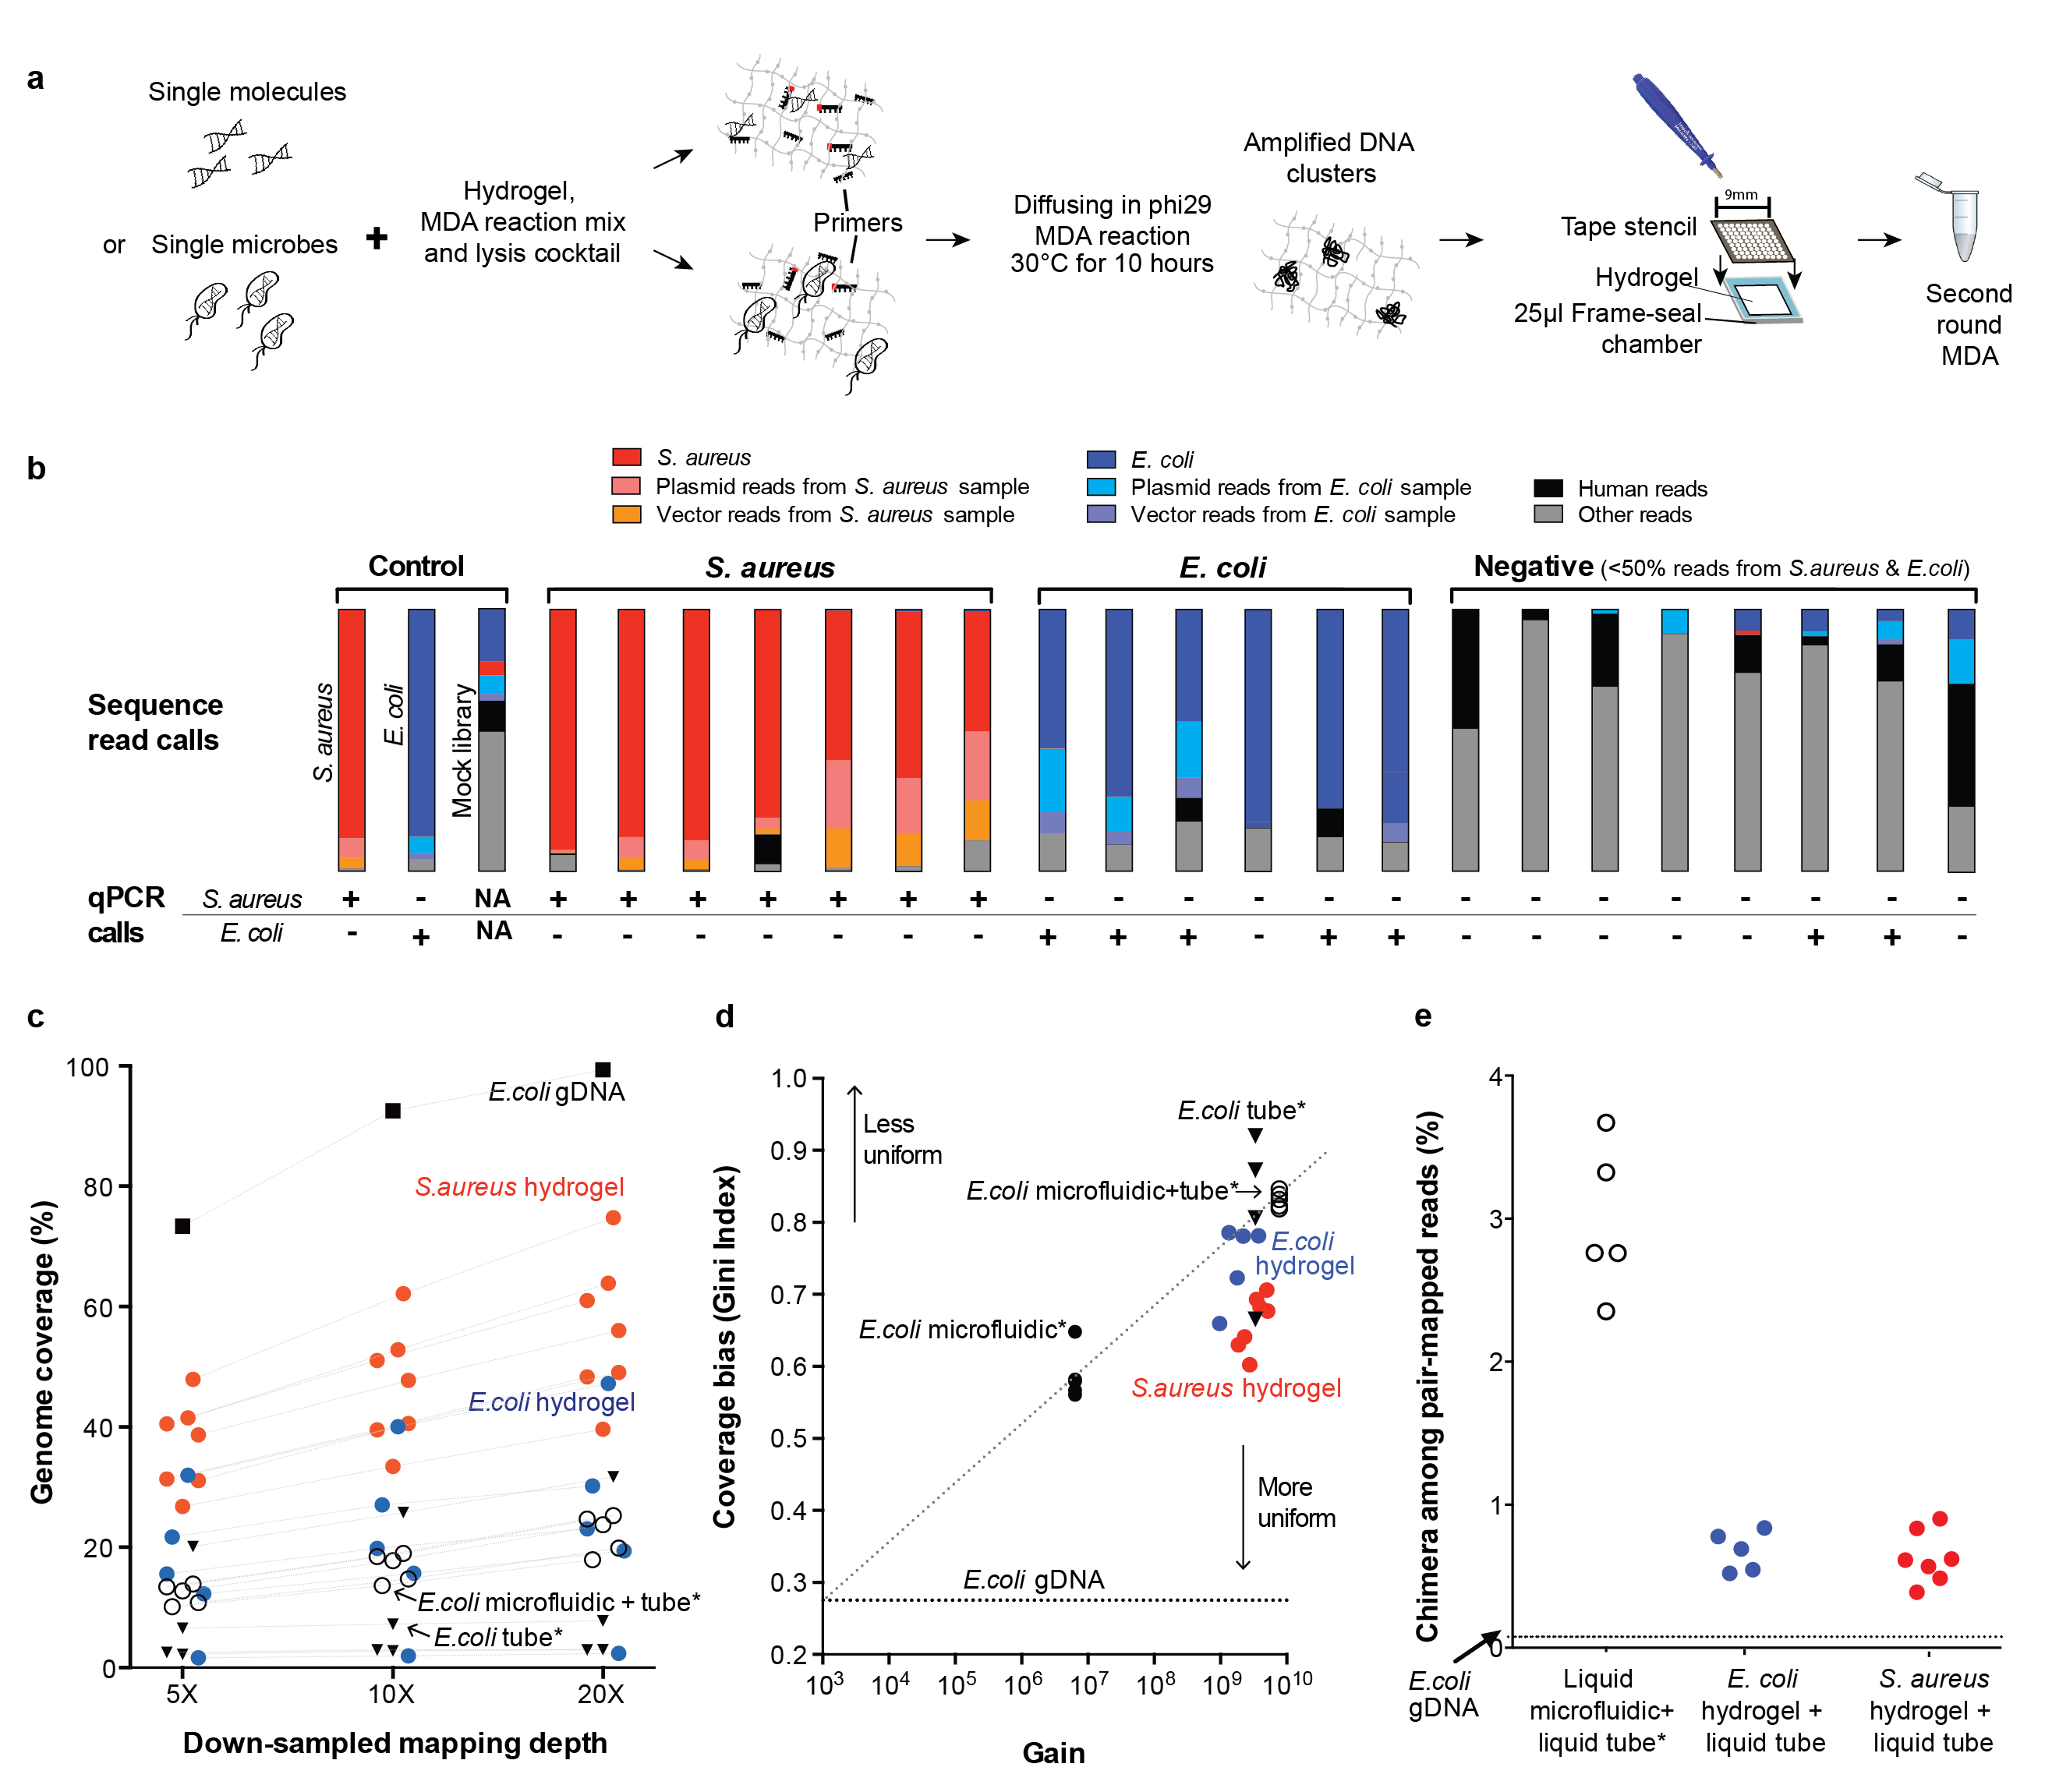
\includegraphics[keepaspectratio,width=0.95\textwidth]{./figures/Thesis-16.png}
\caption[Single-cell whole genome sequencing from \textit{E. coli} and \textit{S. aureus} hydrogel WGA samples.]{Single-cell whole genome sequencing from \textit{E. coli} and \textit{S. aureus} hydrogel WGA samples. (a) \textit{Virtual microfluidics} WGA workflow. (b) Sequence read classification using BLAST against the corresponding databases. The samples were ordered based on the ratio of \textit{S. aureus}  to \textit{E. coli}  reads from shotgun sequencing and the fraction of reads not from \textit{S. aureus}  or \textit{E. coli}. Two negative samples are classified as false positive PCR calls. Positive \textit{S. aureus}  and \textit{E. coli}  samples with matching PCR calls are included in downstream analyses. (c) Genome coverage in \textit{S. aureus}  and \textit{E. coli}  hydrogel punch samples compared with published single-cell \textit{E. coli} data produced using conventional liquid MDA reactions*. One \textit{E. coli}  outlier library showed extremely poor genome coverage. This library had low complexity (37\% duplicate reads), which points to poor library quality rather than MDA as the cause for low genome coverage. All samples were randomly down-sampled based on mapped reads and bootstrapped 10 times; error in all cases was smaller than the symbols plotted. (d) Coverage distribution bias. Gini Index (derived from Lorenz curve) reports the genome coverage bias of single-cell \textit{E. coli}  and \textit{S. aureus}  punches compared to the same published liquid-MDA single-cell \textit{E. coli}  data as a function of amplification gain. (e) Chimera frequency in the virtual microfluidics samples is significantly reduced versus published \textit{E. coli}  data produced using standard liquid MDA reactions. $\Astericks$ Indicates liquid MDA data from de Bourcy \textit{et al.} 2014.}
\label{fig:ESMDA}
\end{figure}

We sequenced Illumina short-insert libraries produced from randomly selected punch samples and positive-control gDNA samples (MiSeq v2 500 cycles). Quality-filtered reads were then mapped to \textit{de novo} assemblies of the positive-control gDNA datasets and sequence databases (Table \ref{tab:MapStatES}, Table \ref{tab:deNovoAssemblyES}). The positive punch samples showed strong enrichment (Fig. \ref{fig:ESMDA}b) for reads mapping to the expected reference genome (Fig. \ref{fig:MappingES}) while the negative punch samples showed enrichment for human reads, reads with poor mapping quality, and \textit{E. coli} (possibly contaminants from the reagents and\slash or laboratory environment), and were similar to the results from a mock library (Table \ref{tab:BlastReadsES}). The lack of \textit{E. coli}  and \textit{S. aureus} cross-contamination in the positive punch samples indicates that \textit{virtual microfluidics} can resolve single-cell amplification products.

\begin{table}
\caption{Sequence read classification of "other reads"}
\begin{center}
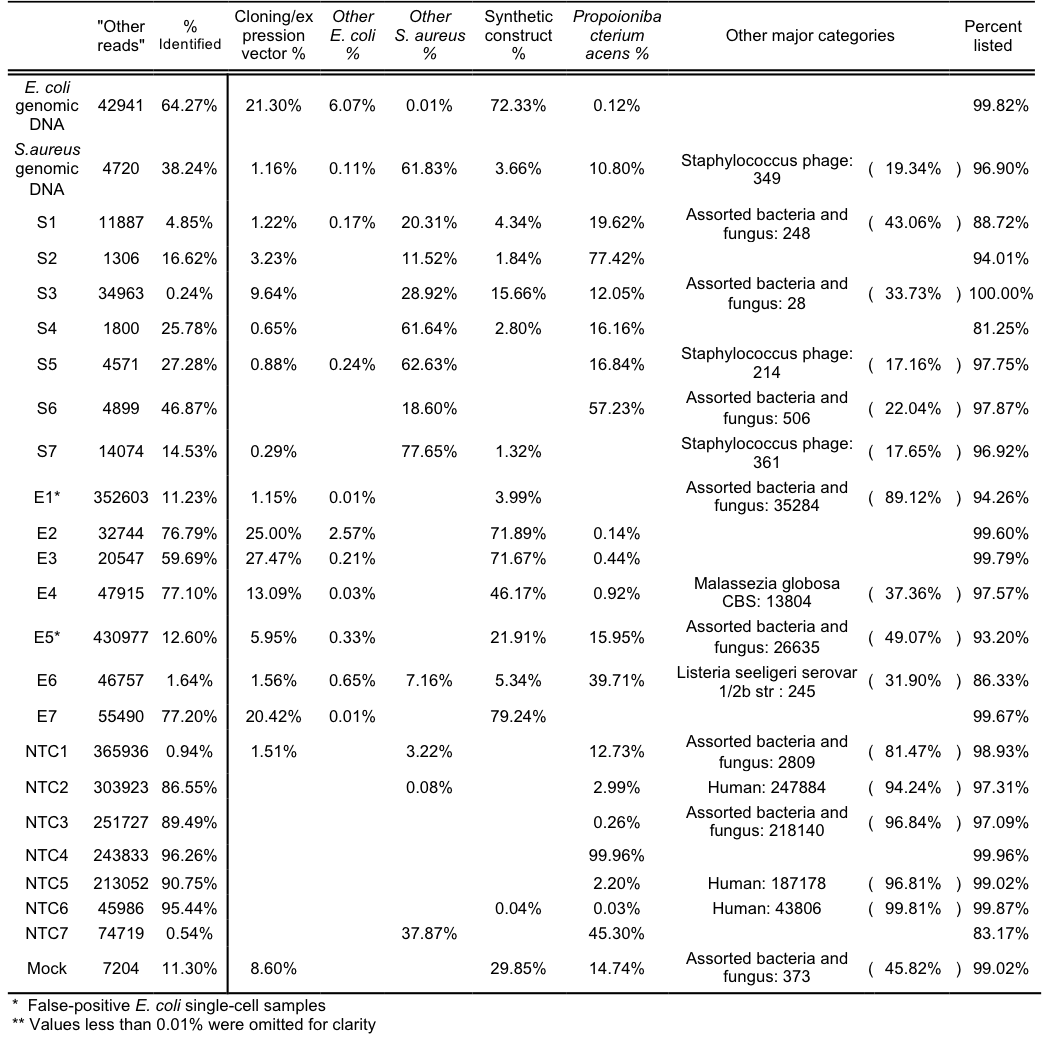
\includegraphics[width=\textwidth]{./figures/OtherReadsClassificationES}
\end{center}
\label{tab:BlastReadsES}
\end{table}

At 20$\times$ mean coverage (Table \ref{tab:DownsamplingESD} in methods), approximately 30\% of the \textit{E. coli}  genome and about 60\% of the \textit{S. aureus}  genome were covered in each single-cell sample (Fig. \ref{fig:ESMDA}c). The coverage values for \textit{E. coli}  are in-line with typical single microbe genome sequencing at similar sequencing effort \cite{deBourcy:2014ji,Woyke:2011eg}. The superior coverage performance in \textit{S. aureus}  may be attributable to the lower GC content of \textit{S. aureus}  (33\%) compared with \textit{E. coli}  (51\%), better accessibility (deproteination) of the genome after lysis, and\slash or higher average genome equivalents per cell in \textit{S. aureus} resulting from cell cycle dynamics.

To rigorously evaluate sequence coverage distribution, we calculated the Gini Index (a measure of inequity ranging from 0 to 1) for each of our single-cell datasets and previously published single-cell \textit{E. coli} liquid MDA datasets for which raw read data were available and fold-amplification was known (Fig. \ref{fig:ESMDA}d). The coverage uniformity in our single-cell punch samples compares favorably with published single-cell datasets at similar amplification gain.

\begin{figure}
\centering
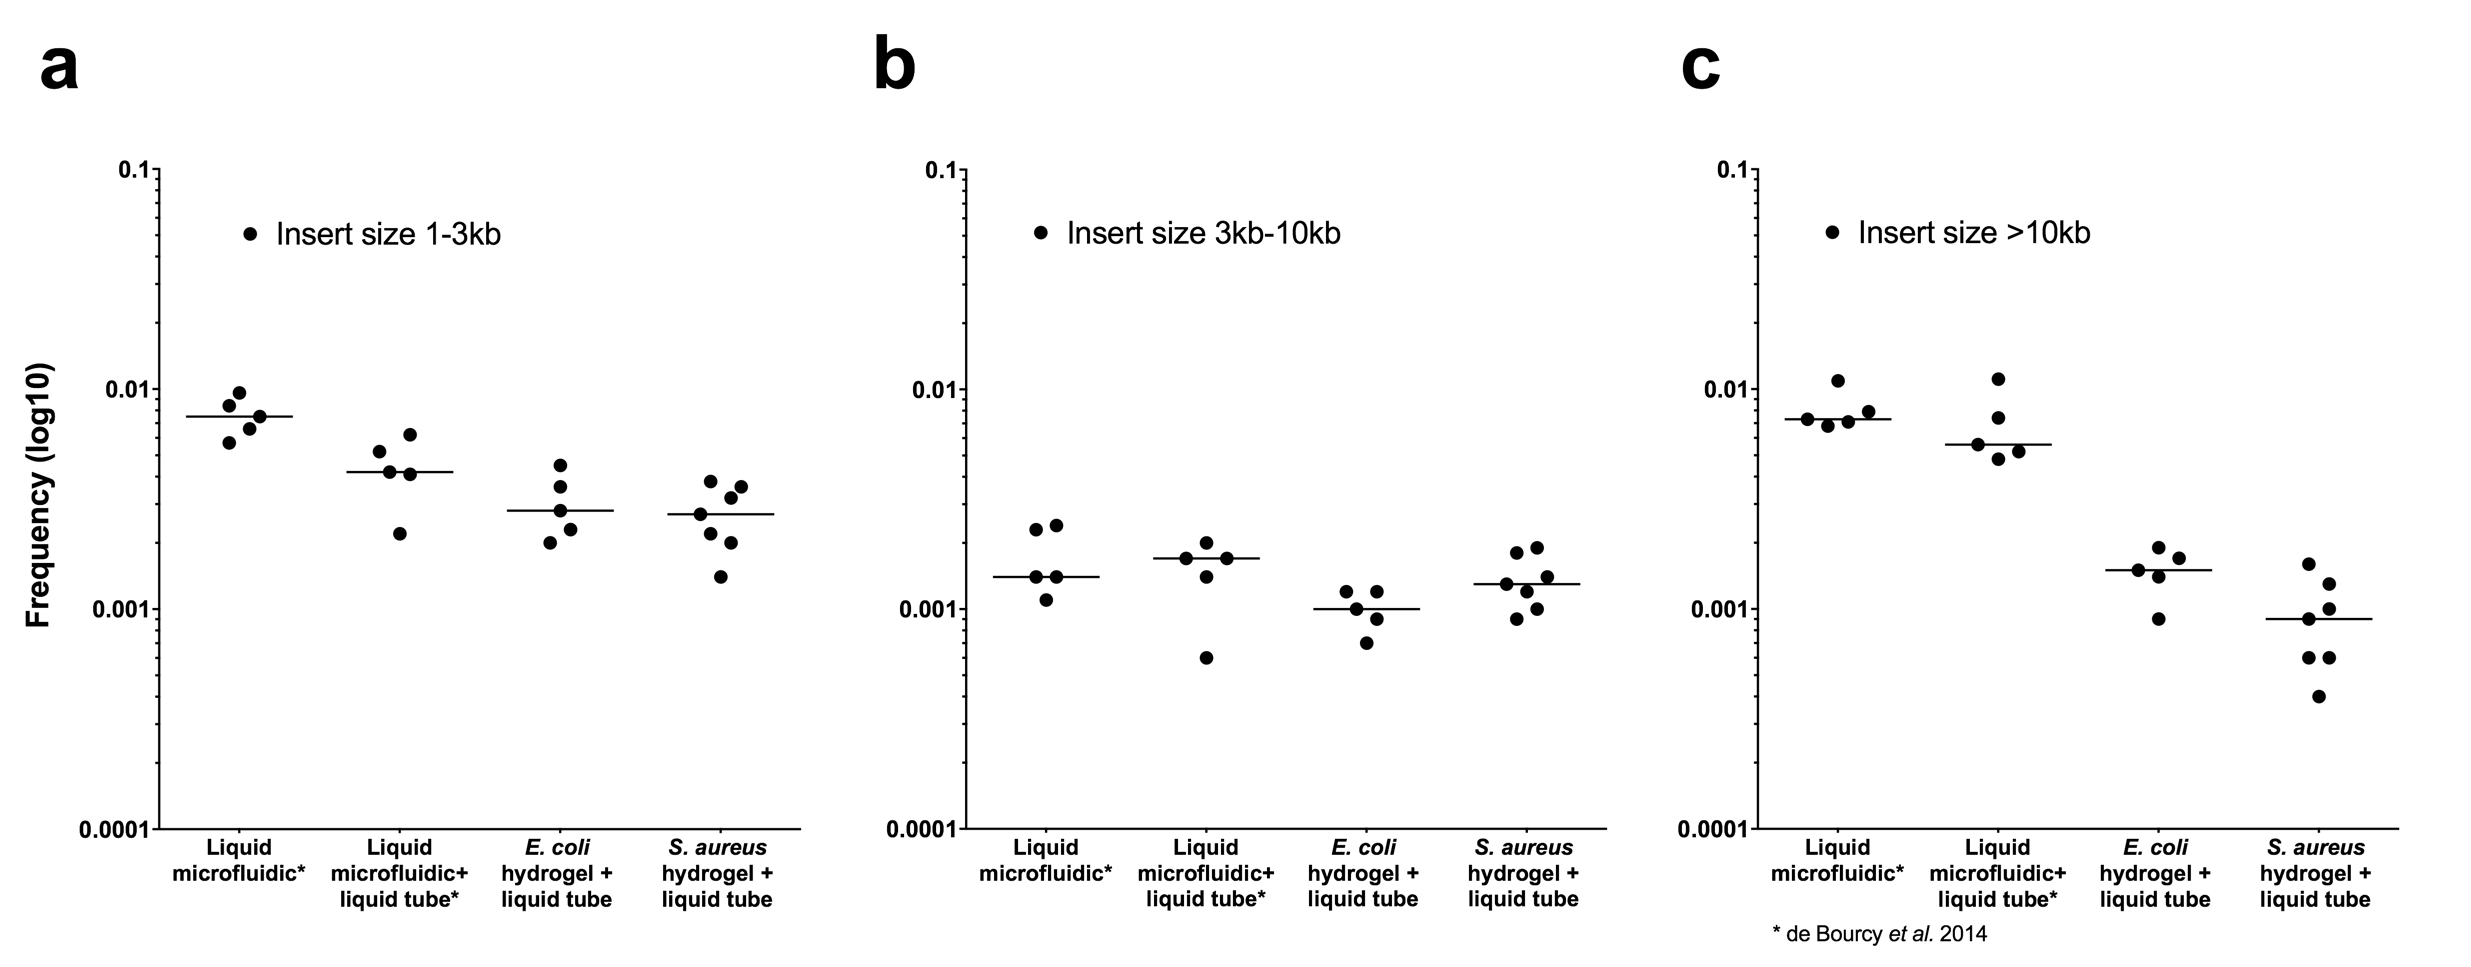
\includegraphics[keepaspectratio,width=\textwidth]{./figures/SuppFig8}
\caption[MDA chimera frequency with different insert sizes, \textit{E. coli} and \textit{S. aureus} data]{MDA chimera frequency with different insert sizes, \textit{E. coli} and \textit{S. aureus} data. a) 1 - 3 kb. b) 3 kb - 10 kb. c) Larger than 10 kb. Centerlines represent the mean value.}
\label{fig:Chimera10k}
\end{figure}

We then analyzed the occurrence of chimeric reads, which are known to occur with high frequency in MDA by a cross-priming mechanism \cite{Lasken:2007db}. Chimeric reads directly confound \textit{de novo} assembly, analysis of rearrangements, and mapped read counting. Our single-cell datasets contained about 0.5\% chimeric reads, approximately five-fold lower than previously published short-read datasets produced using liquid single-cell MDA samples (Fig. \ref{fig:ESMDA}e and Table \ref{tab:MapStatES}). The occurrence of chimeric reads spanning more than 10 kb of the template is even lower (about 0.1\%, Fig. \ref{fig:Chimera10k}), raising the possibility of extracting long-range information from single-cell MDA samples using long-read sequencing. This dramatic reduction in the occurrence of chimeric reads can be understood by restricted diffusion of the MDA intermediates that prevents cross-priming by isolating each portion of the product mixture. It may be the case that substantially all of the chimeras we observed in the punch samples were generated during the liquid-phase secondary amplification reactions. Based on these results, it is likely beneficial to run MDA in PEG hydrogels for all applications at all scales. 

\subsection{In-gel single-microbe MDA - human gut microbiome samples}
Next, we tested the potential of \textit{virtual microfluidics} for single-cell genome sequencing using samples from the Fiji Community Microbiome project (FijiCOMP). The FijiCOMP samples contain a vast uncharacterized diversity of microbial species that differ from those found in the microbiome of Western subjects. The procedure for processing these human stool samples was similar to those for lab-cultured \textit{E. coli} and \textit{S. aureus}, with modifications for initial sample processing and lysis (methods).

\begin{figure}
\centering
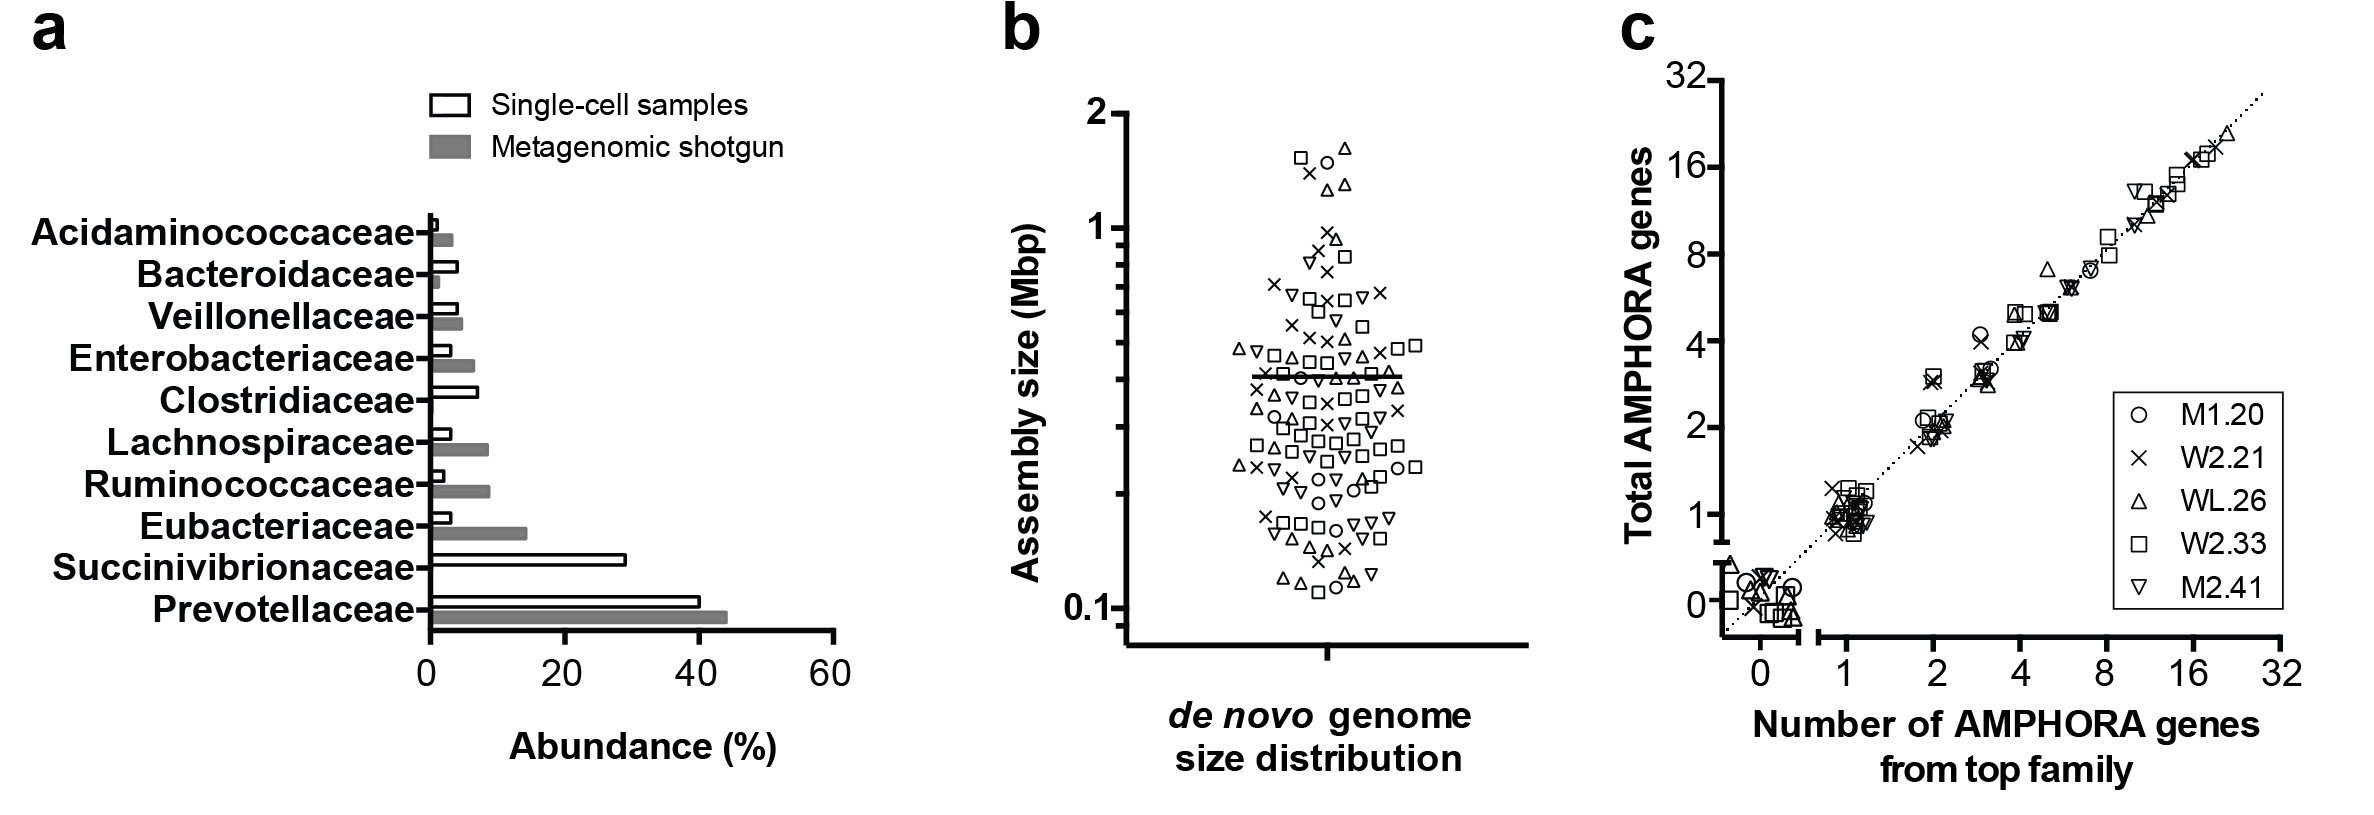
\includegraphics[keepaspectratio,width=1\textwidth]{./figures/Thesis-23.png}
\caption[Fiji microbiome project single-cell whole-genome sequencing.]{Fiji microbiome project (FijiCOMP) single-cell whole-genome sequencing. Here are the results for 117 single-cell data sets from five donor individuals. (a) Distribution of top ten microbial families from single-cell assemblies and metagenome shotgun sequencing. Samples were weighted according to the number of single cells analyzed (Table \ref{tab:MetagenomicFiji}). (b) \textit{De novo} assemblies from single-cell sequencing data ranged from 100 kbp to 2 Mbp. The line indicates the mean assembly size. (c) The total number of AMPHORA genes is nearly equal (dotted line) to the number of AMPHORA genes from the top phylogenetic family for each sample, supporting the assertion that each data set arises from an individual bacterial cell. A Gaussian-distributed random jitter ($\mu$ = 0, $\sigma^{2}$ = 0.1) was applied to enhance visualization.}
\label{fig:Amphora}
\end{figure}

\begin{table}[h]
\centering 
\caption{Overview of 117 FijiCOMP single-cell hydrogel samples}
\label{tab:Fiji117cells}
\begin{adjustbox}{max width=\textwidth}
\begin{tabular}{c|c}
\hline 
Sample categorizations & Number of punches \\
\hline\hline
Low read counts; no assembly & 16 \\
Laboratory contamination (\textit{E. coli}, \textit{P. aeruginosa}) & 29 \\
Human cell sequences amplified & 3 \\
No phylogenetic markers & 80 \\
Enrichment of multiple taxonomies from assemblies & 108 \\
Assembly < 100 kb & 68 \\
\hline
\cellcolor{lightgray}Single-cell assemblies & \cellcolor{lightgray}117 \\
\hline
Total sequenced & 421 \\ \hline
\end{tabular}
\end{adjustbox}
\end{table}

We processed a total of 421 hydrogel punch samples and compared the distribution of organisms detected in our hydrogel samples with the distribution observed from shotgun metagenomic profiling, which showed that the same top microbial families were observed using both approaches (Fig. \ref{fig:Amphora}a and Table \ref{tab:MetagenomicFiji} in methods). Interestingly, the second most abundant microbial family found in the single-cell dataset, the Succinivibrionaceae, was not initially detected but was later confirmed in the shotgun metagenomic data due to its rare representation in the established database using standard methods for the taxonomic assignment such as MetaPhlAn \cite{Segata:2012ts}. This discrepancy highlights the importance of unbiased approaches like single-cell analysis for organisms that are less well represented in reference databases.

We carried out \textit{de novo} assembly of the single-cell datasets and assigned taxonomy to ribosomal gene sequences and 31 \say{single copy} bacterial marker genes at the family level \cite{Wu:2012dh}. This analysis enabled us to make crude assessments of sample purity in the FijiCOMP single-cell datasets (for which we lack strain-specific bona fide reference sequence). Of the 293 assemblies (up to 12 Mbp), we classified 117 as single amplified genomes with assembly size greater than 100 kb and strong enrichment of sequences from a single taxonomy (see Fig. \ref{fig:Amphora} and Table \ref{tab:Fiji117cells}) for the fate of all samples. The purity of single amplified genomes are evaluated with the identity of AMPHORA (AutoMated PhylogenOmic infeRence Analysis) marker genes. AMPHORA genes are a collection of protein-coding marker genes that are single-copy in the genome, universally distributed, and are relatively recalcitrant to horizontal gene transfers \cite{Wu:2012dh}. We identify the number of AMPHORA marker genes and their phylogenines in each single amplified genome. If the total number of AMPHORA genes is nearly equal to the number of AMPHORA genes from the top phylogenetic family, it indicates the dataset arises from an individual bacterial cell (Fig. \ref{fig:Amphora}c). Overall, the data quality observed from these human microbiome bacteria was consistent with the results of our studies with lab-cultured Gram-negative and Gram-positive samples and demonstrates the applicability of the hydrogel method to real-world samples, including lysis and amplification of a variety of naturally occurring microbes.

% In order to test our hypothesis that mobile genes are distributed without geography barrier and interpersonal and intraperson distance. We conducted mobile gene transfer analysis on 117 single-cell datasets. The species information is obtained from with RNAMMER on available 16S or 5S sequence. For cells that lack a 16S sequence, the species is defined by AMPHORA call and the 16S sequence was obtained through RDP. All available 16S sequences was concatenated and the phylogeny distance matrix between all pairs of 16S sequences were calculated using USEARCH \cite{Edgar:2010cv}. The goal was to find distantly related genomes (less than 97\% 16S rRNA similarity). HGT is the best explanation for these because the highly conserved 16S gene evolves about 25-fold more slowly than protein-coding synonymous sites \cite{Smillie:2011jc,Ochman:1999to}. Vertically inherited orthologues should be nearly saturated with wobble basepair mutations in such divergent genomes. After identifying the single cells that are more than 3\% distant, we identified protein-encoding genes for each selected single cells using RAST \cite{Aziz:2008ku}. Each cell's genes were pairwise matched using USEARCH to look for genes that are 100\% identical. We categorize these genes as horizontally transferred genes (HTG). Next, the HTG set is mapped to the database to identify antibiotic resistant genes, virulence factors(VF), insertion sequences and phages. We expect the percent of HGT pairs (pairs of genomes that have more than one 100\% identical genes) to decrease as 16S distance increases from 3\% to 30\%. We also want to find out the difference in numbers and distributions of antibiotic resistant and VF HGTs between different persons and within the same person. In addition, among the shared genes across all Prevotellaces family, we made a phylogeny tree to show the divergence of genes.

\subsection{Random Dispersion Model}
Based on qPCR analysis of the 80 punches, the expected number of punches that have both \textit{E. coli}  and \textit{S. aureus}  is: 

\begin{aligned}
	&P_{\textit{E.coli}} = \frac{14}{80} = 0.175 ; \ \ \ \ P_{\textit{S.aureus}} = \frac{43}{80} = 0.538 \\
	&P_{negative} = \frac{30}{80} = 0.375; \ \ < N_{both  \textit{E.coli} and  \textit{S.aureus}} > = \frac{14}
{80} \times \frac{43}{80} \times 80 = 7.52\\

\end{aligned}

This result is in line with our qPCR result of seven double positive punches (Table \ref{tab:QpcrHydrogel}), indicating the likelihood that the distributions of \textit{E. coli}  and \textit{S. aureus}  across the punch samples are independent as we expected. Furthermore, if we assume a random (Poisson) distribution of microbes in the hydrogel: 

\begin{aligned}
	&P_{\textit{E.coli}}\ (0, \lambda_E) = e^{- \lambda_E} = \frac{66}{80} = 0.825 , \ \lambda_E = 0.192 \\
	&P_{\textit{E.coli}}\ (1, \lambda_E) = \lambda_E \ e^{- \lambda_E} = 0.158 \\
	&P_{\textit{E.coli}}\ (2, \lambda_E) = \frac{\lambda_E^2 \ e^{- \lambda_E}}{2} = 0.01 \\
	&P_{\textit{E.coli}}\ (Single\ cell) = \frac{0.158}{1-0.825} = 90.3\% \\
	&P_{\textit{S.aureus}}\ (0, \lambda_S) = e^{- \lambda_S} = \frac{37}{80} = 0.462 , \ \lambda_S = 0.772 \\
	&P_{\textit{S.aureus}}\ (1, \lambda_S) = \lambda_S \ e^{- \lambda_S} = 0.356 \\
	&P_{\textit{S.aureus}}\ (2, \lambda_S) = \frac{\lambda_S^2 \ e^{- \lambda_S}}{2} = 0.138 \\
	&P_{\textit{S.aureus}}\ (Single\ cell) = \frac{0.356}{1-0.462} = 66.2\% \\

\end{aligned}

The low probability value for the occurrence of single \textit{S. aureus} is calculated based on the high number of hydrogel punches that were identified as \textit{S. aureus} by qPCR. To bring down the value, a more dilute sample of \textit{S. aureus} should be used (Table \ref{tab:RandomDispersion}). 

\begin{table}[h]
\centering 
\caption{Microbe occurrence probability}
\label{tab:RandomDispersion}
\begin{adjustbox}{max width=0.8\textwidth}
\begin{tabular}{c||ccc}
\hline 
 & P_{\textit{E.coli}}(0)=0.825 & P_{\textit{E.coli}}(1)=0.158 & P_{\textit{E.coli}}(2)=0.01 \\
\hline\hline
P_{\textit{S.aureus}}(0)=0.463 & 0.38 & 0.073 & 0.0046 \\
P_{\textit{S.aureus}}(1)=0.356 & 0.29 & 0.056 & 0.0036 \\
P_{\textit{S.aureus}}(2)=0.138 & 0.114 & 0.022 & 0.0014 \\
\hline
\end{tabular}
\end{adjustbox}
\end{table}

\section{Conclusion}
\textit{Virtual microfluidics} enables high throughput whole genome amplification and serial reagent exchange in an easy-to-use, benchtop format that requires no special equipment or environmental control. Here we show preparative amplification and recovery of single bacterial genomes for \textit{ex-situ} analysis of lab-cultured control cells and the human gut microbiome by next-generation sequencing (NGS).

\textit{Virtual microfluidics} establishes a new paradigm in single-molecule and single-cell analysis with dramatically different characteristics than established microfluidic approaches. Besides reducing the production of chimeras in MDA, the unique physical characteristics of the engineered hydrogel environment may provide a means for enhancing coverage extent and uniformity from WGA and WTA samples through the self-limiting reactivity within each virtual compartment, similar to a recently reported emulsion approach \cite{Fu:2015gl}. In addition, the straightforward addition and removal of reagents to/from product clusters \textit{en masse} and excellent optical access ideally suit the \textit{virtual microfluidics} system for rare-cell assays incorporating \textit{in situ} labeling of cells or product clusters. We expect that \textit{virtual microfluidics} will find application as a high-throughput platform for single-cell sample preparation.

% Talk about environmental microbiome field work 

\section{Materials and Methods}
\subsection{In-gel single-microbe MDA - \textit{E. coli}  and \textit{S. aureus} }
Antibiotic resistant \textit{Staphylococcus aureus subsp. aureus} (GFP) NCTC 8325 and \textit{Escherichia coli} (RFP) BL21 strains were obtained as cryogenic stocks. For each culture, the frozen stock was inoculated in 5 mL LB broth and cultured at 37 $^{\circ}$C overnight. 10 $\mu$L of 25 mg\slash mL Chloramphenicol was added to \textit{S. aureus}  culture and 5 $\mu$L of 50 mg\slash mL Ampicillin was added to the \textit{E. coli}  culture. 50 $\mu$L and 20 $\mu$L of each overnight culture were added to fresh 5 mL LB broth with the respective antibiotic concentration. After two hours incubation (to achieve exponential growth phase), 1 mL of each culture (O.D. 600 nm = 0.2) was centrifuged for 2 min at $>$10 krpm and the pellet was washed with 500 $\mu$L PBST (1\% Tween--20) twice. The equal ratio mixture of microbes were diluted to 206,000 cells\slash mL and 1 $\mu$L of each was encapsulated in the same hydrogel sample to produce an average of less than 1 microbe per 500 $\mu$m diameter view. In addition to the hydrogel MDA reaction mix described above, lysozyme (Sigma, final concentration 2.5 mg\slash mL) and lysostaphin (Sigma, final concentration 0.1 mg\slash mL) were added to the mix. The hydrogel was left at RT to let crosslink for 20 minutes and cross-linked hydrogels were incubated at 37 $^{\circ}$C for 1 hour for microbe lysis and heated to 95 $^{\circ}$C for 5 min to denature genomic DNA before rapid quenching on ice. 1 $\mu$L of REPLI-g sc Polymerase (Qiagen) diluted in 2 $\mu$L water was then added on top of the hydrogel and allowed to diffuse into the gel. Next, the gel chamber is resealed and MDA was conducted for 10 hours. After the MDA reaction, the sample was heated to 65 $^{\circ}$C for 5 min to deactivate phi29 polymerase.

\subsection{Image acquisition and analysis}
Z stack images were taken by a Nikon ultra-fast laser scanning confocal microscope with the pinhole = 1.2, HV = 112, offset = 0, laser wavelength = 561 nm, laser power = 1.3 to 1.5, using a 20$\times$ objective on Galvano mode. The acquisition speed was 1 frame\slash sec and z step size was 0.95 $\mu$m. On the inverted microscope, z stack images were taken with the exposure time 100 ms, Lumencor excitation power 10\%, binning size 2 and z step size 10 $\mu$m. Both z Stacks were first processed into max intensity projections in FIJI. Max projection tif files were then loaded into MATLAB. Background was obtained by applying a Gaussian filter of hsize 200 and sigma 50. All max projections were background-subtracted and thresholded at 2 $\sim$ 2.5$\times$ standard deviations above the mean intensity. Cluster count, cluster area (radius), and cluster mean intensity were obtained with the bwconncomp and regionprops functions.

For whole gel (25 $\mu$L, 9mm by 9mm) microbe density approximation, I imaged the gel with a 4$\times$ objective in a 5 $\times$ 5 grid with a 31\% overlap. The 25 images were stitched using the FIJI stitching function. Fluorescent DNA clusters were counted and only gels with the appropriate clusters' range and dispersion (60 $\sim$ 80 per gel) were selected for hydrogel cluster retrieval. Images of the sampled locations were acquired but not used to guide sampling, sample preparation, or data analysis in this case.

\subsection{MDA product cluster retrieval}
In order to identify and retrieve a regular array of punches (not guided by cluster image data), we produced a tape stencil to guide the punch tool (Adhesive Applications High Tack Silicone Film Tape). We laser cut the double-sided tape with a 9 $\times$  9 array of 500 $\mu$m diameter circles that has a center-to-center distance of 947 $\mu$m (Full Spectrum Laser LLC MLE--40). The tape stencil was applied on top of the frame seal plastic cover. The gel was peeled off the glass slide by allowing it to adhere to the plastic cover. The gel is then punched with a 1 mm diameter steel punch (Militek) and the micro-samples collected in a 96 well LoBind twin.tec plate (Eppendorf). The steel punch was cleaned with bleach and 70\% Ethanol after each use.

\subsection{BLAST analysis and read assignment for \textit{E. coli} and \textit{S. aureus}}

\begin{figure}
\centering
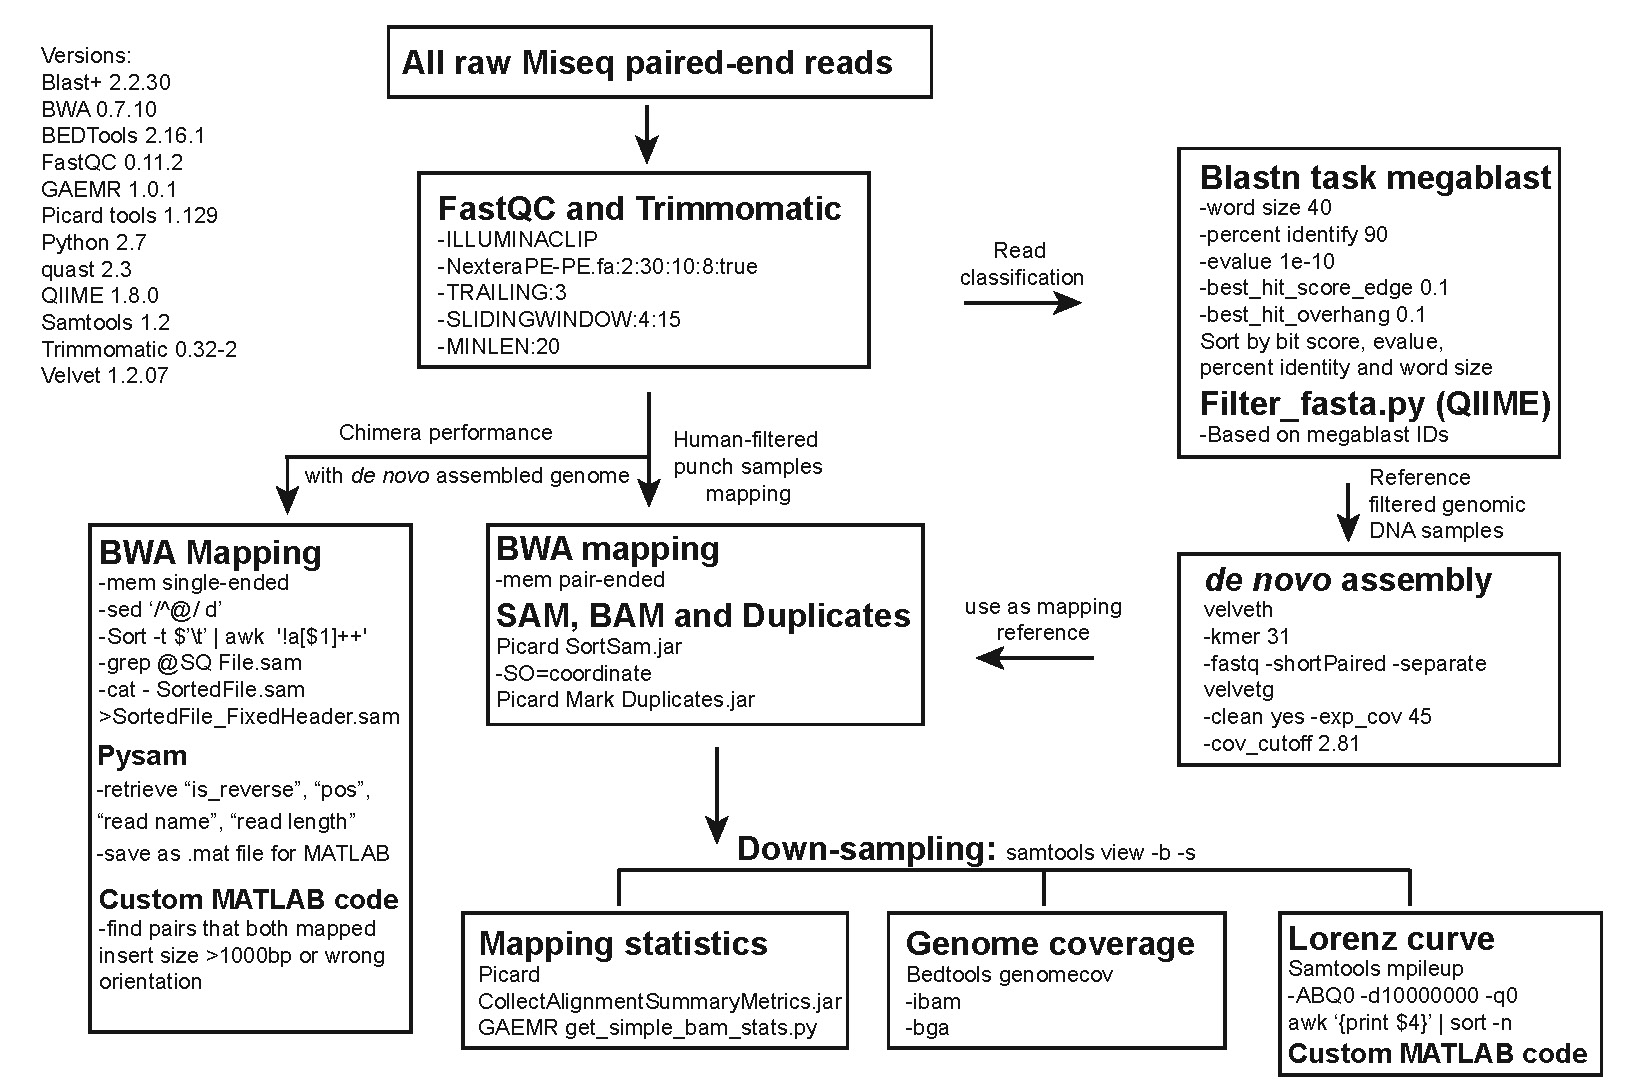
\includegraphics[keepaspectratio,width=1\textwidth]{./figures/SuppFig6.jpg}
\caption[NGS data analysis schematic for \textit{E. coli} and \textit{S. aureus}]{NGS data analysis schematic for \textit{E. coli} and \textit{S. aureus}. The analysis workflow is shown with a combination of bioinformatic tools, python scripts and MATLAB scripts.}
\label{fig:ESDataAnalysis}
\end{figure}

To characterize all samples after quality trimming, each sample (R1 from each read pair) was blasted (task megablast) with the parameters listed in Fig. \ref{fig:ESDataAnalysis}. The BLAST database for \textit{E. coli} consists of three \textit{E. coli} genomes (strain BL21, MG1655 and W3110). The \textit{S. aureus} database consists of the genomes of strain 8325, TW20 and USA300. Univec, Plasmid and Human genome (GRCH38) databases were downloaded from NCBI. All databases were produced using makeblastdb and blastdb\_alias tool. Each read was mapped to all five databases (\textit{E. coli}, \textit{S. aureus}, Univec, Plasmid, and Human db) and the results were ranked based on bit score, e-value and then percent identity. We assigned each read to one of the source databases based on the top hit. Using the filter\_fasta.py tool in QIIME  \cite{Caporaso:2010jf}, we selected reads that did not map to any of the five databases for further analysis. We ran BLAST against the nt database to characterize these reads (Table. \ref{tab:BlastReadsES}). 

\subsection{Secondary liquid MDA and PCR screening - cultured \textit{E. coli} and \textit{S. aureus}}
The retrieved hydrogel punch was dissolved and denatured in 1 $\mu$L of 1 M KOH with 0.1 mM EDTA and 0.1 M DTT at 72 $^{\circ}$C for 10 min before neutralization in 1 $\mu$L stop solution (Qiagen REPLI-g single cell kit. Approximately 0.06 $\mu$L of hydrogel and 10 pg of DNA was captured for a cluster. The neutralized product was added to 12.5 $\mu$L REPLI-g sc reaction mix with 1 $\mu$L of phi29 polymerase. The secondary MDA reaction was incubated for 10 hours before polymerase deactivation at 65 $^{\circ}$C for 5 min. The DNA products from MDA were cleaned by the SPRI procedure in 1.8:1 beads to DNA volume (Beckman Coulter). Each sample was analyzed for the presence of \textit{S. aureus} and \textit{E. coli} marker loci by four sets of primers (Table \ref{tab:ESprimerList}) in standard qPCR reactions with Jumpstart Taq 2$\times$ ready mix (Sigma Aldrich), 1$\times$ Evagreen (Biotium), 1$\times$ ROX (Invitrogen) and 1 $\mu$M primers in Stratagene M3005. Both melting curve analysis and agarose gel electrophoresis (not shown) were used to support the QPCR results.

\begin{table}
\caption{PCR primer sequences}
\label{tab:ESprimerList}
\begin{center}
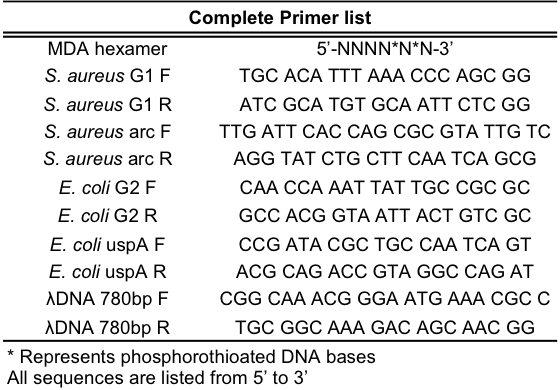
\includegraphics[width=0.5\linewidth]{./figures/ESprimerList}
\end{center}
\end{table}

\subsection{WGS library construction and sequencing}
We quantified the purified MDA products using the Qubit\slash Quant-IT HS assay (Thermo Fisher Scientific) and normalized samples to 5 ng\slash $\mu$L. All SPRI procedures were conducted on the Bravo robotic system (Agilent Technologies). Purified DNA (5 ng) was then added to 1 $\mu$L of 5$\times$ tagmentation DNA buffer, 2 $\mu$L $\text{H}_2\text{O}$ and 1 $\mu$L Nextera Tagmentation DNA enzyme (Illumina). The mixture was first incubated at 58 $^{\circ}$C for 10 min. With the addition of 0.5 $\mu$L of 1\% SDS, it was then incubated at 68 $^{\circ}$C for 10 min, 4 $^{\circ}$C for 3 min and 25 $^{\circ}$C for 3 min to stop the tagmentation reaction. Another SPRI clean-up was carried out, followed by PCR library barcoding using Index primer N7 and S5 (Illumina) with the thermal protocol: 72 $^{\circ}$C for 3 min, 98 $^{\circ}$C for 30 sec, 12 cycles of 98 $^{\circ}$C for 10 sec, 60 $^{\circ}$C for 30 sec, 72 $^{\circ}$C for 30 sec and a 5 min final extension at 72 $^{\circ}$C. Samples were barcoded uniquely in the PCR step using standardized custom sample barcodes (Broad Institute Genomics platform). The PCR products were purified with SPRI twice with 1:1 beads to DNA volume and library quantification was carried out with the Quant-It assay (Thermo Fisher Scientific) and the KAPA library quantification kit (KAPA Biosystems). Library normalization and pooling were conducted on the Janus Mini Varispan workstation (PerkinElmer). For \textit{E. coli} and \textit{S. aureus} samples, an average of 0.7 million paired-end reads were allocated for each sample in a MiSeq 500 cycle v2 run (Illumina). For stool samples, about 1 M reads ($>$ 50$\times$) were allocated to each sample on HiSeq 2500 2$\times$101\slash 125 runs (Illumina). 

\subsection{NGS data analysis for \textit{E. coli} and \textit{S. aureus}}
Data quality was first visualized using FastQC (Babraham Bioinformatics). All data were trimmed using trimmomatic \cite{Bolger:2014ek} and human reads were filtered out with BLAST and QIIME. Each pair of trimmed and filtered reads was piped into BWA and mapped to the custom reference sequences (Fig. \ref{fig:MappingES}). SAMtools view was used to produce BAM files, and Picard tools (Broad Institute) deployed to mark duplicate reads. The data analysis workflow is illustrated in Fig. \ref{fig:ESDataAnalysis}. The samples included two positive-control purified genomic DNA samples, seven hydrogel MDA punches identified as \textit{E. coli} only by qPCR, seven punch samples identified as \textit{S. aureus} only by qPCR, and seven punch samples identified by qPCR as double negative. Mapping statistics were obtained using the GAEMR (Broad Institute) get\_simple\_bam\_stats.py tool (Table \ref{tab:MapStatES}). Genome coverage was obtained using Bedtools genomecov. Lorenz curves were obtained by first processing BAM files (duplicates marked) using samtools mpileup and then ranking the ascending coverage per base pair. Single-cell \textit{E. coli} MDA data from de Bourcy \textit{et al}. 2014 were downloaded from NCBI Sequence Read Archive (SRA) and analyzed by the same procedures. 

\begin{figure}
\centering
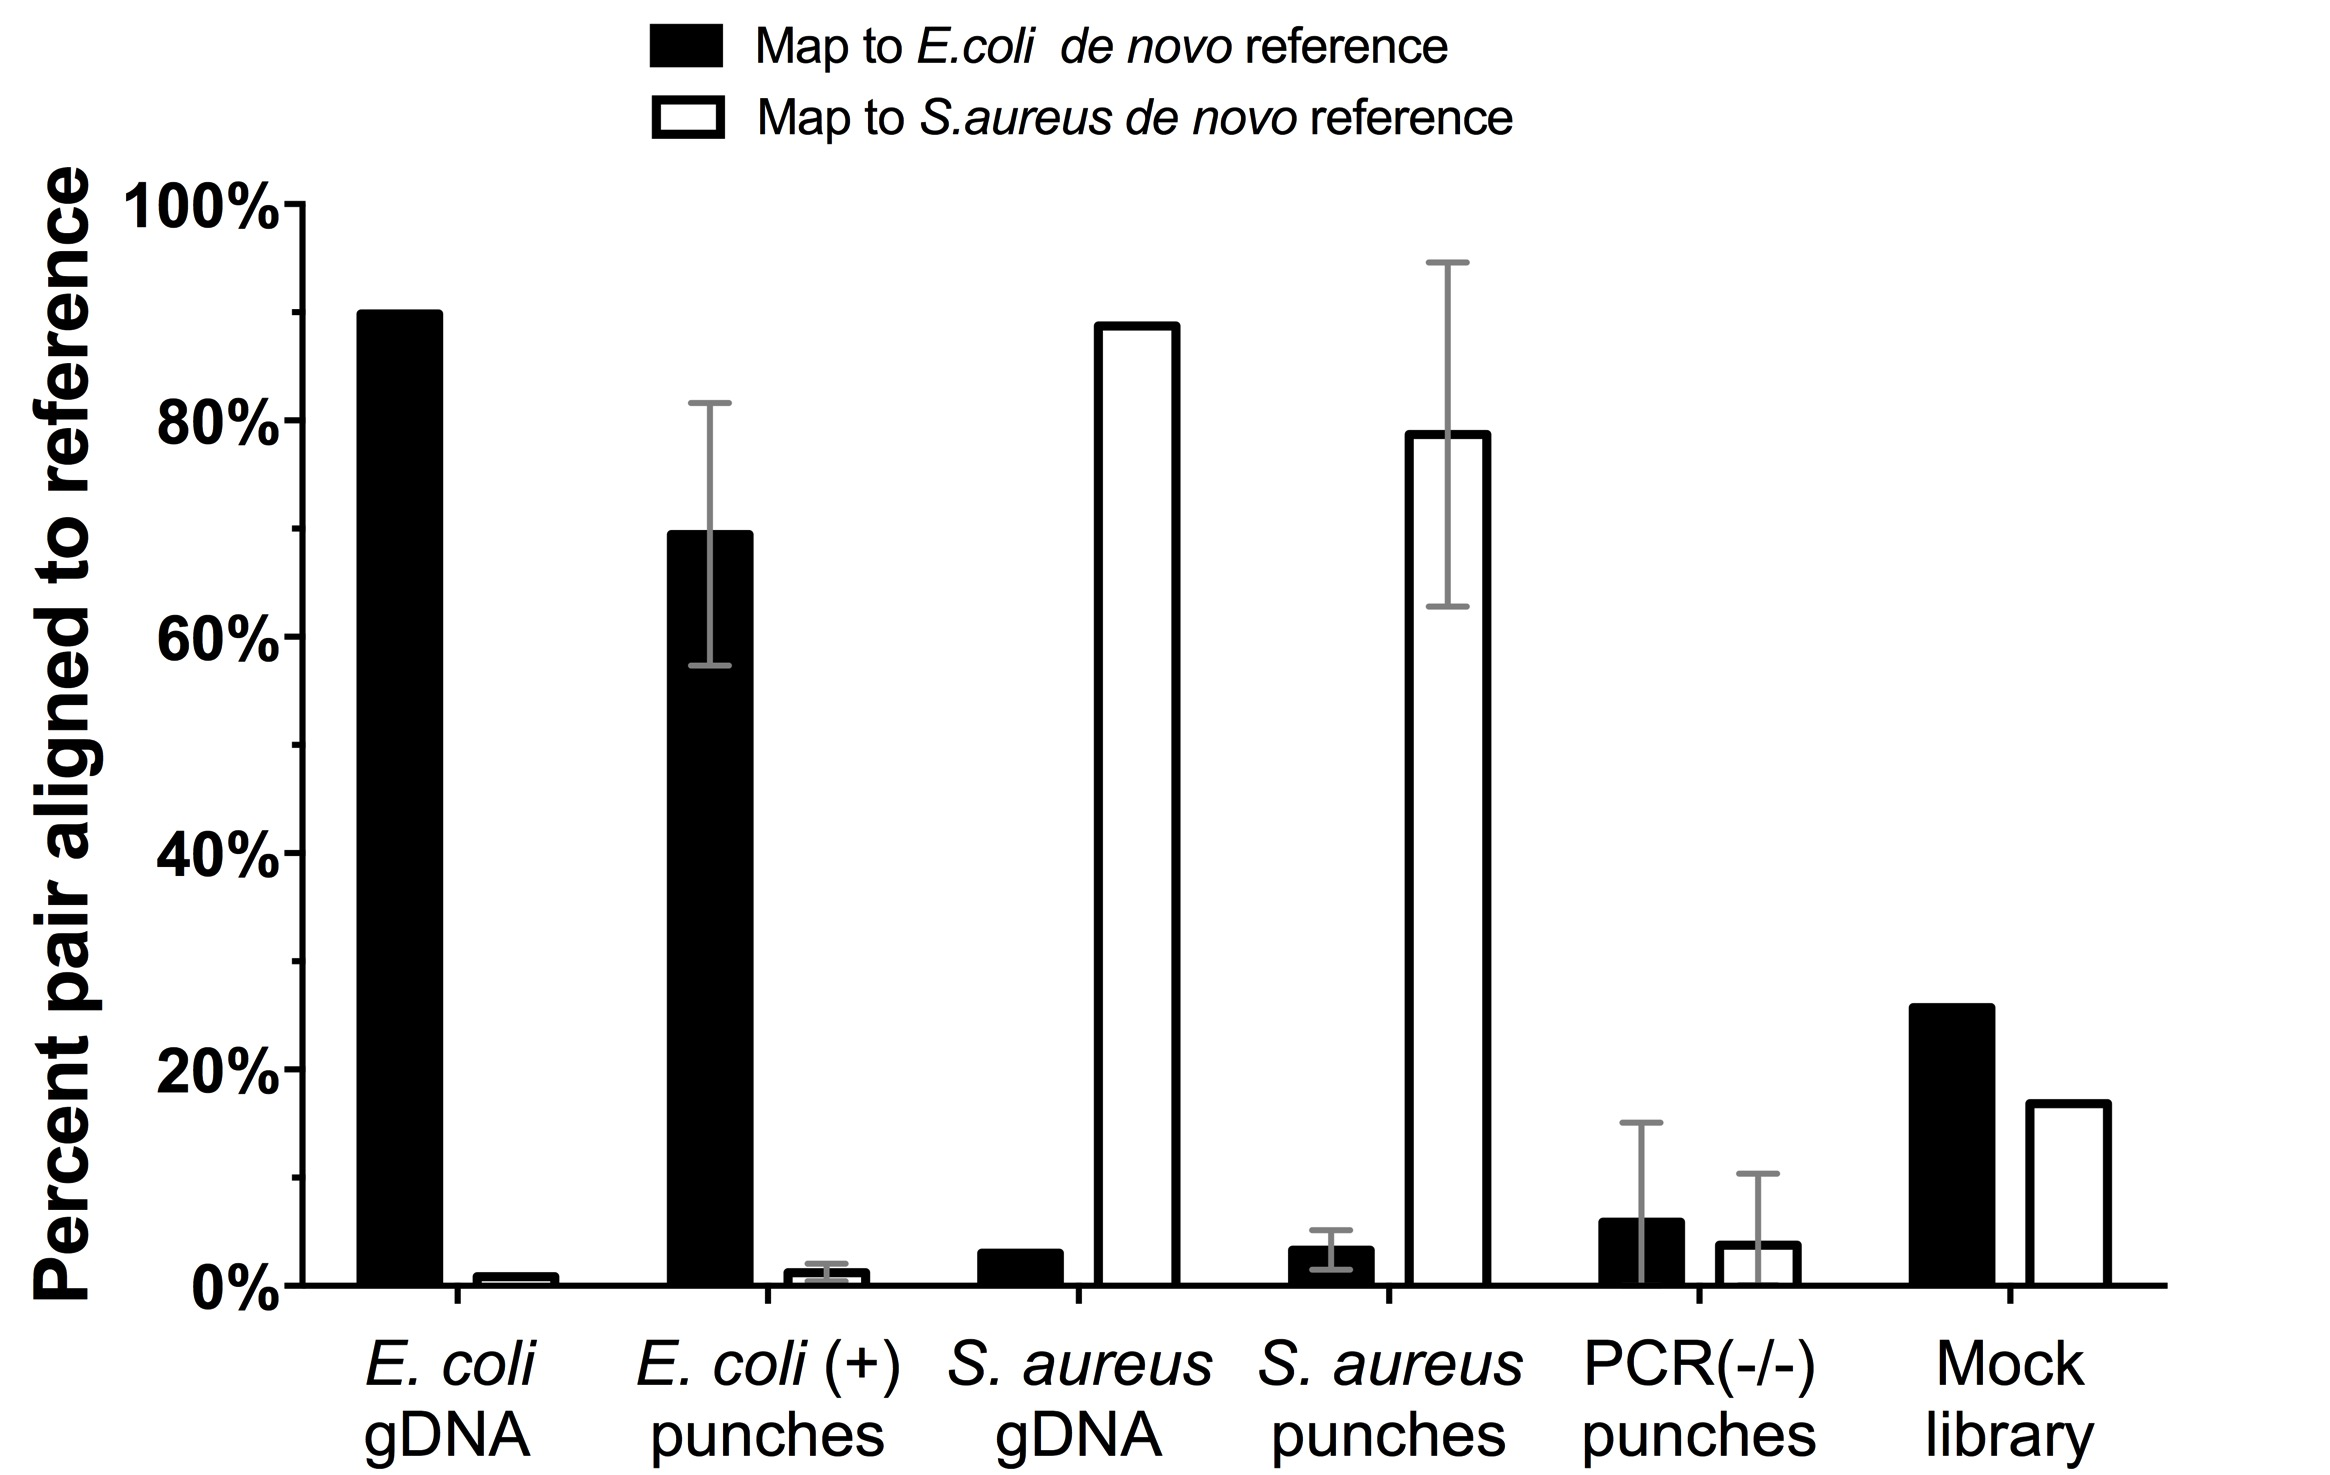
\includegraphics[keepaspectratio,width=0.6\textwidth]{./figures/SuppFig7.jpg}
\caption[Mapping single-cell genomes to references]{Mapping single-cell genomes to references. Single-cell samples were mapped to \textit{E. coli} and \textit{S. aureus} reference sequences with mean percent pair aligned and standard deviation shown. (n = 5 for \textit{E. coli} punches, n = 7 for \textit{S. aureus}, n = 7 for negative punches).}
\label{fig:MappingES}
\end{figure}

\begin{table}
\caption{Mapping statistics, \textit{E. coli} and \textit{S. aureus}}
\label{tab:MapStatES}
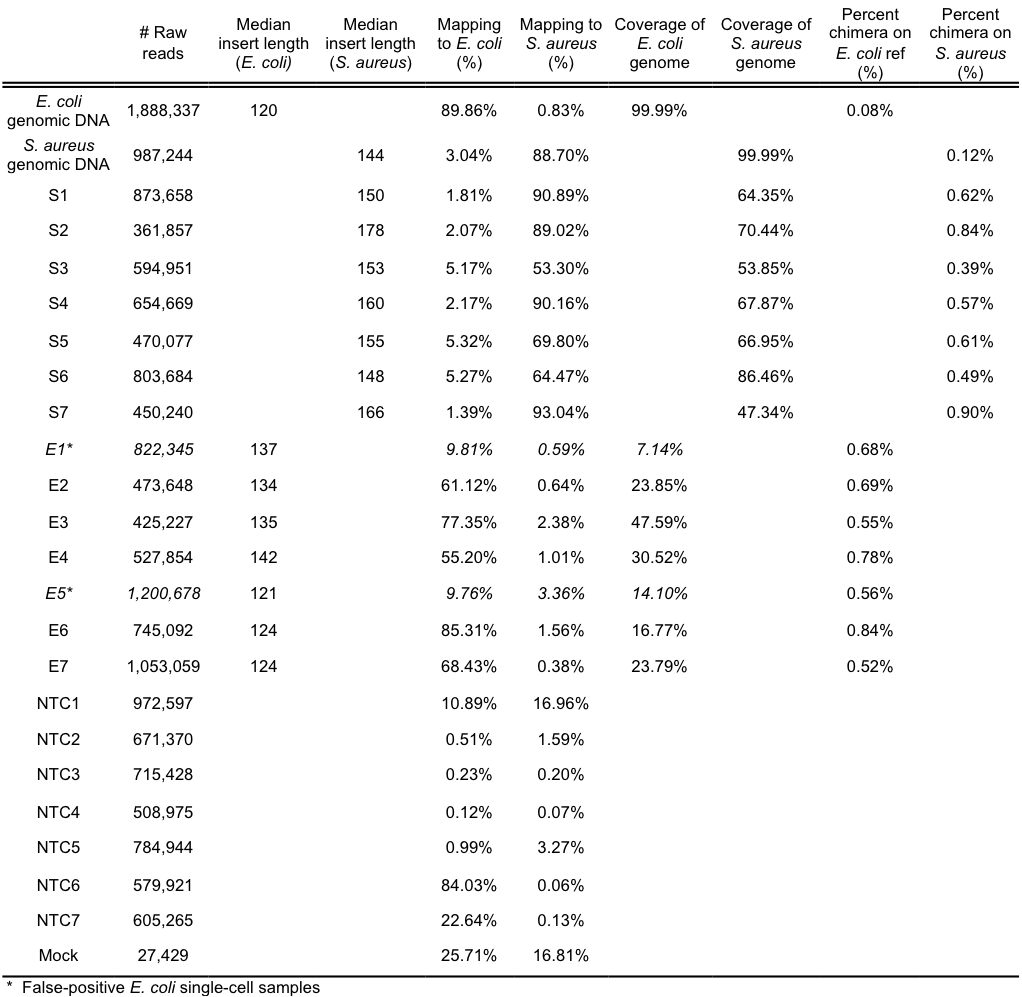
\includegraphics[width=\linewidth]{./figures/MapStatES}
\end{table}

Genome Coverage Completeness Estimation: note that some studies in the field report data from quality-filtered (`cherry-picked') cells, which dramatically improves quality statistics such as average coverage. In this study, we report data on complete sets of single-cell MDA reactions. 

\subsection{Custom reference generation by de novo assembly for \textit{E. coli} and \textit{S. aureus}}
The gDNA \textit{E. coli} (BL21) and \textit{S. aureus} (8325) positive-control data were assembled and curated to create custom reference genome sequences. Raw sequencing files were quality trimmed using Trimmomatic (Fig. \ref{fig:ESDataAnalysis}). We blasted the trimmed files against respective reference databases and filtered described previously with the parameters listed in in Fig. \ref{fig:ESDataAnalysis}. Hit reads were filtered out of the sequencing files using the QIIME filter\_fasta.py tool. The filtered and trimmed files were assembled into unordered contigs with velvet. We mapped (BWA) unordered contigs to their closest NCBI reference genome (NC\_012971 and NC\_007795.1 respectively). The resulting SAM files were ranked on mapped length in descending order. Using a custom MATLAB function, we created a reference genome backbone consisting of only `-' with the same size as the reference genome and wrote sequences on it with only the top SAM mapping sequence for each contig. We conducted the same assembly process for the genomic DNA (\textit{E. coli} DH10B) data from de Bourcy \textit{et al.} 2014 using reference genome NC\_010473.1. Assembly statistics are listed in Table \ref{tab:deNovoAssemblyES}. Custom MATLAB function, python codes and shell scripts are included in the supplementary software zip file in Xu \textit{et al.} 2016. 

\begin{table}
\caption{\textit{de novo} assembly statistics, \textit{E. coli} and \textit{S. aureus}}
\label{tab:deNovoAssemblyES}
\begin{center}
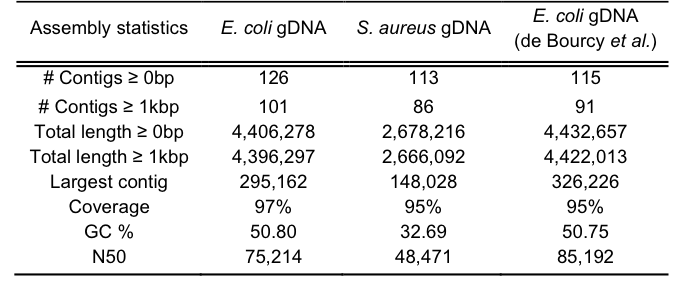
\includegraphics[width=0.7\linewidth]{./figures/deNovoAssemblyES}
\end{center}
\end{table}

Random subsampling of mapped reads for \textit{E. coli} and \textit{S. aureus}
Duplicates-marked BAM files were down-sampled using samtools and bootstrapped with random number seed 0 to 9 for each depth. See Table \ref{tab:DownsamplingESD} for more information. 

\begin{table}
\caption{Downsampling on mapped reads from single-cell MDA samples}
\label{tab:DownsamplingESD}
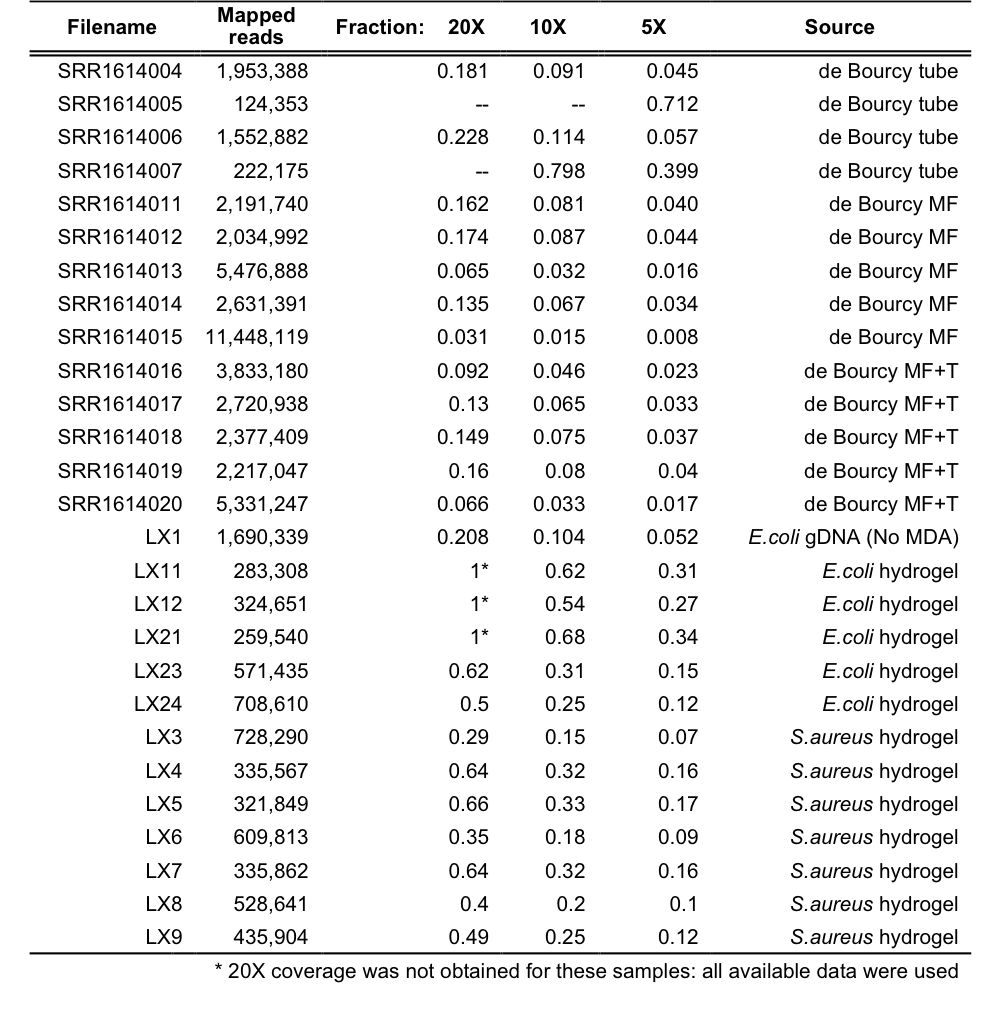
\includegraphics[width=\linewidth]{./figures/DownsamplingESdeBourcy}
\end{table}

% Need to rework 
\subsection{Chimera statistics for \textit{E. coli} and \textit{S. aureus}}
To make the chimera statistics comparable, we used \textit{de novo} assembled genome sequences (described below) from bulk genomic DNA samples as the reference. We mapped read 1 and read 2 from each sample single-ended using BWA. We sorted the SAM file by read index. We used a custom python code to import pysam in order to pair up the `read index', `mapping position', `is-reverse', and `read length' information into a .mat file. With a customized MATLAB script, we calculated the insert size for each read pair and checked their relative orientation. We filtered out pairs that were mapped one-ended. The chimera percentage was calculated as the (number of properly orientated read pairs with insert size more than 1000 bp + number of read pairs of wrong orientation)\slash Total number of read pairs.

\subsection{In-gel single-microbe MDA - human gut microbiome samples}
We received ethics approvals for human subjects research from the Columbia University IRB, Massachusetts Institute IRB, Broad Institute IRB, and two research ethics committees in Fiji: HRERC at CMNHS, FNU and FNHRERC at MoHFiji Ministry of Health. The Fiji Community Microbiome Project (FijiCOMP) study participants from 5 agrarian villages within the Fiji Islands. This project provided stool samples stored in 20\% glycerol within 30 minutes of voiding and were frozen at --80 $^{\circ}$C. Five participants were analyzed for single-cell studies: M1.20, W2.21, WL.26, W2.33, M2.41 (Table \ref{tab:MetagenomicFiji}). 10 $\mu$L of thawed cells were resuspended in 500 $\mu$L PBST (0.1\%). Samples were sonicated for 20 seconds and filtered through 35 $\mu$m Nylon mesh and 5 $\mu$m membrane (Pall Corp.) to collect filtrate with a 500 $\mu$L PBST wash. Samples were further diluted 1 to 500 $\sim$ 1 to 2000 fold in PBST to reach the final concentration of $\sim$ 30 cells\slash $\mu$L. The diluted cell samples (2 $\mu$l) then underwent alkaline lysis (1.5 $\mu$L D2 buffer) for 15 minutes at room temperature, after which the solution was neutralized (1.5 $\mu$L Stop solution). Hydrogel monomer mix (1.3 mg 4-Arm PEG Acrylate and 0.9 mg SH-PEG-SH) and MDA master mix were gently pipetted down the wall of each sample tube. MDA master mix includes 1$\times$ phi 29 buffer (NEB), 50 $\mu$M random hexamers with two phosphorothioate bonds at 3' terminus, 2.5\% DMSO, 0.4 mM dNTP, 0.5 mg\slash mL BSA, 500 nM SYTOX Orange (Invitrogen) and 1 $\mu$L REPLI-g SC Polymerase (Qiagen). Only gentle tapping was used to ensure reagent mixing, in order not to disrupt the lysed microbes and denatured genomes. 25 $\mu$L of each microbial suspension was added into a frame-seal chamber, the sealed chamber was incubated at 30 $^{\circ}$C for 12 hours, followed by 65 $^{\circ}$C for 5 mins.

\begin{table}
\caption{Metagenomic shotgun profiling weighted with single-cell samples}
\label{tab:MetagenomicFiji}
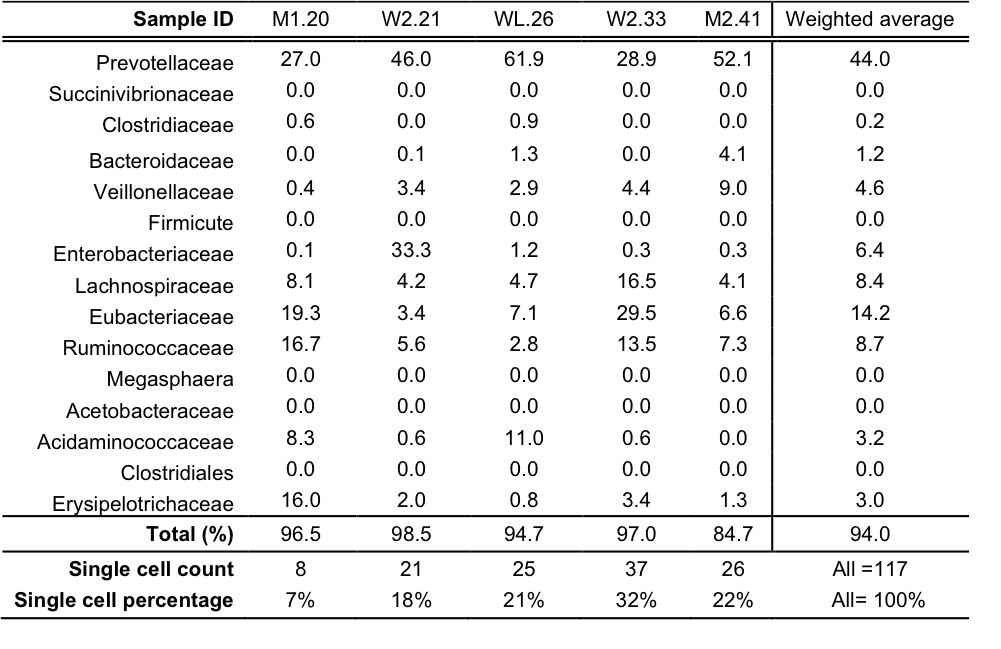
\includegraphics[width=\linewidth]{./figures/MetagenomicShotgunProfilingFiji}
\end{table}

\paragraph{Secondary In-gel MDA - human gut microbiome samples}
Hydrogel punches (approximately 0.24 $\mu$L of hydrogel and 10 pg of DNA if a cluster was captured) were dissolved and denatured in 1 $\mu$L of 400 mM KOH with 0.1 mM EDTA and 0.1 M DTT at 72 $^{\circ}$C for 10 min before neutralization in 1 $\mu$L stop solution (Qiagen REPLI-g single cell kit). The neutralized product was added to 8 $\mu$L hydrogel and MDA master mix to reach a final volume of 10 $\mu$L for second round MDA reaction in hydrogel. The MDA reaction was incubated for 10 hours at 30 $^{\circ}$C before polymerase deactivation at 65 $^{\circ}$C for 5 min. The 10 $\mu$L gel was dissolved with 10 $\mu$L 400 mM KOH for 5 mins at 72 $^{\circ}$C, and then neutralized with 6.6 $\mu$L 2.5\% acetic acid.

\paragraph{Pre-processing and assembly of single-cell genomes from stool}
First, we removed the adapter sequences from single-cell libraries using TRIMMOMATIC \cite{Bolger:2014ek} (TRAILING:3 MINLEN:40). To ensure that human DNA was not captured in our single-cell libraries, we screened single-cell amplicons against the human genome (GRCh38 reference) using BMTagger \cite{Rotmistrovsky:CVigB6Il} (default). We screened our amplicons against \textit{E. coli} references (BL21 and DH10B) using BMTagger. Overall, the level of contamination was small (around 0.01\%). We also screened against \textit{Pseudomonas} (PAO1) and \textit{Staphylococcus} (NCTC 8325) genomes, which were sequenced alongside our libraries, to ensure no chimeric reads formed during sample preparation with contaminating sequences from other cultures in our lab that confounded our analyses. Finally, single genome amplicons were quality filtered (Phred score > 3), and filtered for reads that were less than 45 bp. Amplicons were then assembled using SPAdes (v3.6.0) (--careful) \cite{Bankevich:2012ih}. We retained genomes where at least 100 kb could be assembled.

\paragraph{Assessing the fidelity of single-cell genomes from stool}
To further vet the quality and purity of our assemblies, we used BLAST to assign taxonomies to a set of 31 predetermined core genes that are both phylogenetically conserved and single copy in almost all genomes \cite{Wu:2012dh}. Although we could not identify the full set of 31 core genes in any of the assemblies, we were able to easily distinguish cases where two or more cells were sequenced together from those in which there was a single cell. Additional validation of the single-cell assemblies included quantifying the levels of contamination using CheckM \cite{Parks:2015hs} and examining the number and taxonomy identified using RNAmmer \cite{Lagesen:2007ud}. CheckM accesses the quality of a genome using a broader set of marker genes specific to its inferred lineage within a reference genome tree and provides estimates of genome completeness and contamination percentages. RNAmmer uses hidden Markov models trained from ribosomal RNA databases to predict the rRNA species. The extent and contiguity of our assemblies was documented by reporting assembled genome size, N50, the number of contigs, CheckM completeness percentage, CheckM contamination percentage and notes on RNAmmer classification in an Excel file in Xu \textit{et al.} 2016.

Notably, some microbes can be difficult to isolate from human stool samples due to the cells' tendency to break or aggregate. Some of the punch samples with low numbers of AMPHORA genes could be the result of broken cells containing reduced genomic representation or free genomic DNA fragments, while samples with evidence for multiple taxonomies could have resulted from cell aggregates. Stool samples are also fairly complex and contain a lot of particulate matter that complicates sample processing. In principle, genes from samples with sequences of variable taxonomy could arise for several reasons: the products of multiple cells being collected in a single punch, downstream contamination in the second round MDA or library construction steps, informatic demultiplexing, or from taxonomic mis-classification of hard-to-assign sequences.

\paragraph{Analysis of metagenomic shotgun reads from stool}
FijiCOMP metagenomic samples, each containing roughly 50 million paired-reads, were profiled using MetaPhlAn \cite{Segata:2012ts}. Metagenomic samples were also aligned to the SILVA rRNA database (v.115) to determine the presence of organisms from the Succinivibrionaceae family. Based on alignments to the SILVA rRNA database, we find that organisms within the Succinivibrionaceae family are in fact highly abundant in the FijiCOMP metagenomic data, with average FPKM (Fragments Per Kilobase of transcript per Million mapped reads) values around 26,000.


% From Brito et al.
% ``However, despitethe high prevalence of genes and broader gene functions, we found that 34.9\% of the gene contexts, defined as the set of unique combinations between adjacent genes that were observed, were specific to individuals; very few of these gene contexts were conserved across populations''
% ``Together, high recombination rates and population-specificity support the notion that environmental selection on individual genes, rather than dispersal limitation alone, plays a key role in driving gene abundances.''
% ``Second, even though each of the mobile genes within our data set exists in more than one species, some of those genes may be primarily associated with a single taxon. This is especially true if a single taxon is much more abundant than the other species that carry the gene''
% ``We also showed that the mobile genetic elements are highly diverse among individuals, raising the possibility that they may vary within bacterial lineages in an individual over short time spans.''

% References:
% ``Some single-cell MDA products will not yield 16S rRNA gene PCR amplification products. Reasons for this can include the lack of these genomics regions in the amplified DNA due to the amplification bias (see below) or mismatches of the universal 16S rRNA primers, which will prevent amplification of 16S rRNA genes in certain taxa (e.g., Baker et al., 2003, 2010; Youssef et al., 2014).''
%% This is an example first chapter.  You should put chapter/appendix that you
%% write into a separate file, and add a line \include{yourfilename} to
%% main.tex, where `yourfilename.tex' is the name of the chapter/appendix file.
%% You can process specific files by typing their names in at the 
%% \files=
%% prompt when you run the file main.tex through LaTeX.
\chapter{The characterization of chimeric DNA rearrangements in single amplified human genomes across innovative single-cell technologies}
% \section{Abstract}
% We applied in-gel digital multiple displacement amplification (dMDA) to human cells and demonstrated whole-genome sequencing of single-cell MDA products with markedly reduced chimerism compared with 3 other recently developed single-cell technologies. 
\section{Introduction}
Transposable elements (TEs, `jumping genes') are discrete pieces of DNA that can move within the genome of a single cell and between the genomes of different cells. Nearly 45\% of the human genome is derived from TEs \cite{Perrat:2013cr,Cordaux:2009bb}. Studies have shown that TEs can cause mosaic copy-number variations (CNVs) and structural variations (SVs) on genes such as PIK3CA, AKT3 and mTOR during prenatal brain development. These mutations could result in brain malformation and neurological defects, including epilepsy, intellectual disability and hemimegalencephaly \cite{Lee:2014jp,Poduri:2013jp}. Thus, it is important to identify such mutation mechanisms and the affected diverse cell types that disrupt the function of the cortical circuits. In order to achieve this, targeted qPCR assay can be used to detect an increase in the copy number of TE. However, a critical limitation is that the genomic location of the new insertion cannot be identified \cite{Erwin:2014ir}. 

Single-cell targeted sequencing and whole genome sequencing approaches have enabled the location identification of novel brain-specific TE insertions. But the results are often confounded by the inherent false discovery rate of current technology \cite{Erwin:2014ir}. Single-cell technology has also been widely applied in several other scientific and biomedical field. For example, the screening of embryos using single-cell technologies on polar bodies and blastomeres has shown improved \textit{in vitro} fertilization success by eliminating embryos with a high frequency (30 $\times$ above baseline) of chromosomal rearrangements, which often lead to miscarriages \cite{Vanneste:2011dl}. This technique also lowers the rate of Mendelian disease through genome-wide single nucleotide variations (SNVs) screening on the embryos \cite{Hou:2013ub, Kuliev:2011jy}. 

% In order to understand the impact of TEs in brain development and in the genome mosaicism of neurons. 
% tions19,20,23,28. Many of these approaches are confounded by several factors, including the rarity of each individual insertion event (such events are likely to be hemizygous and present in a single cell or a subset of cells) and the inherent false discovery rate in next-generation sequenc- ing efforts. Nevertheless, several studies with varying levels of stringency have reported the identification of somatic insertions in the brain19,20,23,28

% Liquid biopsy has become increasingly prevalent in both clinical research and biotech ventures in diagnosing and monitoring patients with cancer, such as breast cancer and metastatic colorectal cancer. Liquid biopsy relies on single-cell techniques to detect a very low amount of partial or whole genomes of circulating tumor cells in the blood sample. The single-cell technologies mentioned above are desired to have a wide range of capabilities, such as contamination resistance, the ability to screen for rare targets, and an ideal trade-off between data quality and required hardware equipment support. However, current single-cell technologies don't satisfy most of the capabilities mentioned. 

% Need to define chimera functionally from Linda 

\begin{figure}
\centering
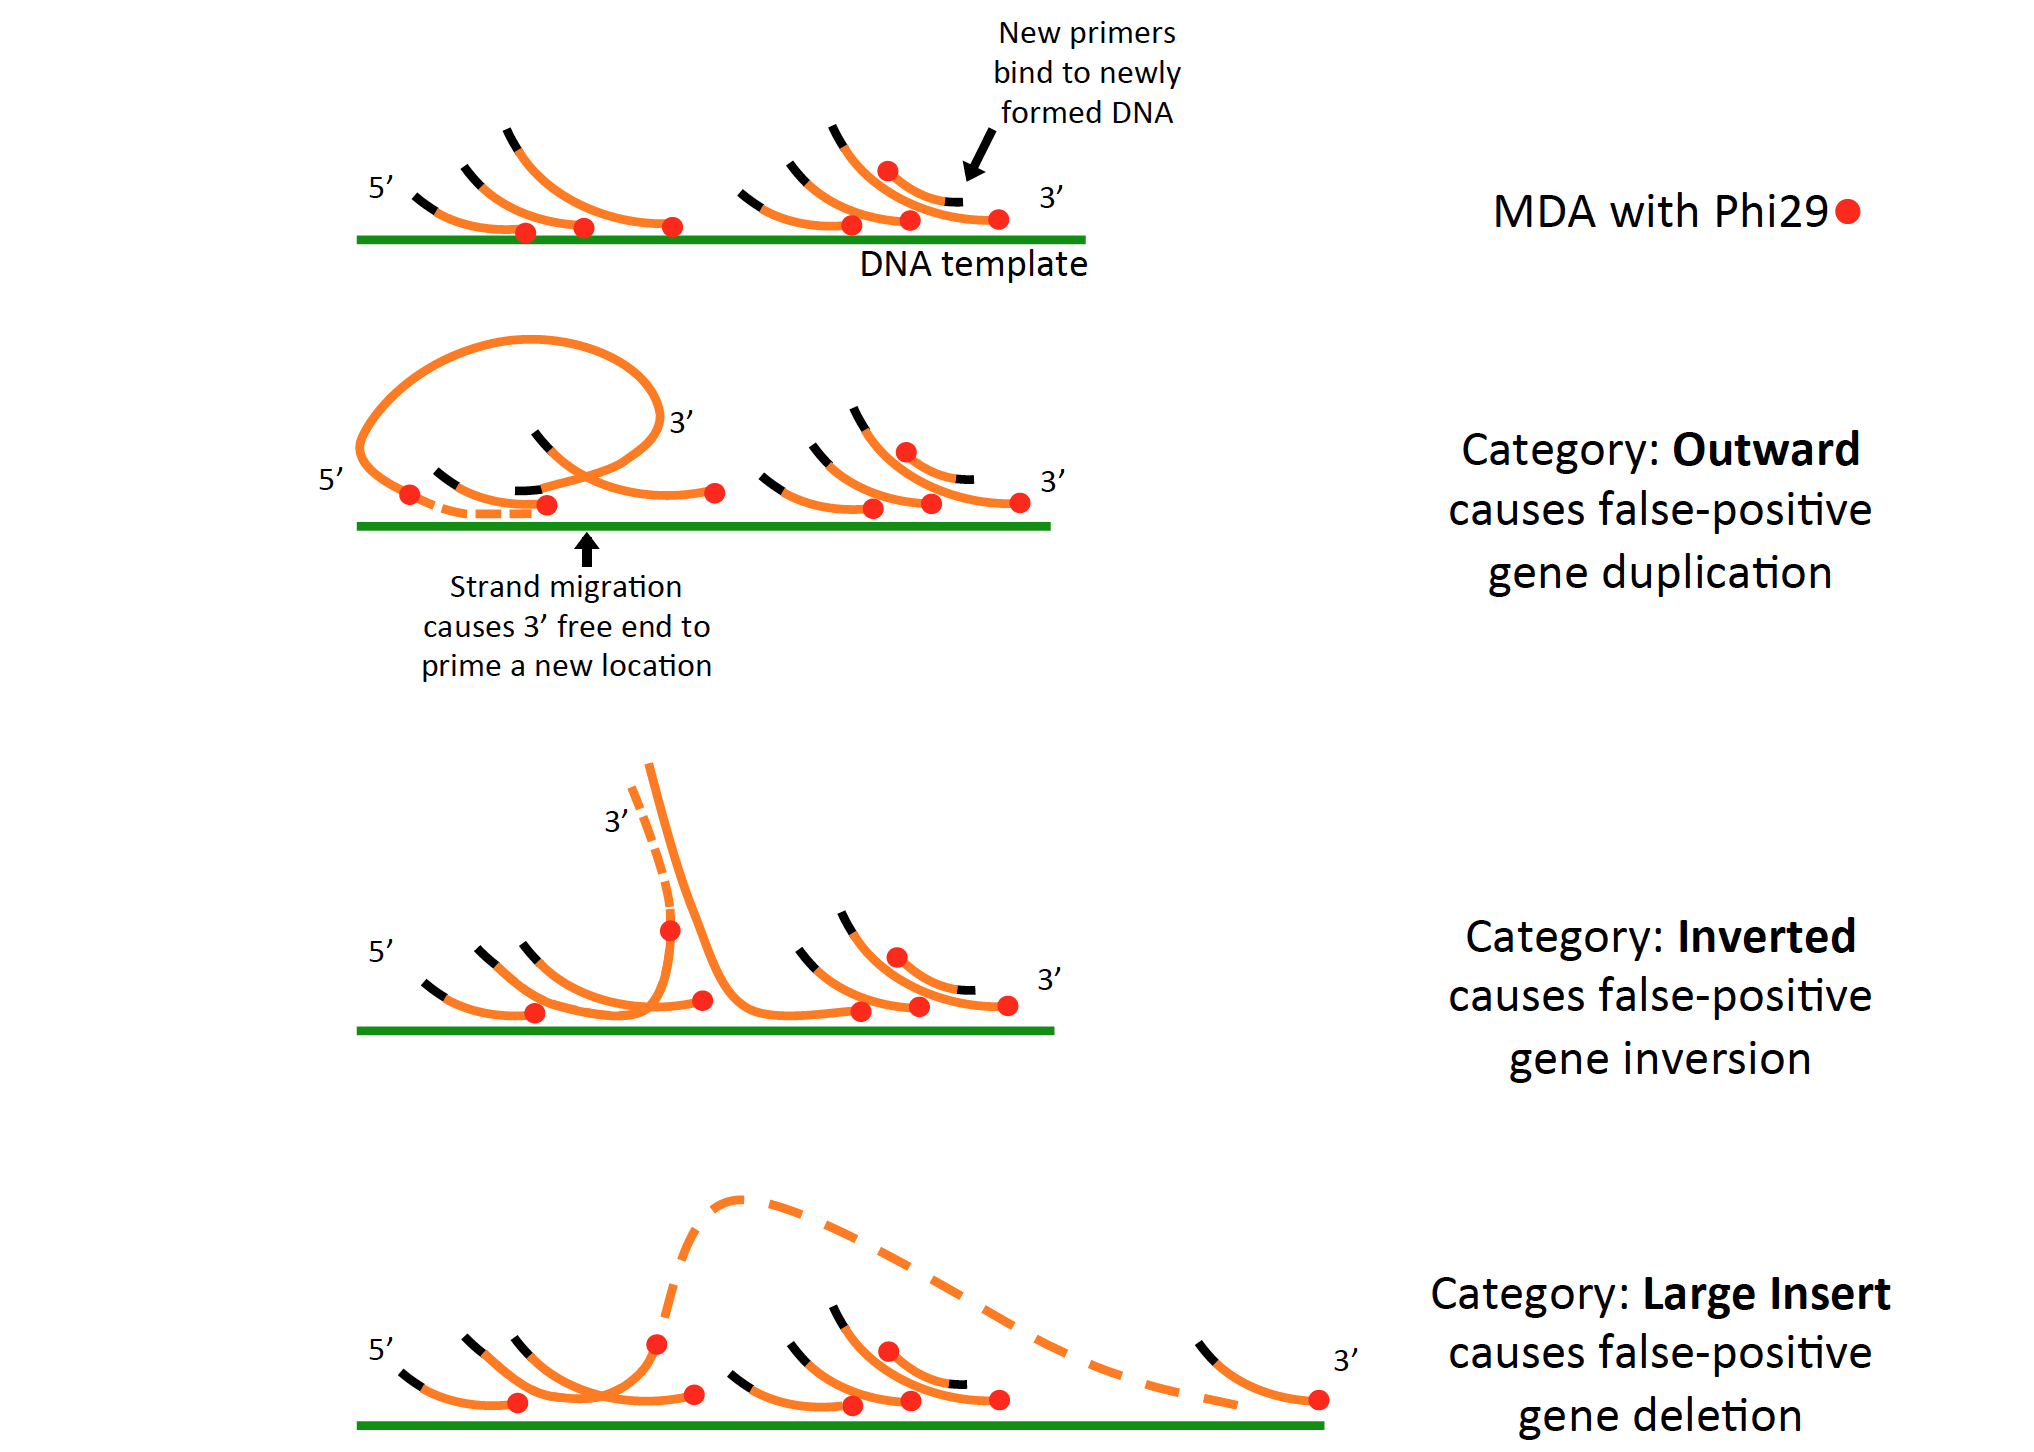
\includegraphics[keepaspectratio,width=1\textwidth]{./figures/ChimeraMechanism}
\caption[The mechanism of MDA chimera]{The mechanism of MDA chimera. The strand displacement action of MDA is shown on top. The strand migration dynamic causes the 3' end to freely bind to another part of the genome, resulting in outward, inverted and large-insert chimera. Cross-chromosome chimera is not shown but the mechanism is similar.}
\label{fig:chimeraMech}
\end{figure}

The data quality of single amplified and sequenced cells is a key to providing accurate and trustworthy information for above-mentioned applications. During the genome amplification and library preparation steps, artifacts are often generated that confound the detection of genomic signatures and complicate data analysis. These artifacts are often due to the implementation of the multiple displacement amplification (MDA) reaction and PCR-based sequencing library preparation \cite{Lasken:2007db}. One type of artifact generated by MDA--chimeric DNA rearrangements (Fig. \ref{fig:chimeraMech}), caused by the highly branched DNA secondary structures with free 3' ends of single-strand DNA during the reaction \cite{Lasken:2007db}, has raised flags in several single-cell studies. It has been shown that the preimplantation genetic diagnosis guided by single-cell genomics can be affected by false-positive SNVs and structural variations from MDA chimera \cite{VanderAa:2013jz, Voet:2013hk}. Researchers using single neurons to study developmental disorders discovered the complication of the chimera artifacts in identifying novel retrotransposon L1 as the existence of the chimera caused false-positive identifications of structural variations \cite{Evrony:2016du, Evrony:2015it}. This is also a problem for environmental microbes that lack a closely related reference genome. But in this chapter, we focus on human cells.   

% Rodrigue \textit{et al.} looked into the \textit{de novo} assembly of single \textit{prochlorococcus} and found inaccurate assembly from MDA chimera \cite{Rodrigue:2009gc}. Uncharacterized microbes such as \textit{prochlorococcus} don't have a reliable reference genome and it is difficult to screen out DNA rearrangements even with long-range sequencing technologies. 

Experimentally, several studies have made attempts to reduce such chimera artifacts. It has been shown that nanoliter microfluidic device might generate less MDA chimera than microliter samples \cite{Marcy:2007il}. However, nanoliter to picoliter microfluidic devices often require clean-room fabrication and supporting pneumatic instruments, which makes it hard to implement for labs with limited resource and funding. Zhang \textit{et al.} used a combination of $\Phi$29 polymerase debranching, S1 nuclease digestion and DNA polymerase I nick translation to reduce the chimeric rate in the library preparation step for single microbes \cite{Zhang:2006hq}, but such methods do not directly affect the chimera generated during MDA reaction. A recent study by Picher \textit{et al.} used a modified $\Phi$29 enzyme for whole genome amplification but didn't show evidence of reduced chimera compared to using unmodified $\Phi$29 \cite{Picher:2016ki}. A novel single-cell technology that is highly accessible and provides high-quality data, especially on reducing the MDA chimera artifact, is greatly needed. 

Bioinformatically, the majority of single-cell studies have focused on characterizing coverage uniformity, CNVs, SNVs, purity and throughput metrics, but have often neglected to quantify the amount of artifacts generated from single-cell whole genome amplification process and sequencing library preparation steps that affect assay performance. There exist established bioinformatic tools designed to filter chimera artifacts from 16S PCR reactions (comparing the phylogenies of fragments) \cite{Edgar:2011gy, Haas:2011jg} and single-cell RNA-seq experiments (with the matching of unique molecular identifiers and cell barcodes) \cite{Dixit:2016ki}. However, existing tools are not designed for chimera characterization and filtering in single MDA-amplified human genomes. A detailed bioinformatic characterization of MDA chimeras is needed to evaluate single-cell technologies and datasets that have been developed and produced. 

\begin{table}
\caption{Single-cell technology comparisons for chimera analysis}
\label{tab:chimeraTechTable}
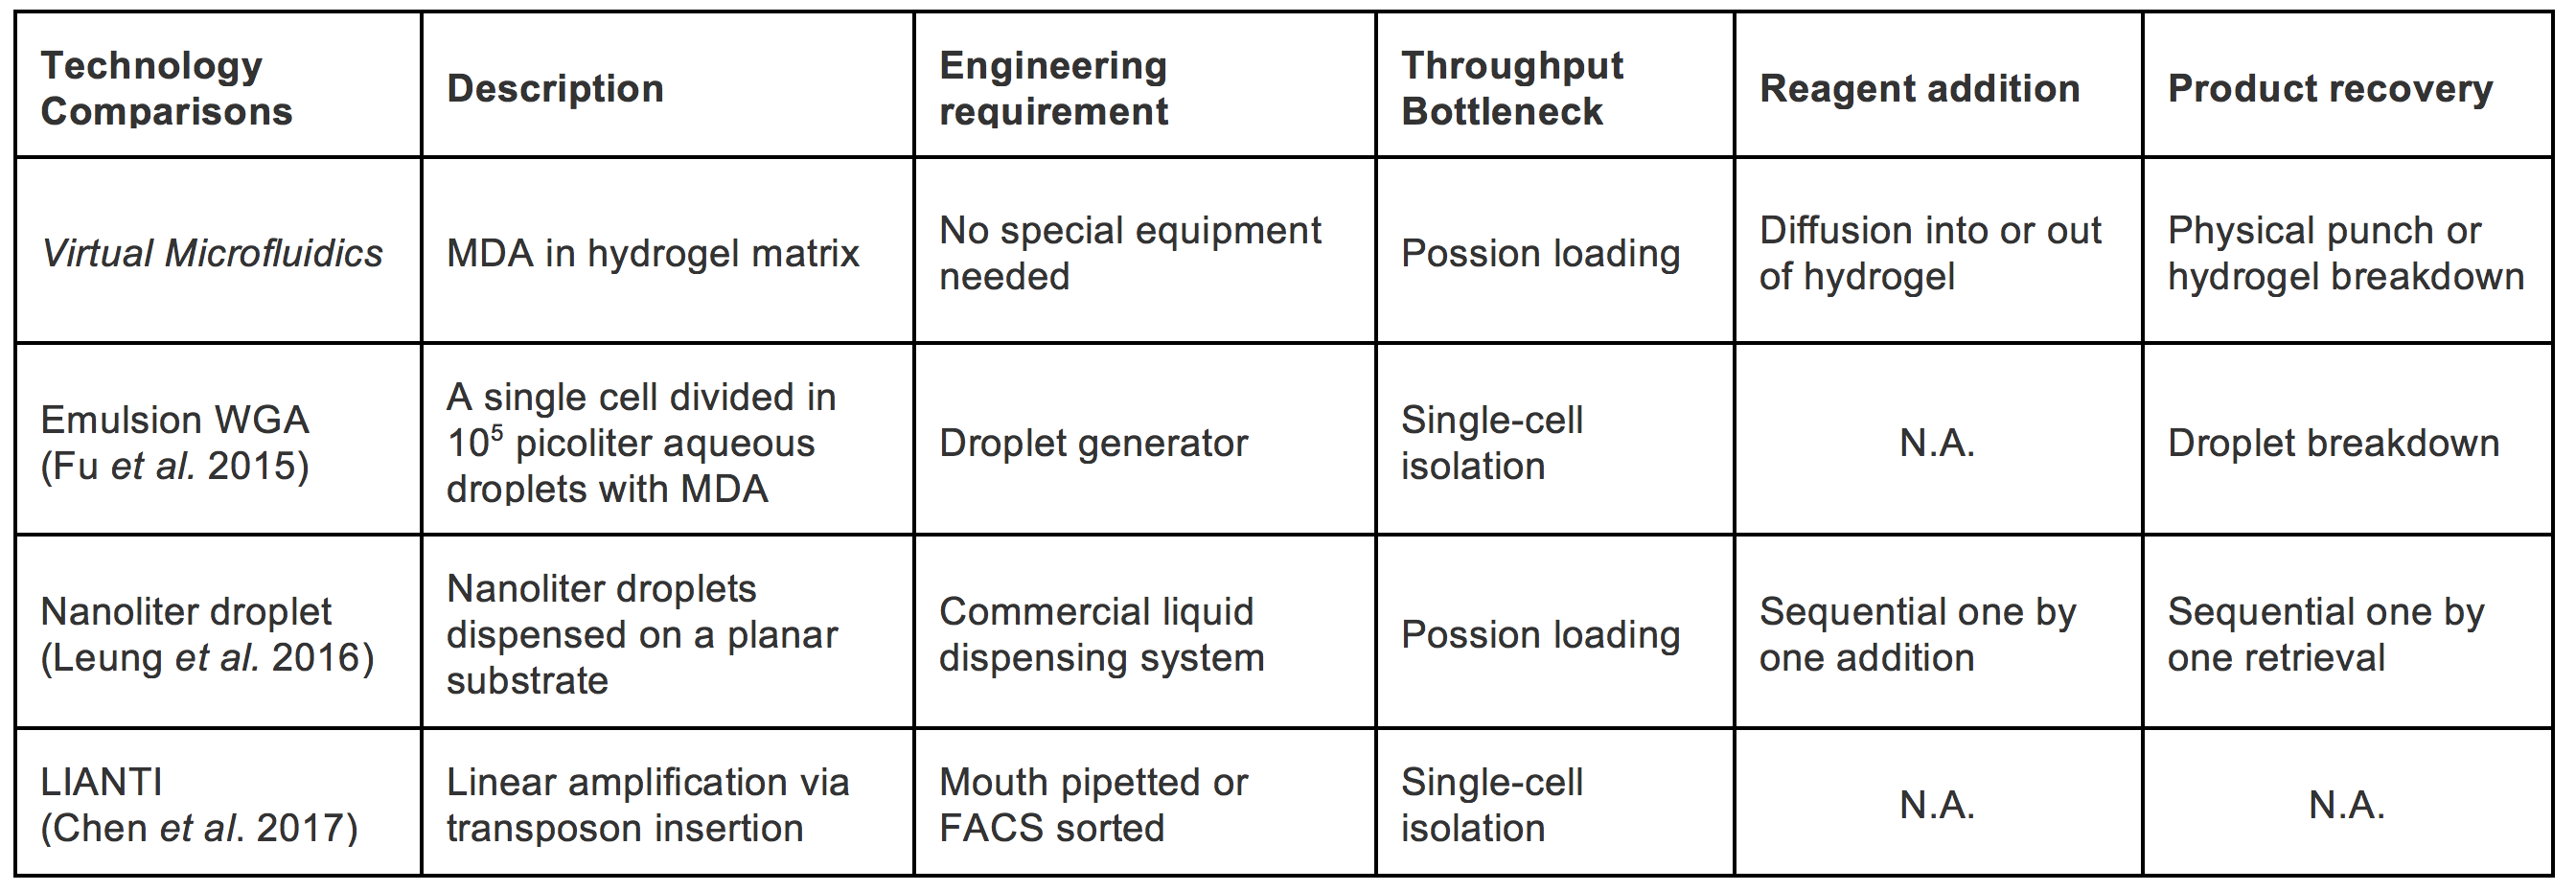
\includegraphics[width=\linewidth]{./figures/Chimera_TechTable}
\end{table}

In this study, we present the application of \textit{virtual microfluidics} on single human cells to demonstrate our technology's capabilities in producing high-quality single amplified human genomes with minimum equipment requirement. We benchmarked its performance with recent innovations of single-cell technologies (Table \ref{tab:chimeraTechTable}) based on exponential amplification method---MDA (eWGA, Nanodrop) and quasi-linear amplification method---LIANTI and MALBAC \cite{ Zong:2012bs,Fu:2015gl,Leung:2016vx,Chen:2017hq}. \textit{Virtual microfluidics} has been shown as a hydrogel-based single-cell isolation and amplification technology that is highly accessible and can provide high-quality single-cell whole genome amplification (WGA) product on cultured bacteria and human gut microbiome samples \cite{Xu:2016wt}. We have previously demonstrated its advantages on small genomes (bacteria) in terms of multi-fold chimera reduction and coverage uniformity improvement. Our hypothesis is that the single amplified human genomes in \textit{virtual microfluidics} will have a similar level of high-quality data to the previous study, with reduced chimeric DNA rearrangements and improved coverage uniformity. 

\begin{figure}
\centering
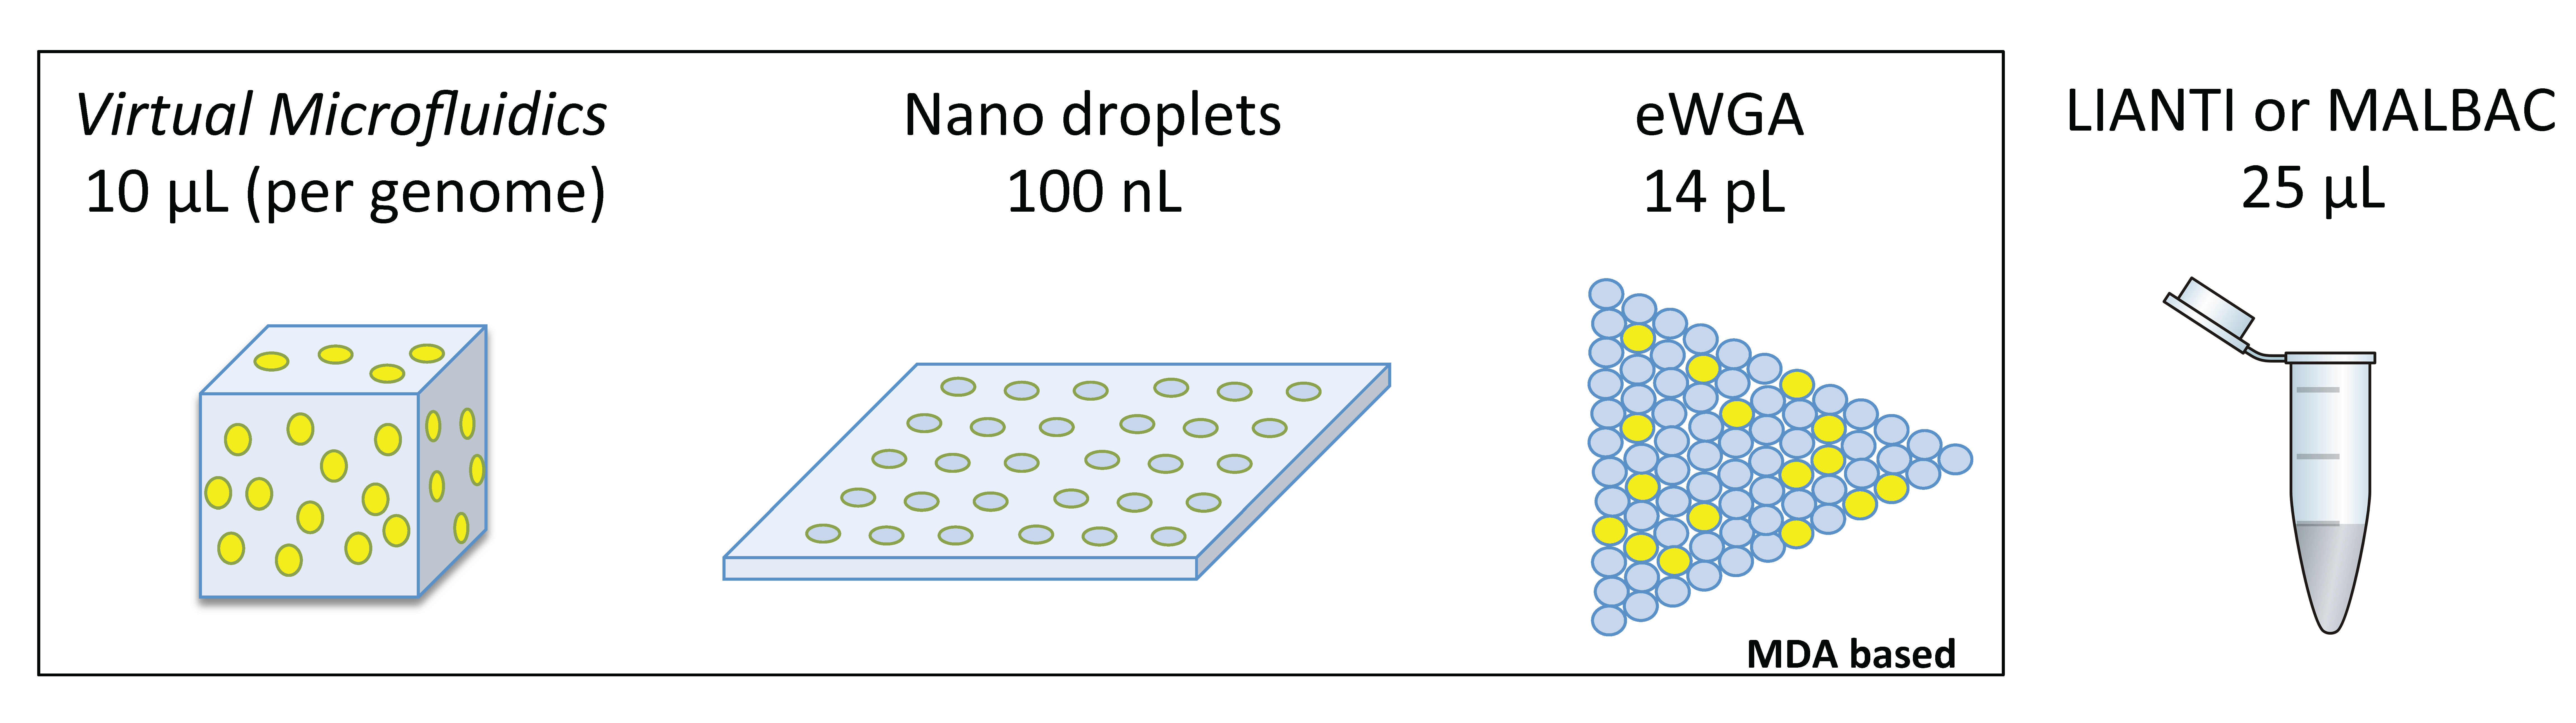
\includegraphics[keepaspectratio,width=1\textwidth]{./figures/Chimera_F1a_TechComparision.png}
\caption[Comparison of single-cell technologies]{Comparison of single-cell technologies. The volume labeled is for each single-cell genome amplification reaction.}
\label{fig:chimeraTech}
\end{figure}

As we mentioned in Chapter 3, the restricted diffusion of the MDA intermediates prevents cross-priming by isolating each portion of the product mixture. It limits cross-chromosome artifacts and chimera reads of large insert size (the distance between the forward read and reverse read mapped on the genome, $\Delta$ mapped coordinates + the length of reverse read). The hydrogel's micro-environment also physically limits the secondary DNA structures during MDA, thus reducing the chimera breakpoints out of total reads that are pair-mapped. To support the technology demonstration, we developed an algorithm to categorize the signatures of MDA chimeras across multiple single-cell platforms. This characterization will serve as a guidance for chimera analysis to be a non-negligible part of the analysis suite for evaluating future single-cell technologies.  

\section{Results and Discussion}
%%The discussion needs to draw comparative conclusions more directly (not just make qualitative general statements) from the data and describe the statistical support for these conclusions. The discussion should also tie back to the applications with some recommendations of what methods to use for which types of studies. There are still a number of typos and grammatical issues to clean up
We conducted modified \textit{virtual microfluidics} single-cell sequencing on 8 RPE--1 cells in a HiSeq 2500 lane with 2$\times$125 and obtained roughly 1$\times$ mapping depth to reference genome GRCh37-lite (methods). We characterized the single RPE cell dataset while benchmarking with unsorted\slash (unclear whether cherry-picked) single-cell datasets from eWGA (5 cells), MALBAC (2), tube MDA (2), Nanodrop (9) and LIANTI (3) (Table \ref{tab:chimeraDataSource}, Table \ref{tab:SRAaccession} and Fig. \ref{fig:chimeraTech}). All samples were trimmed and analyzed according to the analysis workflow (Fig. \ref{fig:chimeraWorkflow}). All mapped, de-duplicated, repeat-masked and sorted BAM files are down-sampled to 430,000 reads\slash sample ($\sim$0.01$\times$, including both forward and reverse reads) for chimera analysis (methods) . 

\begin{table}
\caption{Data source for chimera analysis}
\label{tab:chimeraDataSource}
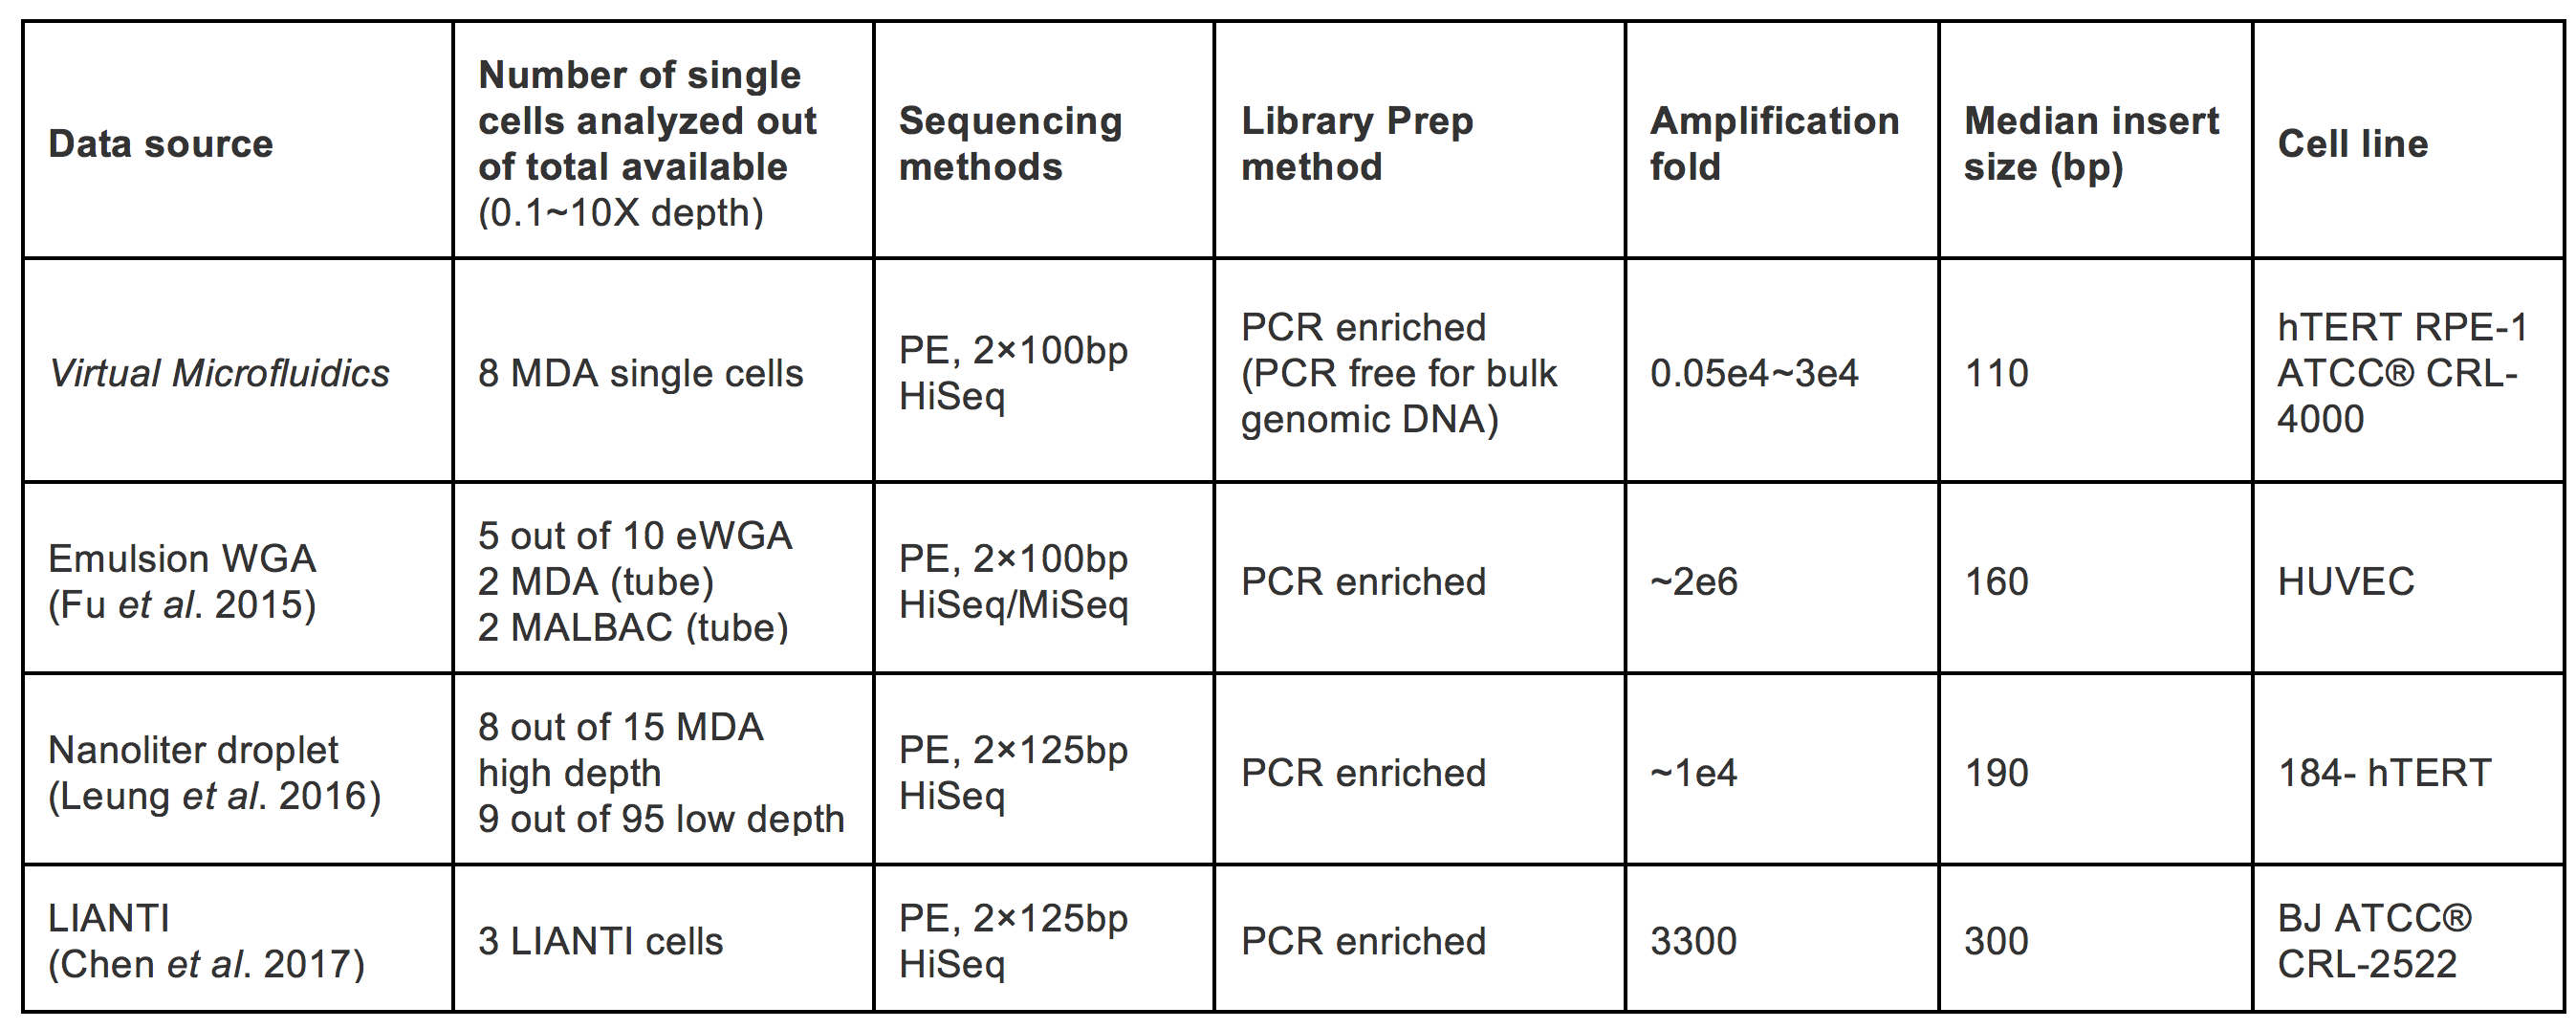
\includegraphics[width=\linewidth]{./figures/Chimera_DataTable}
\end{table}

The benchmarking datasets were chosen to represent different methods of cell isolation (hydrogel-based \textit{virtual microfluidics}, emulsion droplets, liquid dispensing), WGA chemistry (MDA, MALBAC, LIANTI) and library preparation methods (Nextera PCR-enriched and PCR-free ligation-based). According to Evrony \textit{et al.} 2015, most chimera originated from library preparation after MDA reaction. However, our previous study showed a multifold chimera rate reduction from MDA process in cultured bacteria compared to standard tube reactions using the same library preparation procedure (Nextera). Including above-mentioned datasets will help parse out the chimera characteristics and sources from single amplified human genomes. 

\begin{figure}
\centering
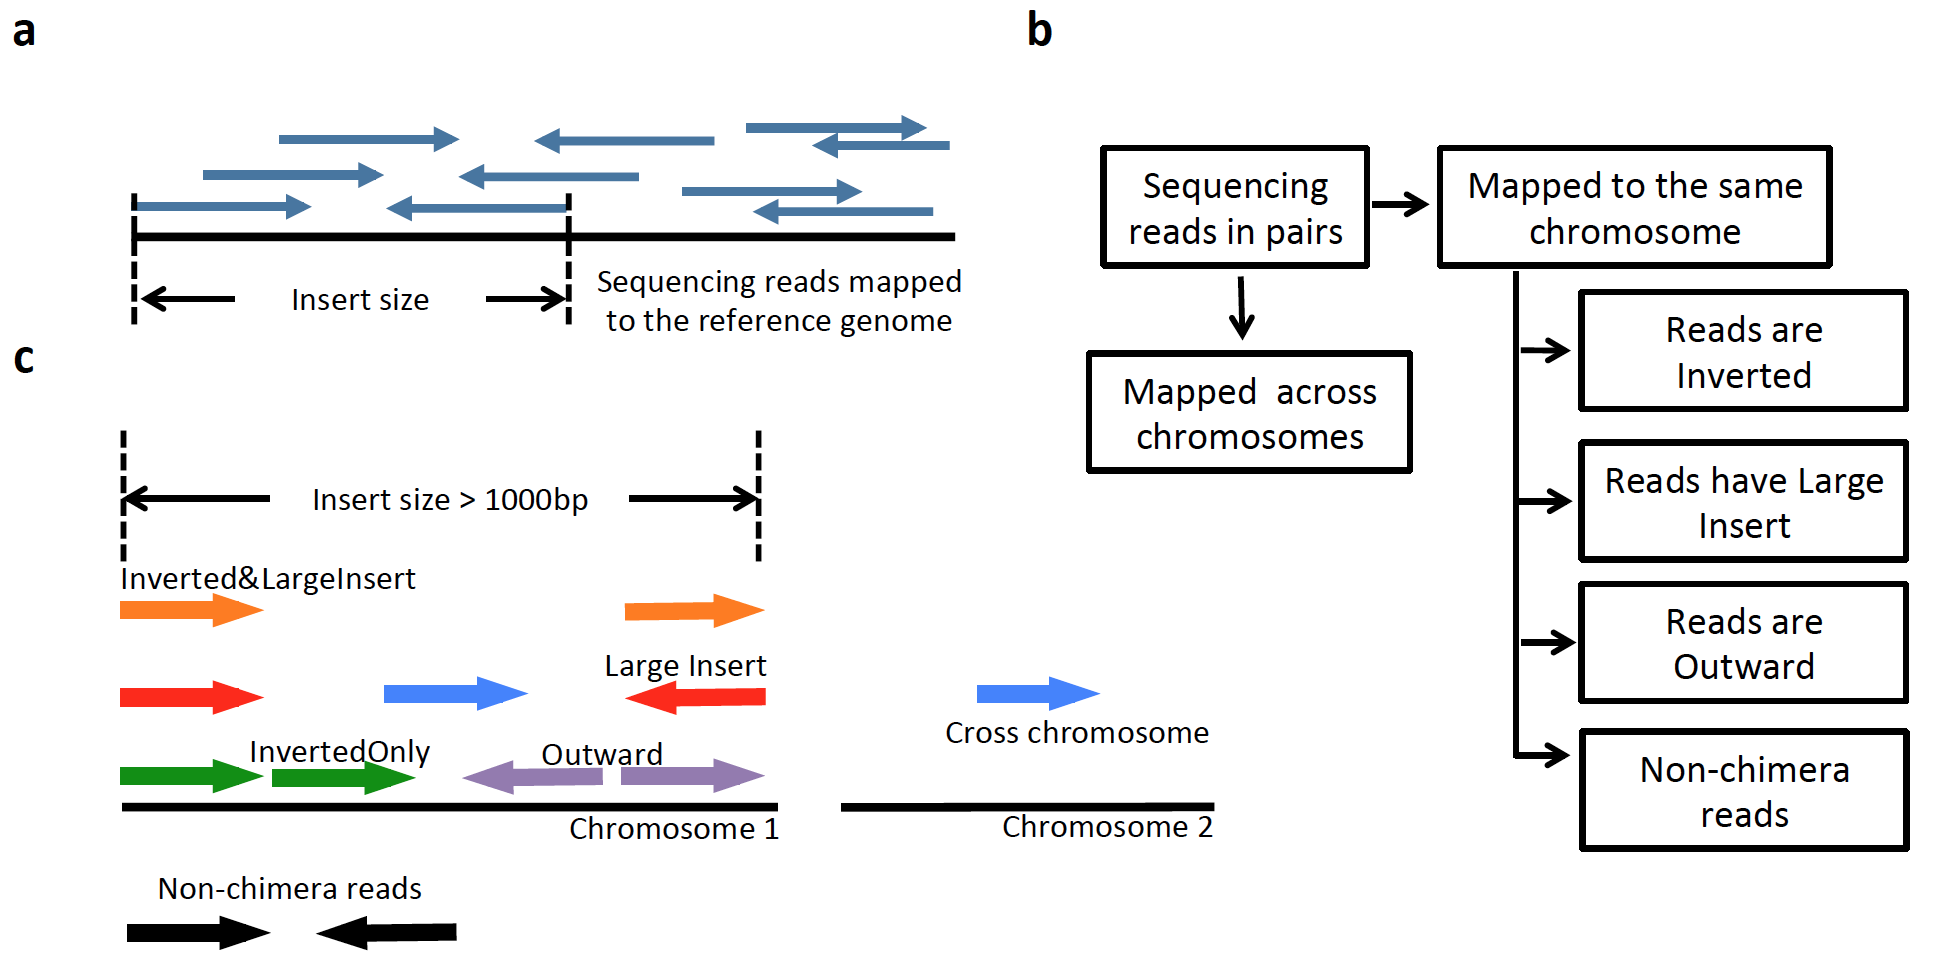
\includegraphics[keepaspectratio,width=1\textwidth]{./figures/ChimeraCategories_cropped}
\caption[Pair-ended sequencing for the chimera categorization.]{Pair-ended sequencing provides read orientations for the chimera categorization. (a) The insert size represents the length of DNA fragment. (b) The decision workflow to categorize different chimera reads. (c) Chimera and non-chimera reads are illustrated.}
\label{fig:chimeraWorkflow}
\end{figure}

It has been shown from a couple hundred sequencing reads of \textit{E. coli} that over 85\% of MDA chimeras are inverted read pairs, which means the forward and reverse read pairs don't have the correct orientation (inward facing) \cite{Lasken:2007db}. This type of sequencing result can be easily filtered out in a single-chromosome organism with the well-established reference genome, such as culturable bacteria. However, it becomes bioinformatically difficult when the reference genome is enriched with repeat islands in mammalian cells and when the draft genome is often inaccurate for unculturable environmental microbes. Making improvements in single-cell technologies is a task that needs to be done well both experimentally and bioinformatically. 

\subsection{Chimera categories}
A correct read pair should map to different strands (+/-, or sense and antisense) within the insert size range controlled by sequence library size selection (200 bp $\sim$ 800 bp). We defined five categories of chimera reads in this study (Fig. \ref{fig:chimeraWorkflow}b&c). Inverted means forward and reverse reads mapped to the same strand of DNA template (Fig. \ref{fig:chimeraWorkflow}c).  Within the inverted reads categories, the pairs of reads can be further categorized into inverted\&LargeInsert (>1000 bp insert size) and InvertedOnly (<1000 bp). For reads with the correct orientation, the pairs of reads can be categorized into LargeInsert Only chimera (>1000 bp) and cross-chromosome chimera. The color code in Fig. \ref{fig:chimeraWorkflow}c corresponds to the same categorizations in Fig. \ref{fig:chimera5Categories} chimera quantification. The five categories are mutually exclusive and collectively exhaustive for all chimeras that can be parsed out. 

\begin{figure}
\centering
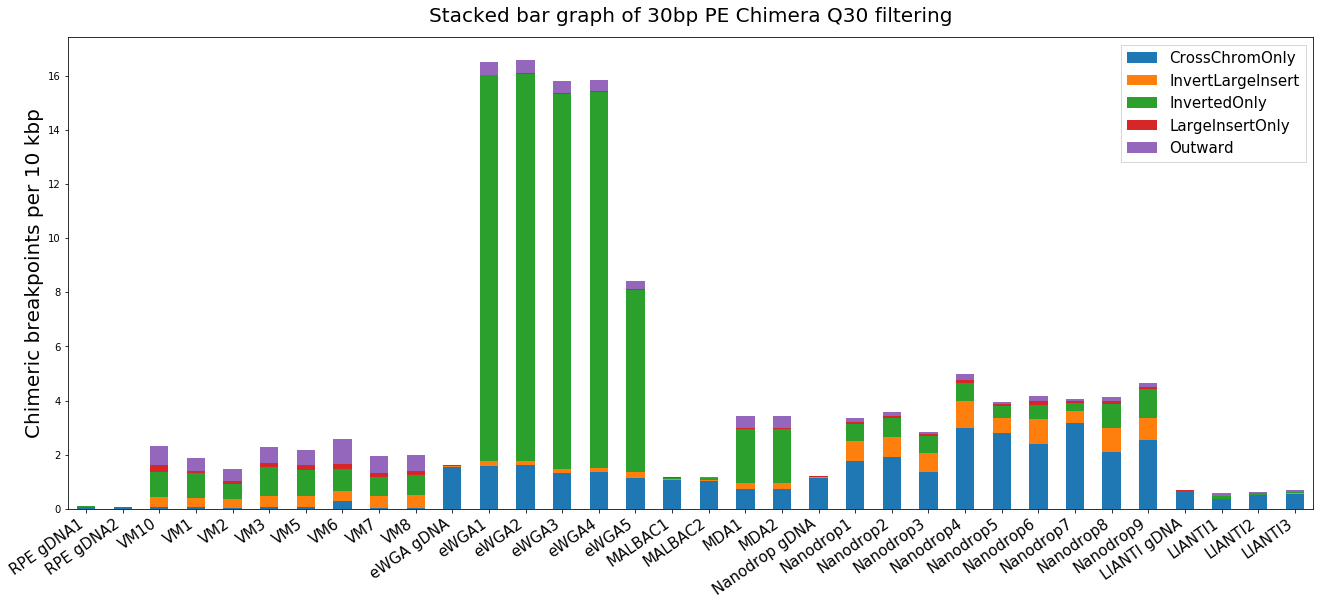
\includegraphics[keepaspectratio,width=1\textwidth]{./figures/20170727_ChimeraSubcategories_IScorrected_PE_30bp_Q30}
\caption[Chimeric breakpoints per 10 kbp]{Chimeric breakpoints per 10 kbp across all samples are shown as 5 categories of chimera: cross-chromosome, inverted, large insert size (>1000 bp), outward, and inverted large insert.}
\label{fig:chimera5Categories}
\end{figure}

The median insert size distribution of sequencing reads across different datasets varies from 100 bp $\sim$ 300 bp. In order to eliminate the factor of inconsistent insert size on chimera detection and possible read overlaps, we normalized the chimera breakpoints over total basepairs mapped and trimmed all sequencing reads to 30 bp \cite{Tu:2015dc}. Previous studies have revealed the nature of MDA chimera in terms of overlapping number of basepairs in the chimera junction \cite{Tu:2017fz, Tu:2015dc}. Here we focus on the categorization of MDA chimera in different single-cell whole genome amplification technologies on human cells and their genome-wide signatures. Single-ended and pair-ended mapping of the same sequencing dataset were implemented side by side to compare the read paring's impact on chimera detection. Here we define the chimera breakpoints as the total number of Read 1 and Read 2 that categorize as chimera reads (as there are two parts of the genome joined together, which represents two breakpoints). 

\begin{eqnarray*}
\text{Chimera breakpoints per 10 kbp} = \frac{ \text{Chimera reads } (R1 + R2) \times 10^4}{ \text{Total number of bp mapped}} \\
\\
= \frac{ \text{Chimera reads } (R1 + R2) \times 10^4}{ (\text{Total pairs of reads that are mapped}) \times \text{Average insert size}}
\end{eqnarray*}

Fig. \ref{fig:chimera5Categories} shows the number of chimeric breakpoints per 10 kbp mapped in a stacked bar graph. Genomic DNA (gDNA) samples without WGA serve as the baseline of comparisons. \textit{Virtual microfluidics} samples exhibit low chimera breakpoint frequency while confirming the 85\% inverted composition in MDA chimera. RPE gDNA was processed with PCR-free library preparation and is used as the negative control of chimera detection. The residual chimera detected from the RPE gDNA represents the inherent genome structural variations of the cell line. This also serves as the comparison for the chimera introduced by PCR library preparation process. The eWGA, Nanodrop, and LIANTI gDNA all went through PCR enrichment. But it is unknown whether these 3 cell lines used (PCR-free datasets unavailable) have inherently higher structural variations than RPE cell line does. 

Interestingly, the eWGA single cells show more than 90\% enrichment in \say{Inverted Only} chimera reads and a 3 $\sim$ 7 fold chimera frequency increase compared to the gDNA baseline. This increase can be explained by the isolation of individual fragments in picoliter liquid droplets. The confinement of a single DNA template in picoliter volume resulted in mostly inverted artifacts from MDA while few template was available for cross-chromosome priming to happen. The nanodrop dataset has a different pattern for chimera signature, showing more than 50\% chimeras that span across different chromosomes and 25\% chimeras with large insert size. Both eWGA and nanodrop methods have a higher frequency of chimera reads occurrence compared to microliter-ranged in-tube MDA. Our explanation is that a smaller reaction volume does not affect the secondary structure of a single-strand DNA. But a higher density of DNA increases the chance of cross priming. Due to the smaller reaction volume that increases the DNA density in the reaction, more chimeras are produced in eWGA and Nanodrop. 

%This finding contradicts to the previous study that claimed "nanoliter microfluidic device might generate less MDA chimera than microliter samples".

% \begin{figure}
% \begin{tabular}{lc}
% (a) \\
% \includegraphics[keepaspectratio,width=1\textwidth]{./figures/20170517_ChimericBreakpoint10kbp_PE_Qfiltered} \\
% (b) \\
% \includegraphics[keepaspectratio,width=1\textwidth]{./figures/20170517_ChimericBreakpoint10kbp_SE_Qfiltered} \\
% \end{tabular}
% \caption[The effect of mapping quality filtering on chimera detection.]{The effect of mapping quality filtering on chimera detection. (a) Pair-ended (PE) mapping with BWA aligner. (b) Single-ended (SE) mapping with BWA aligner}
% \label{fig:chimeraMappingQ}
% \end{figure}

\subsection{Chimera rate analysis with respect to mapping quality filtering} % (fold)
% subsection subsection_name (end)}
We implemented mapping quality filters (Q = 30, 20, 10) and found a slight decrease of chimera rate when increasing the mapping quality threshold as expected by the more stringent quality filtering (Fig. \ref{fig:chimeraMappingQAll}). 

\begin{figure}
\centering
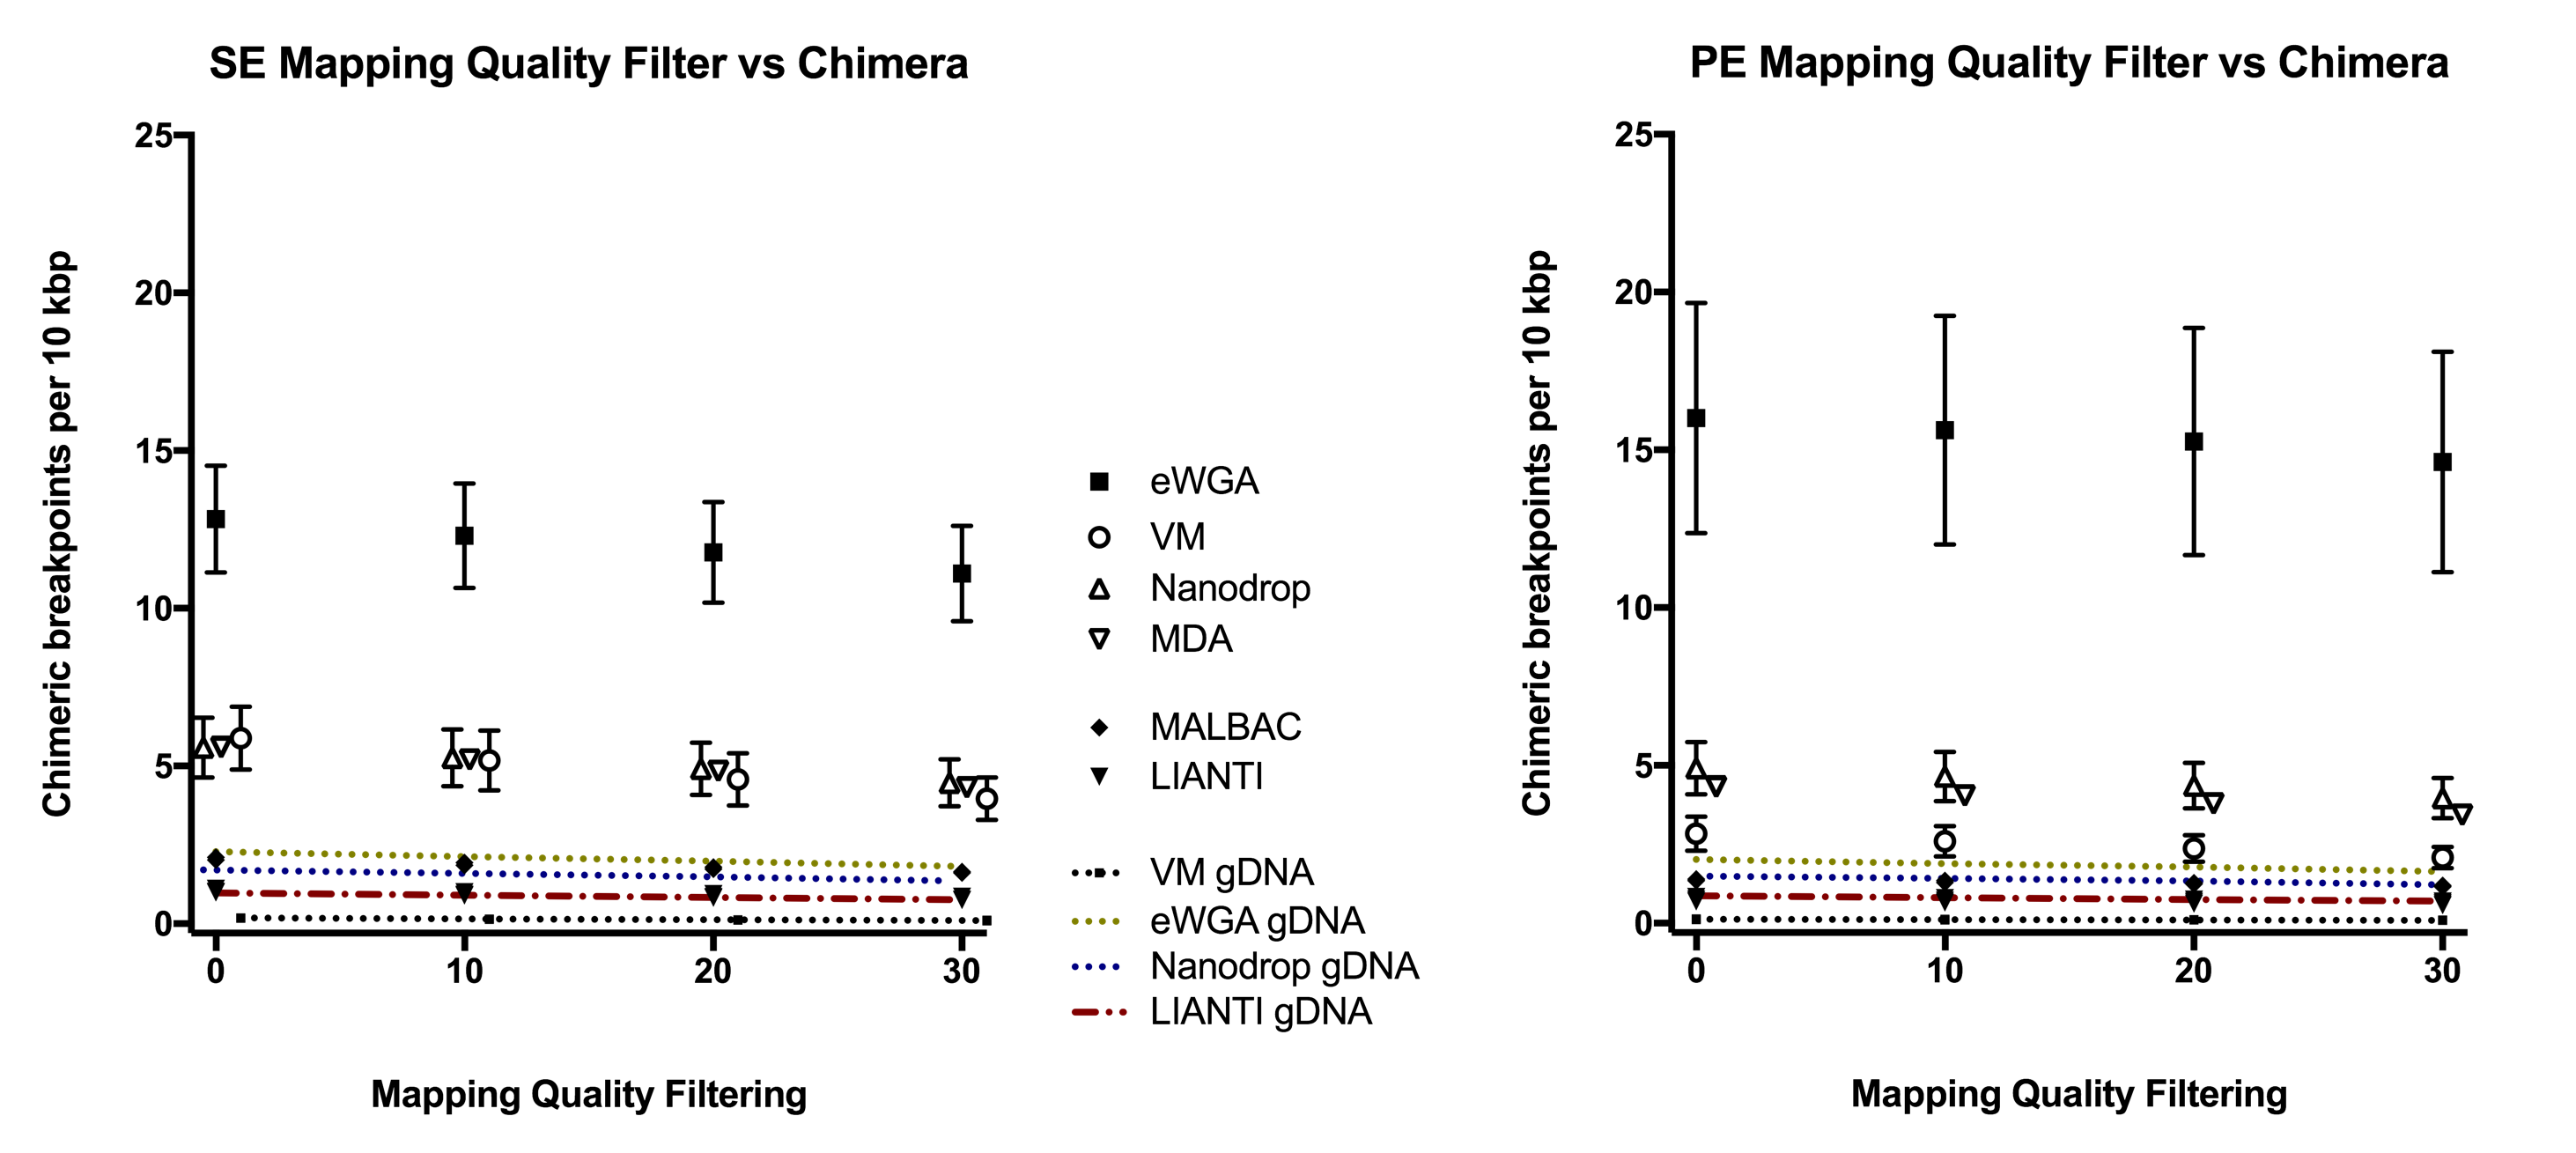
\includegraphics[keepaspectratio,width=\textwidth]{./figures/MappingQvsChimera}
\caption[The effect of mapping quality filtering on chimera detection.]{The effect of mapping quality filtering on chimera detection.}
\label{fig:chimeraMappingQAll}
\end{figure}

\begin{figure}
\centering
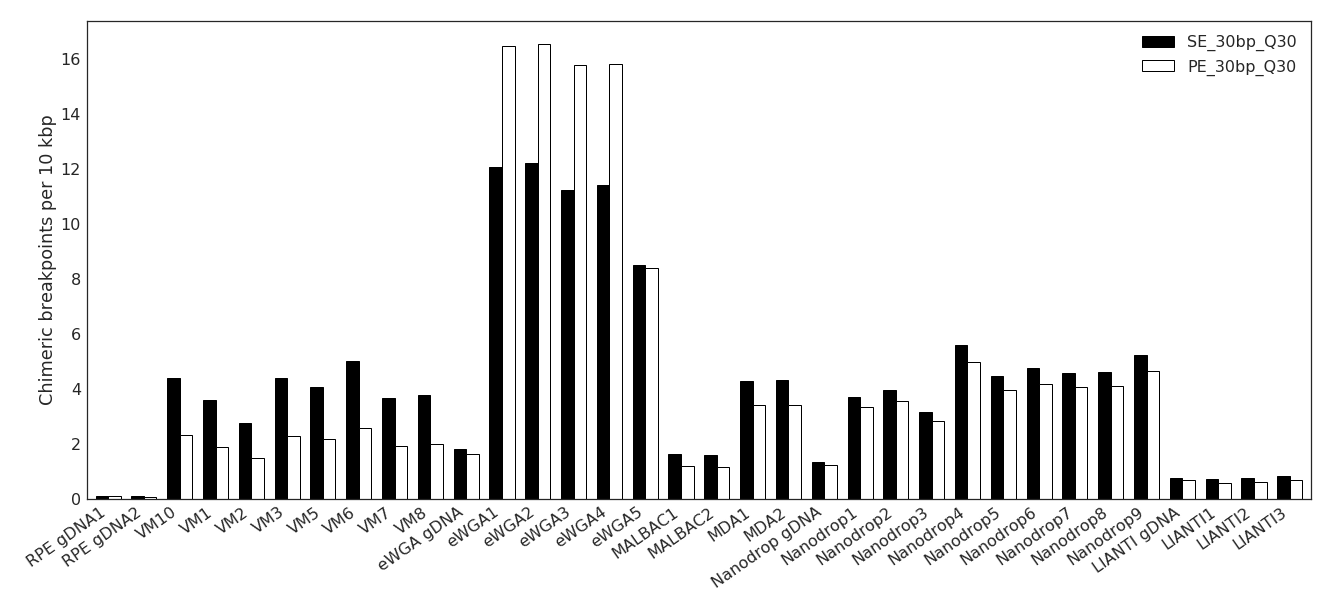
\includegraphics[keepaspectratio,width=1\textwidth]{./figures/20170517_ChimericBreakpoint10kbp_SEvsPE_Q30}
\caption[The effect of pair-ended and single-ended mapping on chimera detection]{The effect of pair-ended (PE) and single-ended (SE) mapping on chimera detection.}
\label{fig:chimeraPEvsSE}
\end{figure}

Most interestingly, we compared the effect of pair-ended and single-ended mapping on chimera detection (Fig. \ref{fig:chimeraPEvsSE}). For all datasets except eWGA, single-ended mapping analysis overestimates chimera rate compared to pair-ended mapping with the same downsampled reads. With pair-ended mapping, read pairs mapped within the range of insert size with the correct orientation is chosen as the primary mapping results. With the single-ended mapping, reads that mapped to multiple locations equally well were randomly chosen for the final output, thus, causing an overestimation of chimeric read out of total mapped reads. For eWGA, there is a 50\% increase of chimera frequency by pair-ended mapping compared to single-ended mapping. This increase can be explained by the especially high content of inverted chimera that can be easily detected in the pair-end mode. In the single-end mode, a potential inverted chimera might be able to map to a reverse-complementary location with the same mapping quality, and thus, the single-end mode underestimate the chimera rate. We are uncertain about why VM samples are affected the most by PE vs SE mapping ($\sim$ 50\% change). Possible explanations include the differences between cell lines, library preparation procedures and the nature of DNA amplification in hydrogel. Further experiments will be needed to validate the cause. 

\begin{figure}
\centering
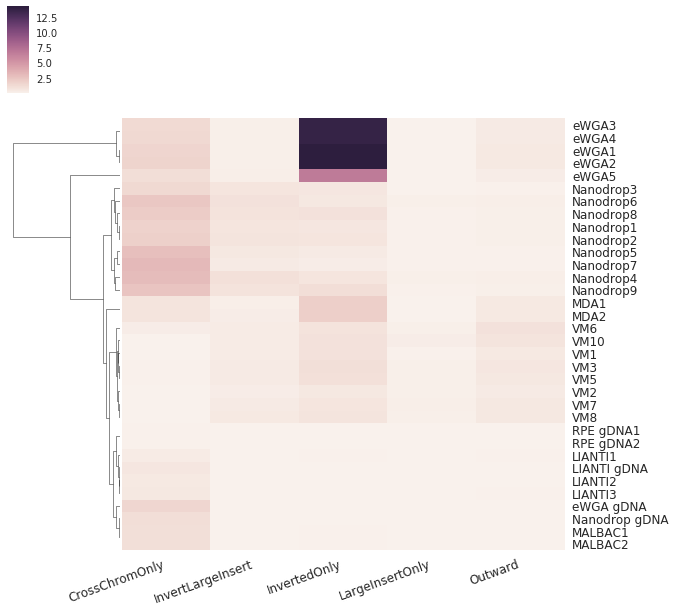
\includegraphics[keepaspectratio,width=1\textwidth]{./figures/20170822_BreakpointPer10kbp_Clustermap_QFiltered}
\caption[Hierarchical clustering of chimera breakpoints per 10 kbp.]{Hierarchical clustering of chimera breakpoints per 10 kbp for each single cells and genomic DNA controls.\textit{Virtual Microfluidics} samples are closely clustered with genomic DNA controls, indicating low levels of chimera generated by hydrogel MDA}
\label{fig:chimeraCluster}
\end{figure}

Furthermore, by hierarchically clustering the datasets based on their chimera signatures (Fig. \ref{fig:chimeraCluster}), we see the close similarities between \textit{virtual microfluidics} samples and the LIANTI single cells in terms of chimera rate, while most of the nanodrop datasets are closely clustered with traditional MDA reactions. MALBAC samples are clustered with gDNA controls with PCR-enriched chimera baseline. LIANTI samples are closely clustered with PCR-free gDNA controls that represent chimera-free negative control, which indicates the \textit{in vitro} transcription amplification could generate minimal chimera. 

% \begin{figure}
% \centering
% 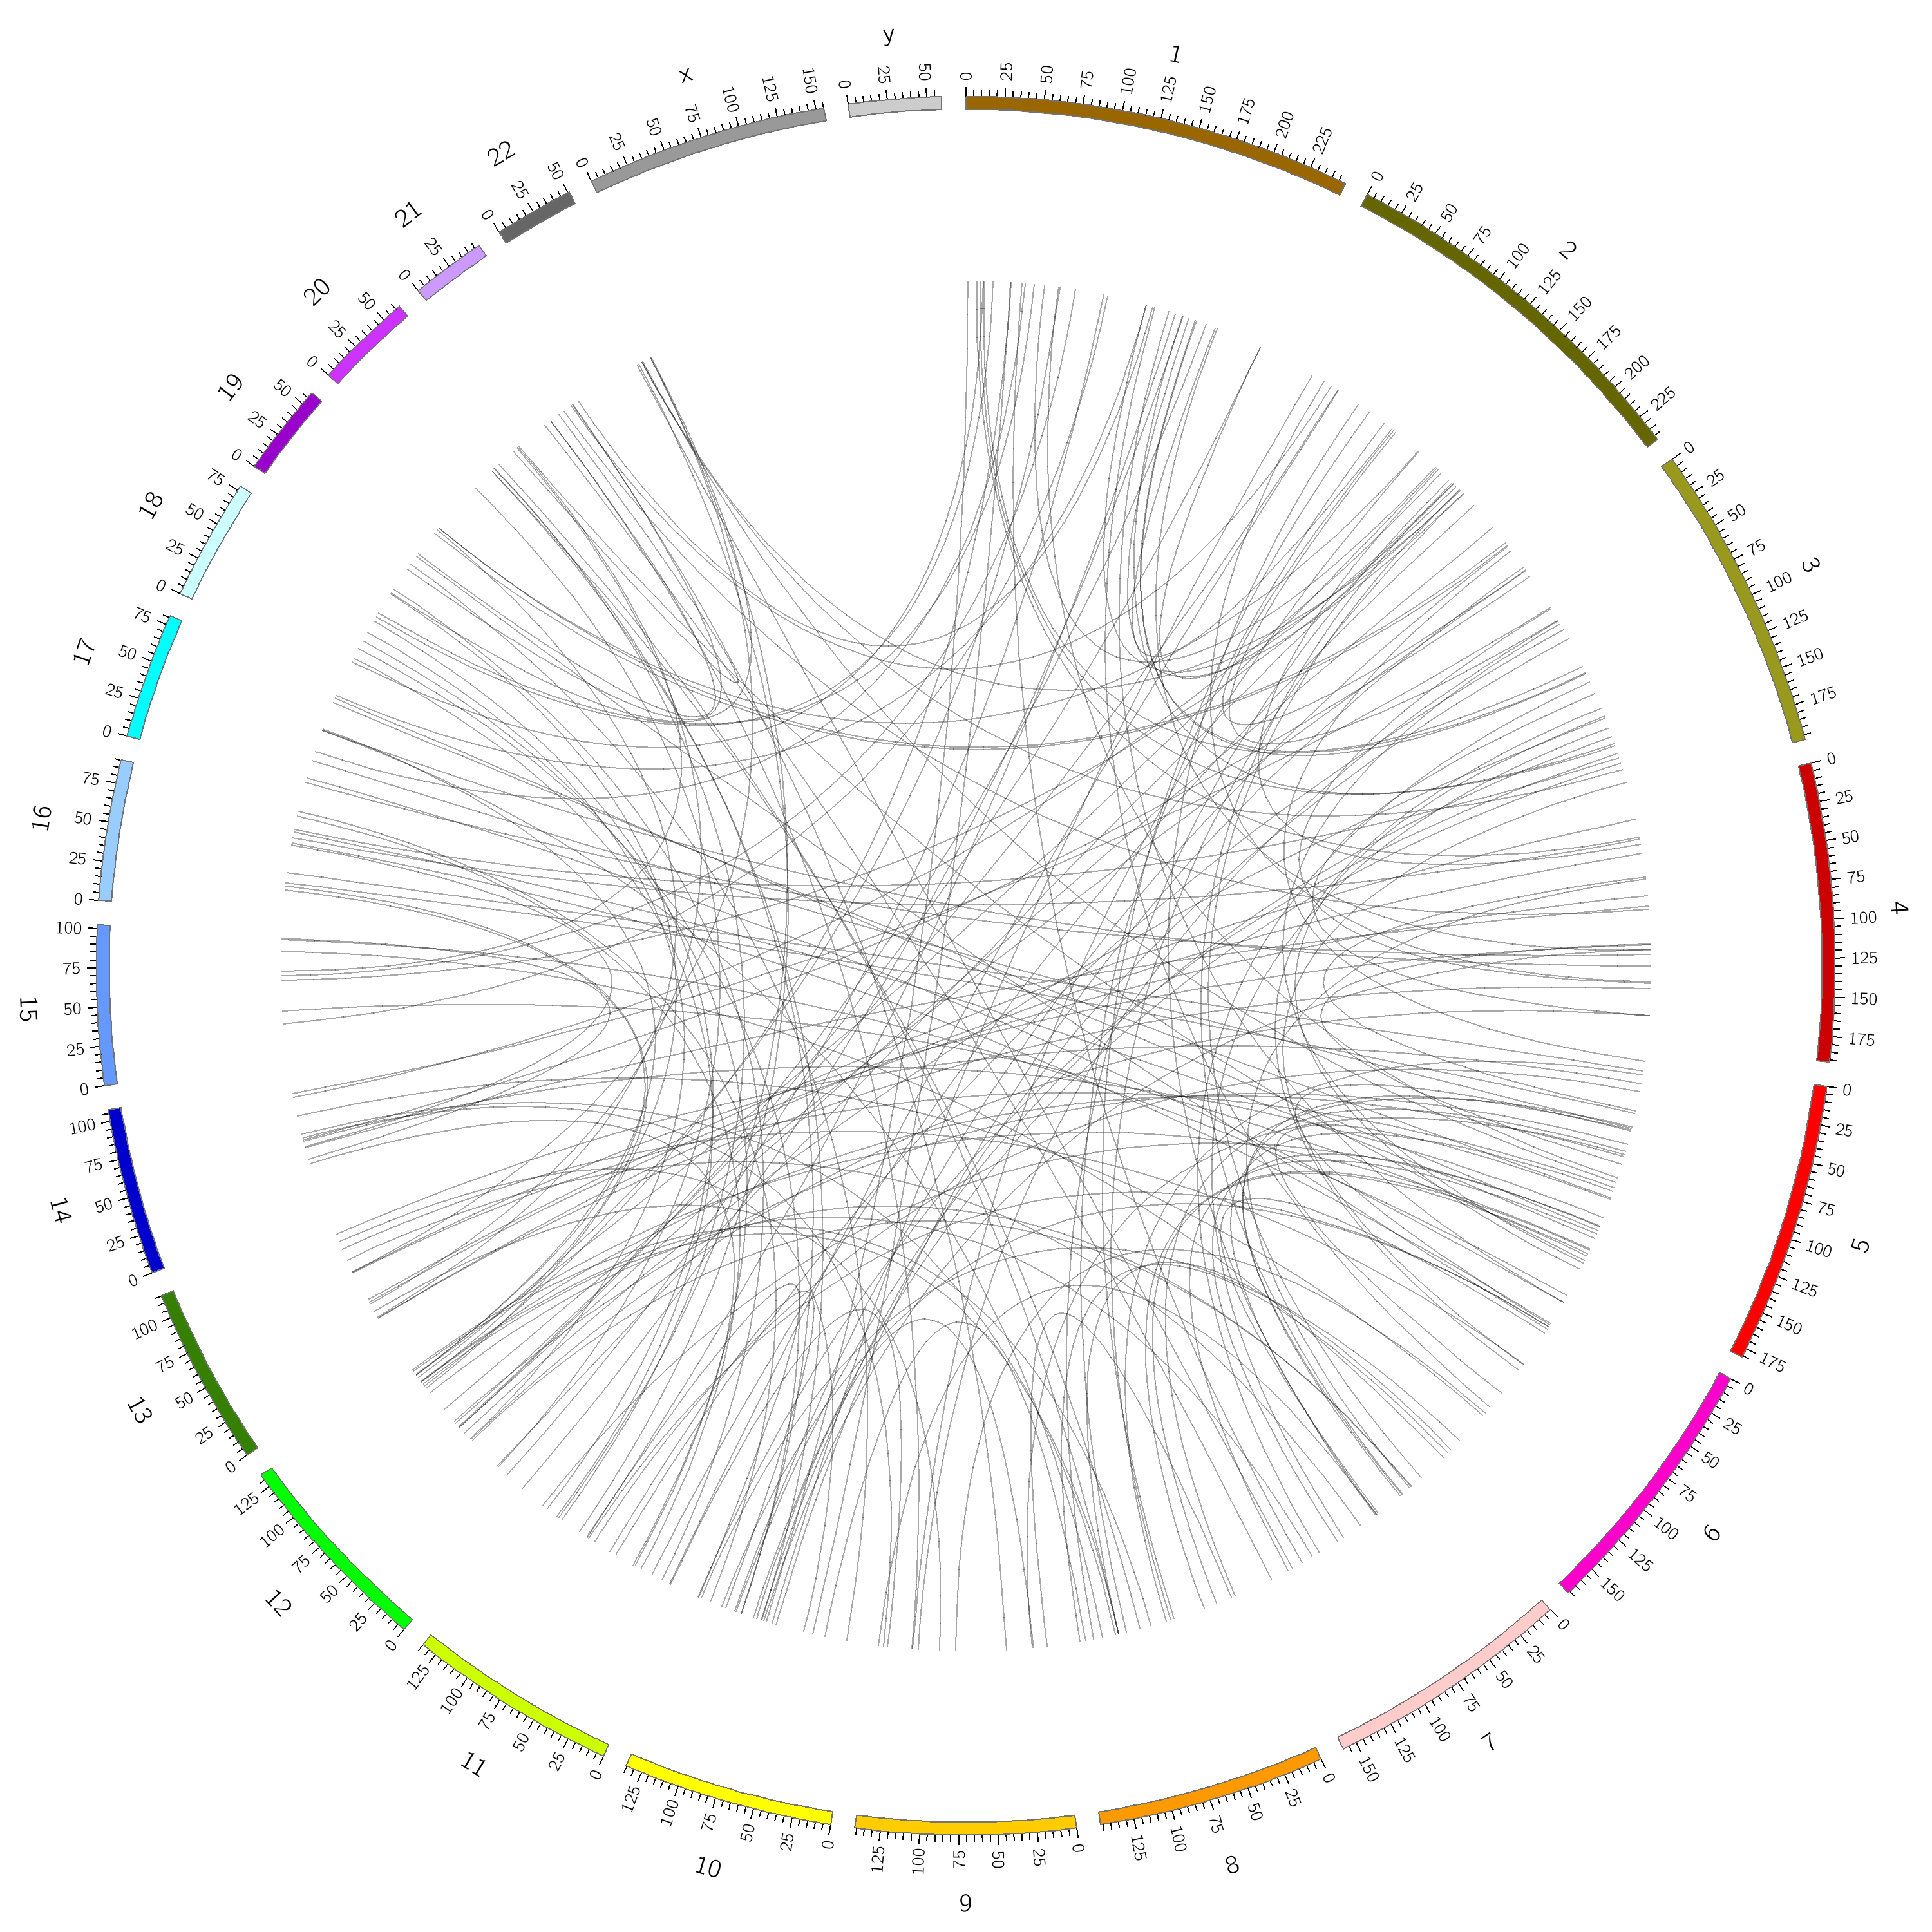
\includegraphics[keepaspectratio,width=1\textwidth]{./figures/LX0gDNAcircos}
% \caption[Cross-chromosome chimera map for RPE genomic DNA]{Cross-chromosome chimera map for RPE genomic DNA. Cross-chromosome chimera pairs are connected, shown as the black lines.}
% \label{fig:LX0gDNAcircos}
% \end{figure}

\begin{figure}
\begin{tabular}{cc}
VM gDNA (PCR free) & VM 1 \\
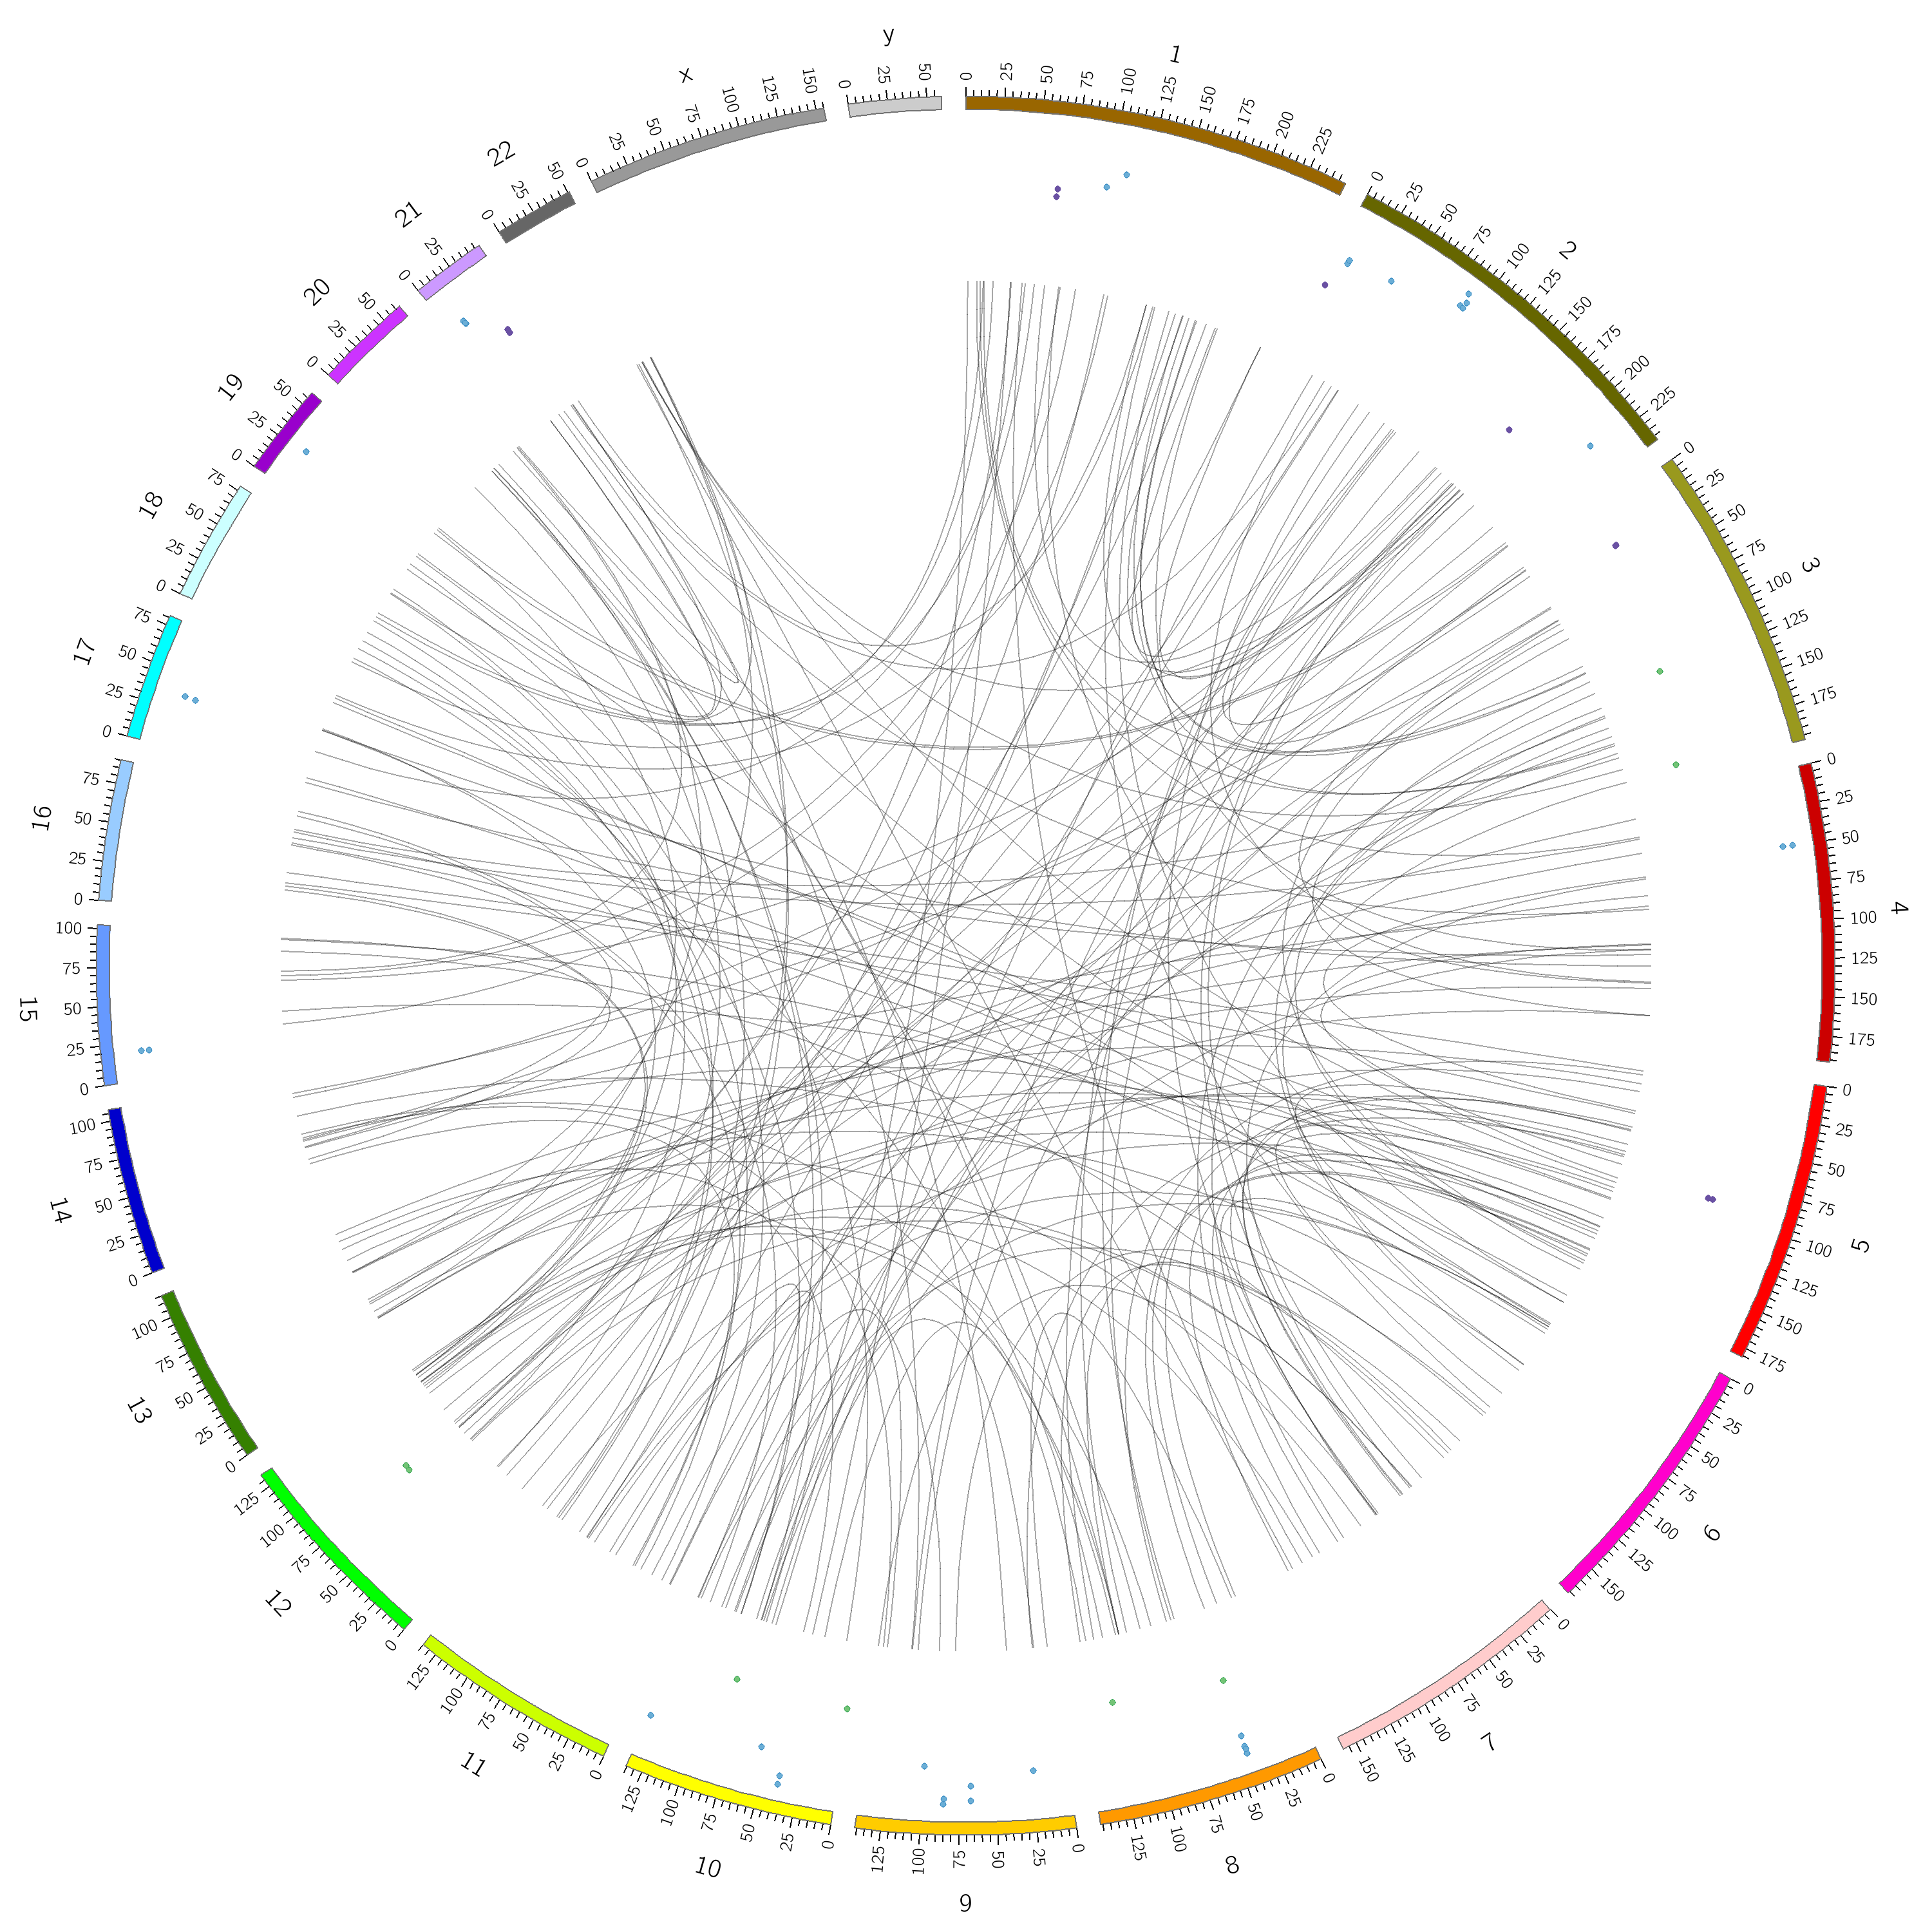
\includegraphics[keepaspectratio,width=0.5\textwidth]{./figures/circos/LX0gDNA_0529} & 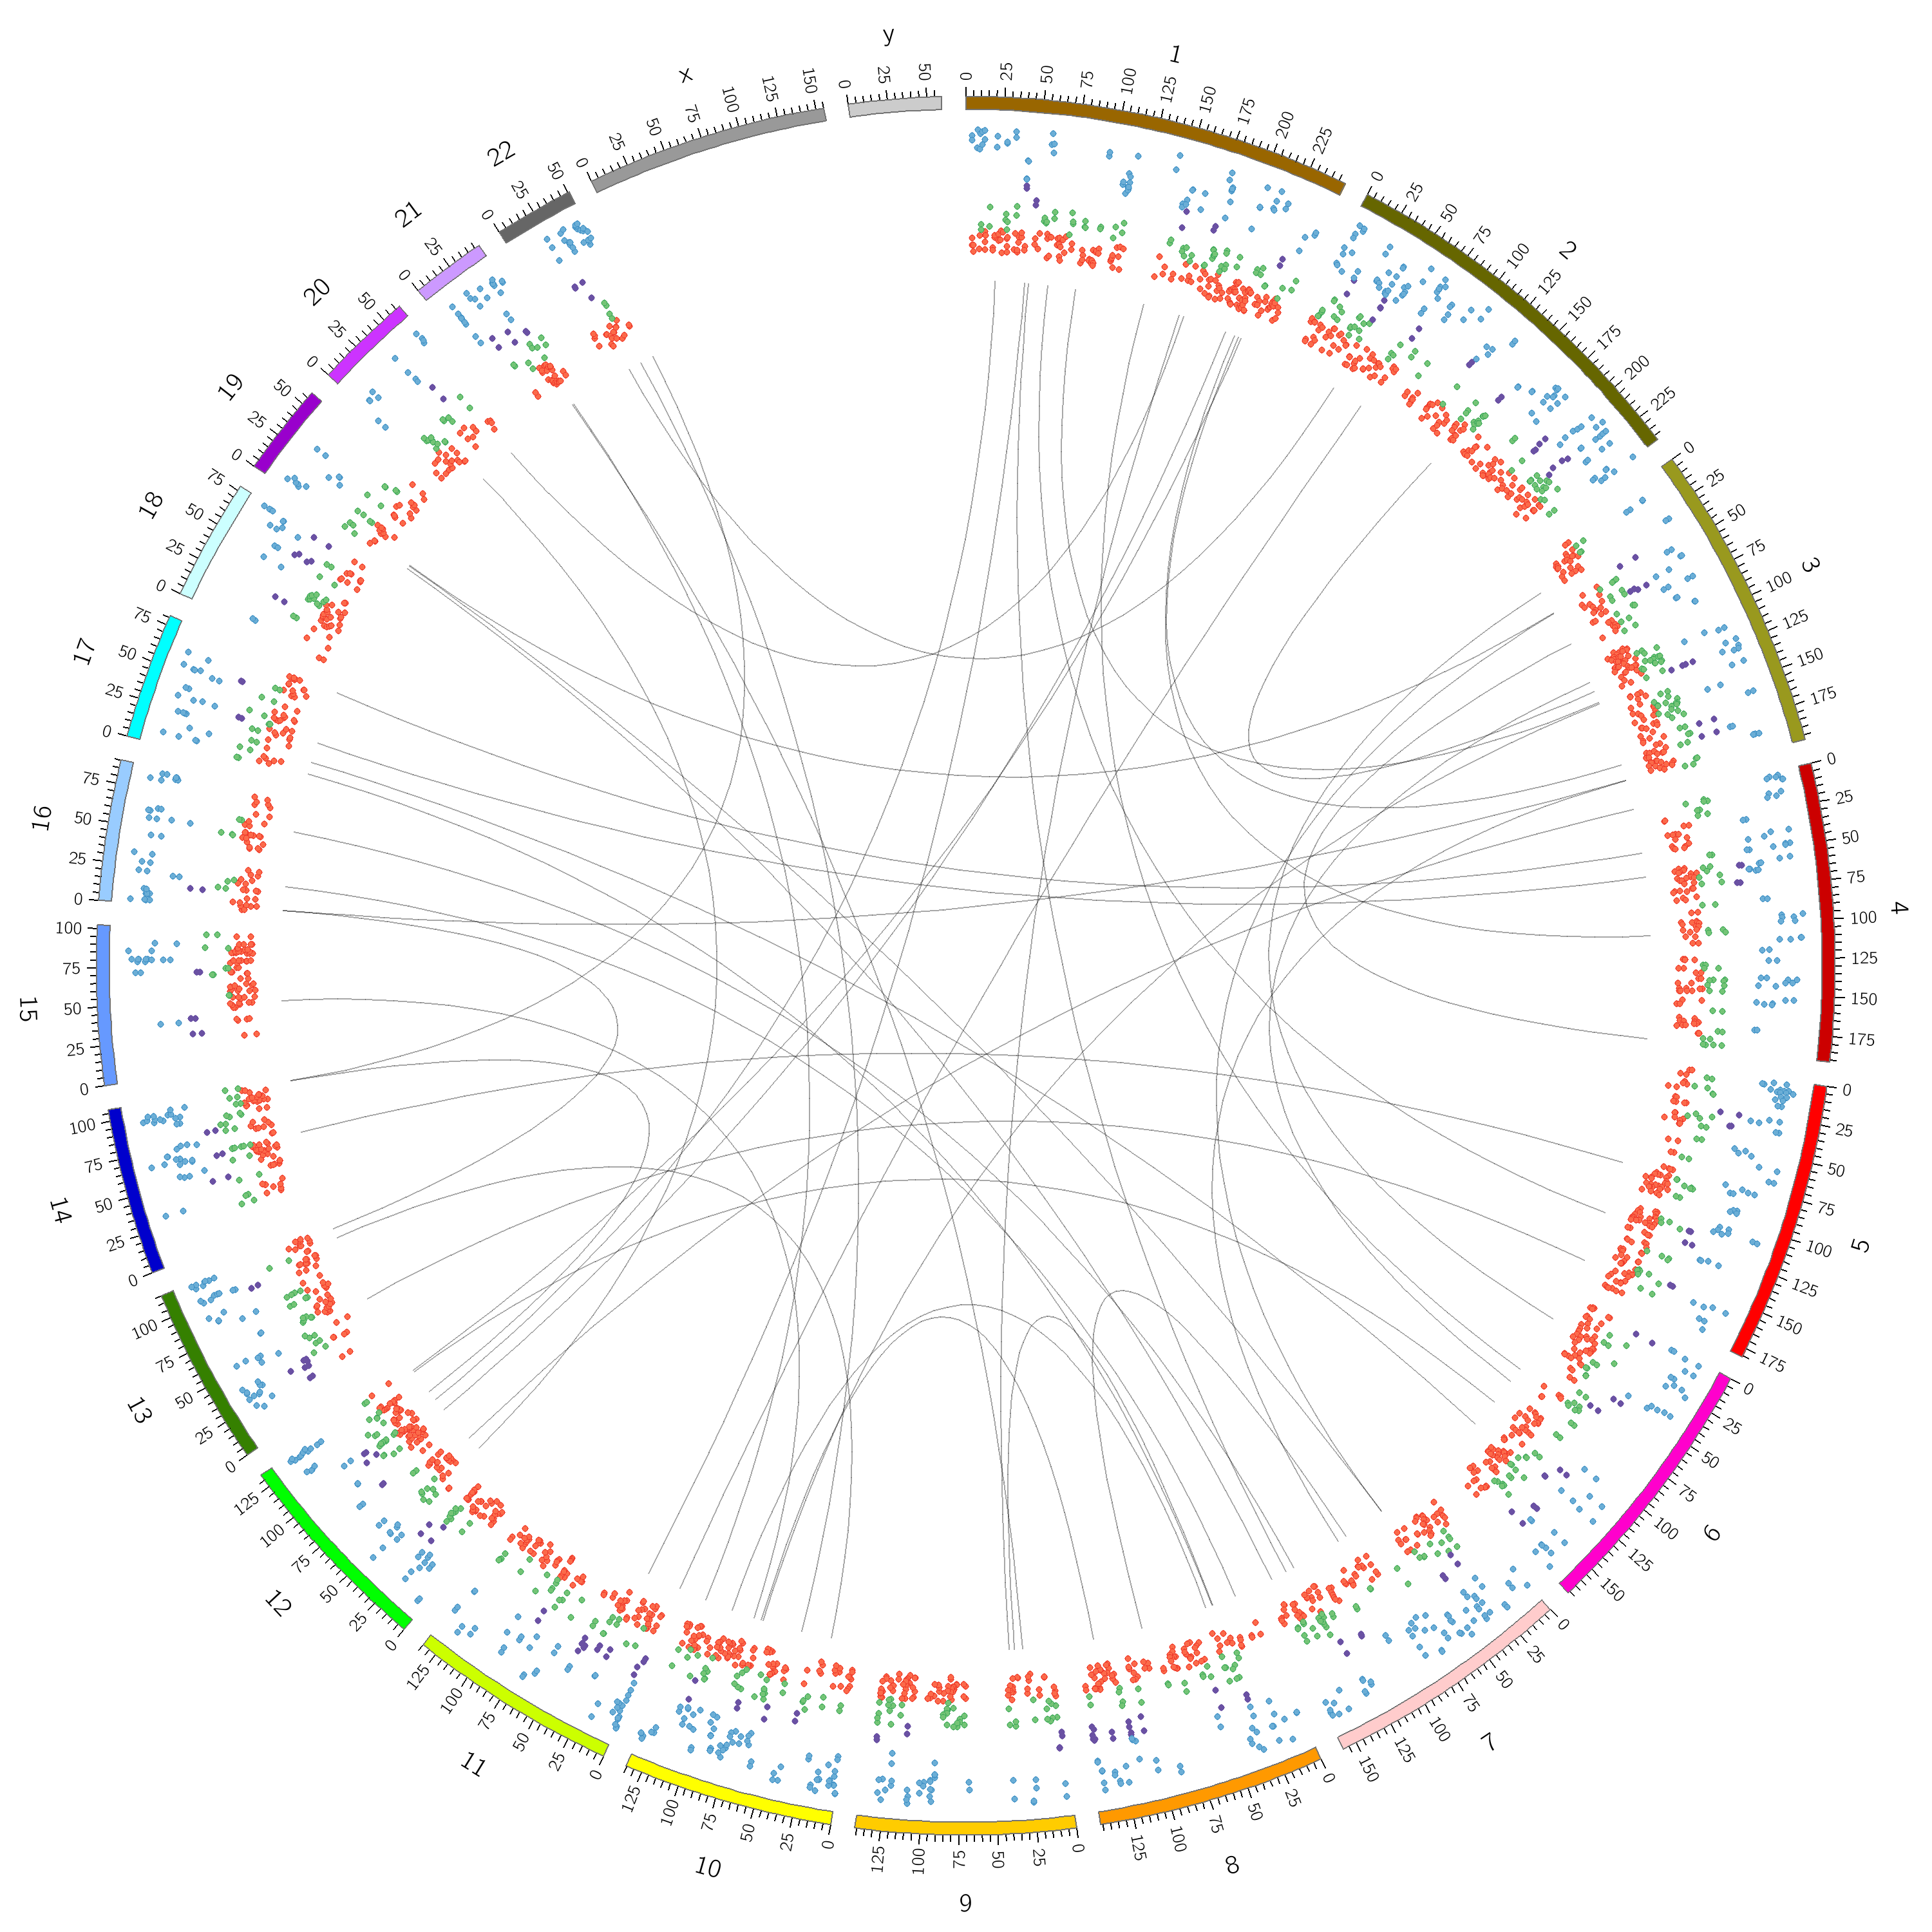
\includegraphics[keepaspectratio,width=0.5\textwidth]{./figures/circos/LX1_0529} \\
eWGA gDNA & eWGA 1 \\
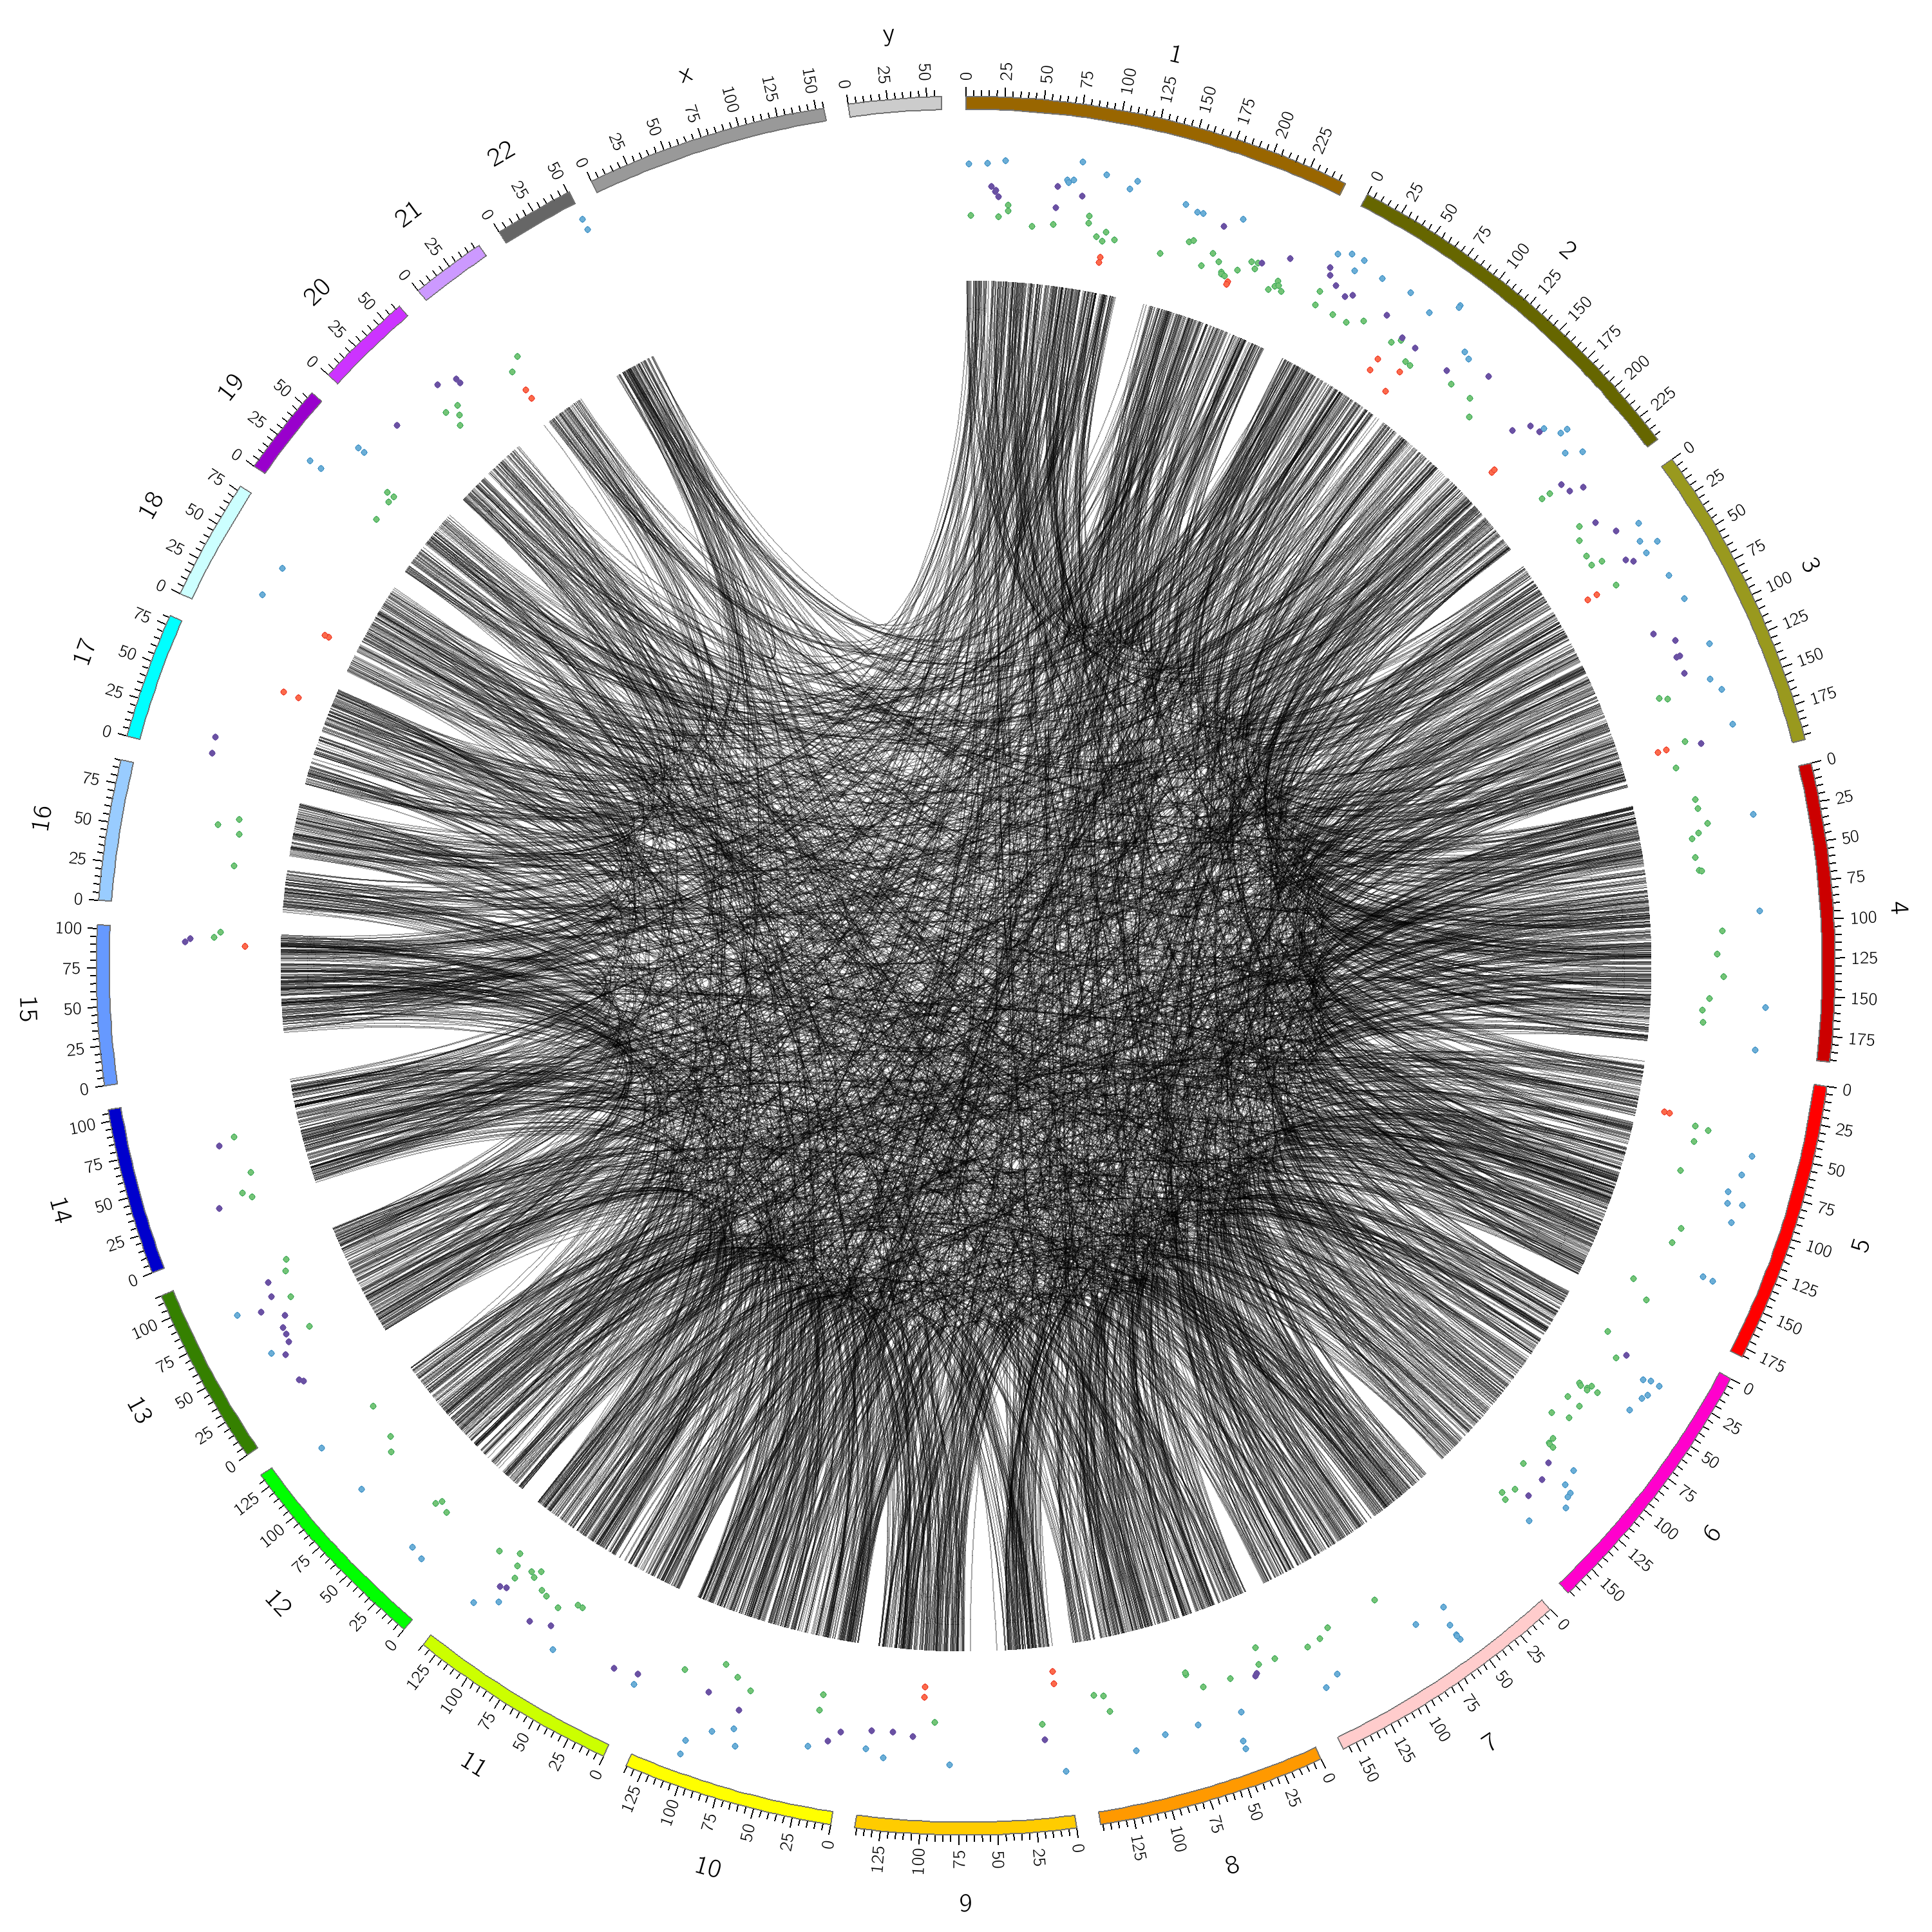
\includegraphics[keepaspectratio,width=0.5\textwidth]{./figures/circos/SRR1777284gDNA_0529} & 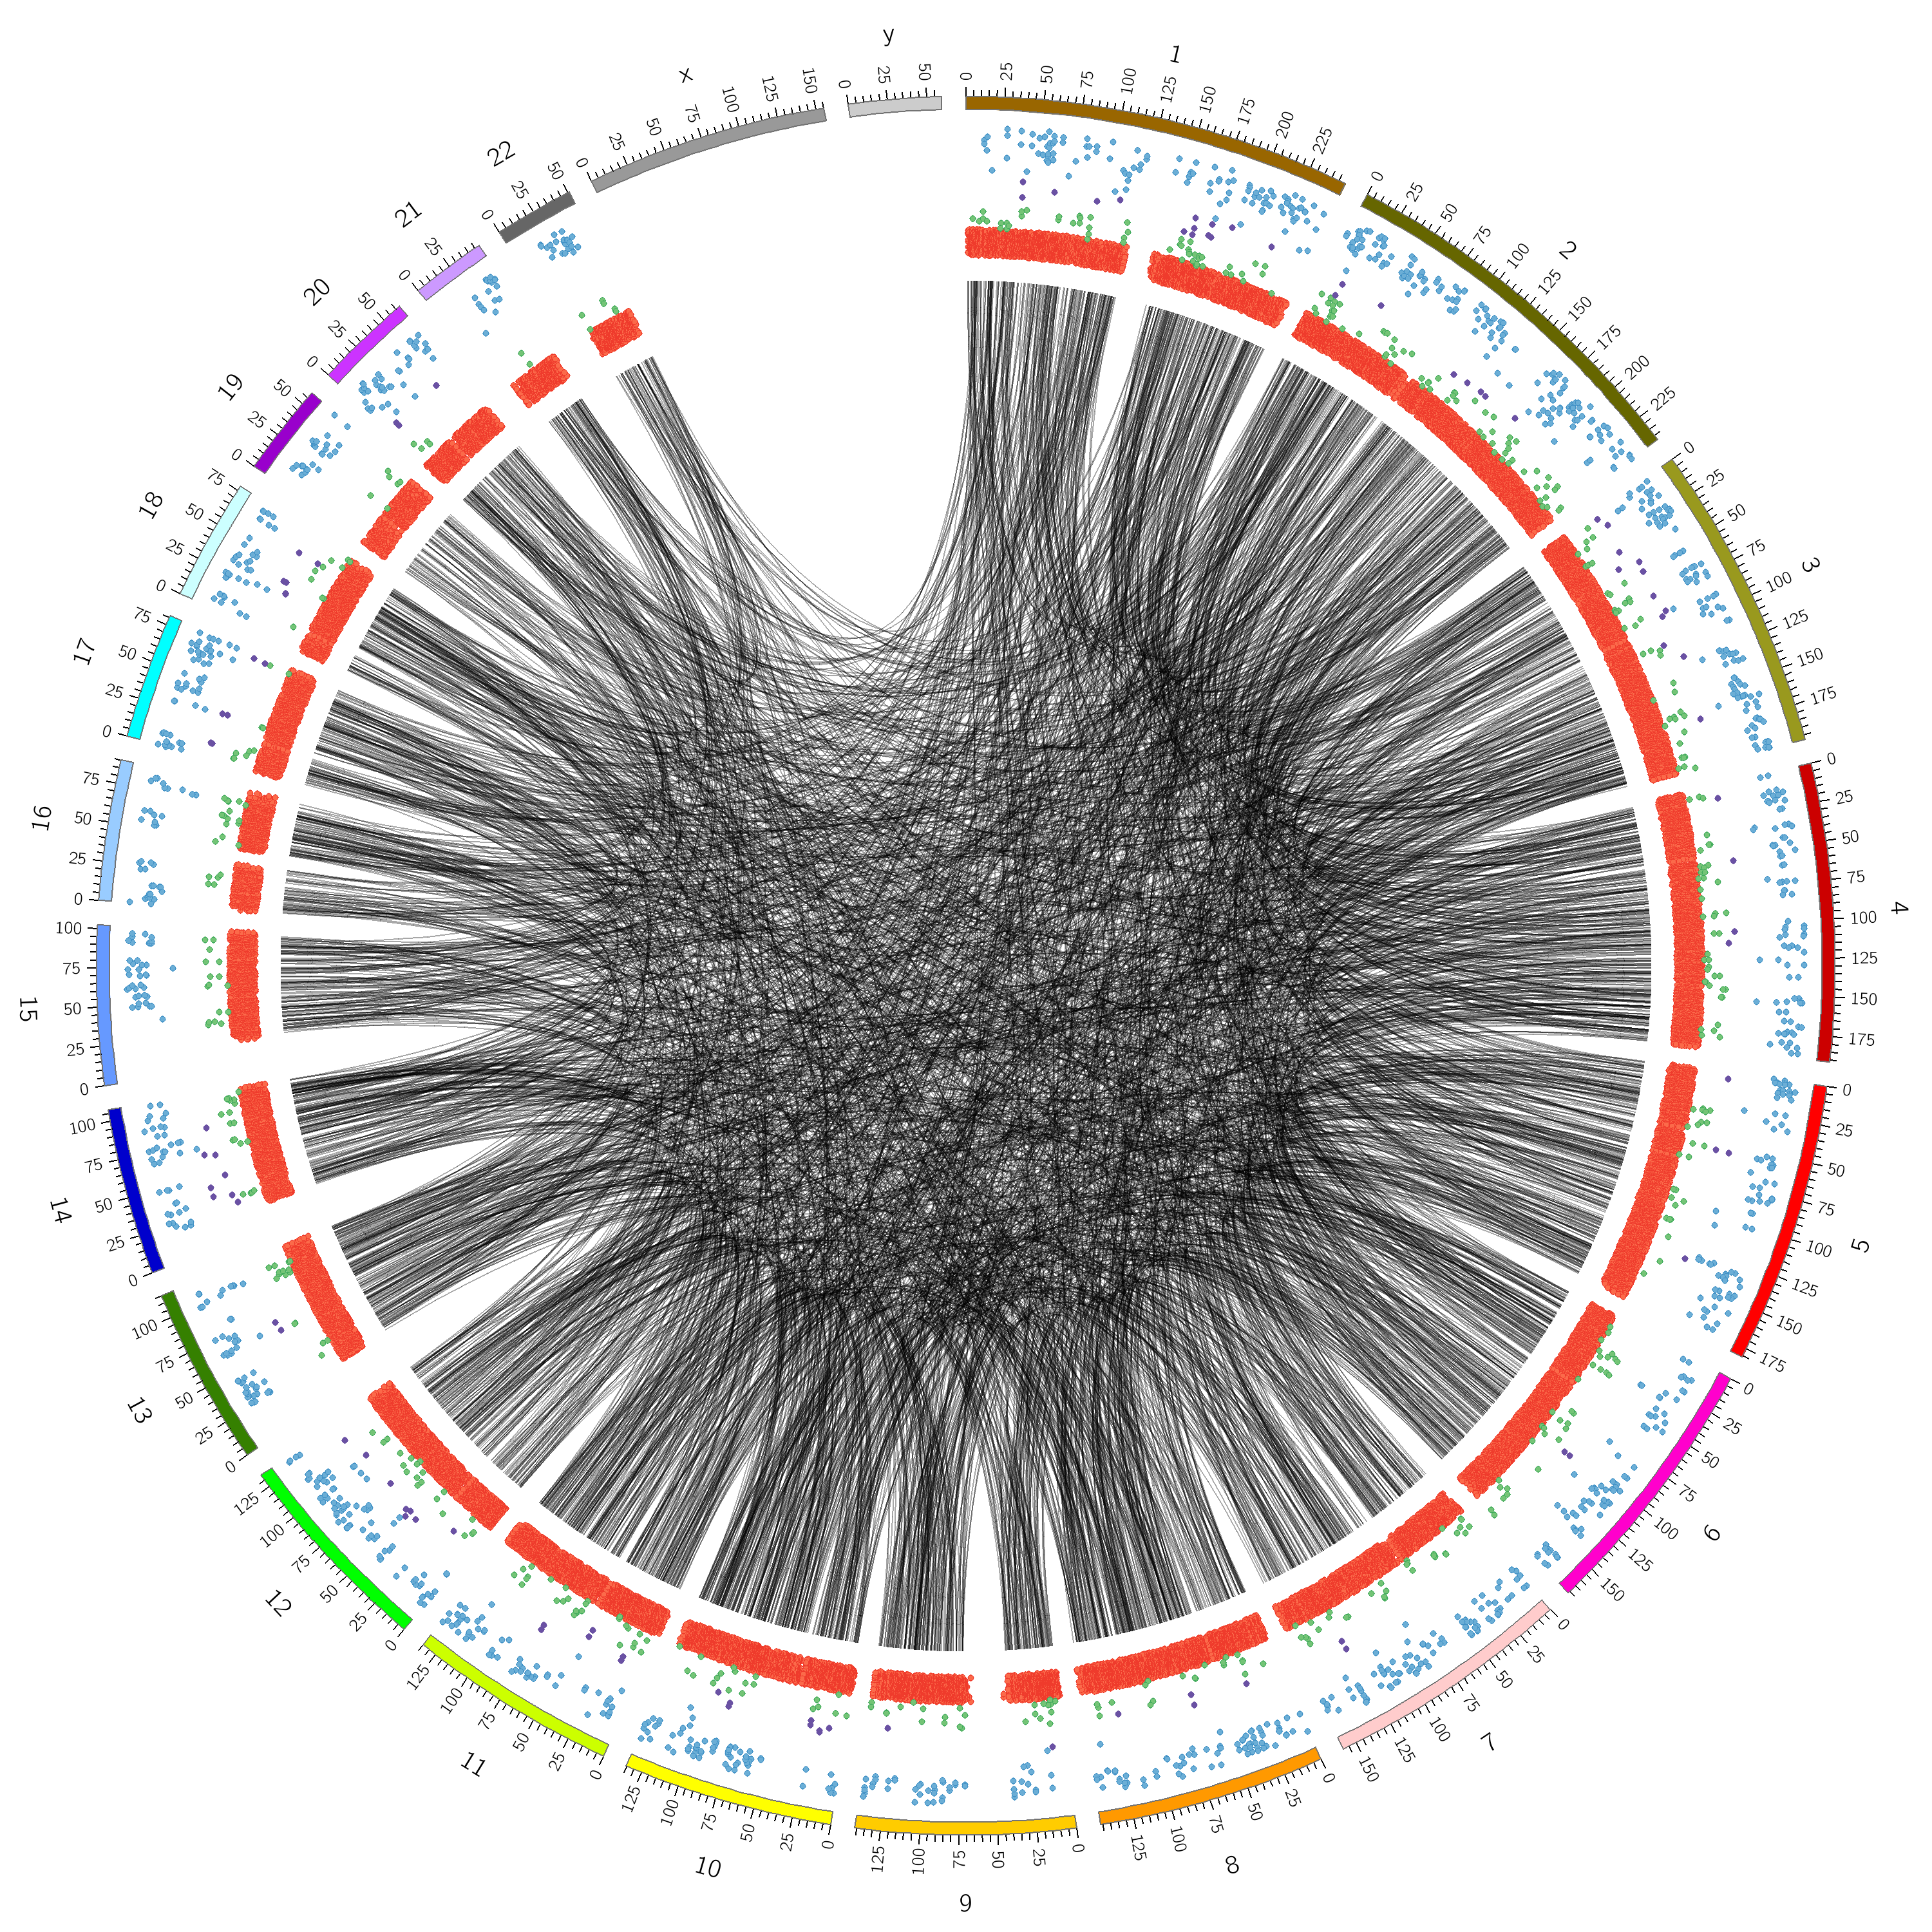
\includegraphics[keepaspectratio,width=0.5\textwidth]{./figures/circos/SRR1777287_0529} \\
\end{tabular}
\caption[Chimera breakpoints shown in Circos plots (part 1)]{Chimera breakpoints shown in Circos plots for bulk genomic DNA and single-cell samples (part 1). Cross-chromosome chimera pairs are connected, shown as black lines in the center. Inverted chimera breakpoints are represented as red dots. Inverted \& large-insert chimera breakpoints are green dots. Large-insert chimera breakpoints are purple dots. Outward chimera breakpoints are blue dots.}
\label{fig:LX0gDNAcircos}
\end{figure}

\begin{figure}
\begin{tabular}{cc}
Nanodrop gDNA & Nanodrop 1 \\
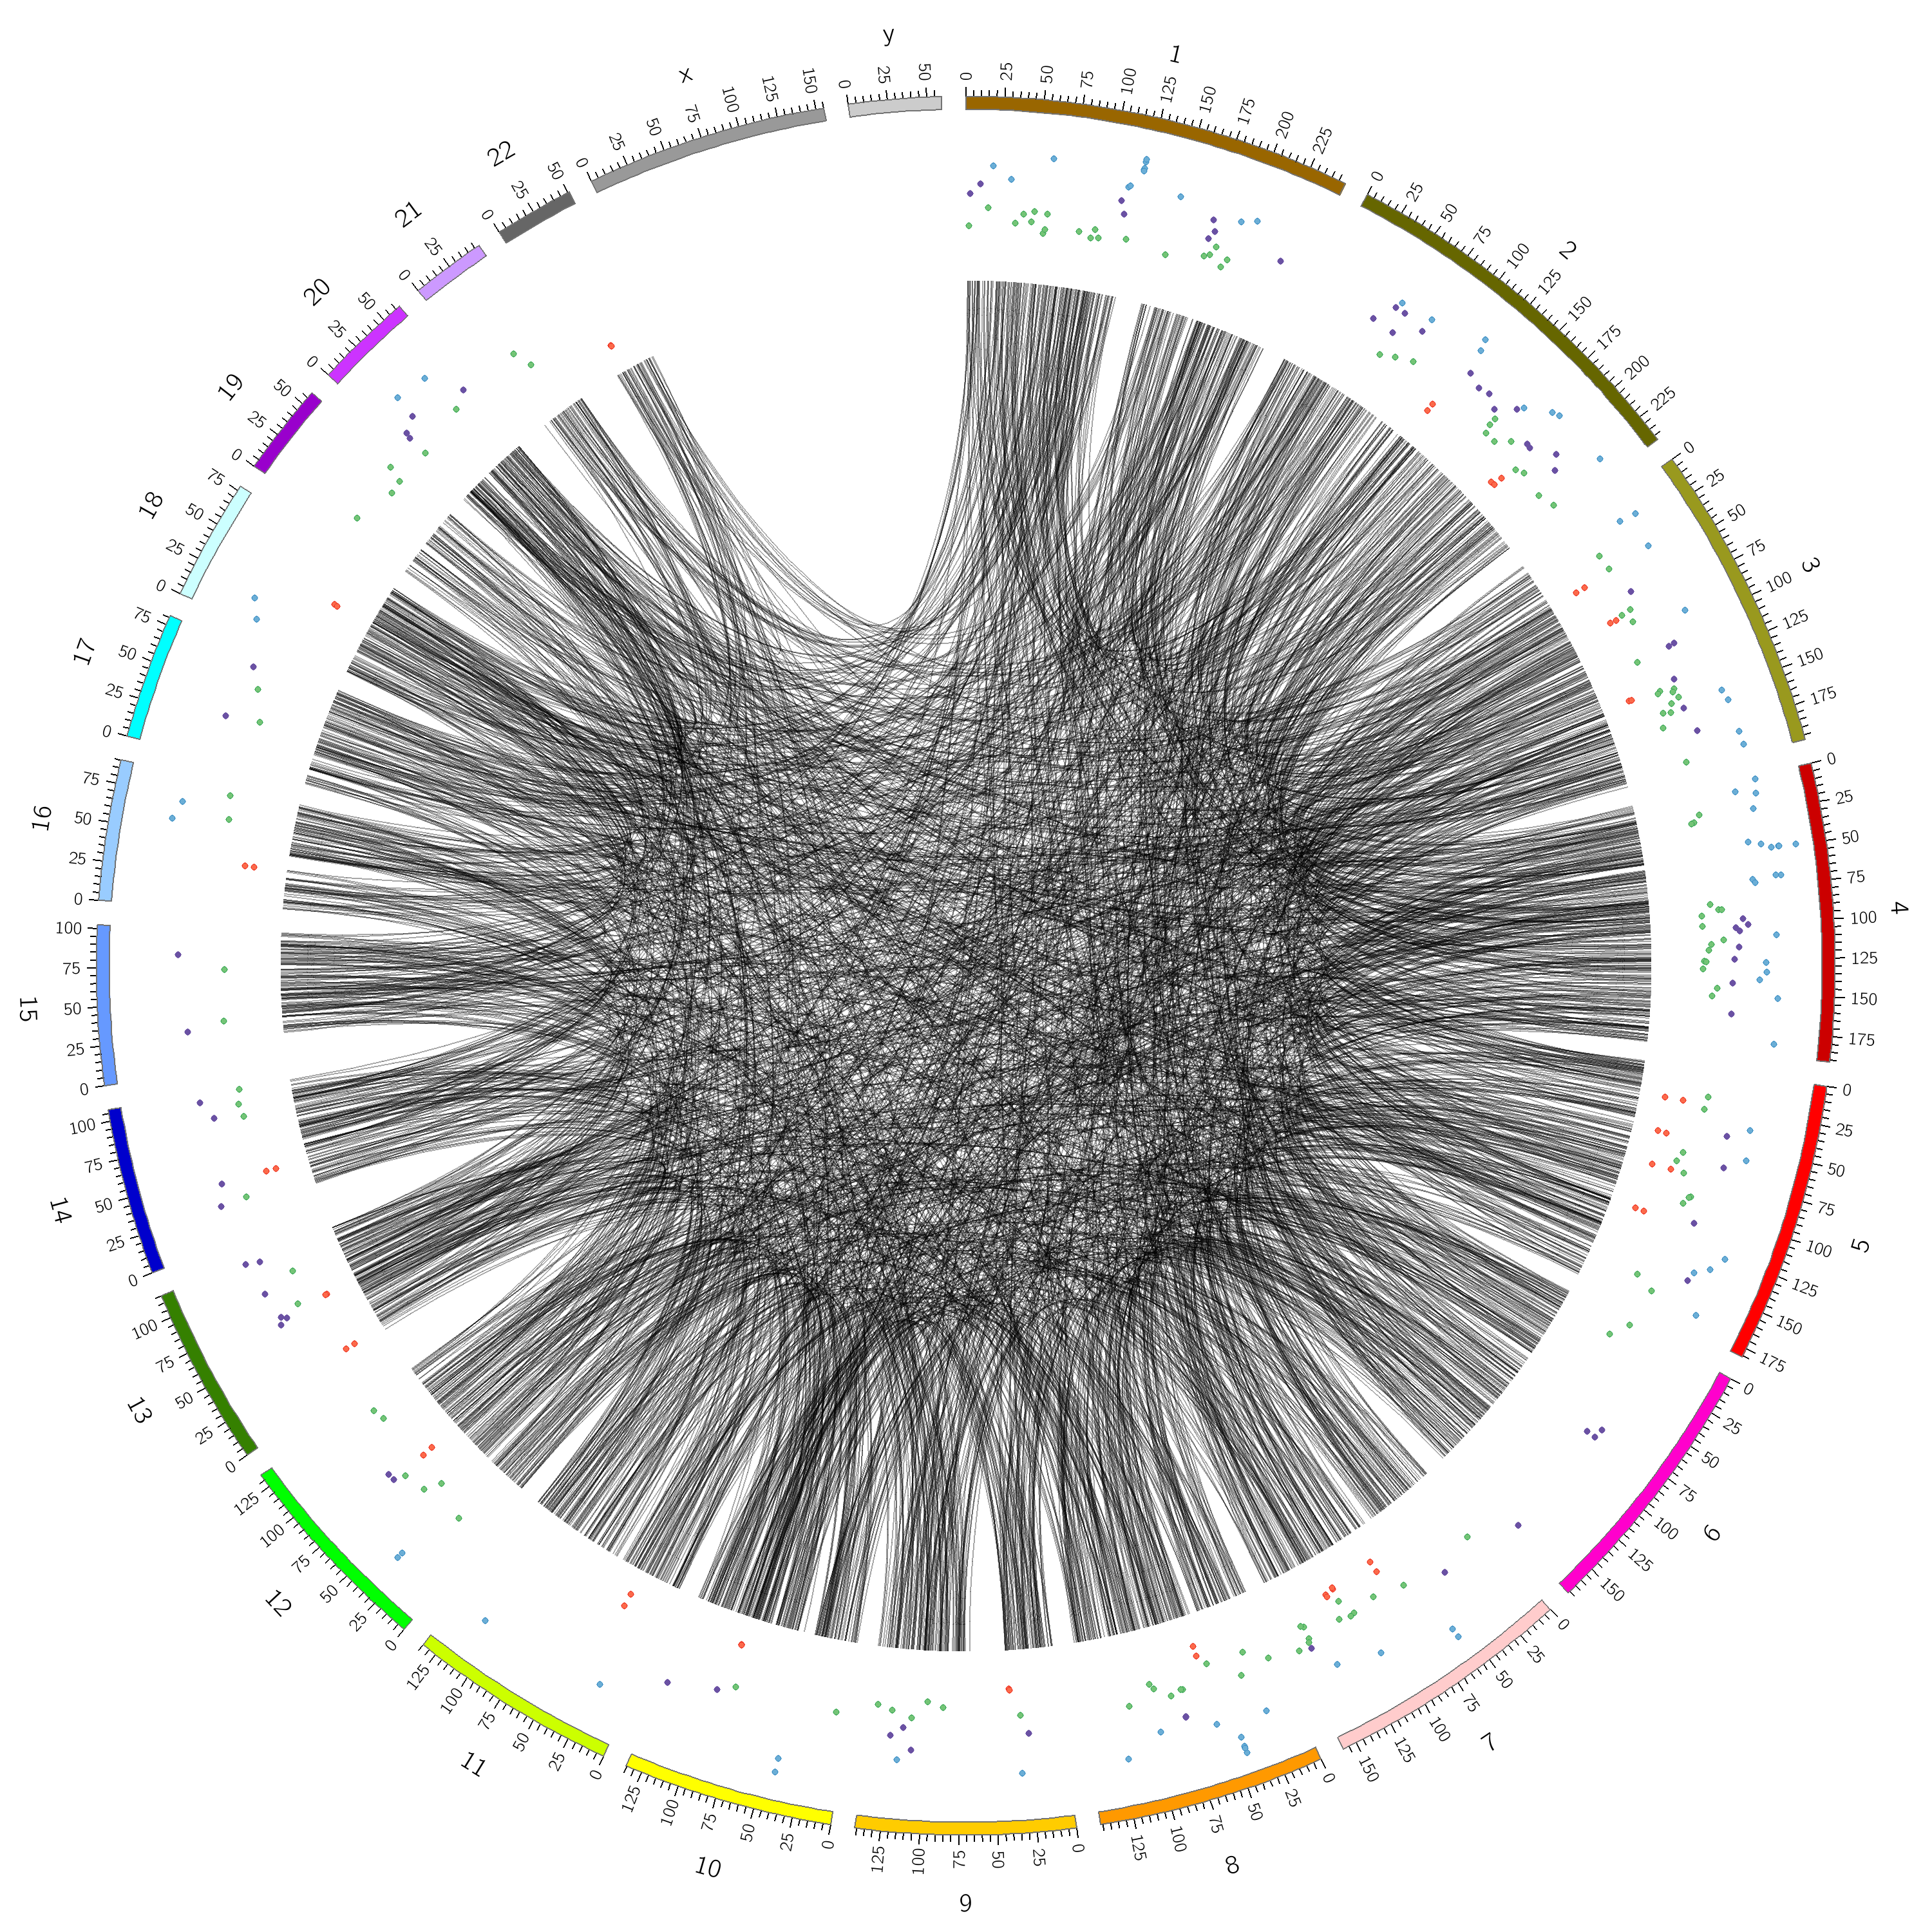
\includegraphics[keepaspectratio,width=0.5\textwidth]{./figures/circos/SRR3749000gDNA_0529} & 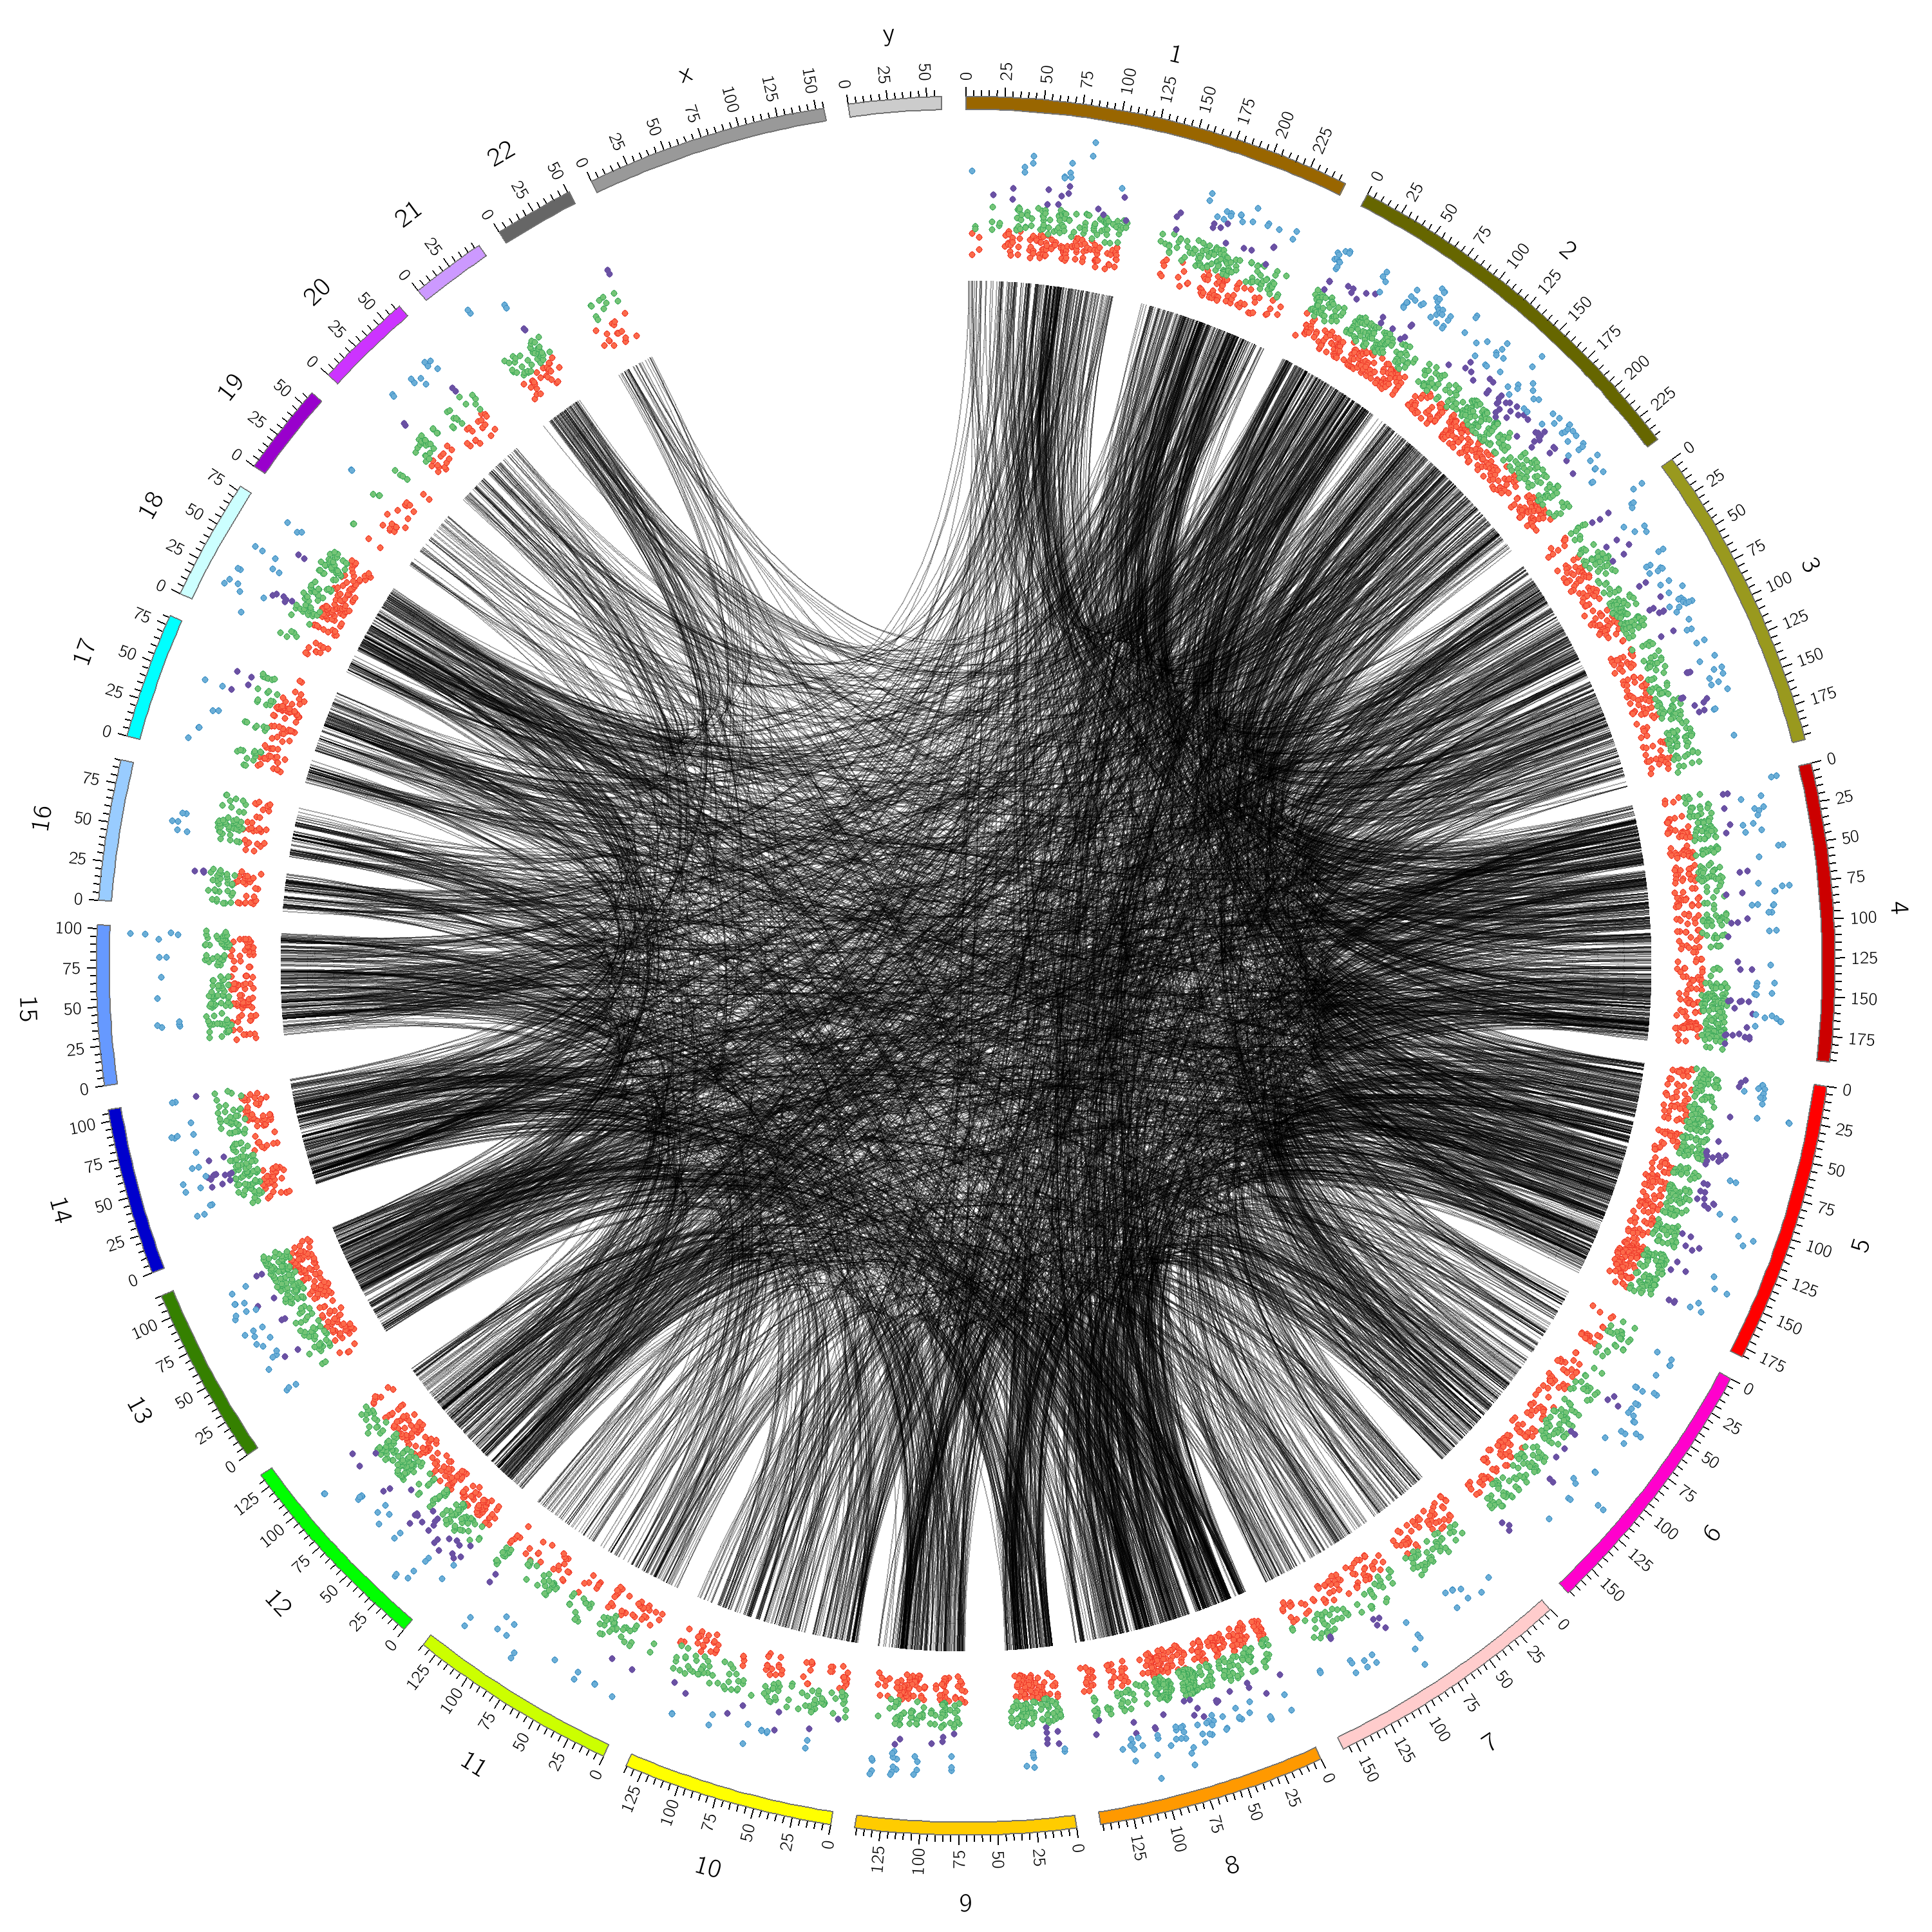
\includegraphics[keepaspectratio,width=0.5\textwidth]{./figures/circos/SRR3749174_0529} \\
LIANTI gDNA & LIANTI 1 \\
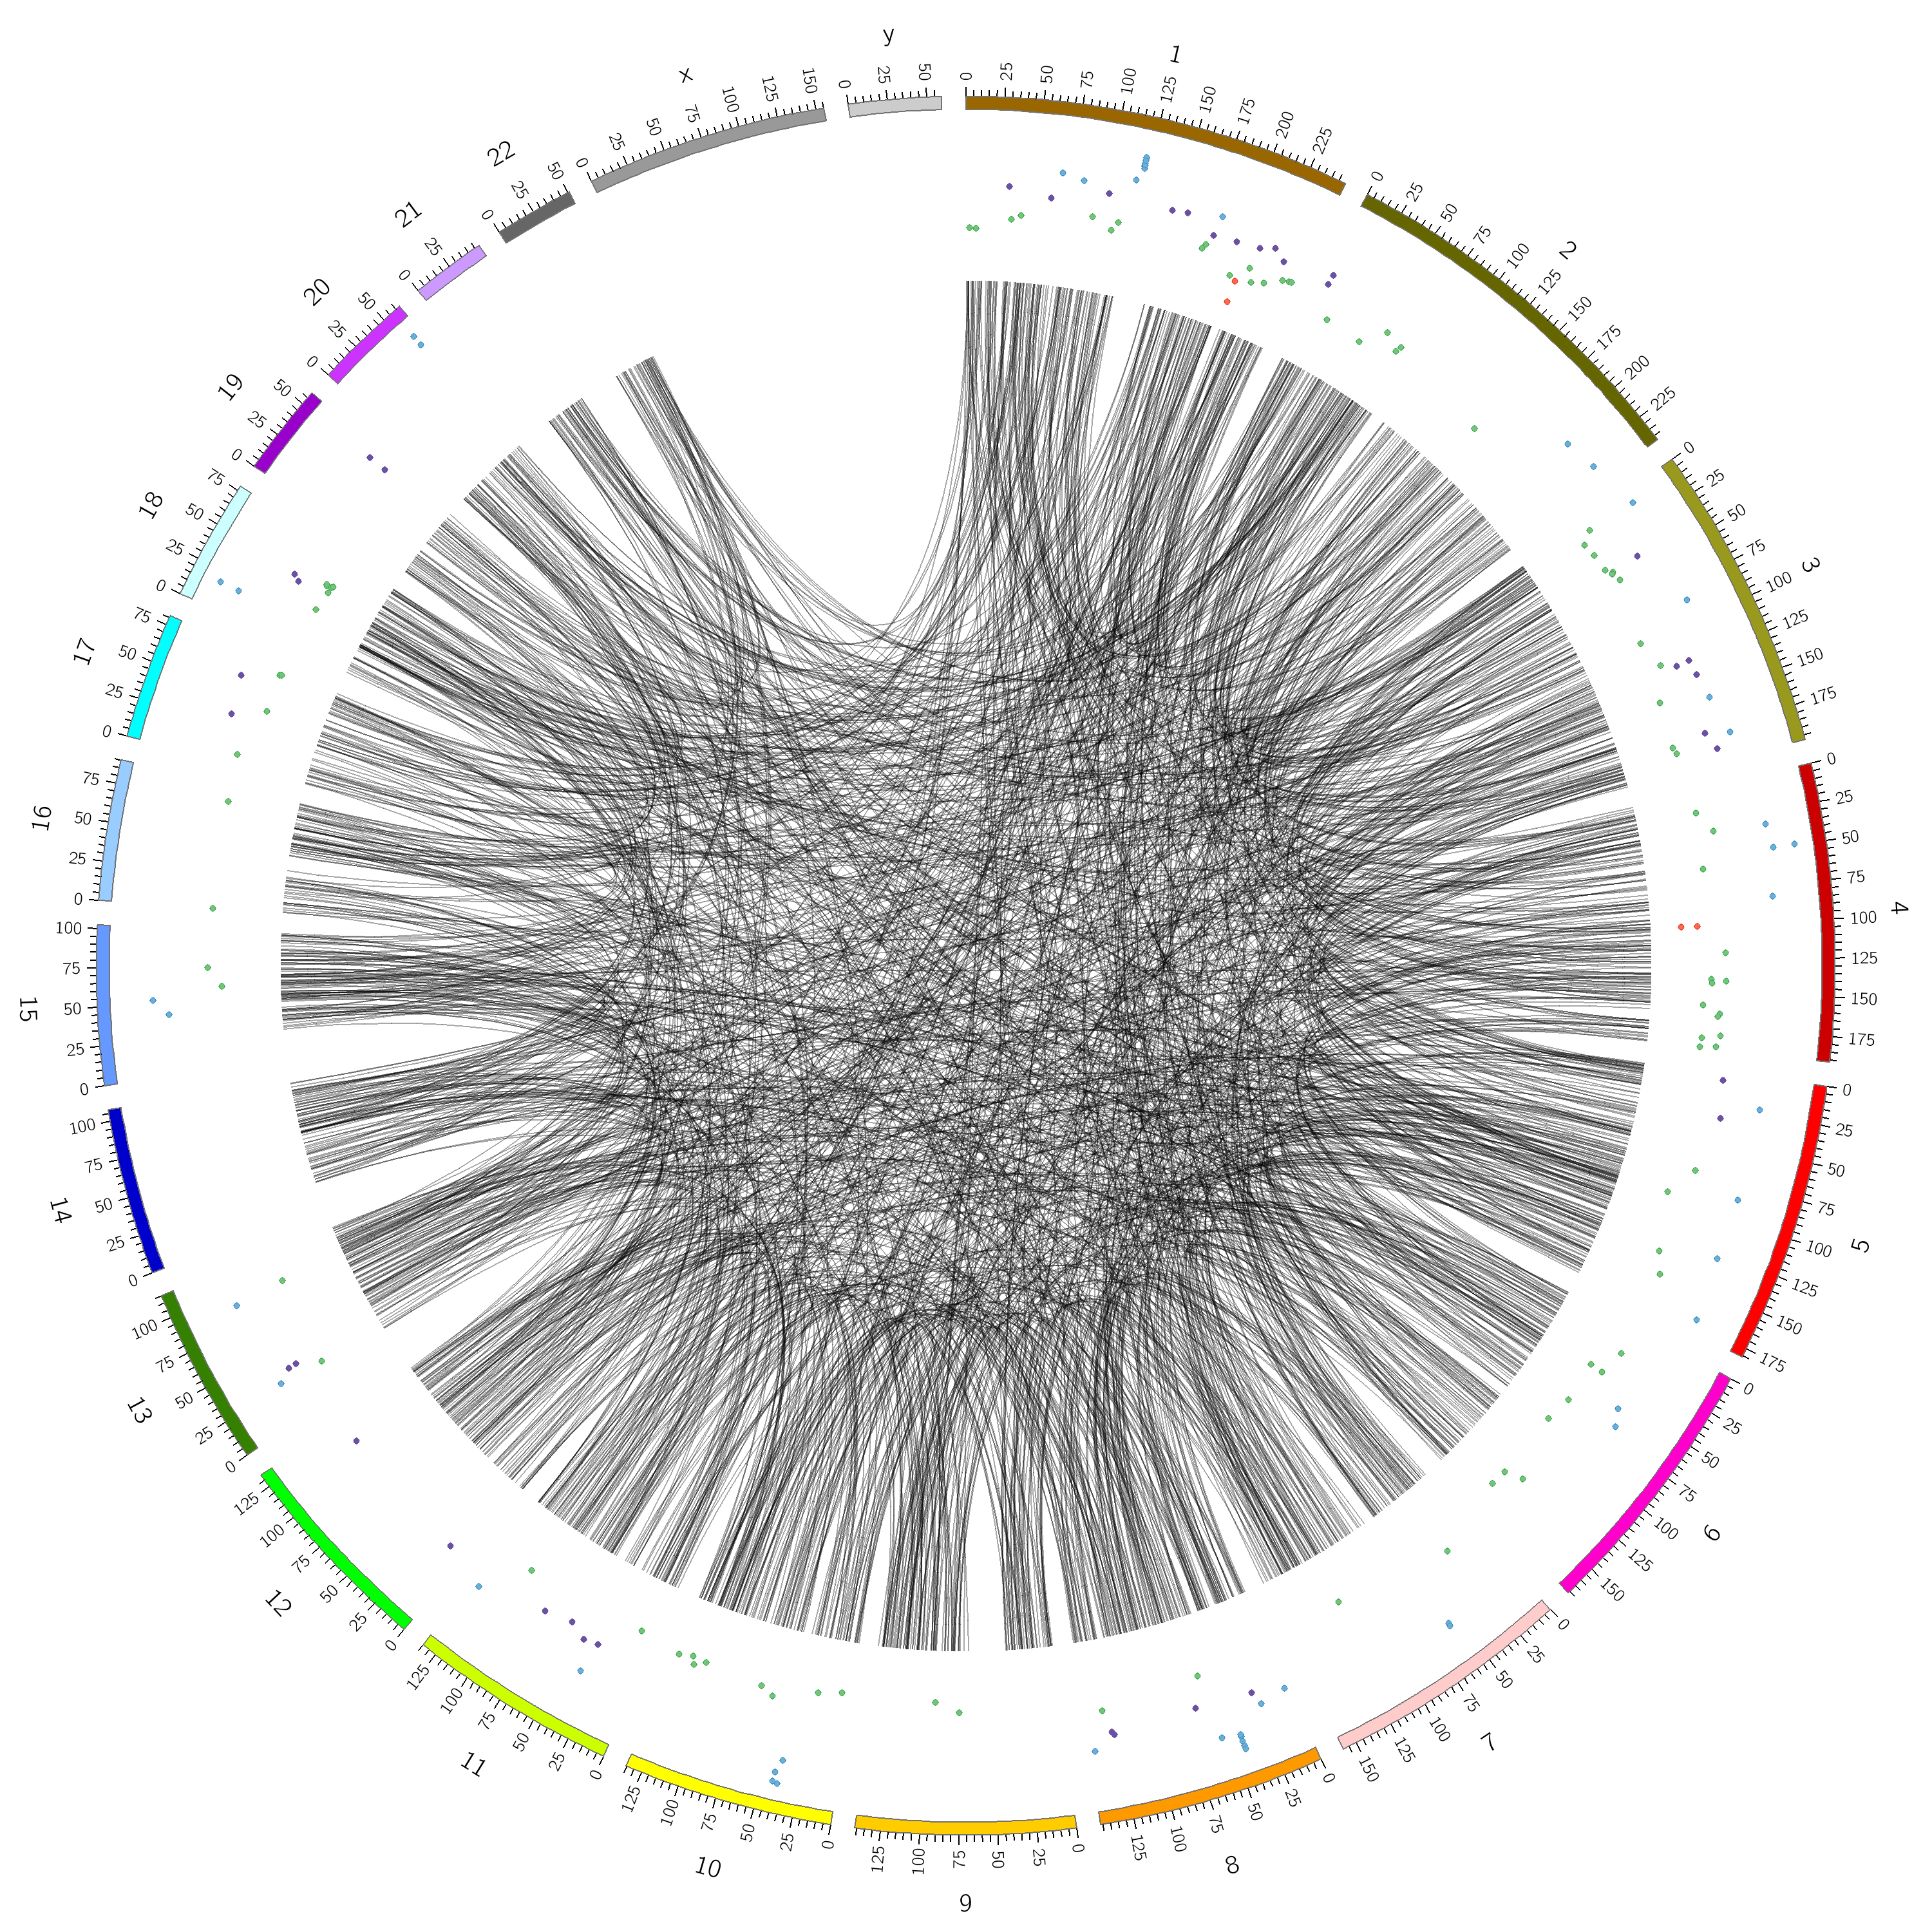
\includegraphics[keepaspectratio,width=0.5\textwidth]{./figures/circos/SRR5365000gDNA_0529} & 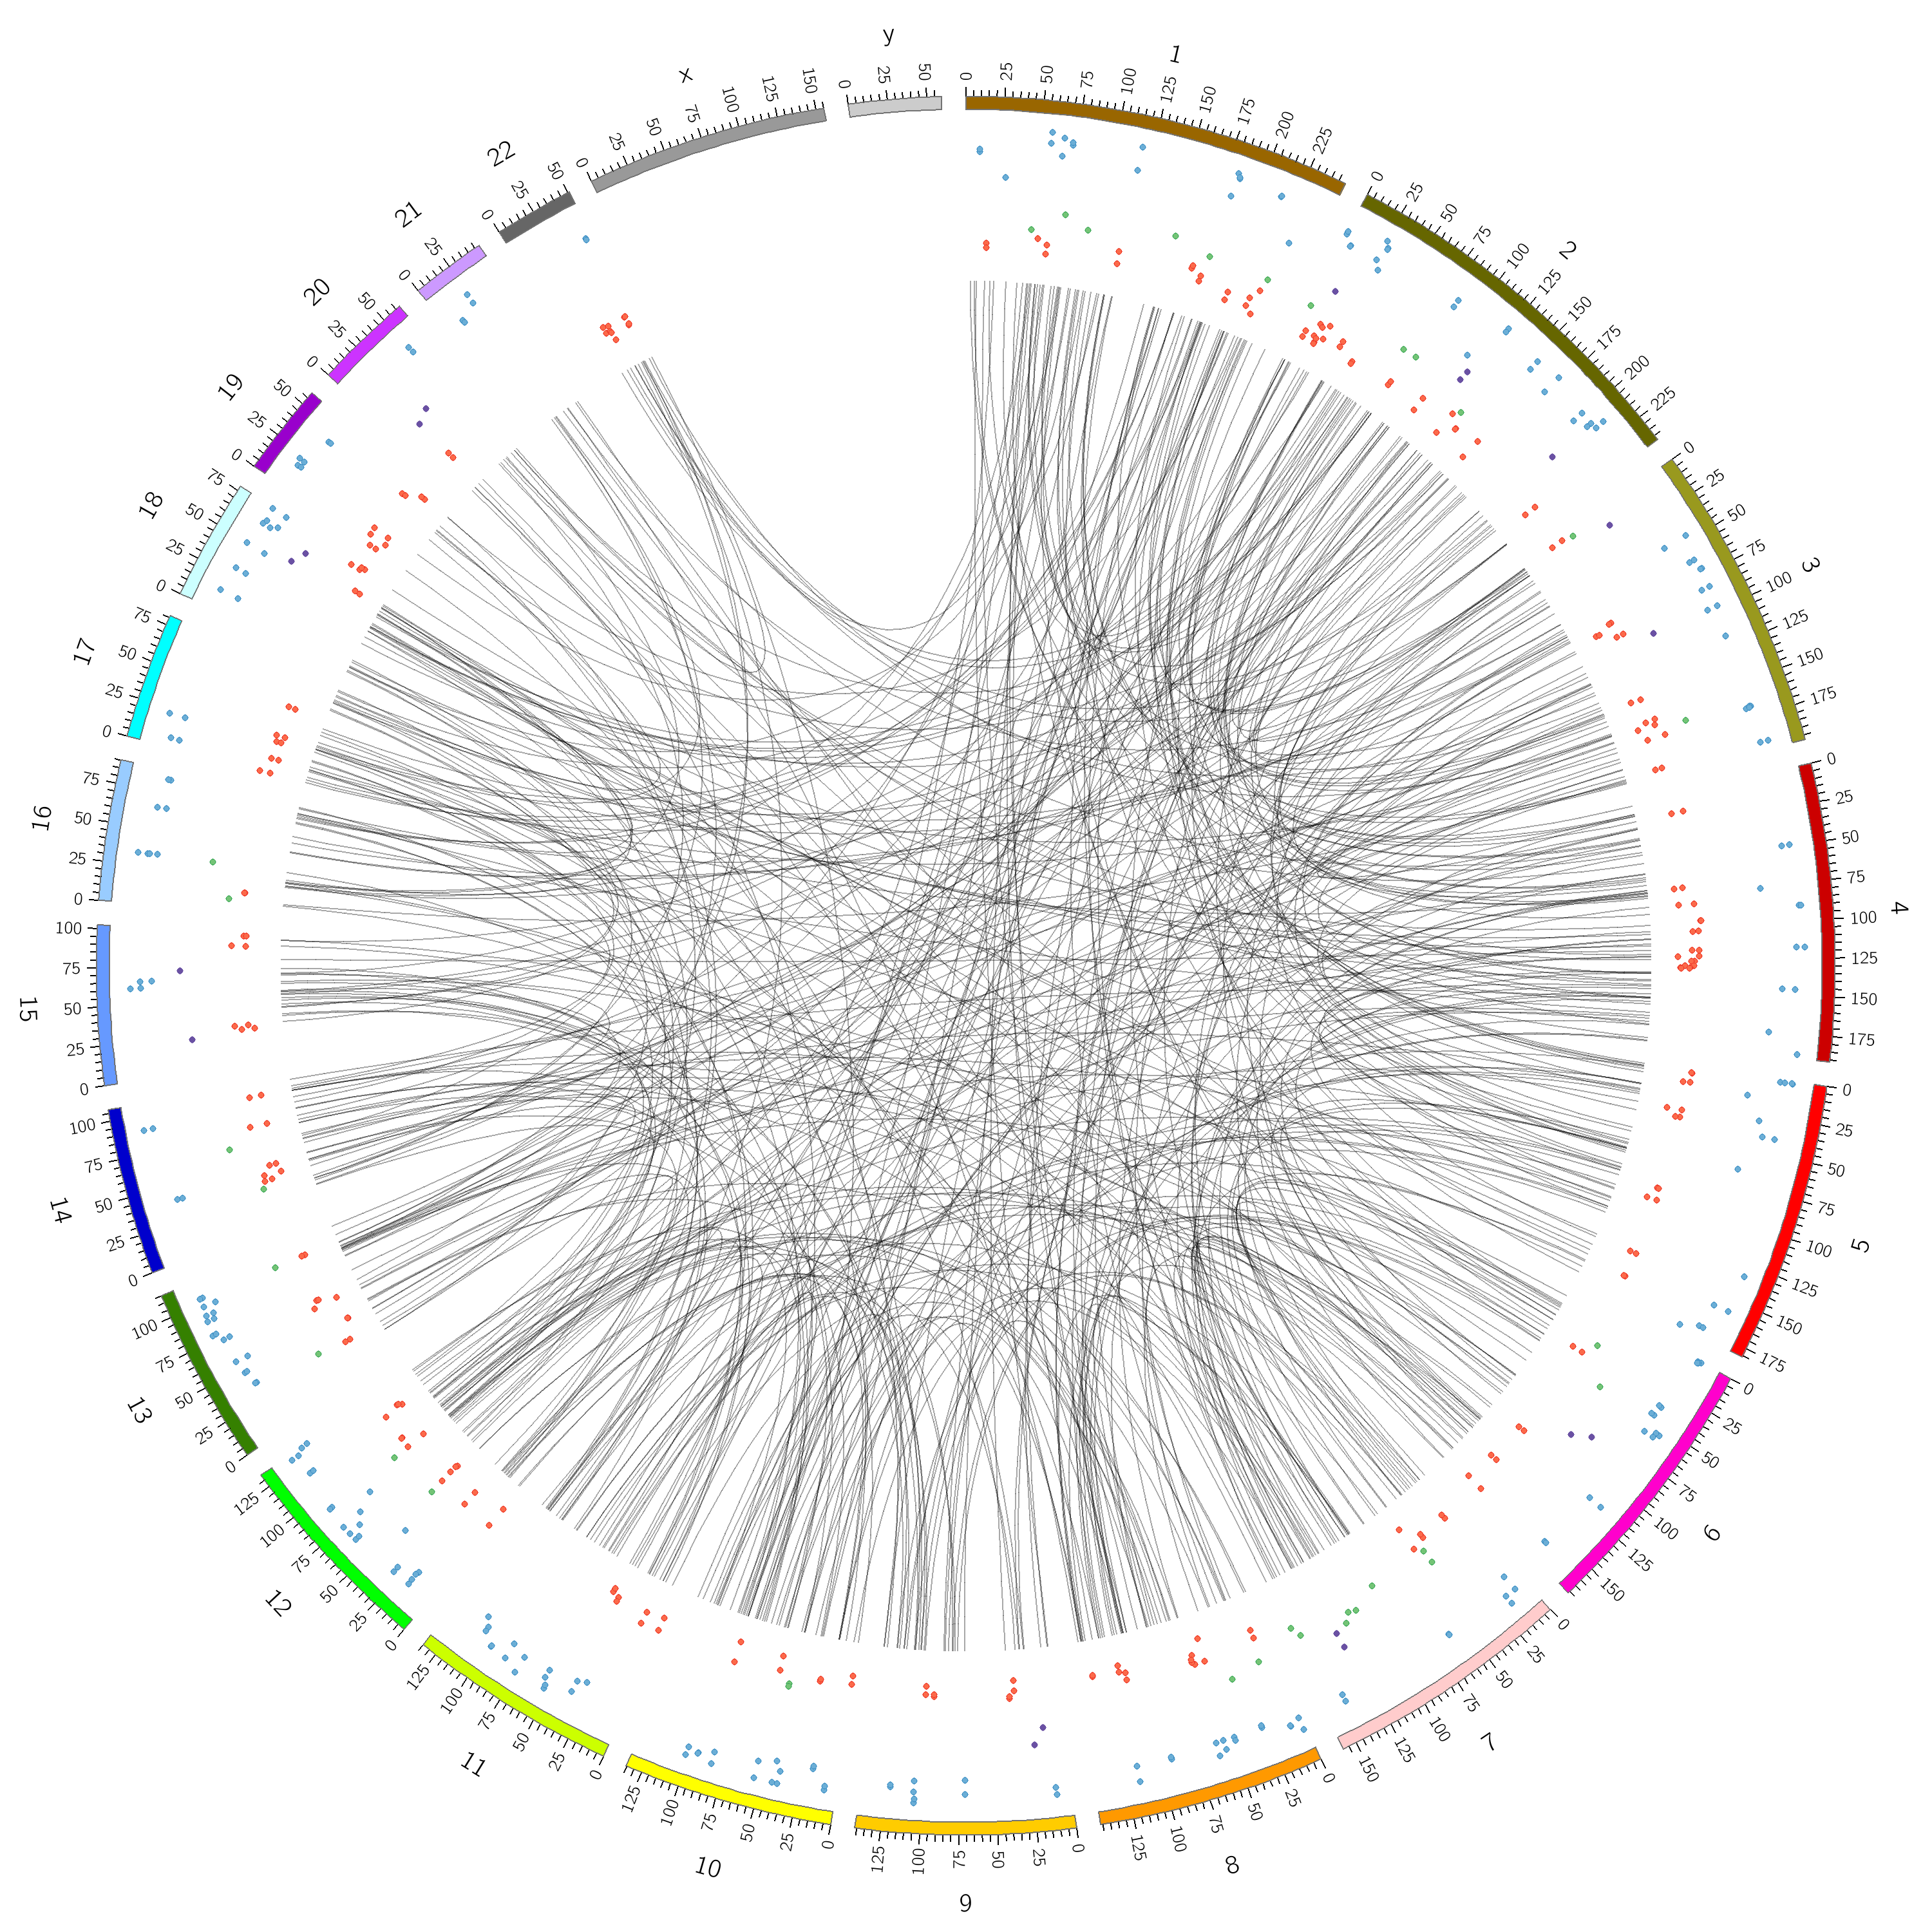
\includegraphics[keepaspectratio,width=0.5\textwidth]{./figures/circos/SRR5365374_0529} \\
\end{tabular}
\caption[Chimera breakpoints shown in Circos plots (part 2)]{Chimera breakpoints shown in Circos plots for bulk genomic DNA and single-cell samples (part 2). Cross-chromosome chimera pairs are connected, shown as black lines in the center. Inverted chimera breakpoints are represented as red dots. Inverted \& large-insert chimera breakpoints are green dots. Large-insert chimera breakpoints are purple dots. Outward chimera breakpoints are blue dots.}
\label{fig:part2_LX0gDNAcircos}
\end{figure}


In order to visualize the location of chimera discovered, I plotted all chimera pairs throughout the genome in Circos plots (Fig. \ref{fig:LX0gDNAcircos} and \ref{fig:part2_LX0gDNAcircos}) \cite{Krzywinski:2009ix}. All chimera pairs shown were based on the normalization of 430K mapped sequencing reads for each sample. Each Circos plot shows the chimera locations across the entire set of chromosomes. The VM gDNA represents the RPE bulk genomic DNA sample without any PCR enrichment, indicating that the unamplified genomic DNA contains a baseline of structural variations with respect to the reference genome. The difference in frequencies of cross-chromosome chimera between the VM gDNA and other gDNA samples probably originate from PCR enrichment and are cell-line specific. This difference shows the difficulty in benchmarking chimera performances across different studies and the importance of standardizing single-cell model systems for future technology development and characterization. 

\begin{figure}
\centering
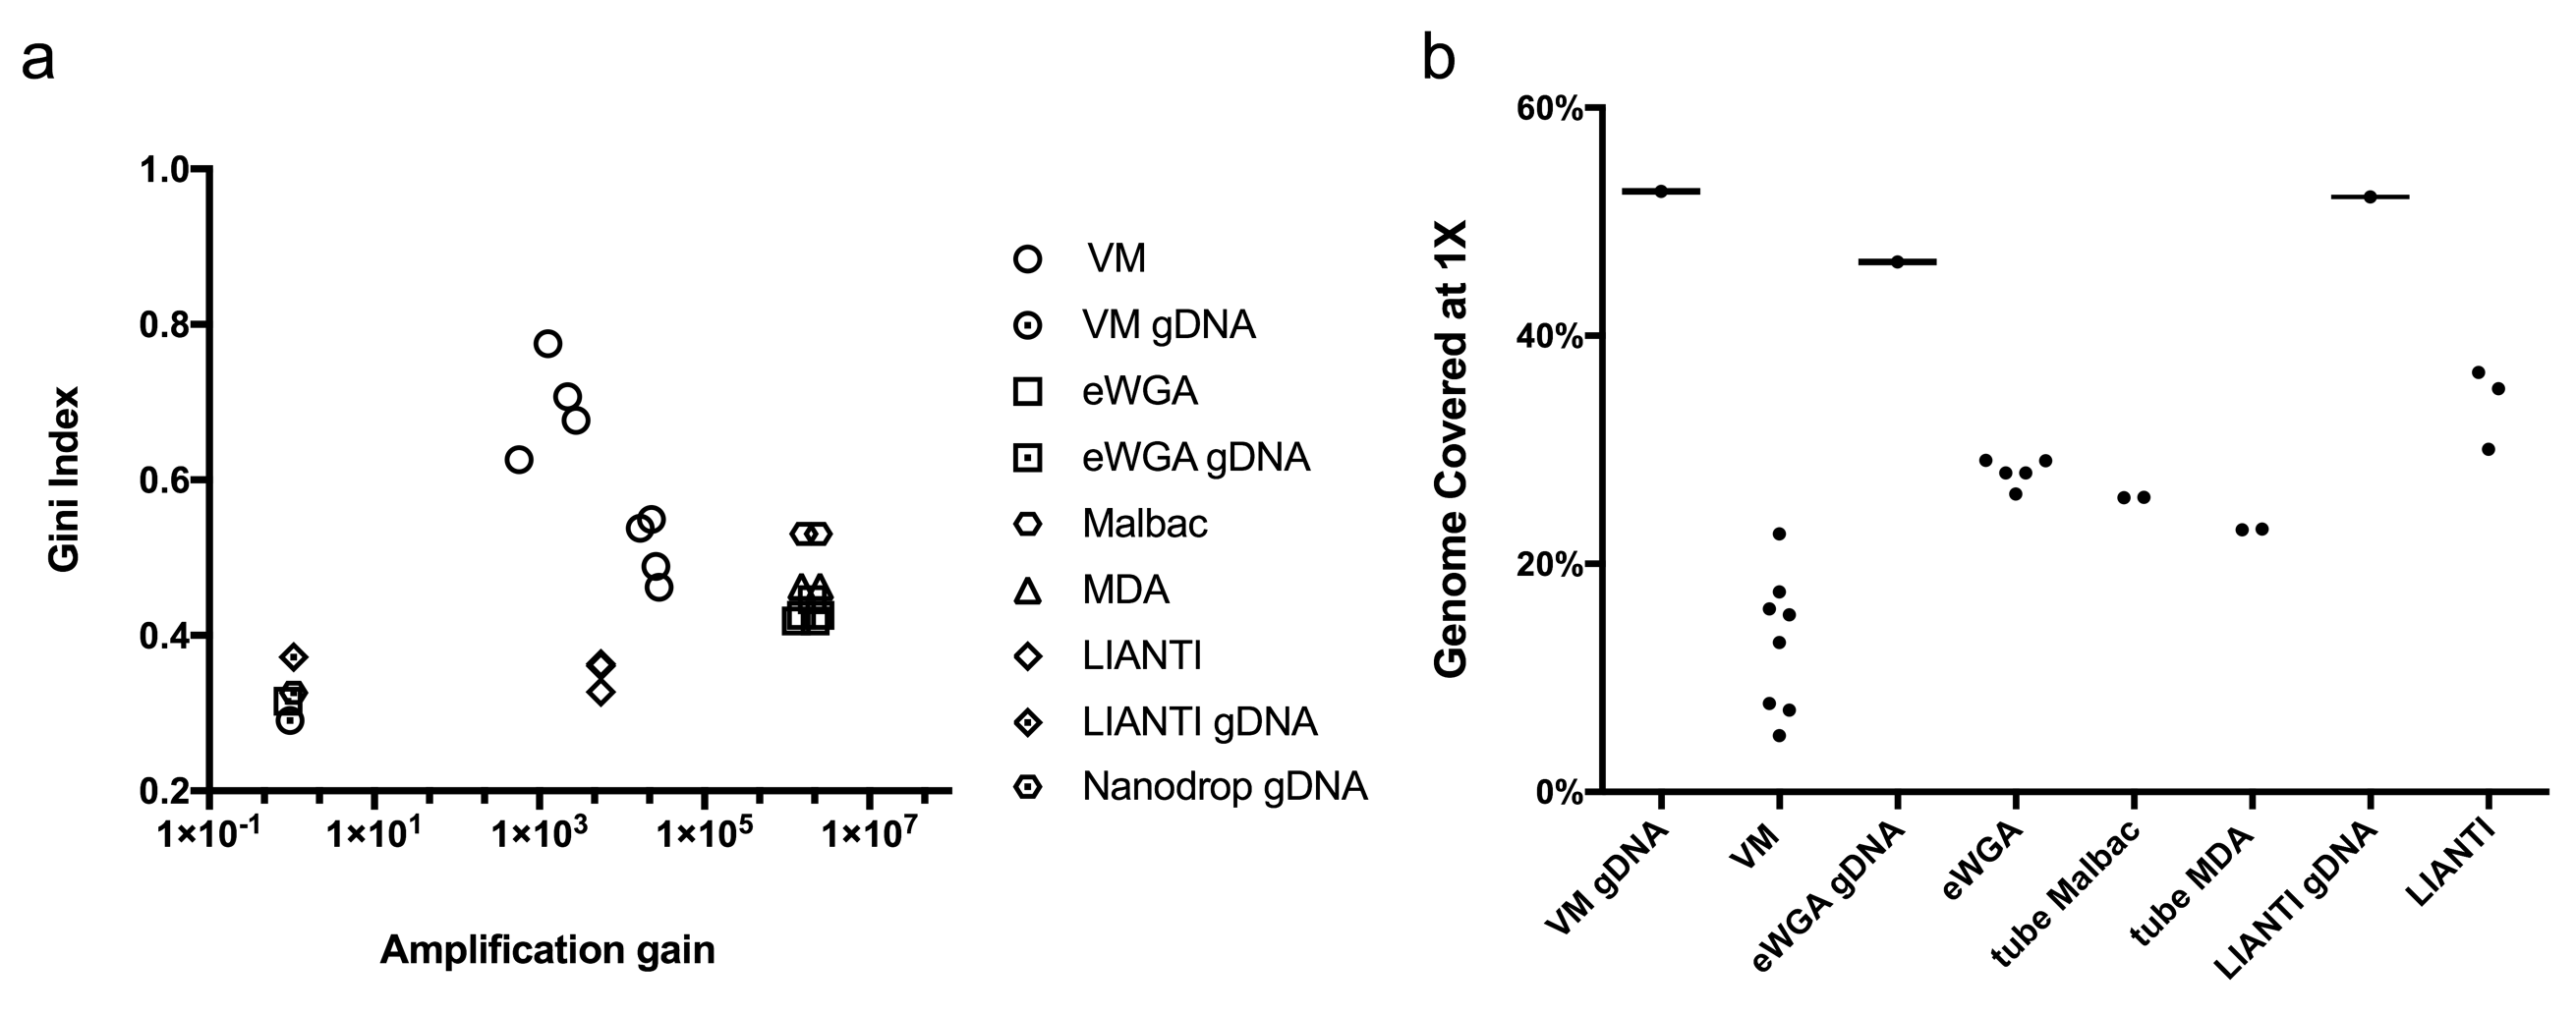
\includegraphics[keepaspectratio,width=1\textwidth]{./figures/GenomecovLorenz}
\caption[The coverage uniformity and the genome coverage performance]{The coverage uniformity and the genome coverage performance. (a) The coverage uniformity is shown as Gini index vs amplification gain. Gini index of 1 means the maximum bias. (b) Genome coverage percentage is shown for all datasets.}
\label{fig:GenomecovLorenz}
\end{figure}

\subsection{Coverage uniformity and physical genome coverage performances}
In order to evaluate the coverage uniformity and the physical genome coverage performance of single amplified human genomes, \textit{virtual microfluidic} VM (8 cells), eWGA (5), MALBAC (2), MDA (2), LIANTI (3) were first downsampled to 1$\times$ mapped depth (about 30 million reads). Fig. \ref{fig:GenomecovLorenz}a quantifies the coverage bias vs amplification gain. The coverage bias is quantified using the area under Lorenz curve and is represented as the Gini index. Including the amplification gain is important for quantifying coverage biases, as the literature has shown MDA over-amplification results in highly biased genomes \cite{deBourcy:2014ji}. Fig. \ref{fig:GenomecovLorenz}b shows the genome coverage percentage across all samples at 1$\times$ mapping depth. \textit{Virtual microfluidic} samples show a range of performance in both coverage uniformity and physical genome coverage percentage. This is most likely due to the uneven amplification gain obtained for 8 different samples (from 28093 to 565 folds). Future experiments with amplification gain control of above 25000 fold should be able to produce much improved overall performance in the coverage uniformity and the genome coverage percentage. Overall, the LIANTI method shows superior performances in terms of coverage uniformity, physical genome coverage and chimera reduction. This new scheme of whole genome amplification might overtake MDA's dominant place in future single cell genomic applications. 

The performances of single-cell analysis are often cherry-picked and selectively reported. The Nanodrop method's high sequencing-depth data were cherry-picked based on the quality of its low-depth dataset, thus we excluded it from the coverage and uniformity comparison. It is highly likely that eWGA and LIANTI single cells are cherry-picked as the best subsets but it is not yet confirmed. The effect of cherry-picking, known as the fallacy of incomplete evidence, gives a false impression on the overall quality of single cell sequencing technologies and inflates performance measurements such as coverage uniformity and genome coverage. In contrast, the 8 VM cells were the entire dataset that went through MDA, library preparation and sequencing (without cherry picking). I believe there is a great potential in improving data qualities and \textit{virtual microfluidics} measurements represent the foremost of single-cell technology platform to this date. 

\section{Conclusion}
In conclusion, \textit{virtual microfluidics} enables high-quality single-cell genome sequencing with 1 (compared with Nanodrop) $\sim$ 8 fold (compared with eWGA) chimera rate reduction in MDA reaction while only requiring basic bench tools. It eliminates the need of creating ultra-small discrete chambers for sub-microliter MDA reactions. This chapter also showcase the importance of quantifying chimeric DNA rearrangements from single-cell genomic amplification and library preparation processes. Such study is important in providing a baseline analysis of the chimera signatures and can be used for predicting the amount of false positive DNA rearrangements that are of interests to prenatal and cancer diagnosis. \textit{Virtual microfluidics} also has a potential as a flexible platform for combining new WGA chemistry such as LIANTI and library preparation methods involving \textit{in situ} tagmentation that will push the throughput and data quality from single-cell WGA to a new level. 

\section{Materials and Methods}
\subsection{Experimental methods}
The hTERT RPE--1 (ATCC) cell line stably expressing GFP-H2B were cultured in 10\% final concentration of fetal bovine serum (FBS) and 0.01 mg\slash ml hygromycin in ATCC-formulated DMEM:F12 Medium (Catalog No. 30--2006). When the culture was at > 80\% confluence, it was serum-starved for 12 hrs overnight for cell cycle synchronization. A blank Costar 384-well plate with glass bottom was imaged for GFP fluorescence and under the white light before cell deposition. Cells were trypsinized, counted and diluted to 1 cell\slash $\mu$l, and 1 $\mu$l was added to each well of the 384 plate. The plate was spin down briefly and imaged for GFP fluorescence and under white light to confirm single-cell occupancy in each well. To the wells with single cells, 4 $\mu$l of lysis buffer (30 mM Tris-HCl, 10 mM NaCl, 5 mM EDTA, 0.5\% Triton X--100 and 1 mg\slash ml proteinase K) with hexamer of final concentration 50 $\mu$M was added and heated at 50 $^{\circ}$C for 3 hrs and at 70 $^{\circ}$C for 30 mins to denature proteinase. Then the plate was heated at 98 $^{\circ}$C for 4 mins and at 95 $^{\circ}$C for 2 mins to ensure proper fragmentation based on eWGA paper. Finally, DNA denaturation happened at 95 $^{\circ}$C for 5 mins, and the plate was cold quenched on ice for 20 mins. 

After cold quenching, PEG hydrogel reaction mix was added to the well. Gels were formed in 20 mins at room temperature and maintain at 30 $^{\circ}$C for 12 hrs for MDA reaction and 65 $^{\circ}$C for 5 mins to deactivate $\Phi$29. Reaction wells were imaged with SYTOX orange DNA intercalating dye. To retrieve DNA for library preparation, 6.6 $\mu$l of 400 mM KOH was added to incubate for 10 mins at 72 $^{\circ}$C and 3 $\mu$l 3.75\% acetic acid neutralization buffer was added. The neutralized gel-DNA mix was SPRI cleaned with 1X:1X volume ratio and library prepared with standard Nextera procedures with 12 cycles of PCR. The 8 cell libraries were loaded on HiSeq 2500 in the rapid run mode. 

The experimental difference from \textit{virtual microfluidics} on the microbial sample is that we diluted single cells and Poisson loaded them into 384 wells. A single genome was fragmented, evenly distributed in the PEG hydrogel and went through digital MDA. Only one round of MDA was conducted. 

\subsection{Bioinformatic methods}

Raw sequencing fastq.gz files were quality and adapter trimmed using Trimmomatic. For fast processing of chimera analysis, fastq files were downsampled to 600,000 reads using Seqtk (https:\slash \slash github.com\slash lh3\slash seqtk with seed 100). Fastq files were mapped with BWA under default mode both pair-ended and single-ended. BAM files were sorted by mapping coordinates. Mark PCR and optical duplicates, and mask repeat region with the file downloaded from UCSC Genome Browser (assembly:GRCh37\slash hg19, group: Repeats, track: RepeatMasker, output:BED). The mapping statistics were retrieved from BAM files using gaemr get\_simple\_bam\_stats.py, and all BAM files were downsampled based the BAM stats resulting to 430,000 reads each sample ---both forward and reverse reads. Single-ended mapped BAM files were sorted by query names and merged (Fig. \ref{fig:Chimera_Mapping}). 

Genome coverage was obtained using Bedtools genomecov. Lorenz curves were obtained by first processing BAM files (duplicates marked) using SAMtools mpileup and then ranking the ascending coverage per base pair (see Fig. \ref{fig:ESDataAnalysis} in Chapter 3 for detail). 

\begin{figure}
\centering
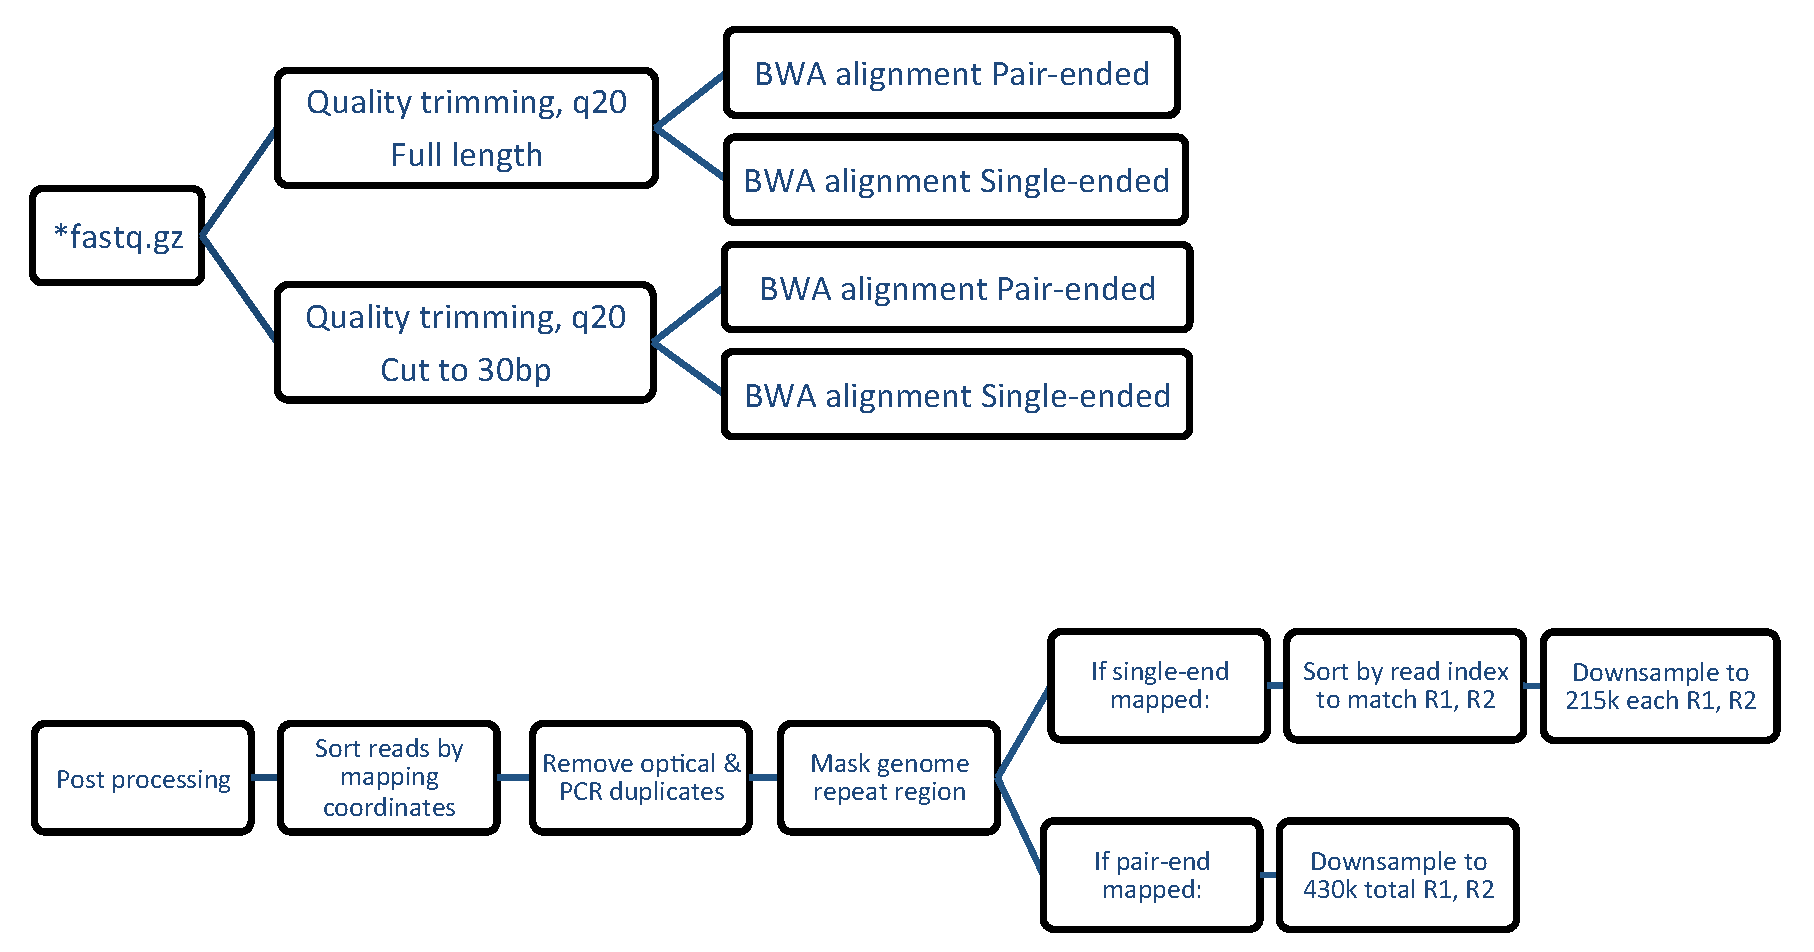
\includegraphics[keepaspectratio,width=\textwidth]{./figures/Chimera_Mapping}
\caption[Bioinformatic workflow for chimera analysis]{Bioinformatic workflow for chimera analysis.}
\label{fig:Chimera_Mapping}
\end{figure}

% Supplementary Text:
% Long-range sequencing technology:
% Recent developments in long-read sequencing, such as PacBio and Nanopore systems, have enabled the detection of chimera in human genome assembly previously made through Illumina short-read data \cite{Pendleton:2015jp}. Long-range sequencing can potentially reduce the amount of chimeric artifacts from PCR-based sequencing library preparation and requires multiple passes of sequencing materials, which is challenging without whole genome amplification.

% One category of TE is called retrotransposon L1, which duplicates through RNA intermediates and reverse transcribes to insert at new genomic locations \cite{Cordaux:2009bb}. L1 has been associated with insertional mutagenesis and is a potential source of genotypic variation among neurons \cite{Evrony:2012dl}. 
\chapter{Conclusion and Future Direction}
In this thesis, a novel single-cell whole genome sequencing technology termed \textit{virtual microfluidics} was developed and applied to enable the study of genomic heterogeneity in complex biological systems. Our technology establishes a new paradigm in single-molecule and single-cell analysis with dramatically different characteristics than established microfluidic approaches. Applications of the technology on purified DNA, cultured bacteria, human gut microbiome samples, and human cell lines demonstrated the robustness of the system. Below, the key findings of this thesis are summarized and possible future research directions are proposed.

\section{Summary of advancements}
\textit{Virtual microfluidics} enables high-throughput nucleic acid digital quantification and whole genome amplification in an easy-to-use, benchtop format that requires no special equipment or environmental control. 

% Besides reducing the production of chimeras in MDA, the unique physical characteristics of the engineered hydrogel environment provide a means for enhancing coverage extent and uniformity from WGA and WTA samples through the self-limiting reactivity within each virtual compartment. In addition, the straightforward addition and removal of reagents to\slash from product clusters \textit{en masse} and excellent optical access ideally suit the \textit{virtual microfluidics} system for rare-cell assays incorporating \textit{in situ} labeling of cells or product clusters. We expect that \textit{Virtual microfluidics} will find application as a low-cost digital assay platform and as a high-throughput platform for single-cell sample preparation. 

\subsection{Enabling the equipment-independent high-throughput DNA target detection}
In chapter 2, we demonstrated \textit{virtual microfluidics} as a robust nucleic acid quantification platform. The dynamic range of the measurement from a tradition method (such as dPCR in droplets or microfluidics devices) for DNA quantification is restricted by the number of partitions, usually up to $10^5$. Due to the nature of \textit{virtual microfluidics}' diffusion-restricted reaction and the continuous virtual chambers, up to 20,000,000 analytes per $\mu$L could be accommodated in our system. Specifically, we tested the performance of in-gel digital PCR and digital MDA as an analytical method for molecular detection and counting. We demonstrated high-throughput digital assays and preparative whole-genome amplification without microfabricated consumables or expensive instrumentation. As few as one DNA target can be detected microscopically with a high signal-to-noise ratio by DNA amplification. The in-gel amplification environment also seals potential infectious targets to minimize the handling of biohazardous materials for infectious disease diagnosis. We expect that \textit{virtual microfluidics} will find application as a low-cost digital assay for detecting DNA biomarkers in the clinic. 

\subsection{Improving the whole genome sequencing data quality and success rate for characterizing uncultured microorganisms}
In chapter 3, we characterized whole genome amplification and recovery of single bacterial genomes for lab-cultured control cells and the human gut microbiome using next-generation sequencing (NGS). Compared to traditional methods of whole genome sequencing on single microbes (in tube and microfluidic device), we improved the uniformity of the whole genome amplification by 25\% $\sim$ 33\% and reduced the rate of the chimeric artifact by a factor of six. The success rate of \textit{virtual microfluidics} single-cell sequencing is about 28\%, which is limited by the Poisson distribution. In contrast, typical success rates (the percentage of amplified genomes that pass purity and genome-size threshold) of single-cell sequencing services provided by large-scale genomic centers based on the first-hand experience from our collaborators is about 10\%. Such genomic centers routinely conduct single-cell sequencing in the clean room and utilize FACS for cell isolation, while our approach has a minimal engineering requirement. We demonstrated single-cell sequencing on human gut microbiome samples and obtained 117 pure single draft genomes. Working with collaborators, we were able to utilize the draft genomes to identify more than 10,000 horizontally transferred genes with unique population-specific and individual-specific features \cite{Brito:2016cd}. We expect that \textit{virtual microfluidics} will find application as a high-throughput platform for single-cell sample preparation to study a diverse collection of uncharacterized microbes and environmental microbiome samples. 

\subsection{Reducing structural variation artifacts for studying human cells using single-cell sequencing}
In chapter 4, we demonstrated \textit{virtual microfluidics} for high-quality single-cell genome sequencing on human cell lines with a 3 $\sim$ 6 fold chimera artifact reduction compared to several single-cell technologies. The chimera reduction feature of the \textit{virtual microfluidics} reduces the false-positive rate of genome structural variation detection in studying tumor clonal heterogeneity. Bioinformatically, we characterized chimeric DNA rearrangements in several recently developed single-cell technologies. The unique chimera signatures across different platforms drew attention to the importance of characterizing chimera artifacts in newly developed single-cell technologies. The hydrogel environment also eliminates the need of creating ultra-small discrete chambers for sub-microliter MDA reactions for comparable high-quality data. Furthermore, all of the preparative steps of single-cell whole genome sequencing are accessible with basic lab equipment. We expect \textit{virtual microfluidics} to be implemented widely by researchers who are interested in studying tumor heterogeneity with single-cell resolution.  
% The digital MDA aspect enables real-time monitoring of the whole genome amplification reaction and could be utilized to determine the fragmentation level of the genome and the extent of amplification.

To summarize, this thesis work centers on the development and demonstration of \textit{virtual microfluidics}, a novel technique for high-quality low-input genomic research. This technique makes single-cell genomics more accessible to a wide range of scientific and biomedical researchers. 

\section{Future direction}
% \subsection{Future applications}
% \subsubsection{}
% \subsubsection{}
% For environmental microbiologists who samples uncharacterized bacteria in the backcountry and on the research vessel
% We expect \textit{virtual microfluidics} find applications as a low-cost, highly accessible digital assay platform that provides superior sensitivity and dynamic range.
% For applications that are sensitive to DNA contaminants, our benchtop technology performance can be further improved by using extra measures against contamination, such as the use of a laminar flow cabinet, separate pre\slash post-amplification laboratories and equipment
\subsection{Future technical improvements of \textit{virtual microfluidics}}
Additional technical improvements are needed in order to realize the full potential of \textit{virtual microfluidics}. To begin, the throughput of \textit{virtual microfluidics} can be improved further. Currently, the primary throughput limitation in the initial demonstration on microbial samples is the volume sub-sampled (60 nL) when product clusters are retrieved, which limits the number of sub-samples that can be retrieved from a single hydrogel. A number of approaches are worth exploring: using a thinner gel with more surface area and\slash or reducing the punch size from the 500 $\mu$ m and 1 mm diameters we employed here could improve throughput. A second possibility could be to use imaging data to guide product retrieval and increase the fraction of retrieved samples containing a single-cell WGA reaction product. The thin hydrogel format affords excellent physical access for imaging, equipment, and reagents, which enables an assortment of sub-sampling approaches including punch\slash pickers, localized hydrogel dissolution, and localized affinity tagging or barcoding. Finally, barcoding approaches could conceivably enable retrieval of all amplified products \textit{en masse} while allowing \textit{in silico} demultiplexing to sort sequence reads according to the cell of origin \cite{Crosetto:2015vd}.

\subsubsection{Suitability of in-gel amplification format for product cluster labeling}
\textit{Virtual microfluidics}'s excellent optical accessibility allows potential fluorescent labeling of rare sequences, which is essential to identify rare targets in microbial dark matter discovery and liquid biopsy applications. For these applications, the demand for single-cell assay throughput is not driven by the need to amass a large number of single-cell datasets, but rather to access cells that are rare in the population. The hydrogel format is ideally suited for this case as the WGA reaction endpoint is an opportune moment to genotype product clusters using hybridization probes in order to identify cells of interest for retrieval and sequencing analysis \cite{Niki:1997vq,Yamada:2011kf}. In the post-reaction hydrogel, genomic sequences have been amplified and are not protected by a cell envelope. In addition, the thin gel slab format facilitates the application of reagents for rapid template denaturation, labeling, and de-staining. Once labeled, the desired targets can be selectively retrieved for further analysis by image-guided selection. Sequence-specific labeling might also reduce the number of false-positive background spots that challenged the intercalating dye-based approach we used in this study and \slash or to lend molecular specificity to quantification assays. In fact, sequential FISH could be used to probe for large sets of functional genes within the gel itself, enabling the application of complex selection criteria \cite{Lubeck:2014jx}. 

\subsubsection{Potential for amplification bias reduction}
Up to 10 pg of DNA is produced by MDA from each template in the hydrogel format using our protocol. Although we re-amplified punch samples in the microbial study to microgram quantities, 10 pg is, in principle, enough product (of an order 1000 bacterial genome equivalents) to support deep sequencing directly. Given that we obtain good coverage distribution with our high-yield re-amplification protocol for bacteria, it may be possible for coverage distribution improvement by direct library construction from the 10 pg hydrogel product. Recent advances in ultra-efficient library construction have demonstrated library construction from sub-nanogram input levels \cite{White:2009jz}. 

Although a number of modified protocols have been proposed to improve coverage distribution in MDA, none has yet been widely adopted, with major single-cell genomics centers continuing to use $\Phi$29 DNA polymerase reaction conditions very similar to those originally developed 30 years ago \cite{Blanco:1985ul,Allen:2011jn}. In contrast, limiting fold-amplification reduces coverage bias, since the ratio of maximum possible fold amplification to minimum possible fold amplification is necessarily reduced when the average degree of amplification is reduced. When combined with the cost savings of micro-scaled reactions and increasingly efficient sequence library construction procedures, such an approach shows the future trend of single-cell WGA \cite{deBourcy:2014ji}. 

Today, investigators limit amplification-fold by reducing reaction volumes \cite{Marcy:2007ip,Landry:2013dh} or by limiting reaction time \cite{Spits:2006em}. Although it is currently unknown which approach is more fruitful in bias reduction, both approaches have drawbacks. The hydrogel reaction format offers unique advantages in limited-extent WGA, as the product clusters from each template molecule only reach a few microns in size, even under dilute template conditions. This suggests that one can achieve uniform (limited) reaction extent across single-cell WGA reactions, even when the reactions occur asynchronously. The hydrogel format also enables maintenance of optimal amplification conditions for each template throughout the reaction time course if desired by reagent supplementation, possibly reducing sequence content and template fragment length biases. In order to further measure the amplification bias in the hydrogel, a random barcode library can be introduced into the hydrogel for amplification and sequencing analysis. 

\subsection{The future of single-cell whole genome sequencing}
The single-cell sequencing process from having cells in suspension to obtaining sequencing data is highly fragmented in terms of technology implementation. On the other hand, due to the diverse applications of single-molecule and single-cell analysis, it is difficult to find a one-tool-fits-all solution. The key is to have a platform technology that allows modular changes of different processes involved, in order to strike a balance among the requirements of throughput, hands-on time, cost, and quality for various applications. This reality also explains the slow uptake of single-cell technology in various research and clinical settings. To address these issues, \textit{virtual microfluidics} represents a platform technology that can be implemented with a diverse collection of methods in cell lysis, whole genome amplification, and barcoding strategies. With further technical optimizations, this technique could play a central role in integrating the single-cell sequencing field.

% Beyond the traditional method of whole genome amplification on isolated single cells, I envision that it will be ideal to barcode a large number of single cells with minimal amplification and obtain accurate long-read sequencing results. Such a technology combination will revolutionize the landscape of single-cell sequencing. Because it minimizes the biases and artifacts from extensive amplification that often distort the output data from the original genomic sequences. Long-read sequencing (currently 10 kbp - 400 kbp) has the advantage of providing the genuine read of a long genome sequence that could be highly repeated and of high GC\%, which are challenging for the current short-read technologies (50 bp - 500 bp). At the same time, it also requires the development of more accurate sequencing technologies. Currently PacBio (long-read) has an error rate of $\sim 10\%$, compared to the 0.1 $\sim$ 1 \% of the short-read Illumina sequencing. A recent development has demonstrated direct library preparation on single cells in nano-droplets for whole genome sequencing \cite{Zahn:2017fb}. Its performance is below that of state of the art single-cell technologies, in terms of genome physical coverage and coverage uniformity. However, the concept of direct library preparation on a large number of samples (hundreds) without the expensive and often biased WGA process is attractive to researchers to obtain the most representative genomic information. 

% Beyond single-cell sequencing, there still exist challenges in implementing genomic testing in the clinic as the standard of care. First of all, the reimbursement and clinical adoption reply on the innovation of the sequencing cost reduction. Secondly, it is difficult for patients, doctors and researchers who lack the genomic related training to interpret the data. This is especially critical when doctors and patients have to make decisions with the consideration of the inherent false-positive and false-negative rate of the genomic data. 
% Furthermore, a large percentage (40$\%$ - 60$\%$) of patients often don't have actionable mutations according to recent cancer sequencing projects (GenomeWeb Mar 01, 2017). The uptake of standard genomic technologies will likely develop hand-in-hand with genomic-guided and targeted drug discovery. With the growing of related products such as 23andMe, and genomic service companies such as Foundation Medicine, Grail, and Color Genomics, the share of genomic data to promote research and diagnosis will spread rapidly. In my opinion, the future of single-cell sequencing field relies on the uptake of standard genomic technologies, in addition to more single-cell analysis innovations, in order to realize its full potential.  
% % I feel like it would be nice to fit your work a little more closely with your conclusion somehow.
% % \subsubsection{The origin story of \textit{virtual microfluidics}}
% % In 2012, I started testing the DNA amplification in the hydrogel with a project code name \say{matrix digital}. The goal was to achieve a sub-cellular resolution for \textit{in-situ} RNA molecule counting. However, optimizing the hydrogel for 



\appendix
\chapter{NCBI accession numbers}
\section{Bacterial single cells}
Raw sequencing data on \textit{E. coli} and \textit{S. aureus} are accessible at the NCBI Sequence Read Archive (SRA) under BioProject accession number PRJNA279815 with BioSample accession numbers SAMN03451478-SAMN03451501. FijiCOMP metagenomic reads can be found under BioProject accession number PRJNA217052 with the accession numbers: SRX345831, SRX344363, SRX344765, SRX343094, SRX344442, SRX346405, SRX343839, SRX343780, SRX345901, SRX344600, SRX343866, SRX343411, SRX344189, SRX344380, SRX346966, SRX345329, SRX343800, and SRX344616. FijiCOMP \textit{virtual microfluidics} 117 single cells are accessible with the BioSample accession numbers SAMN04461233-SAMN04461349.

\section{Human single cells}
Raw sequencing data on RPE-1 bulk genomic DNA and single cells using \textit{virtual microfluidics} are accessible under BioProject accession number PRJNA408301 with BioSample accession numbers SAMN07682898 and SAMN07682891. 

\begin{table}
\caption{SRA accession numbers for human single-cell chimera analysis}
\label{tab:SRAaccession}
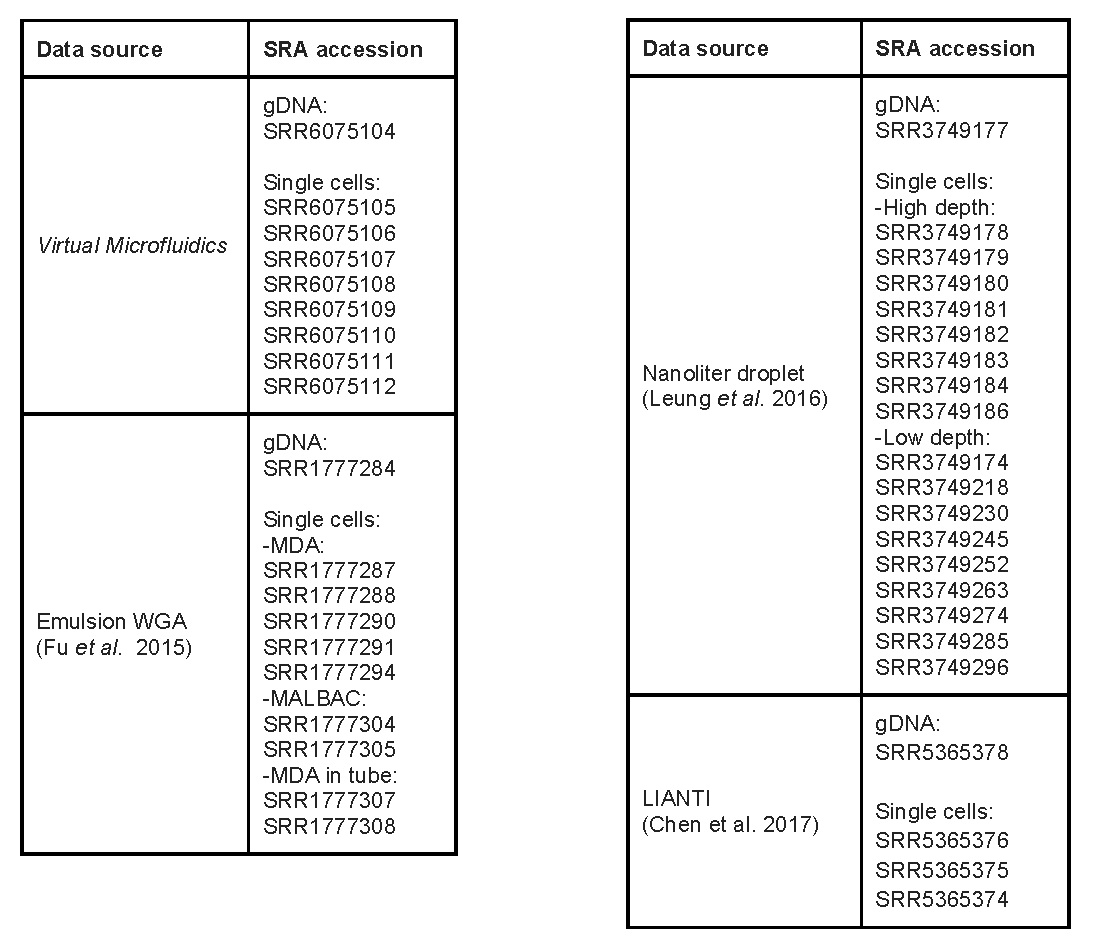
\includegraphics[width=0.8\linewidth]{./figures/SRAaccession}
\end{table}

% \begin{table}
% \centering 
% \caption{QPCR characterization of hydrogel punches}
% \label{tab:QpcrHydrogel}
% \begin{adjustbox}{max width=0.7\textwidth}
% \begin{tabular}{c||c} 

% \hline 
% Total hydrogel punches & 80 \\ 
% \hline
% \textit{E. coli} positive punches & 7  \\
% \hline
% \textit{S. aureus} positive punches & 36 \\
% \hline
% Double positive & 7 \\
% \hline
% Double negative & 30 \\
% \hline
% \end{tabular}
% \end{adjustbox}
% \end{table}

% \begin{table}
% \caption{PCR primer sequences}
% \label{tab:ESprimerList}
% \begin{center}
% \includegraphics[width=0.5\linewidth]{./figures/ESprimerList}
% \end{center}
% \end{table}

% \begin{table}
% \caption{Mapping statistics, \textit{E. coli} and \textit{S. aureus}}
% \label{tab:MapStatES}
% \includegraphics[width=\linewidth]{./figures/MapStatES}
% \end{table}

% \begin{table}
% \caption{Sequence read classification \say{other reads}, \textit{E. coli} and \textit{S. aureus}}
% \label{tab:OtherReadsES}
% \includegraphics[width=\linewidth]{./figures/OtherReadsClassificationES}
% \end{table}

% \begin{table}
% \caption{Downsampling on mapped reads from single-cell MDA samples}
% \label{tab:DownsamplingESD}
% \includegraphics[width=\linewidth]{./figures/DownsamplingESdeBourcy}
% \end{table}

% \begin{table}
% \caption{Metagenomic shotgun profiling weighted with single-cell samples}
% \label{tab:MetagenomicFiji}
% \includegraphics[width=\linewidth]{./figures/MetagenomicShotgunProfilingFiji}
% \end{table}

% \begin{table}
% \caption{Data source for chimera analysis}
% \label{tab:chimeraDataSource}
% \includegraphics[width=\linewidth]{./figures/Chimera_DataSource}
% \end{table}

% \begin{table}
% \caption{Single-cell technology comparisons for chimera analysis}
% \label{tab:chimeraTechTable}
% \includegraphics[width=\linewidth]{./figures/Chimera_TechTable}
% \end{table}

\clearpage
%% This defines the bibliography file (main.bib) and the bibliography style.
%% If you want to create a bibliography file by hand, change the contents of
%% this file to a `thebibliography' environment.  For more information 
%% see section 4.3 of the LaTeX manual.
\begin{singlespace}
\bibliography{Thesis}
\bibliographystyle{unsrt}
\end{singlespace}

\end{document}

